\subsection{First \glsentrytext{slam} path using the Pioneer robot at 26 cm/s}

The figures in this section show the detailed results of the test performed with the Pioneer robot with a 25 mm resolution map in the industrial hall following the first \gls{slam} path and moving at 26 cm/s.


%Animated paths
\begin{figure}[H]
	\centering
	\animategraphics[width=0.65\textwidth,loop,autoplay,controls]{1}{appendices/tests-3dof/pioneer-robot/\currfilebase/images-ground-truth/image}{1}{20}
	\caption{Laser scans projected on top of the map using the ground truth poses}
\end{figure}

\begin{figure}[H]
	\centering
	\animategraphics[width=0.65\textwidth,loop,autoplay,controls]{1}{appendices/tests-3dof/pioneer-robot/\currfilebase/images-drl/image}{1}{20}
	\caption{Laser scans projected on top of the map using the localization system poses}
\end{figure}

\begin{figure}[H]
	\centering
	\animategraphics[width=0.65\textwidth,loop,autoplay,controls]{1}{appendices/tests-3dof/pioneer-robot/\currfilebase/images-amcl/image}{1}{20}
	\caption{Laser scans projected on top of the map using the \glsentrytext{amcl} poses}
\end{figure}


%Laser assembly
\begin{figure}[H]
	\centering
	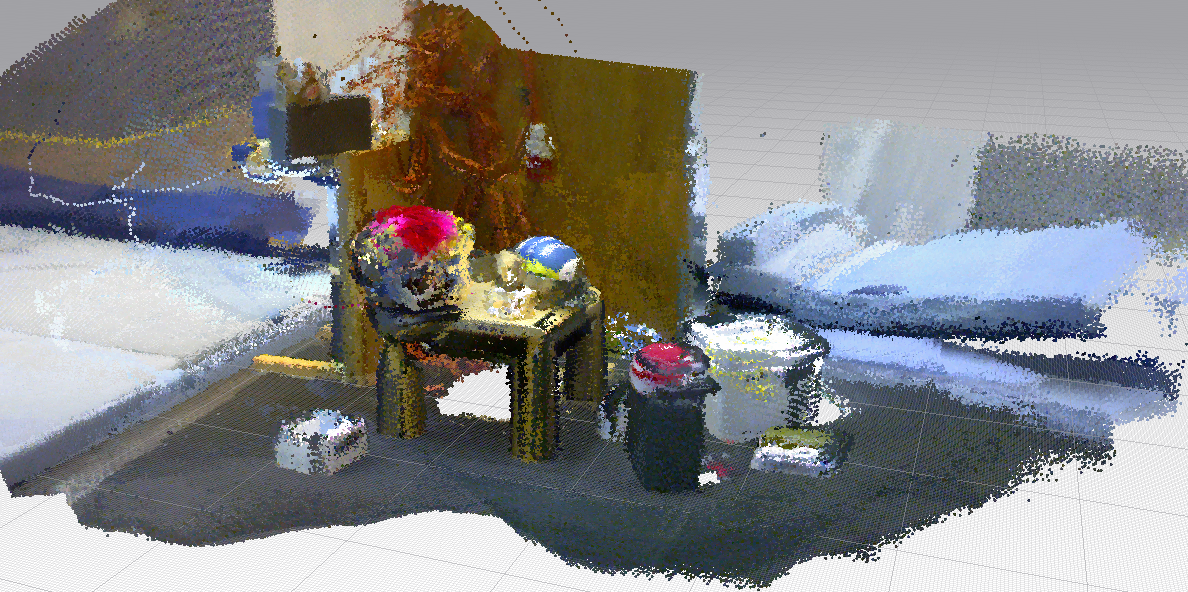
\includegraphics[width=0.91\textwidth]{appendices/tests-3dof/pioneer-robot/\currfilebase/ground-truth-cumulative}
	\caption{Laser scans assembled on top of the map using the ground truth poses}
\end{figure}

\begin{figure}[H]
	\centering
	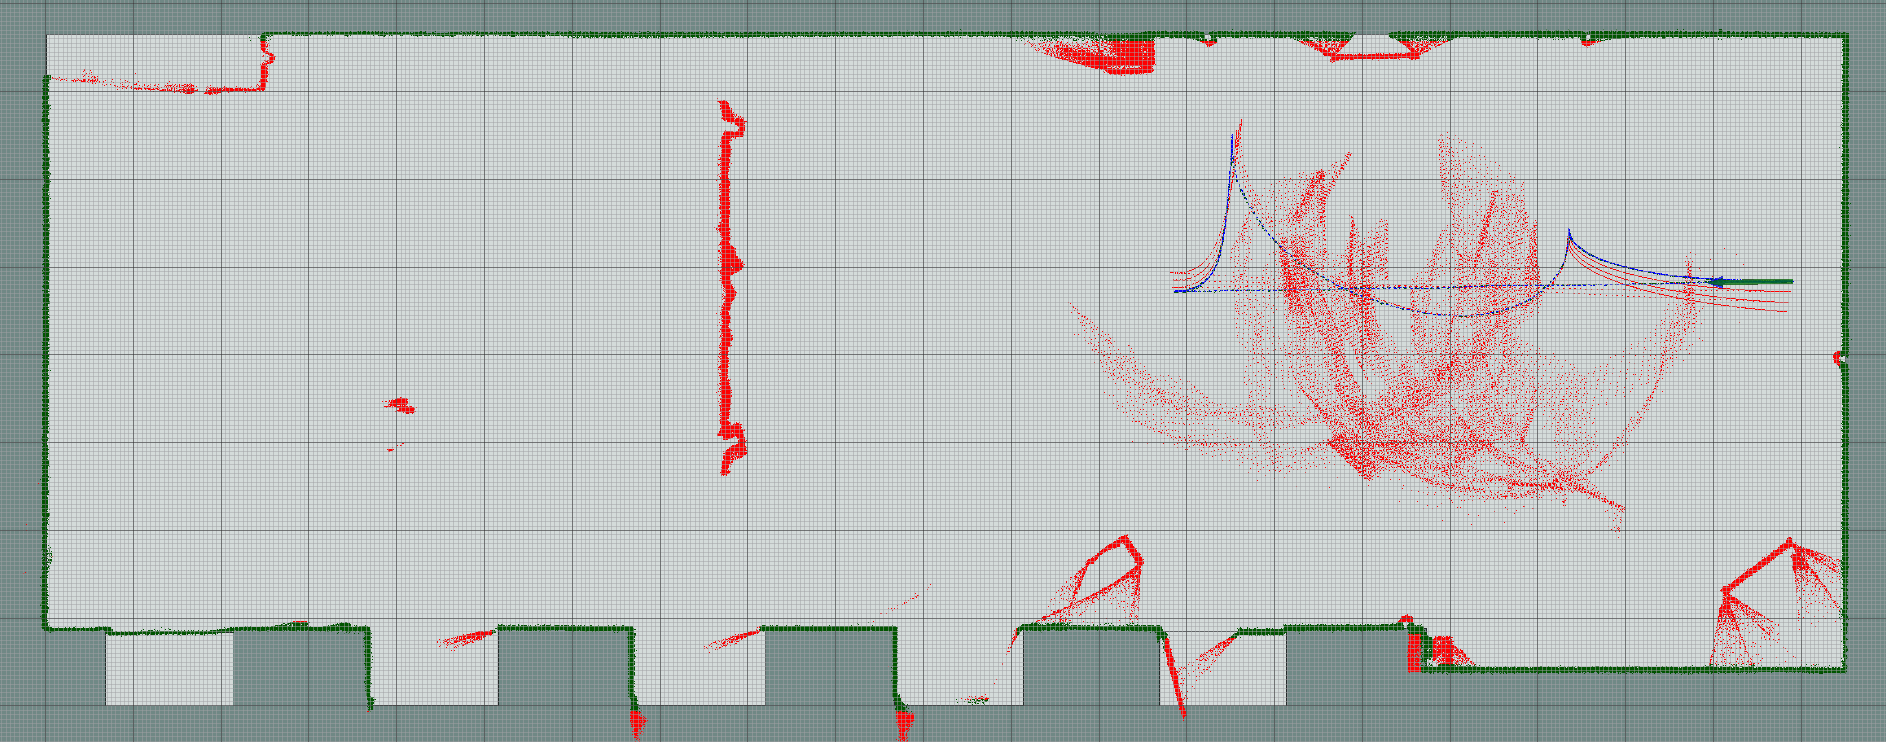
\includegraphics[width=0.91\textwidth]{appendices/tests-3dof/pioneer-robot/\currfilebase/drl-cumulative}
	\caption{Laser scans assembled on top of the map using the localization system poses}
\end{figure}

\begin{figure}[H]
	\centering
	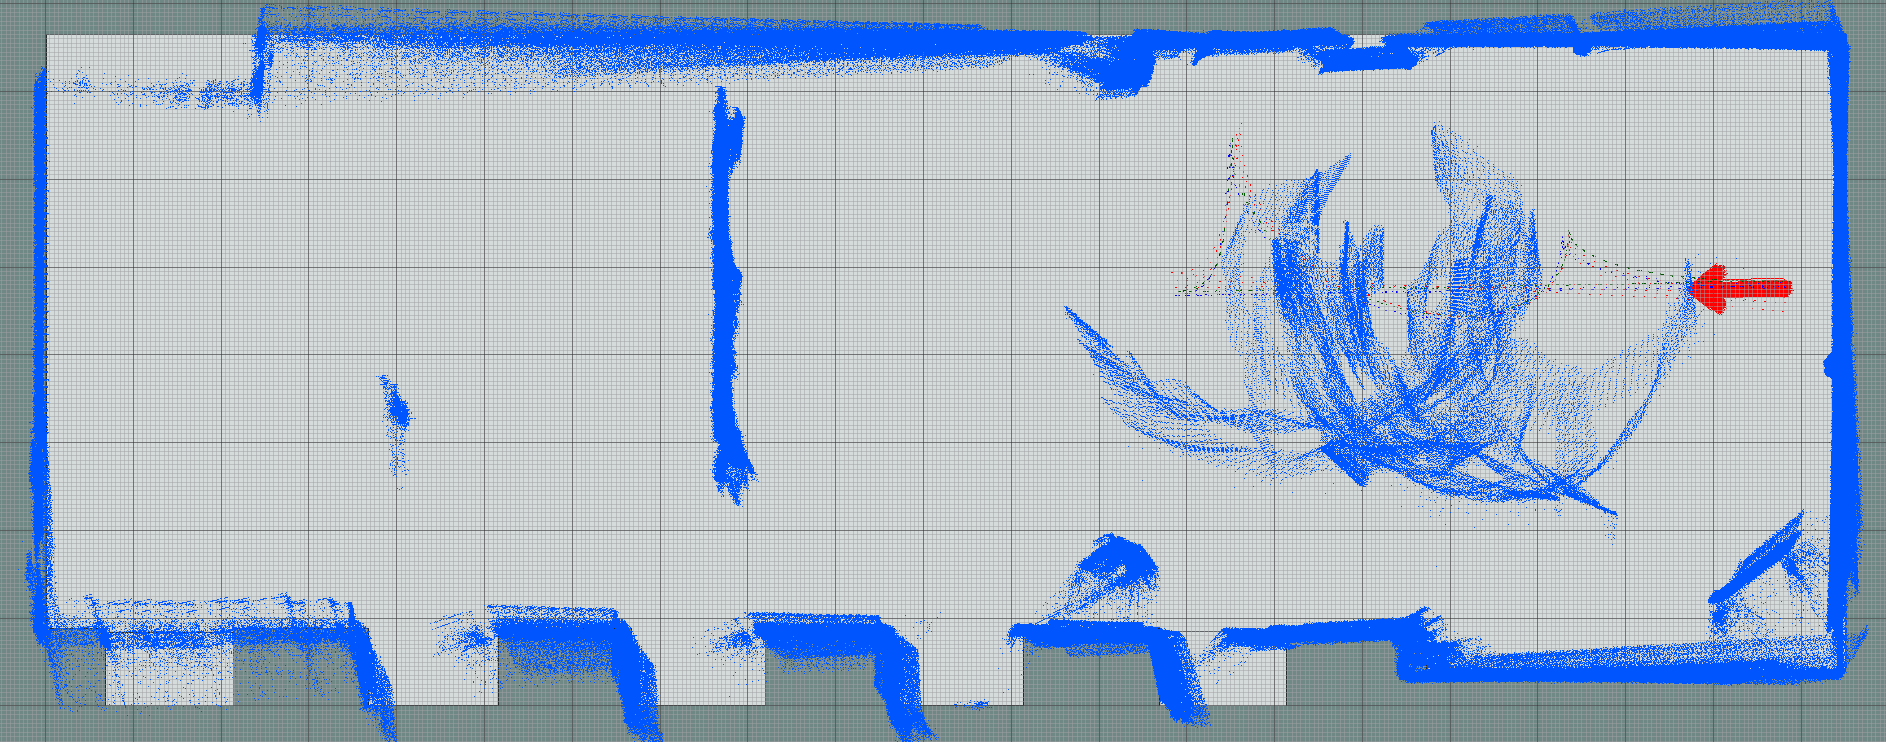
\includegraphics[width=0.91\textwidth]{appendices/tests-3dof/pioneer-robot/\currfilebase/amcl-cumulative}
	\caption{Laser scans assembled on top of the map using the \glsentrytext{amcl} poses}
\end{figure}


%Paths
\begin{figure}[H]
	\centering
	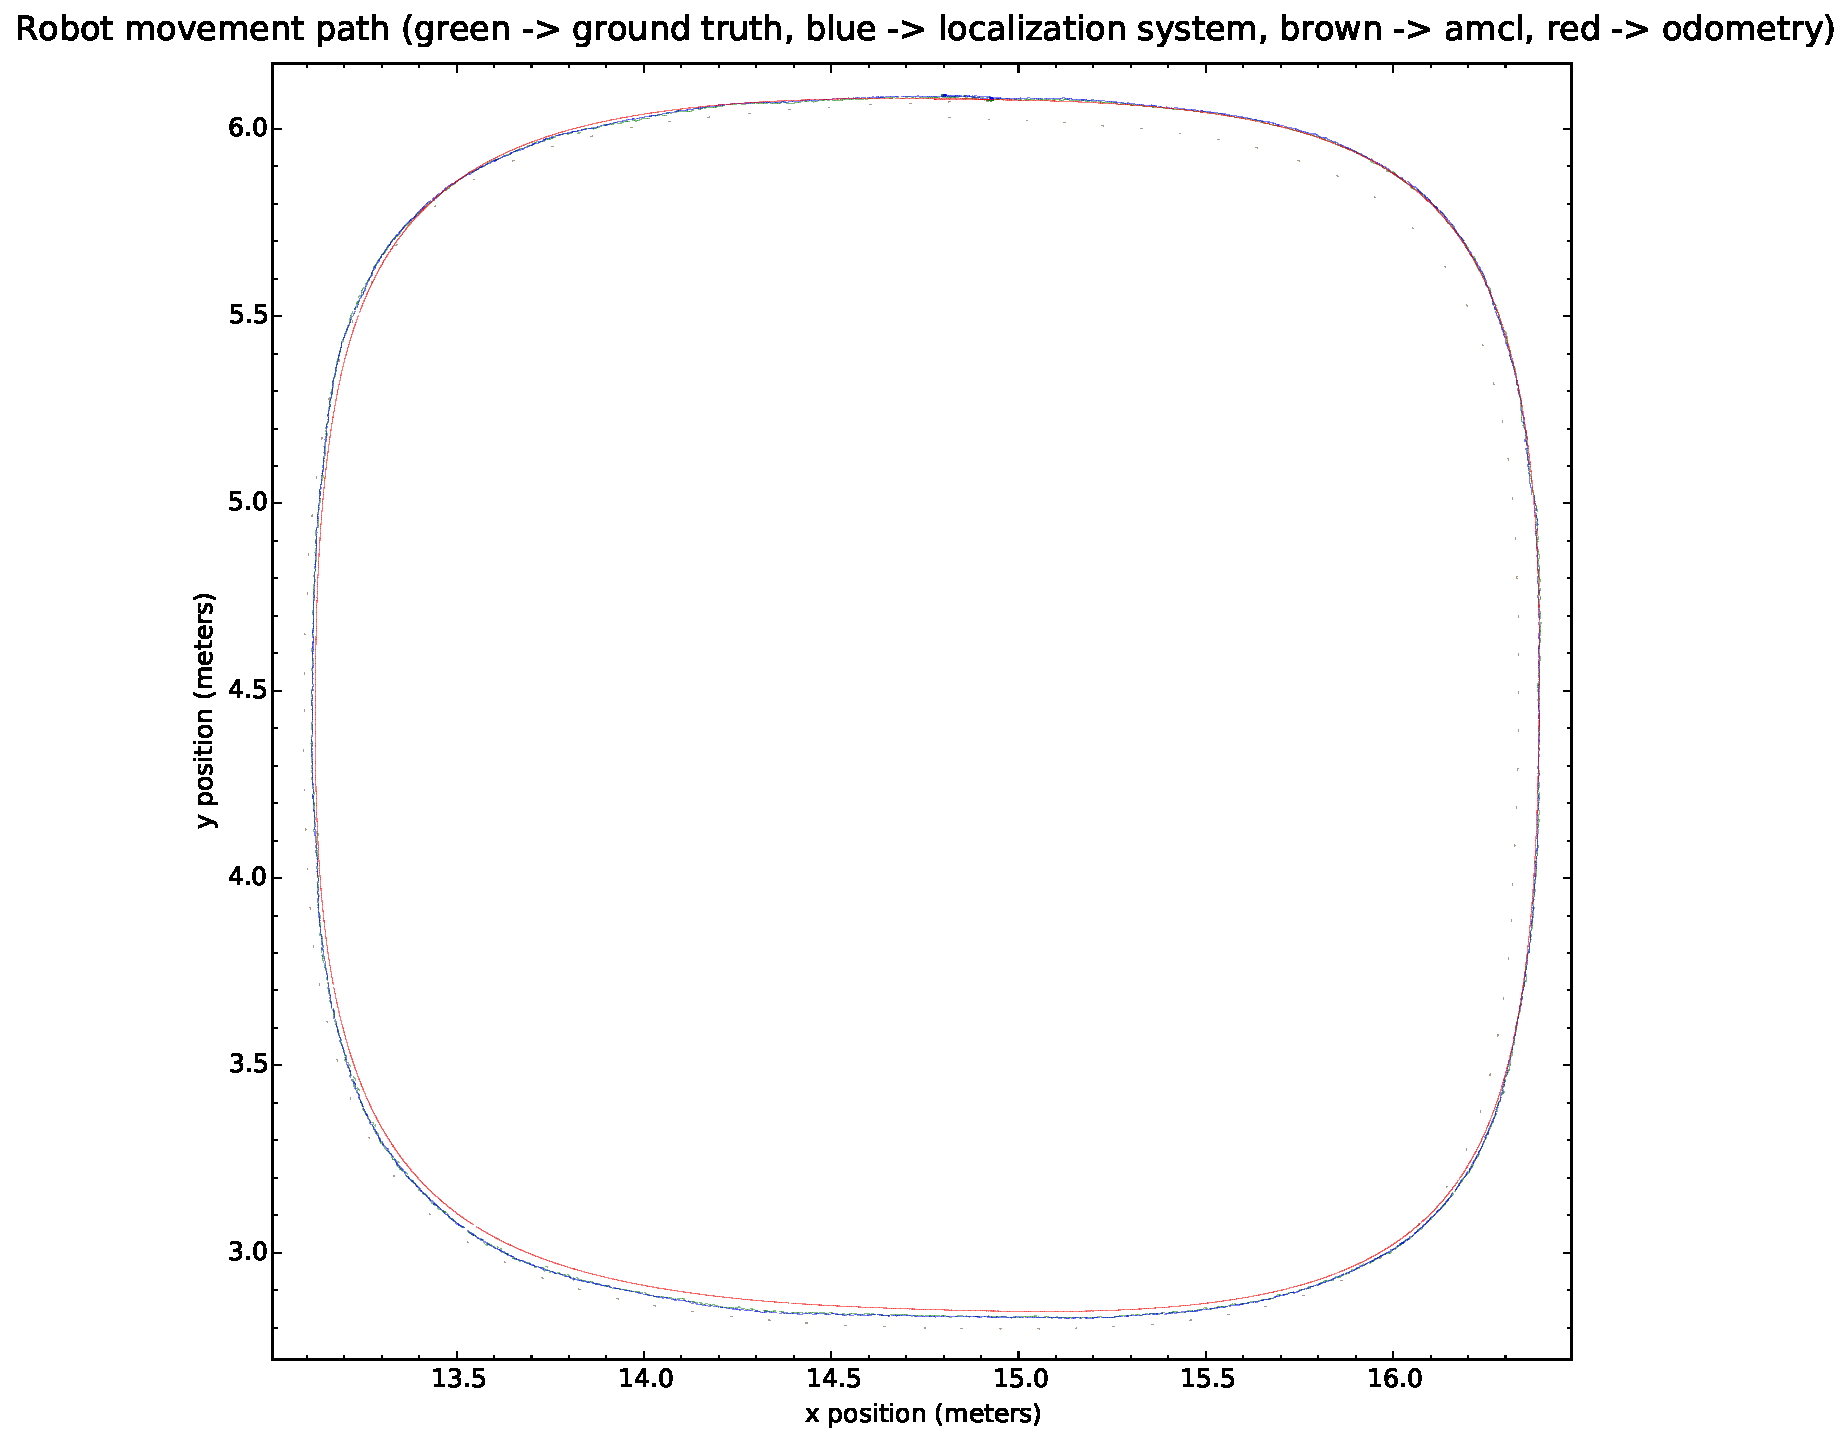
\includegraphics[width=0.8\textwidth]{appendices/tests-3dof/pioneer-robot/\currfilebase/graphs/robot-movement-path-with-odometry-and-amcl}
	\caption{Poses estimated by the ground truth, localization system, \glsentrytext{amcl} and odometry}
\end{figure}

\begin{figure}[H]
	\centering
	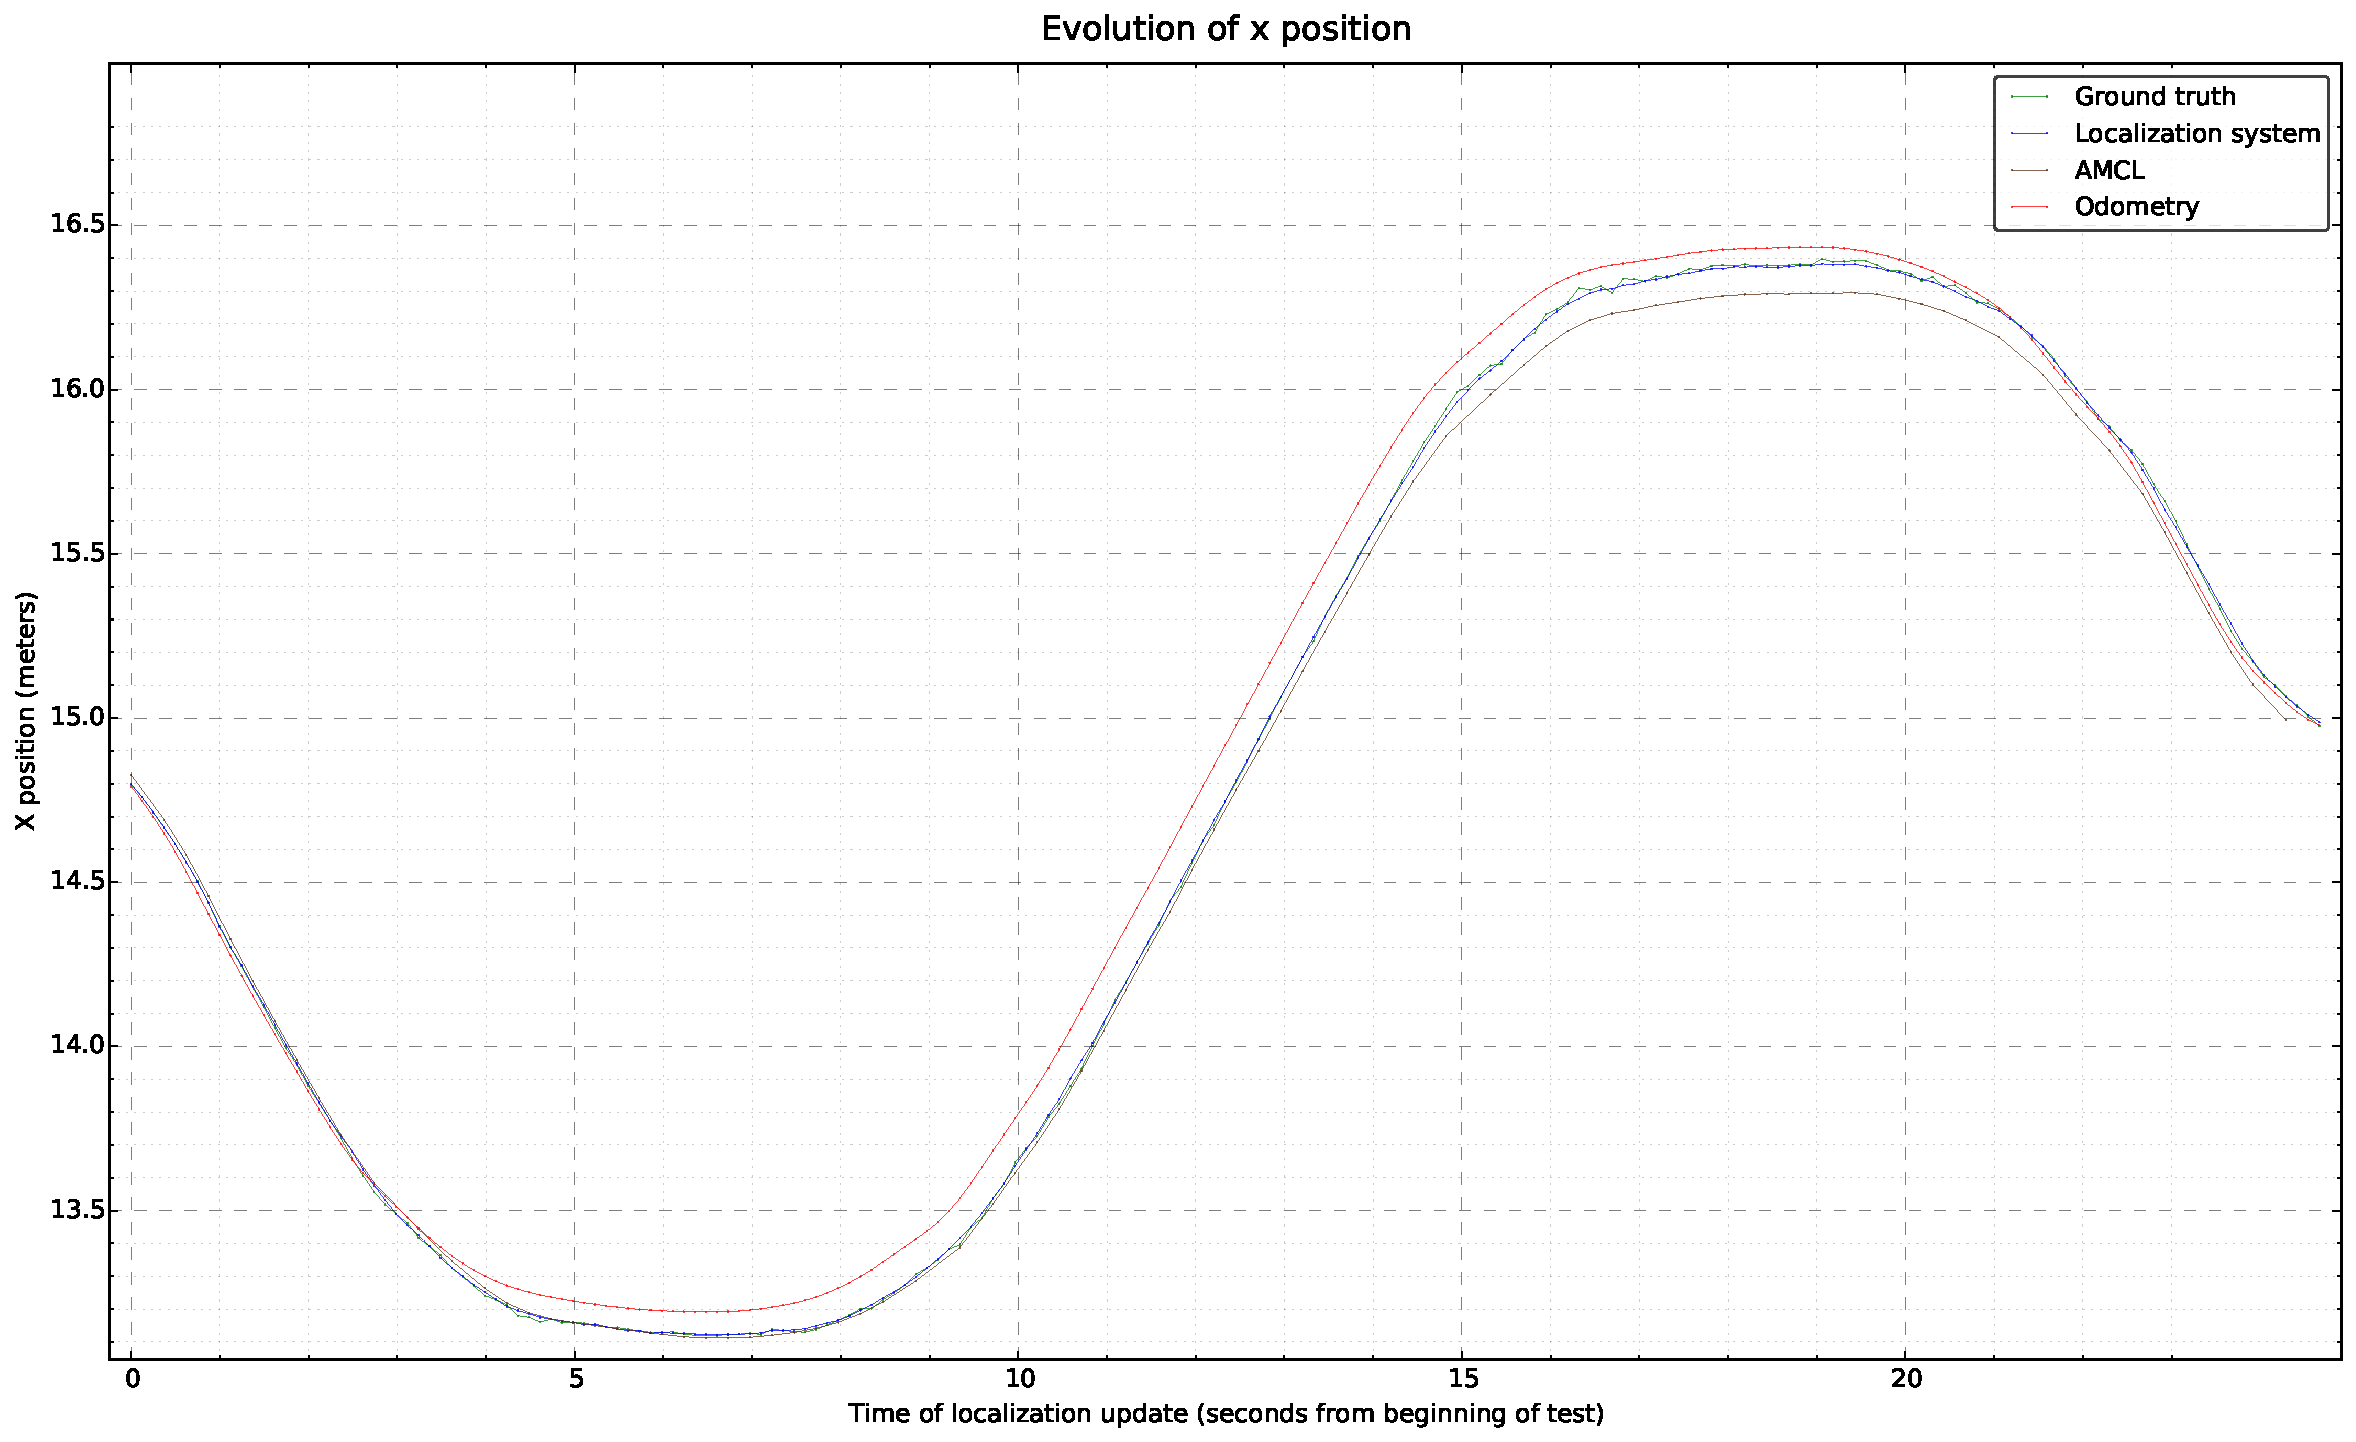
\includegraphics[width=0.53\textwidth]{appendices/tests-3dof/pioneer-robot/\currfilebase/graphs/robot-movement-path-position-evolution-x-with-amcl}
	\caption{Evolution of x position over time}
\end{figure}

\begin{figure}[H]
	\centering
	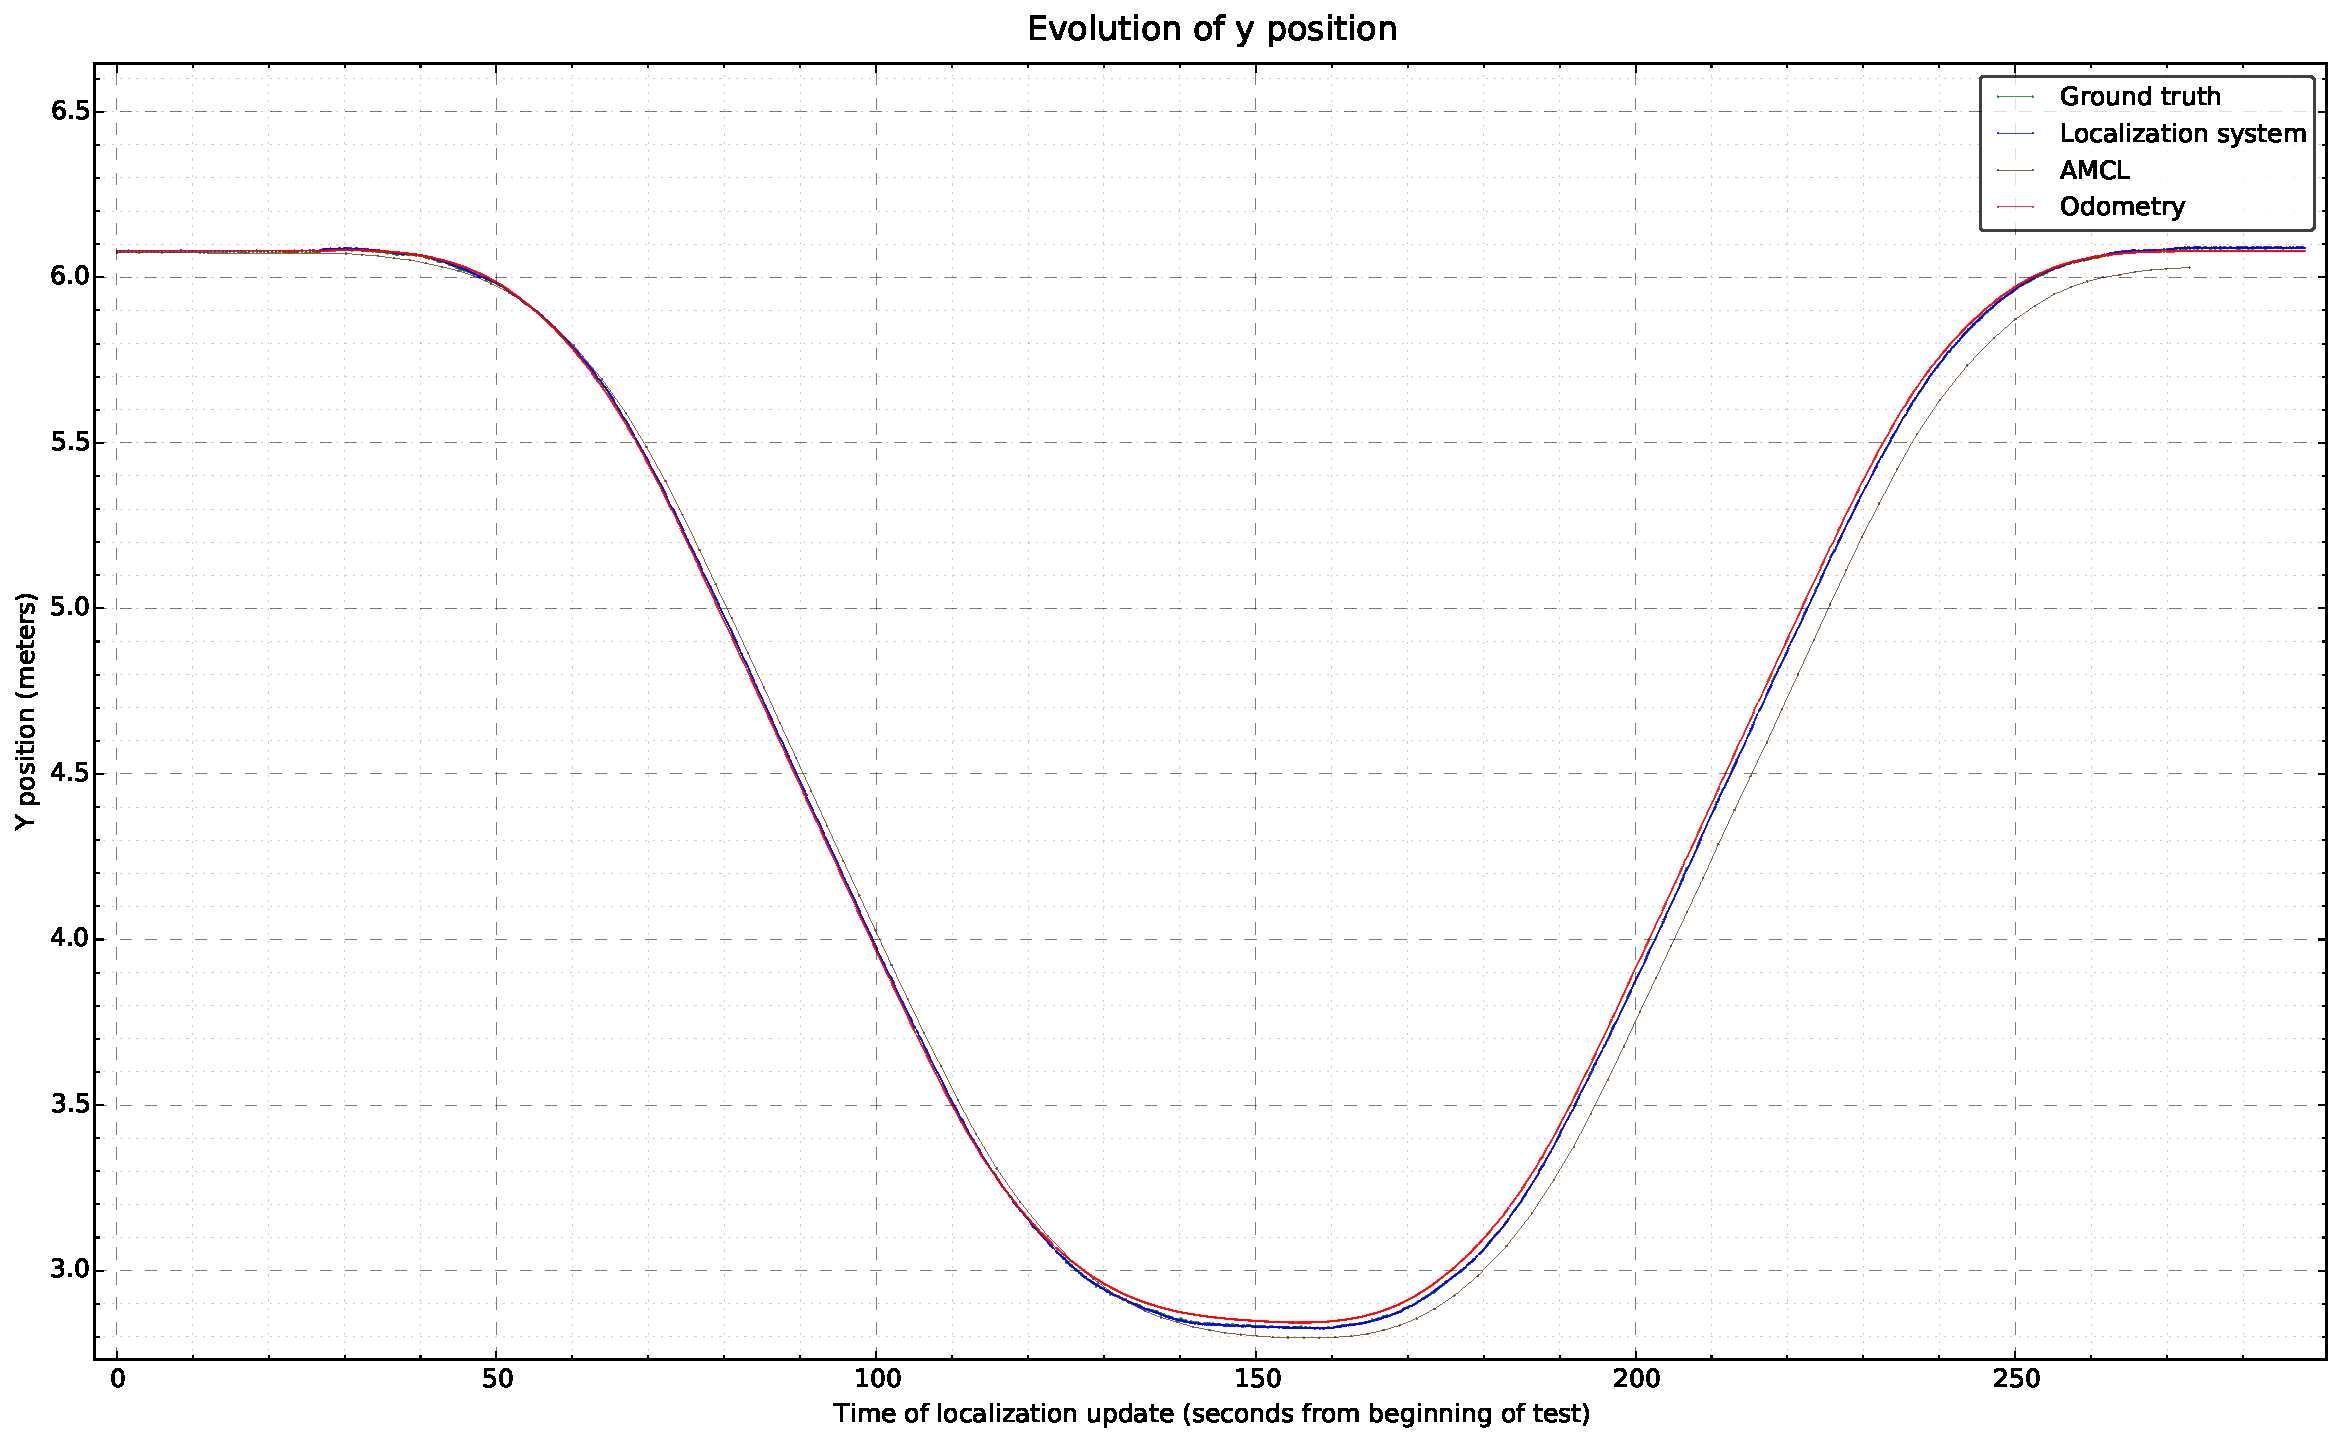
\includegraphics[width=0.53\textwidth]{appendices/tests-3dof/pioneer-robot/\currfilebase/graphs/robot-movement-path-position-evolution-y-with-amcl}
	\caption{Evolution of y position over time}
\end{figure}


%Distance derivatives
\begin{figure}[H]
	\centering
	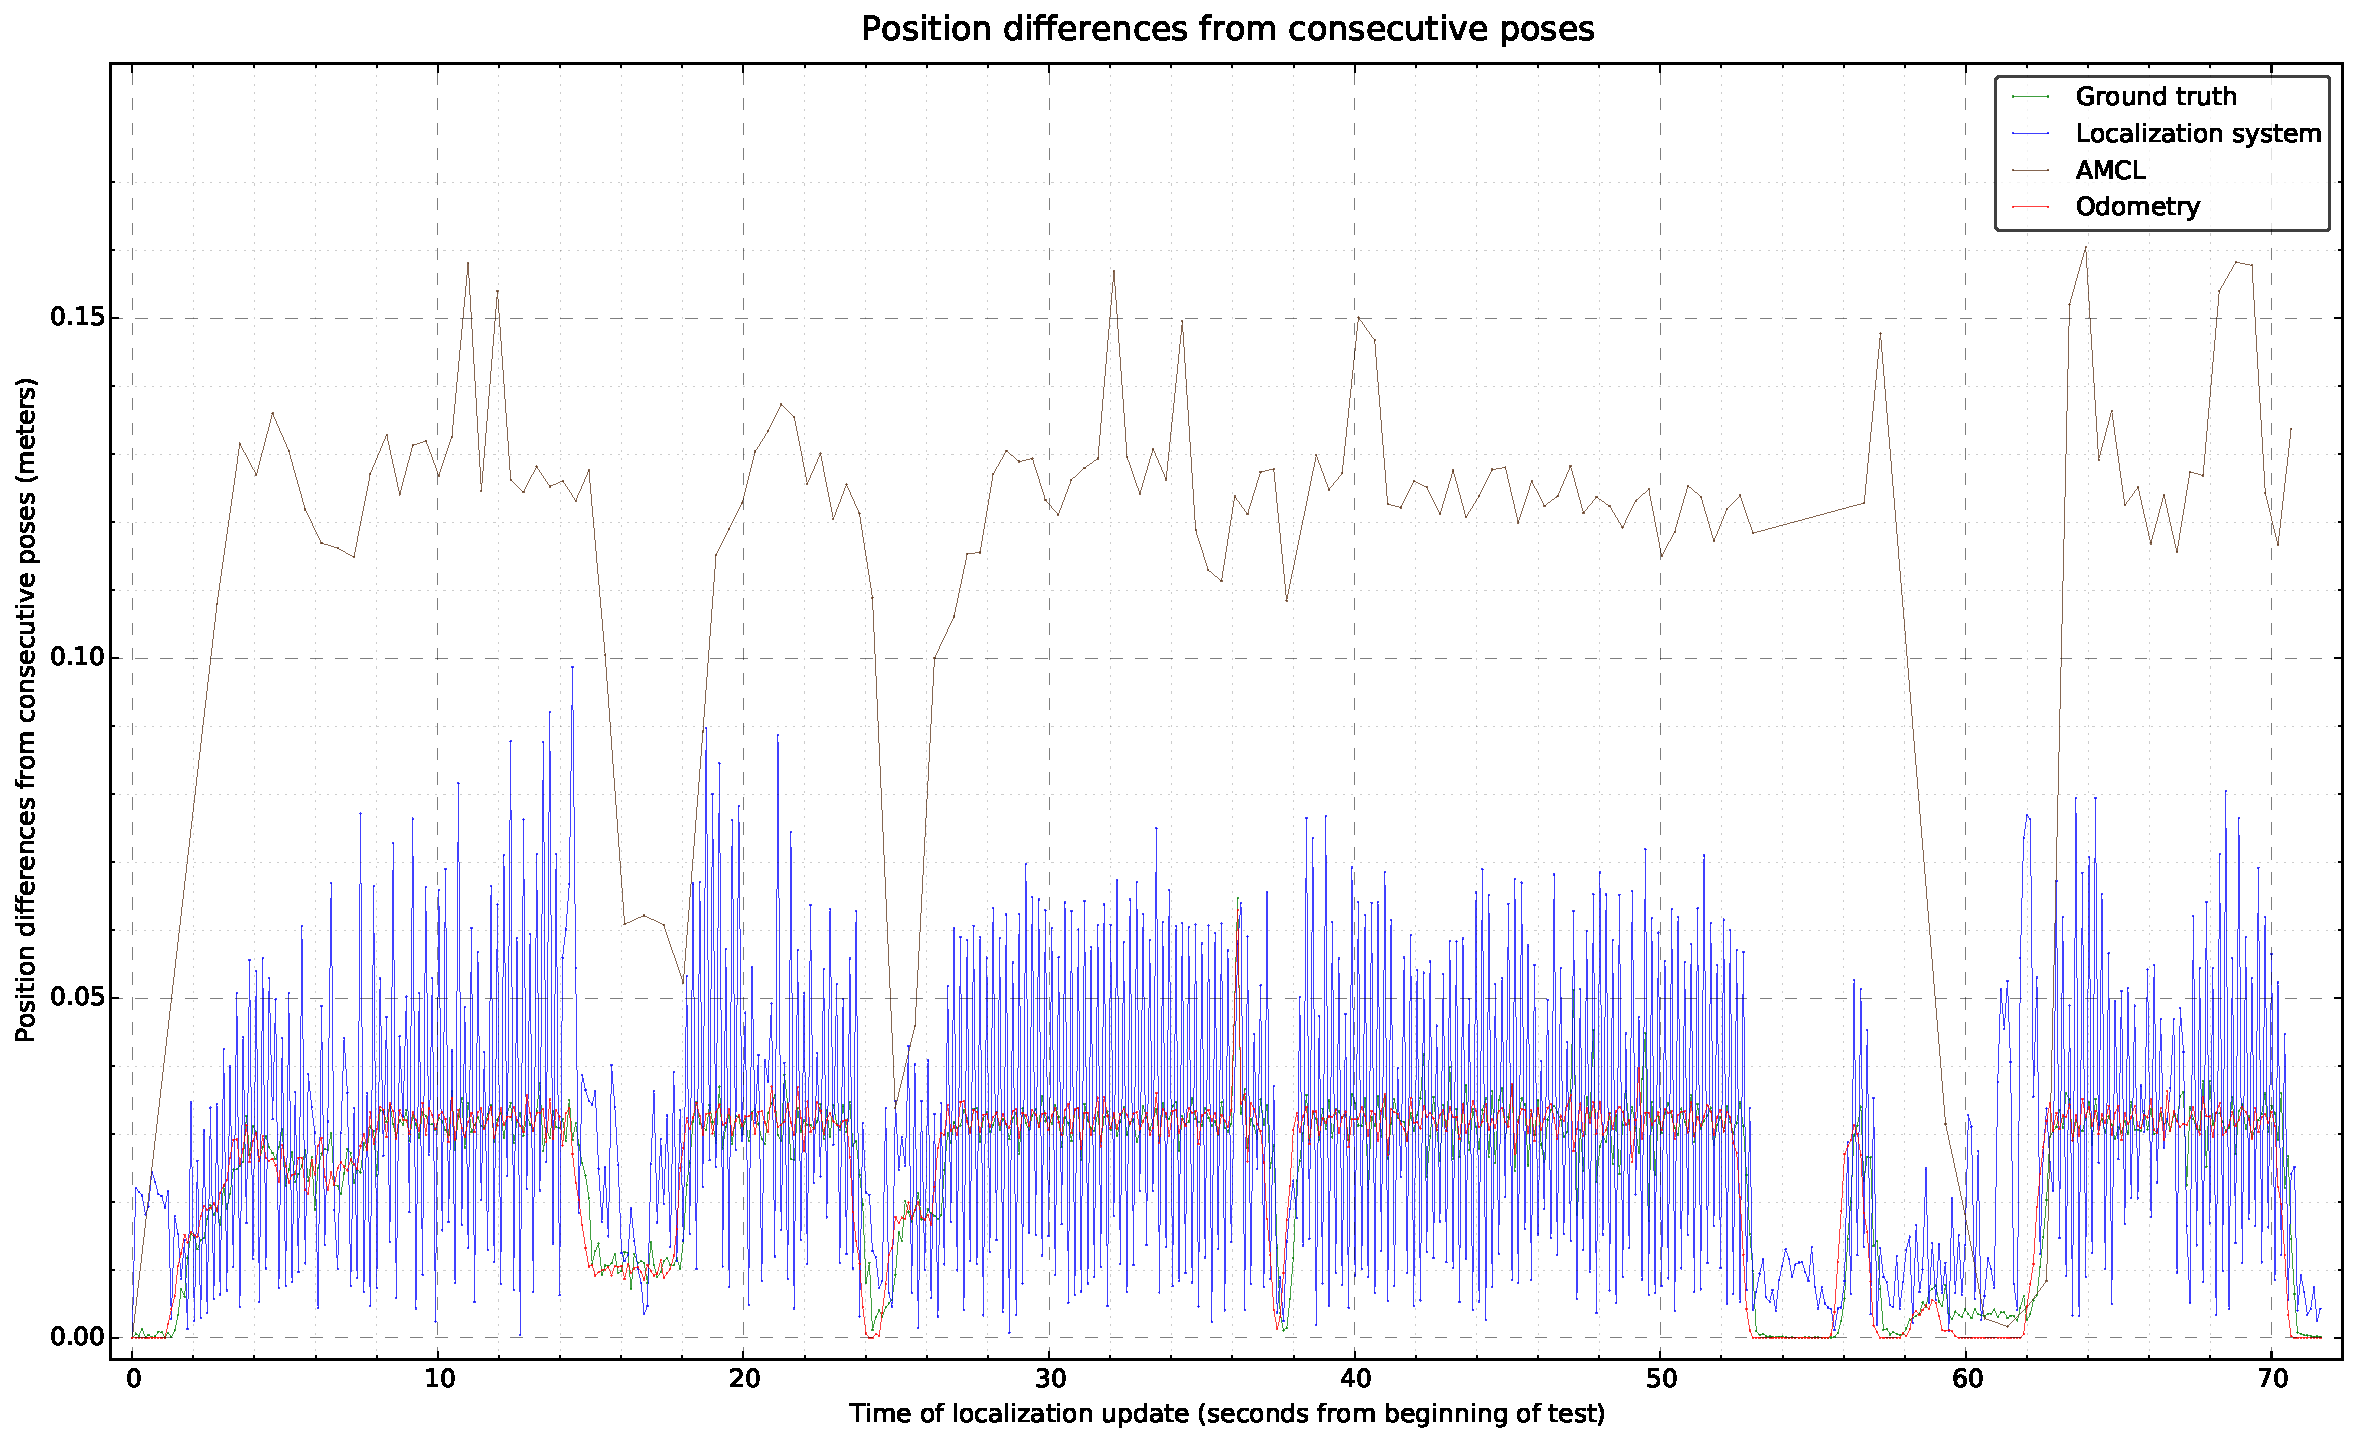
\includegraphics[width=0.7\textwidth]{appendices/tests-3dof/pioneer-robot/\currfilebase/graphs/robot-movement-path-position-differences-with-amcl}
	\caption{Distance traveled between consecutive pose estimations}
\end{figure}

\begin{figure}[H]
	\centering
	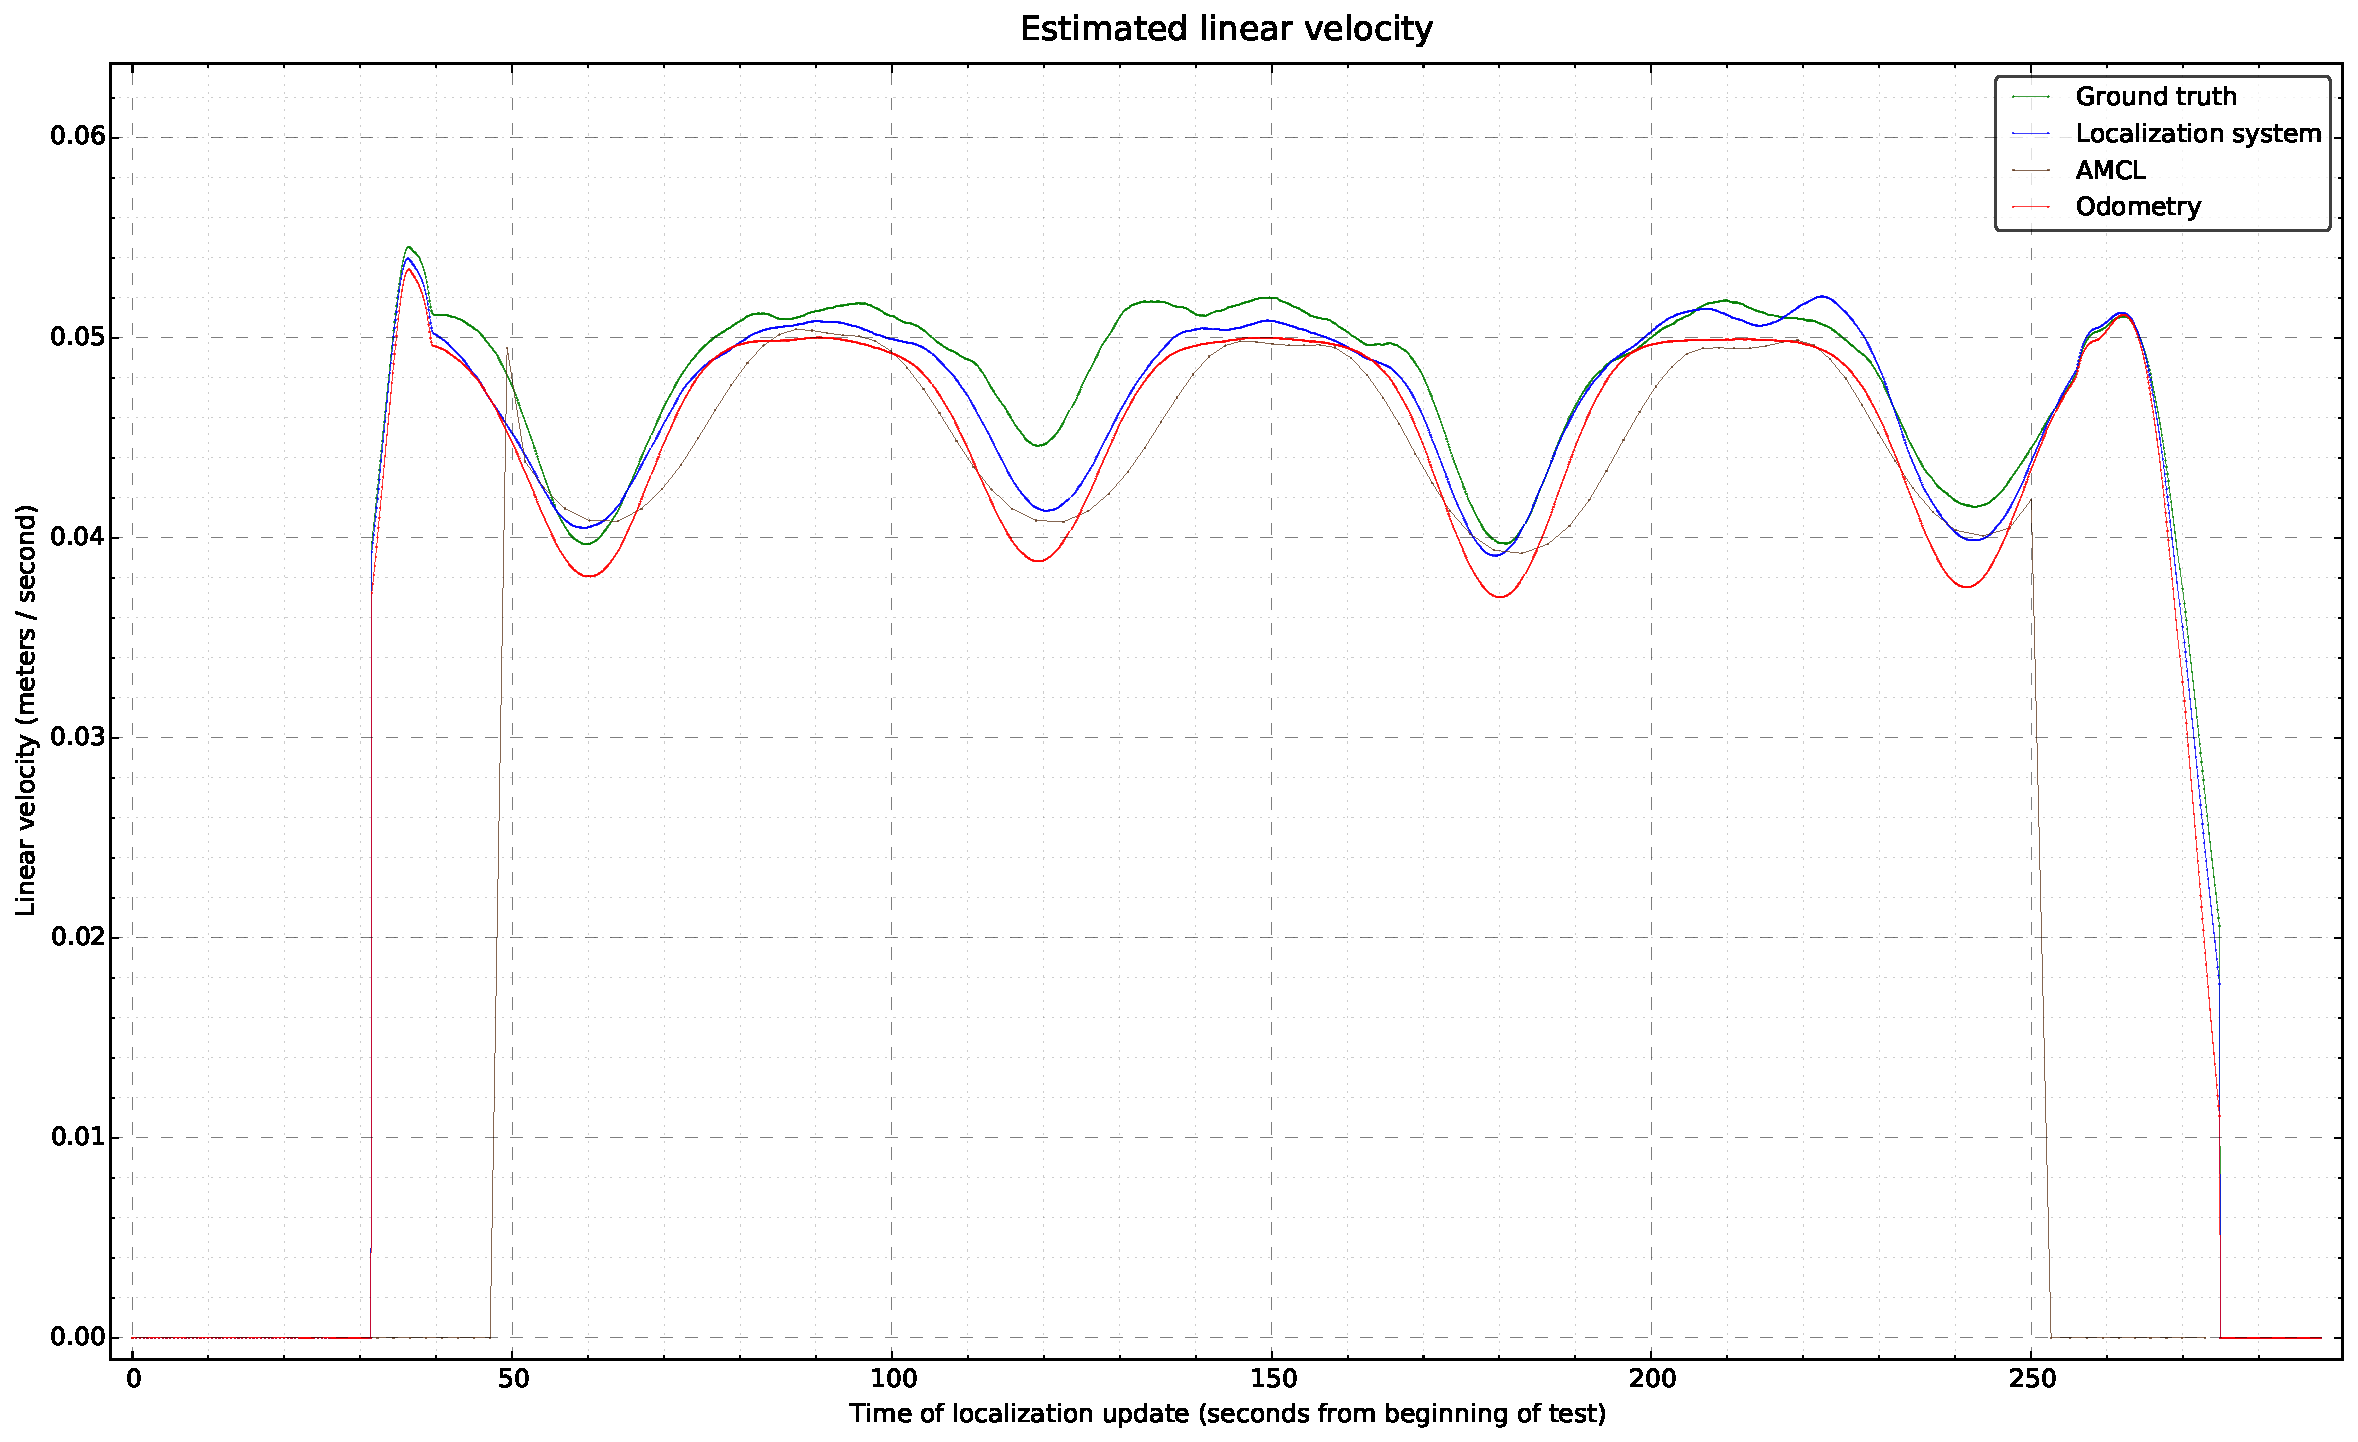
\includegraphics[width=0.7\textwidth]{appendices/tests-3dof/pioneer-robot/\currfilebase/graphs/robot-movement-path-linear-velocity-with-amcl}
	\caption{Estimated linear velocity}
\end{figure}

\begin{figure}[H]
	\centering
	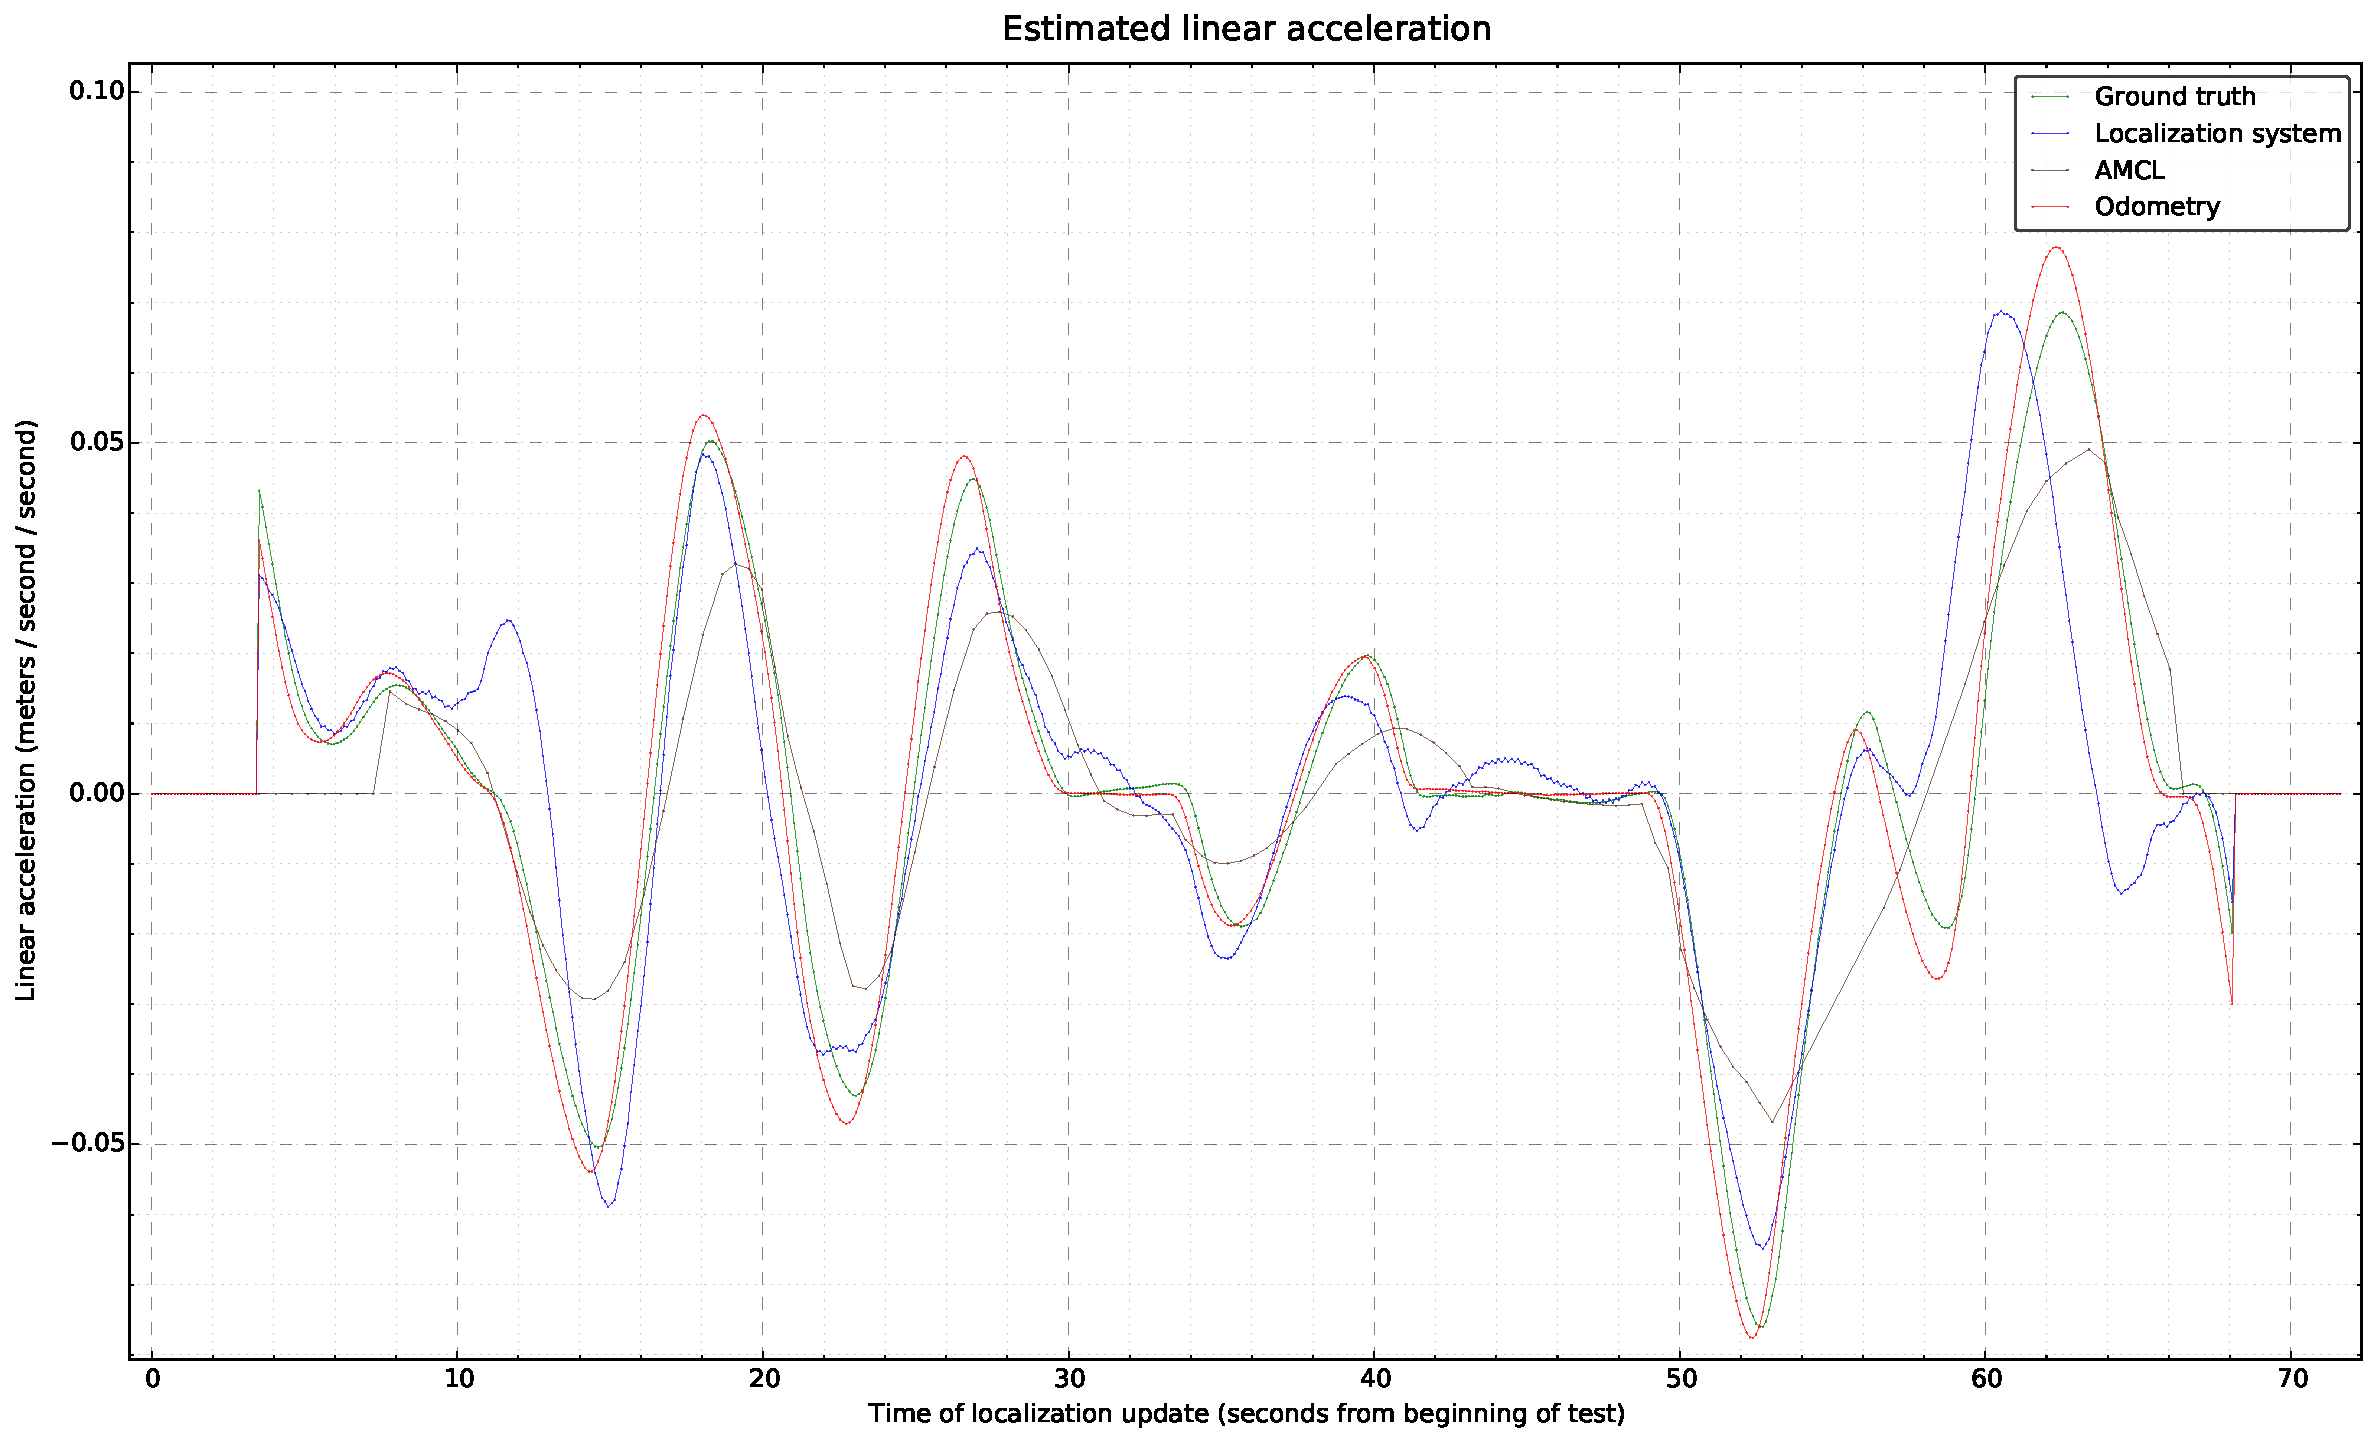
\includegraphics[width=0.7\textwidth]{appendices/tests-3dof/pioneer-robot/\currfilebase/graphs/robot-movement-path-linear-acceleration-with-amcl}
	\caption{Estimated linear acceleration}
\end{figure}


%Angular derivatives
\begin{figure}[H]
	\centering
	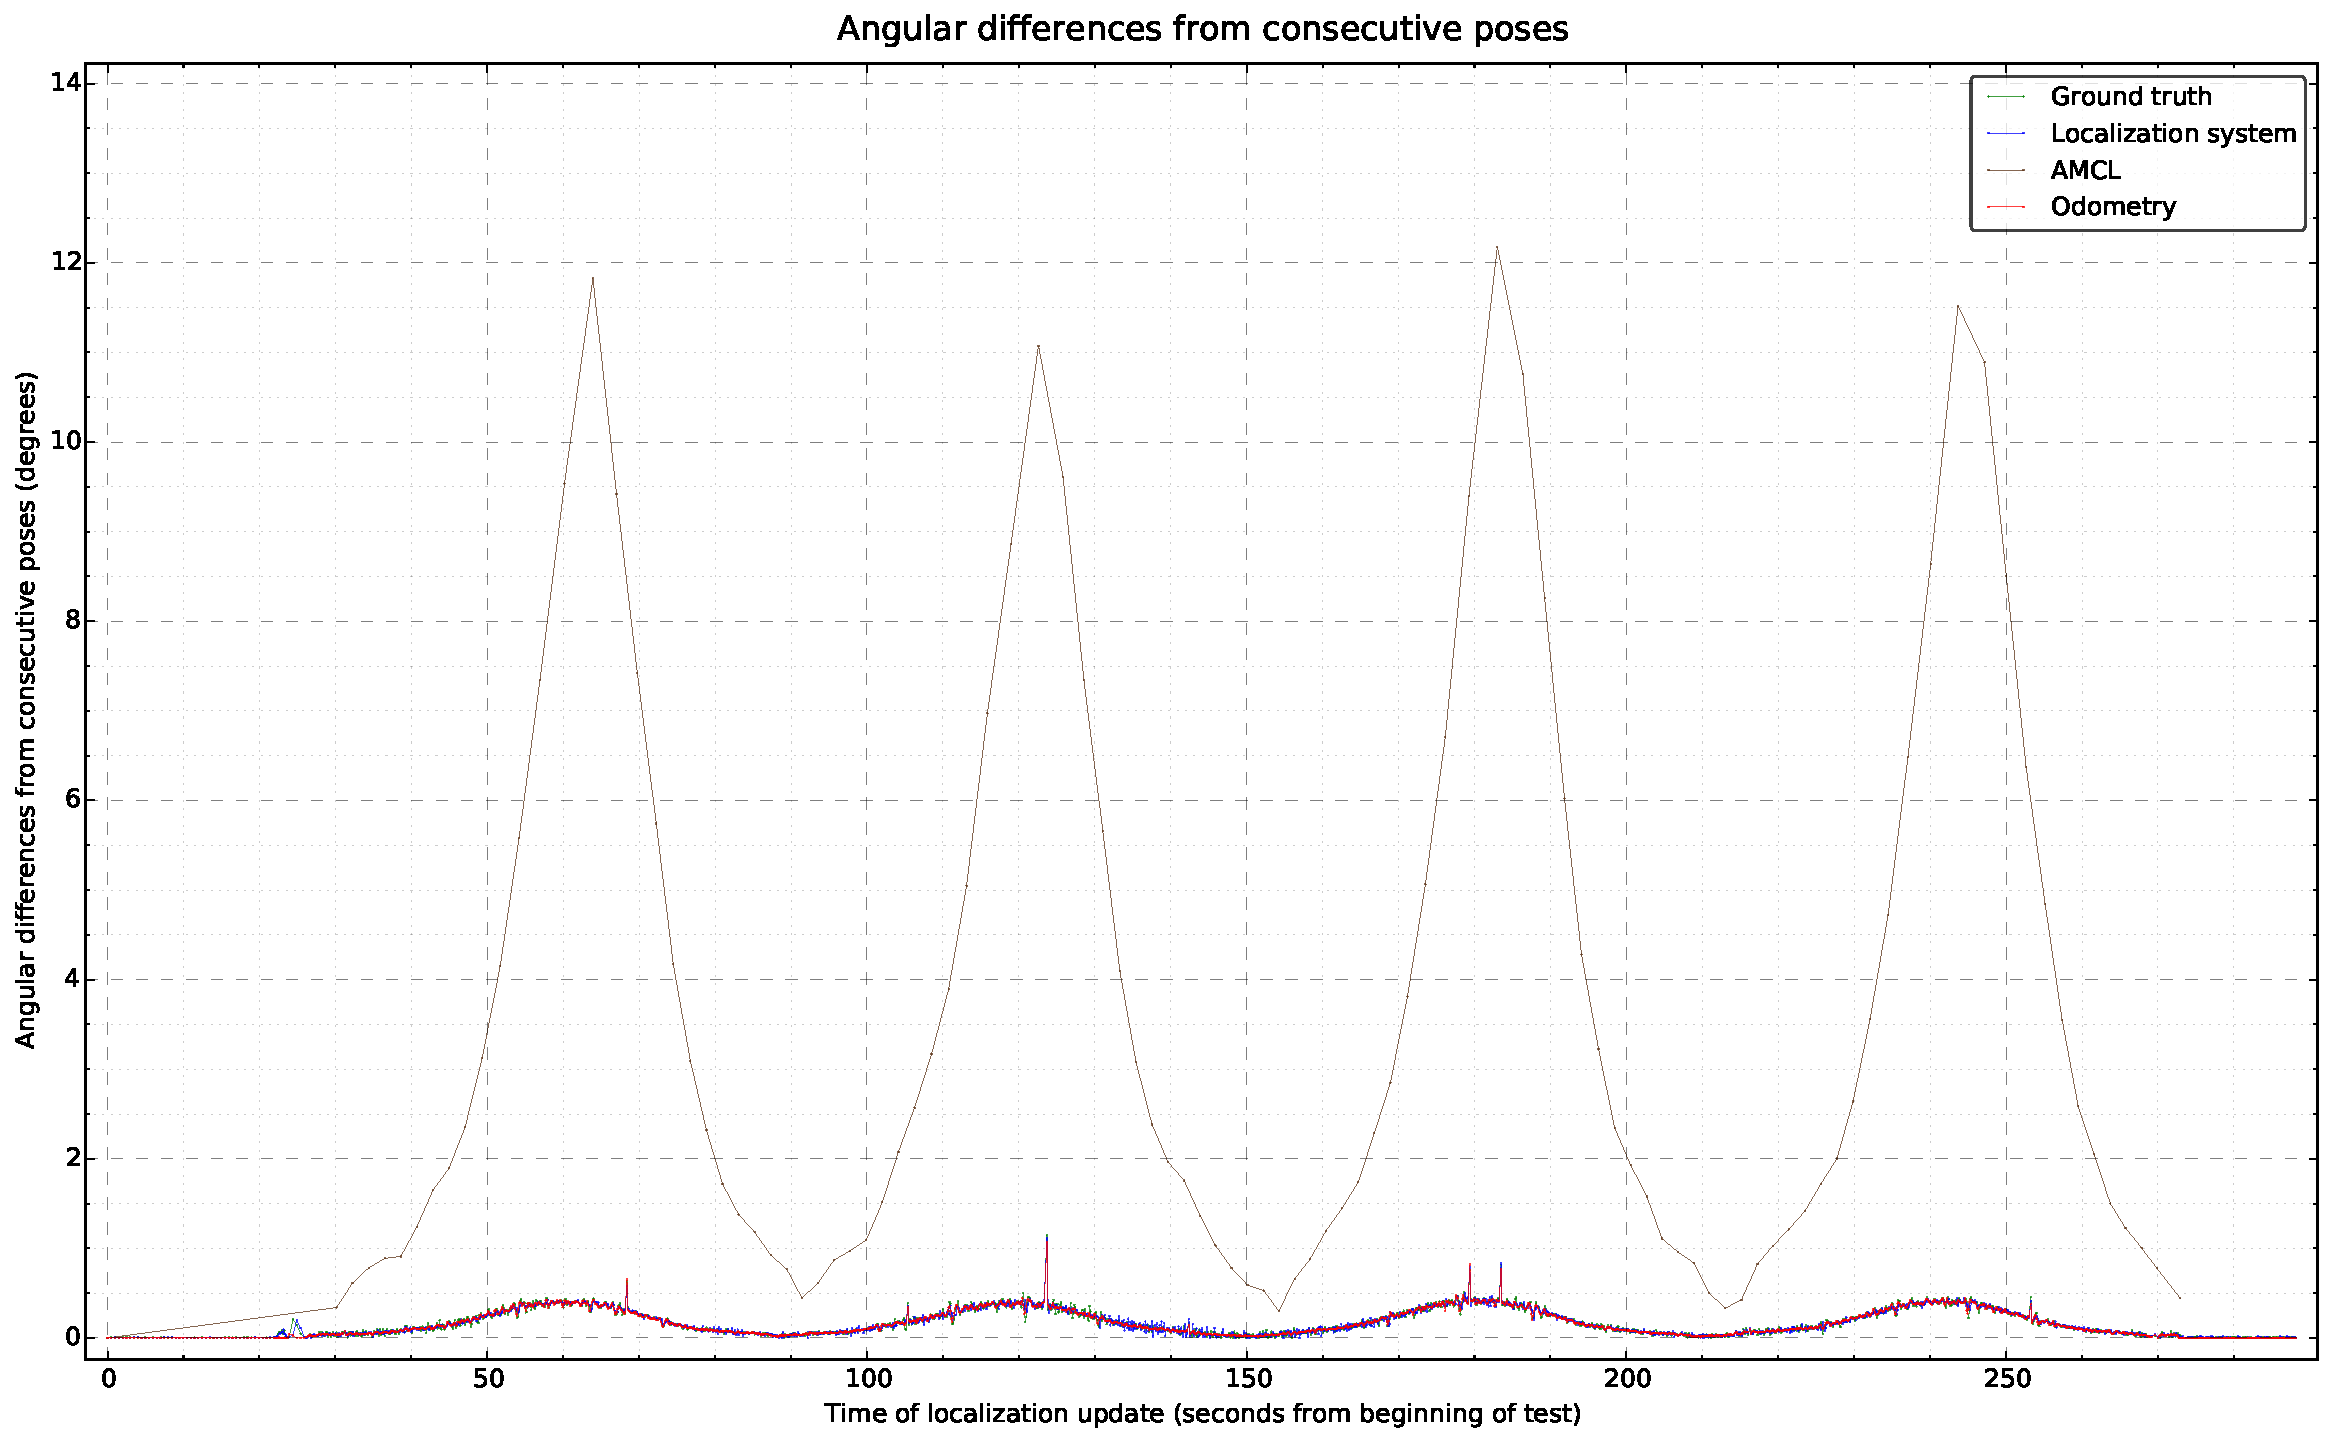
\includegraphics[width=0.69\textwidth]{appendices/tests-3dof/pioneer-robot/\currfilebase/graphs/robot-movement-path-angular-differences-with-amcl}
	\caption{Angular differences between consecutive pose estimations}
\end{figure}

\begin{figure}[H]
	\centering
	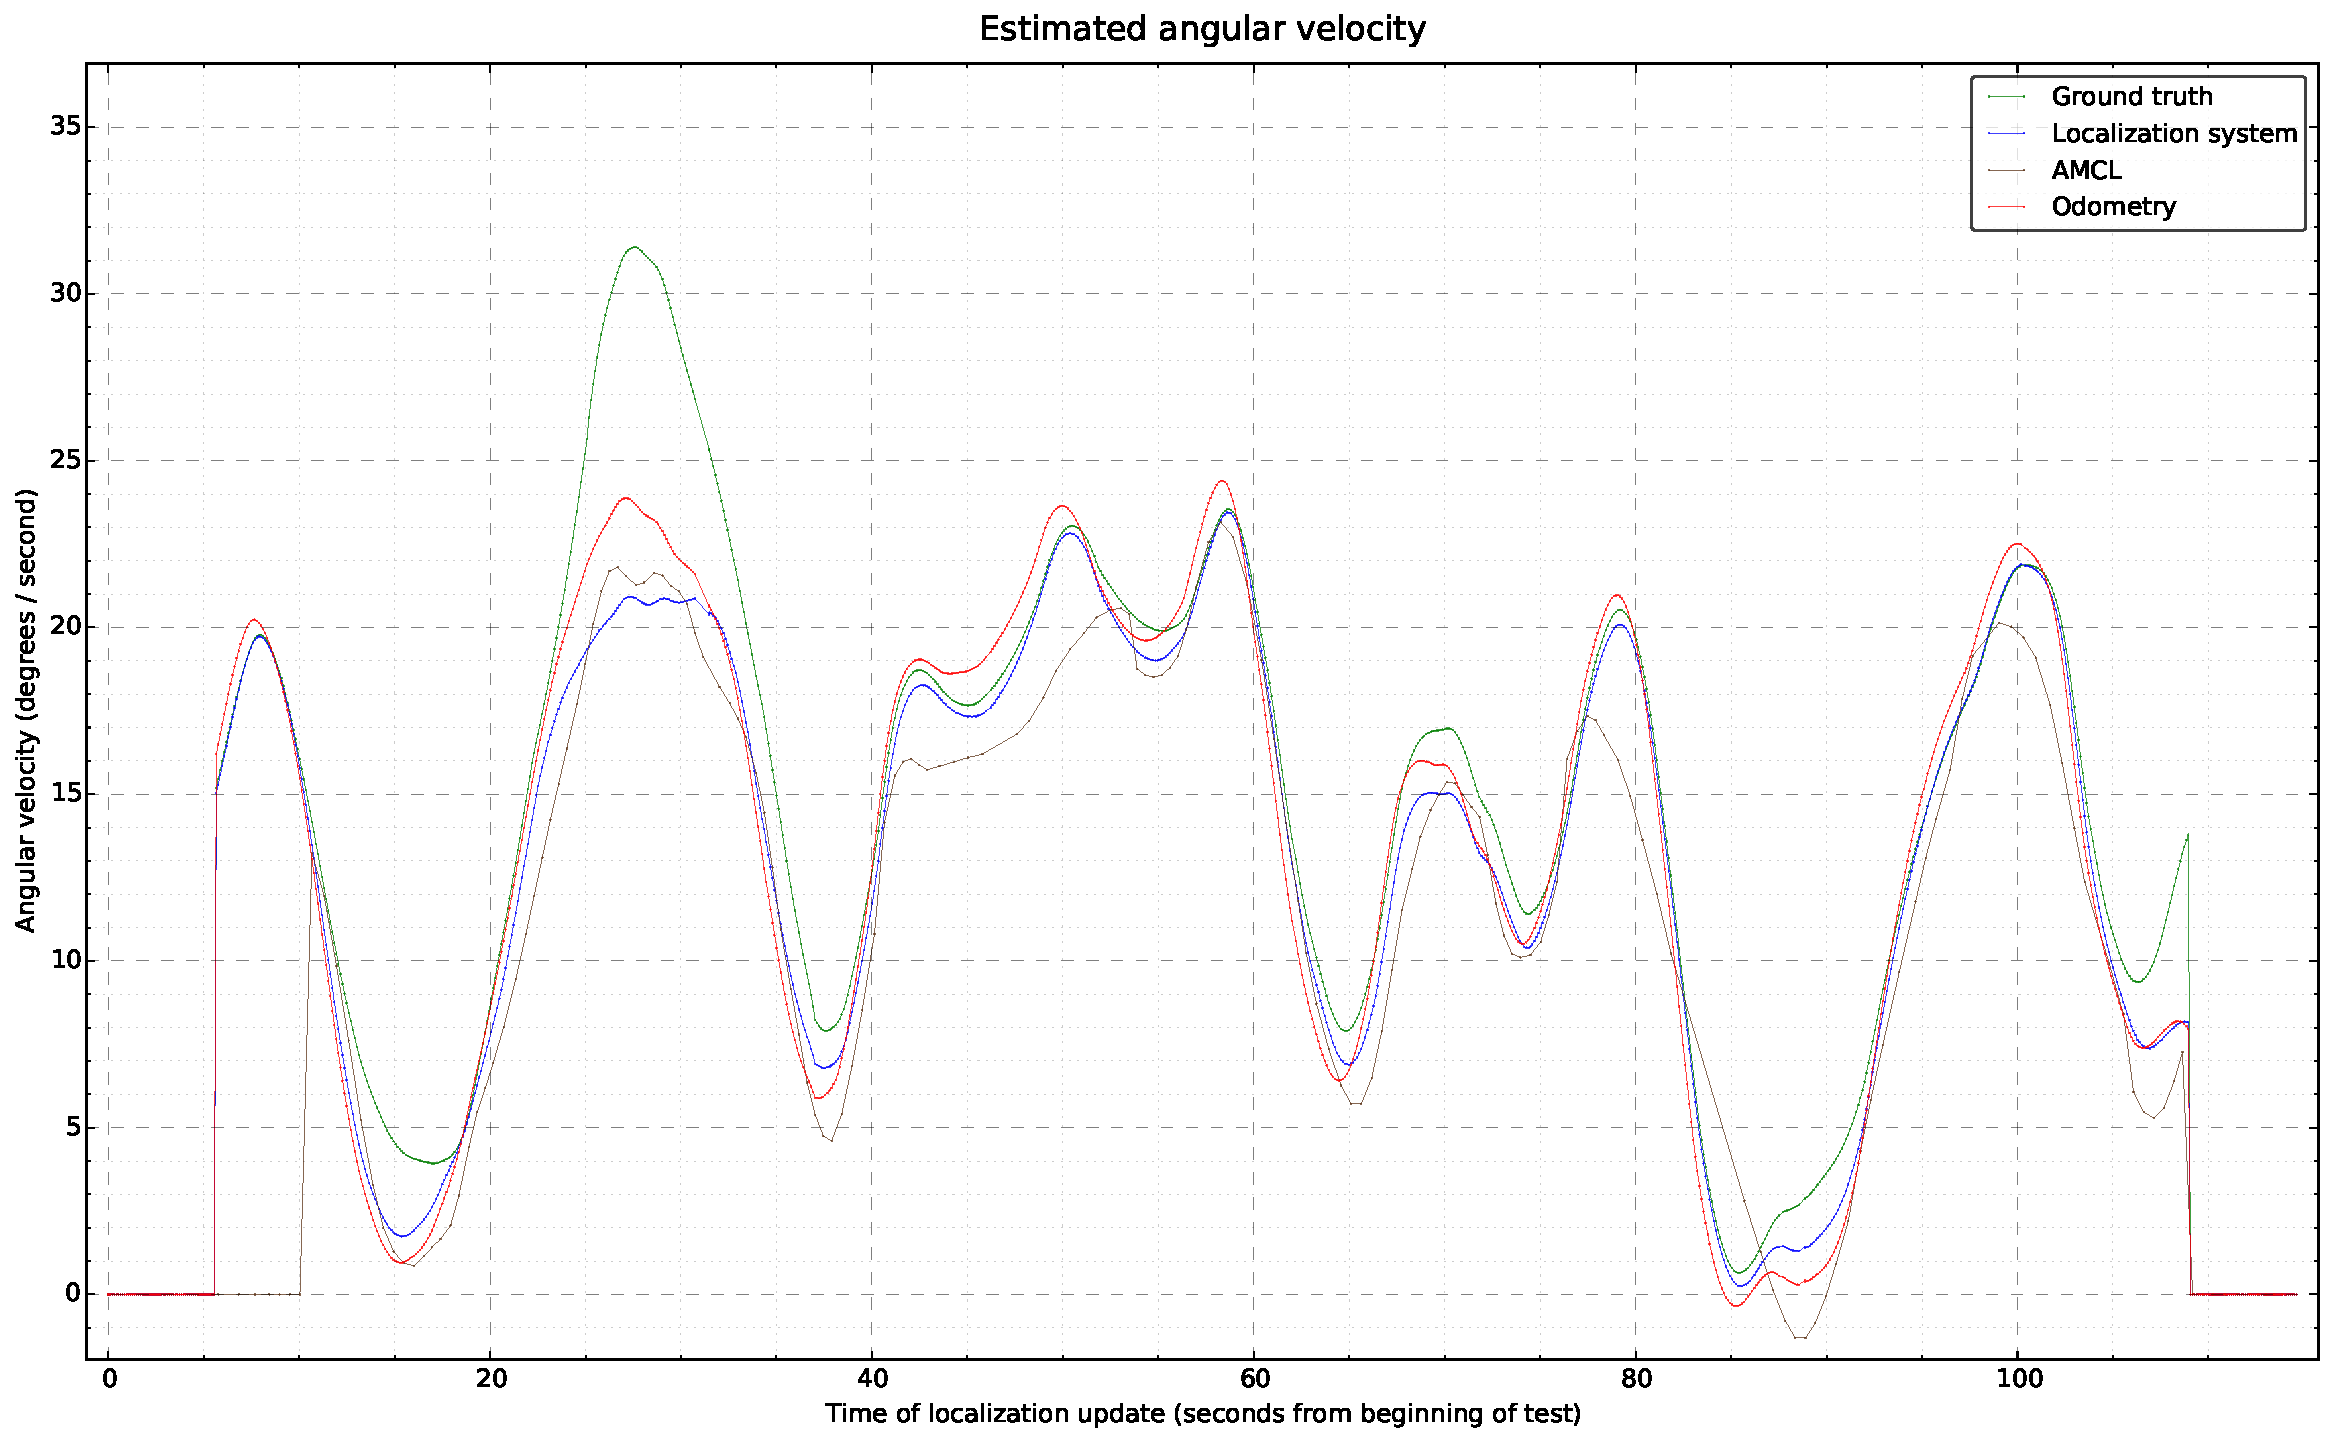
\includegraphics[width=0.69\textwidth]{appendices/tests-3dof/pioneer-robot/\currfilebase/graphs/robot-movement-path-angular-velocity-with-amcl}
	\caption{Estimated angular velocity}
\end{figure}

\begin{figure}[H]
	\centering
	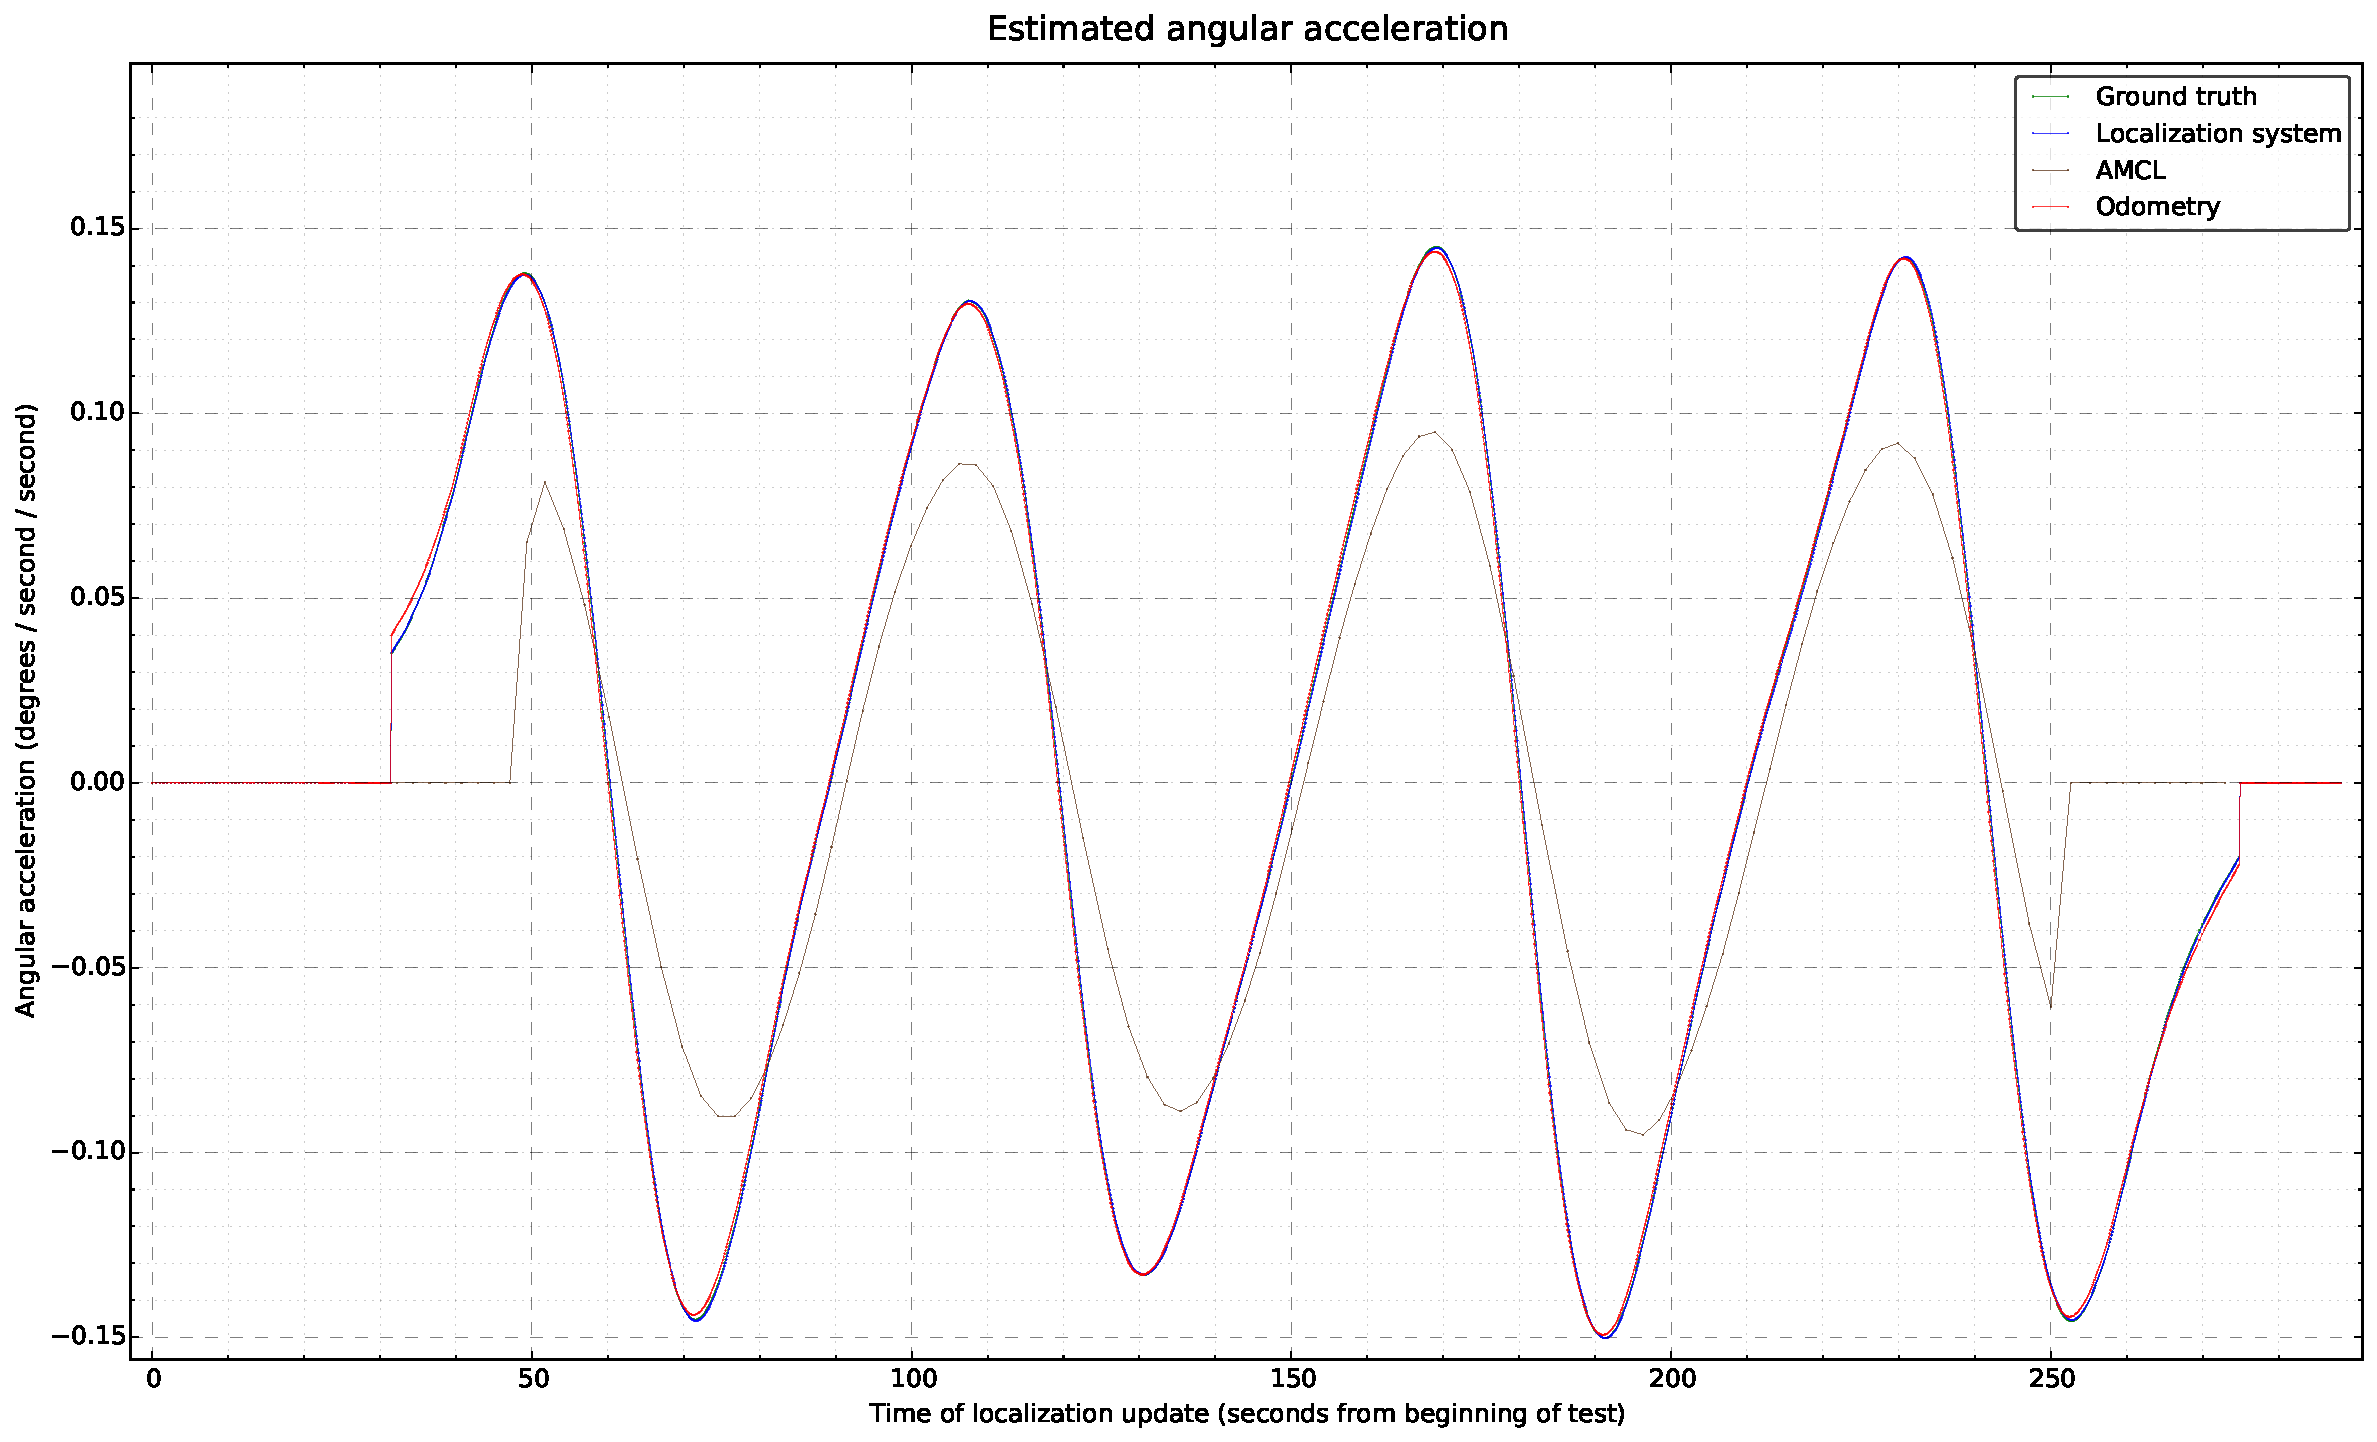
\includegraphics[width=0.69\textwidth]{appendices/tests-3dof/pioneer-robot/\currfilebase/graphs/robot-movement-path-angular-acceleration-with-amcl}
	\caption{Estimated angular acceleration}
\end{figure}


%Translation errors
\begin{figure}[H]
	\centering
	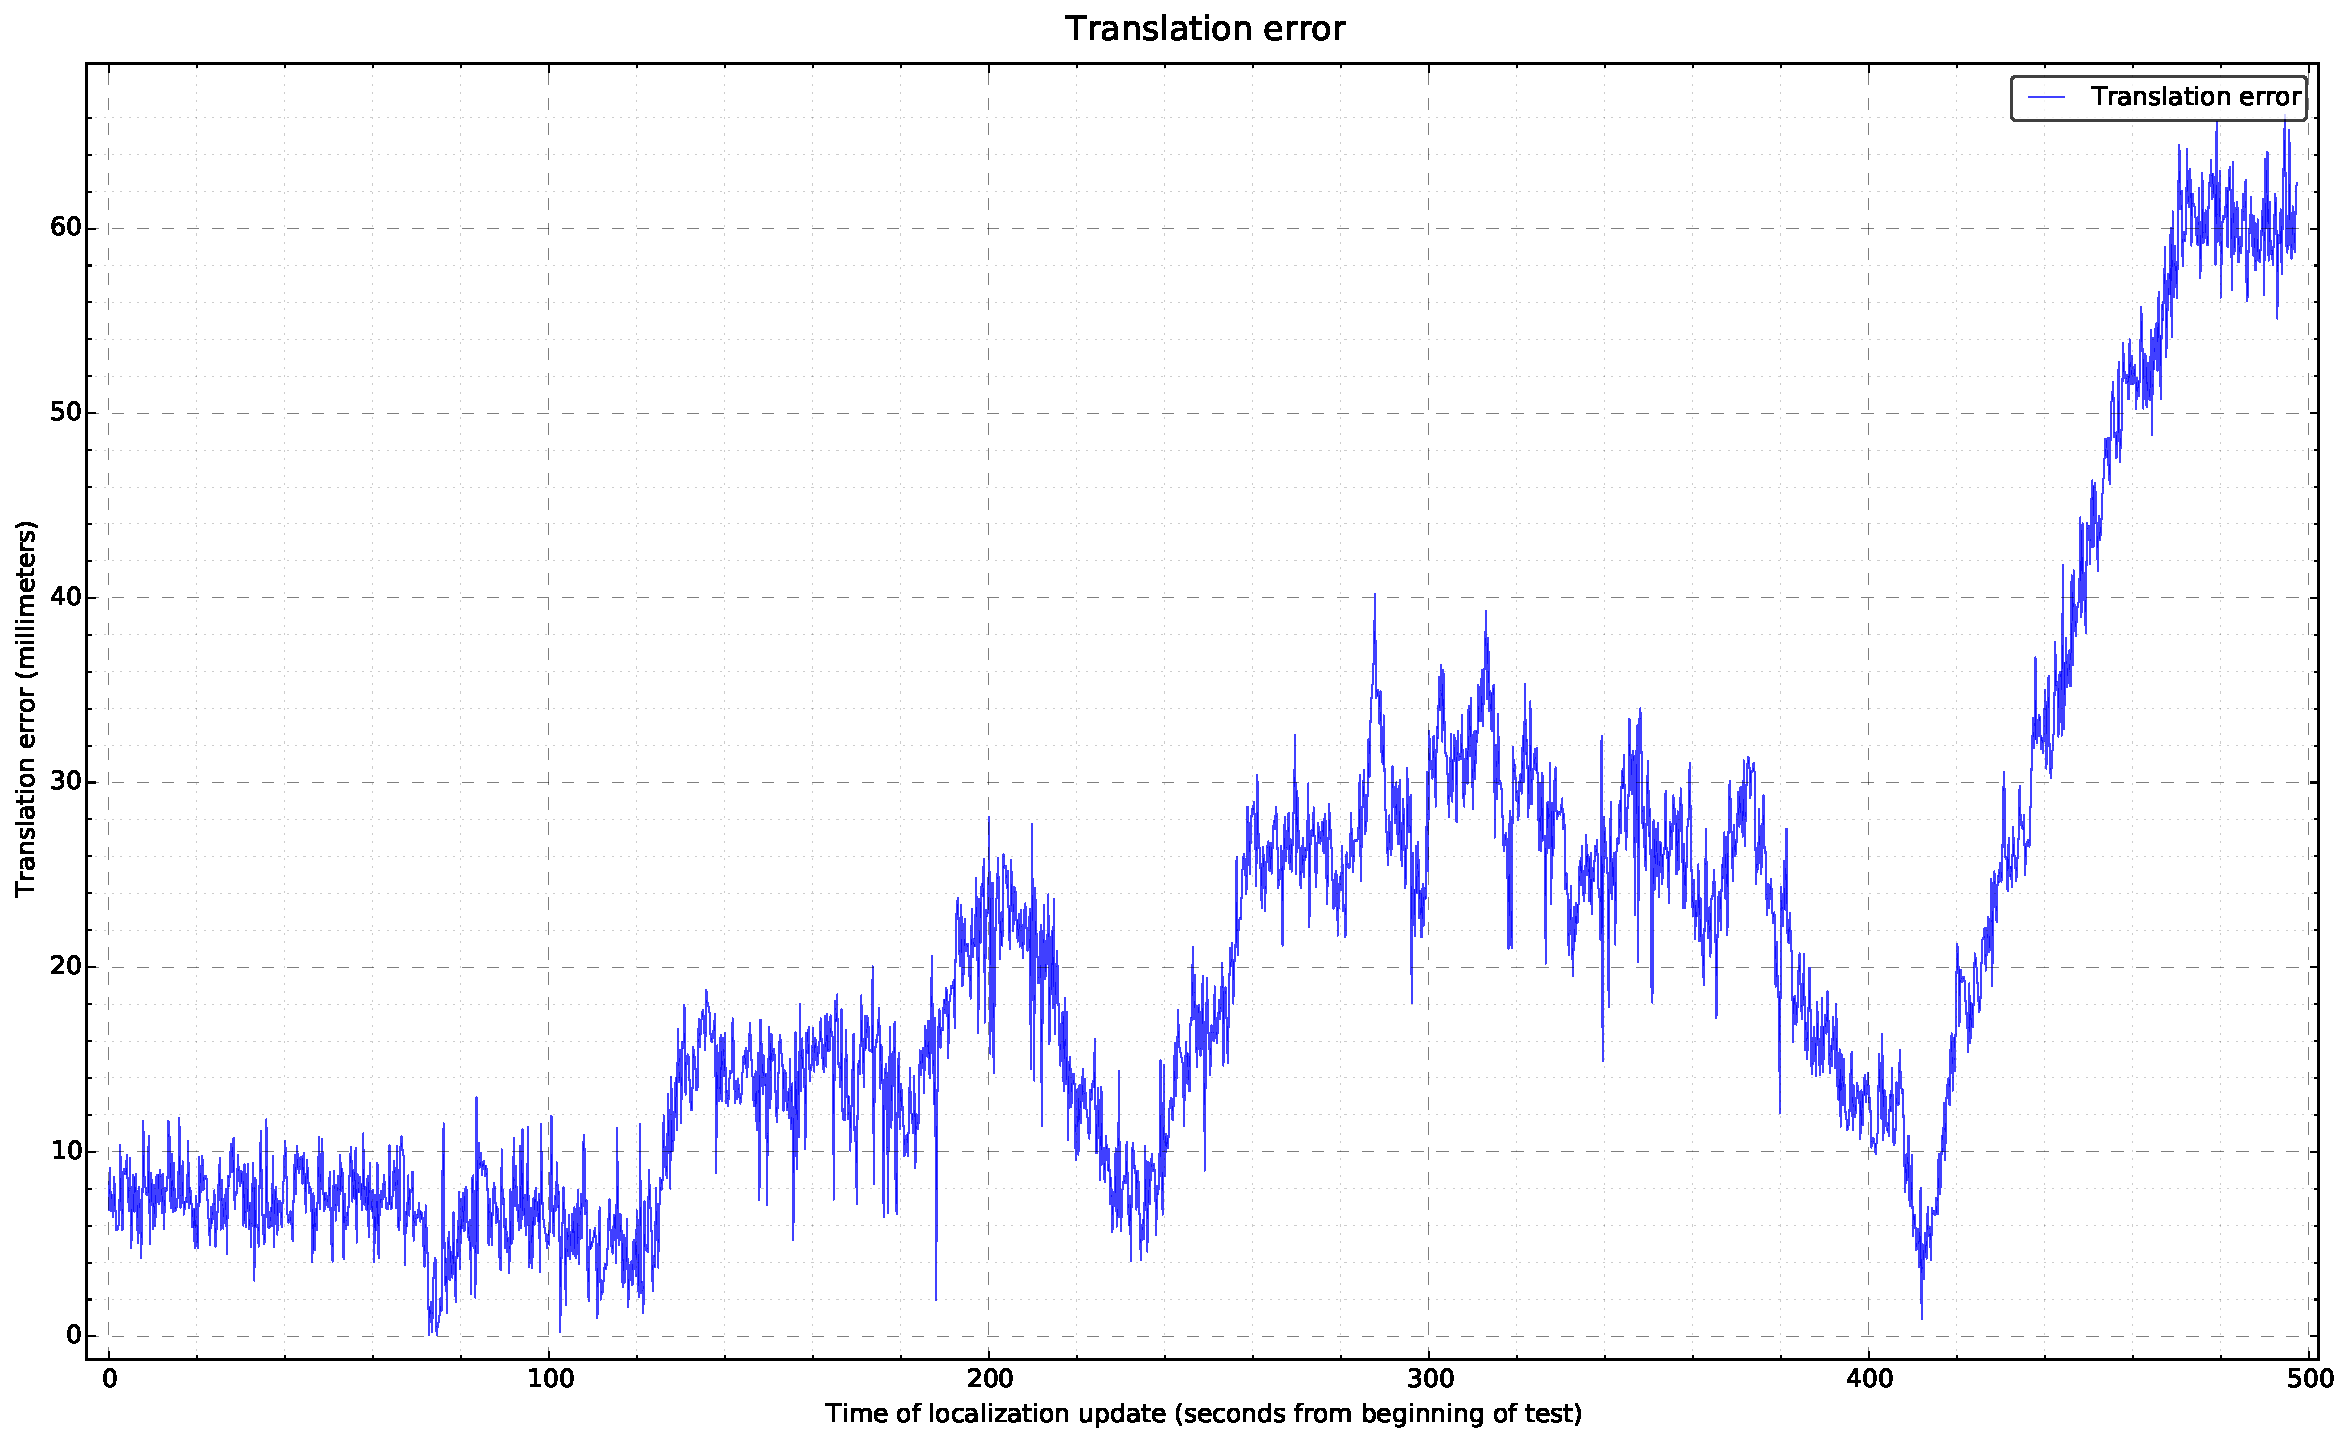
\includegraphics[width=0.69\textwidth]{appendices/tests-3dof/pioneer-robot/\currfilebase/graphs/odometry-translation-error-millimeters}
	\caption{Odometry translation errors}
\end{figure}

\begin{figure}[H]
	\centering
	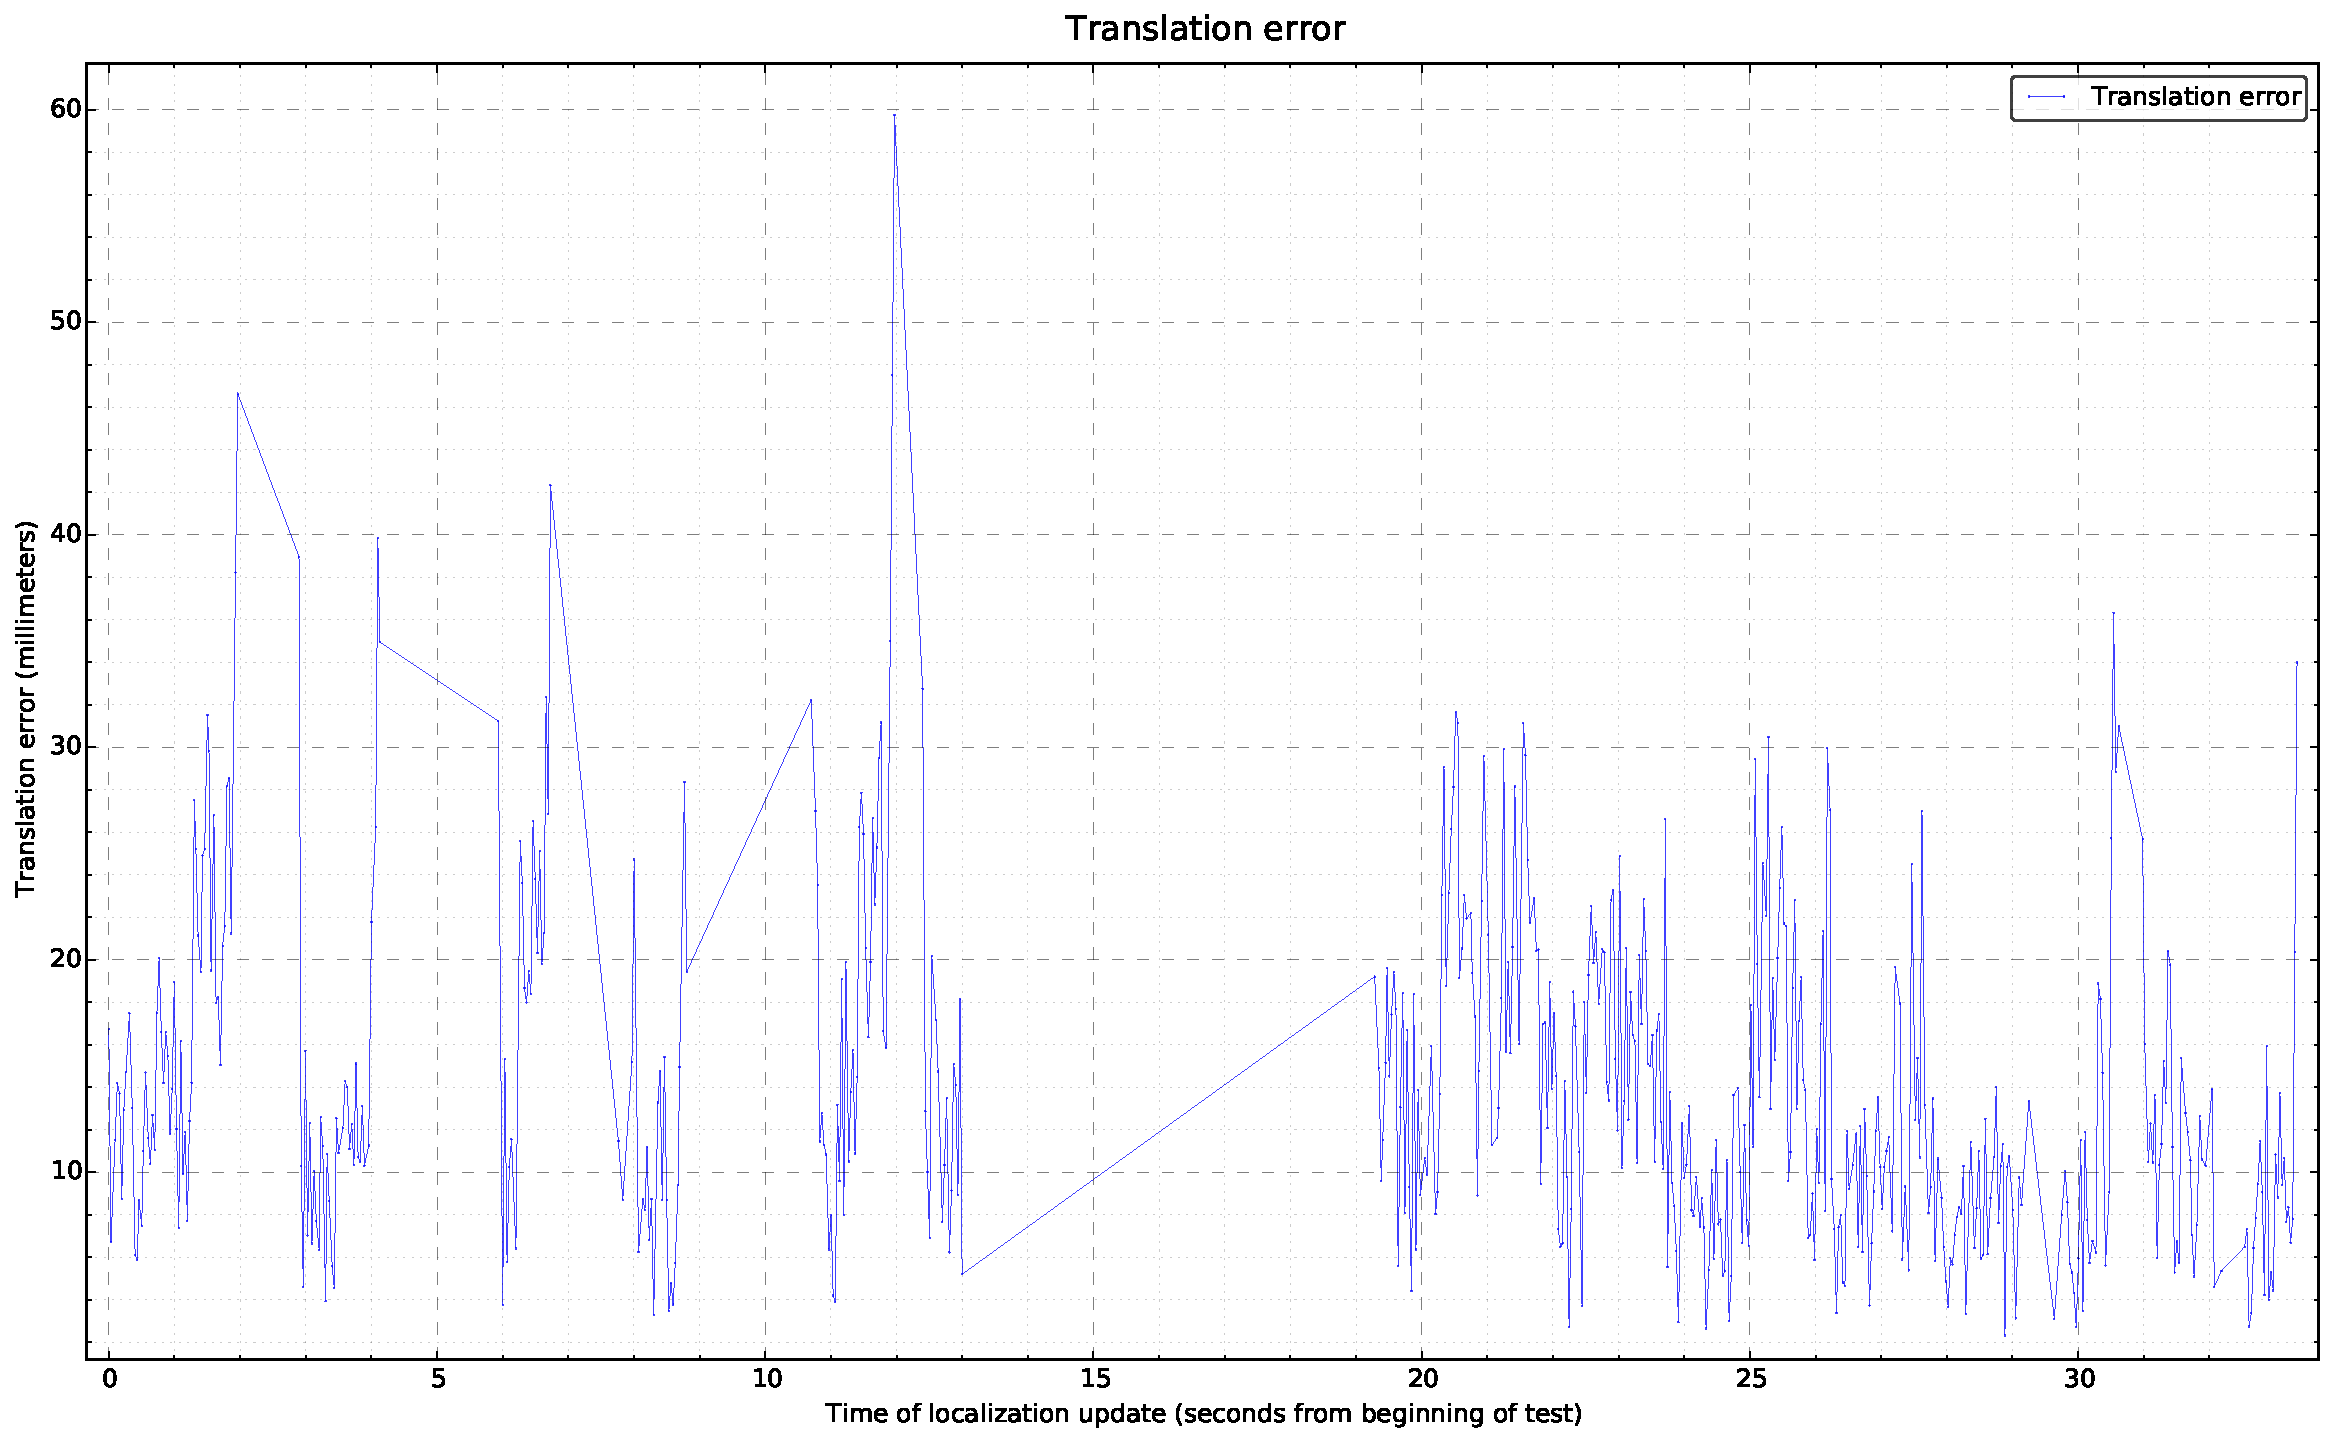
\includegraphics[width=0.69\textwidth]{appendices/tests-3dof/pioneer-robot/\currfilebase/graphs/translation-error-millimeters}
	\caption{Localization system translation errors}
\end{figure}

\begin{figure}[H]
	\centering
	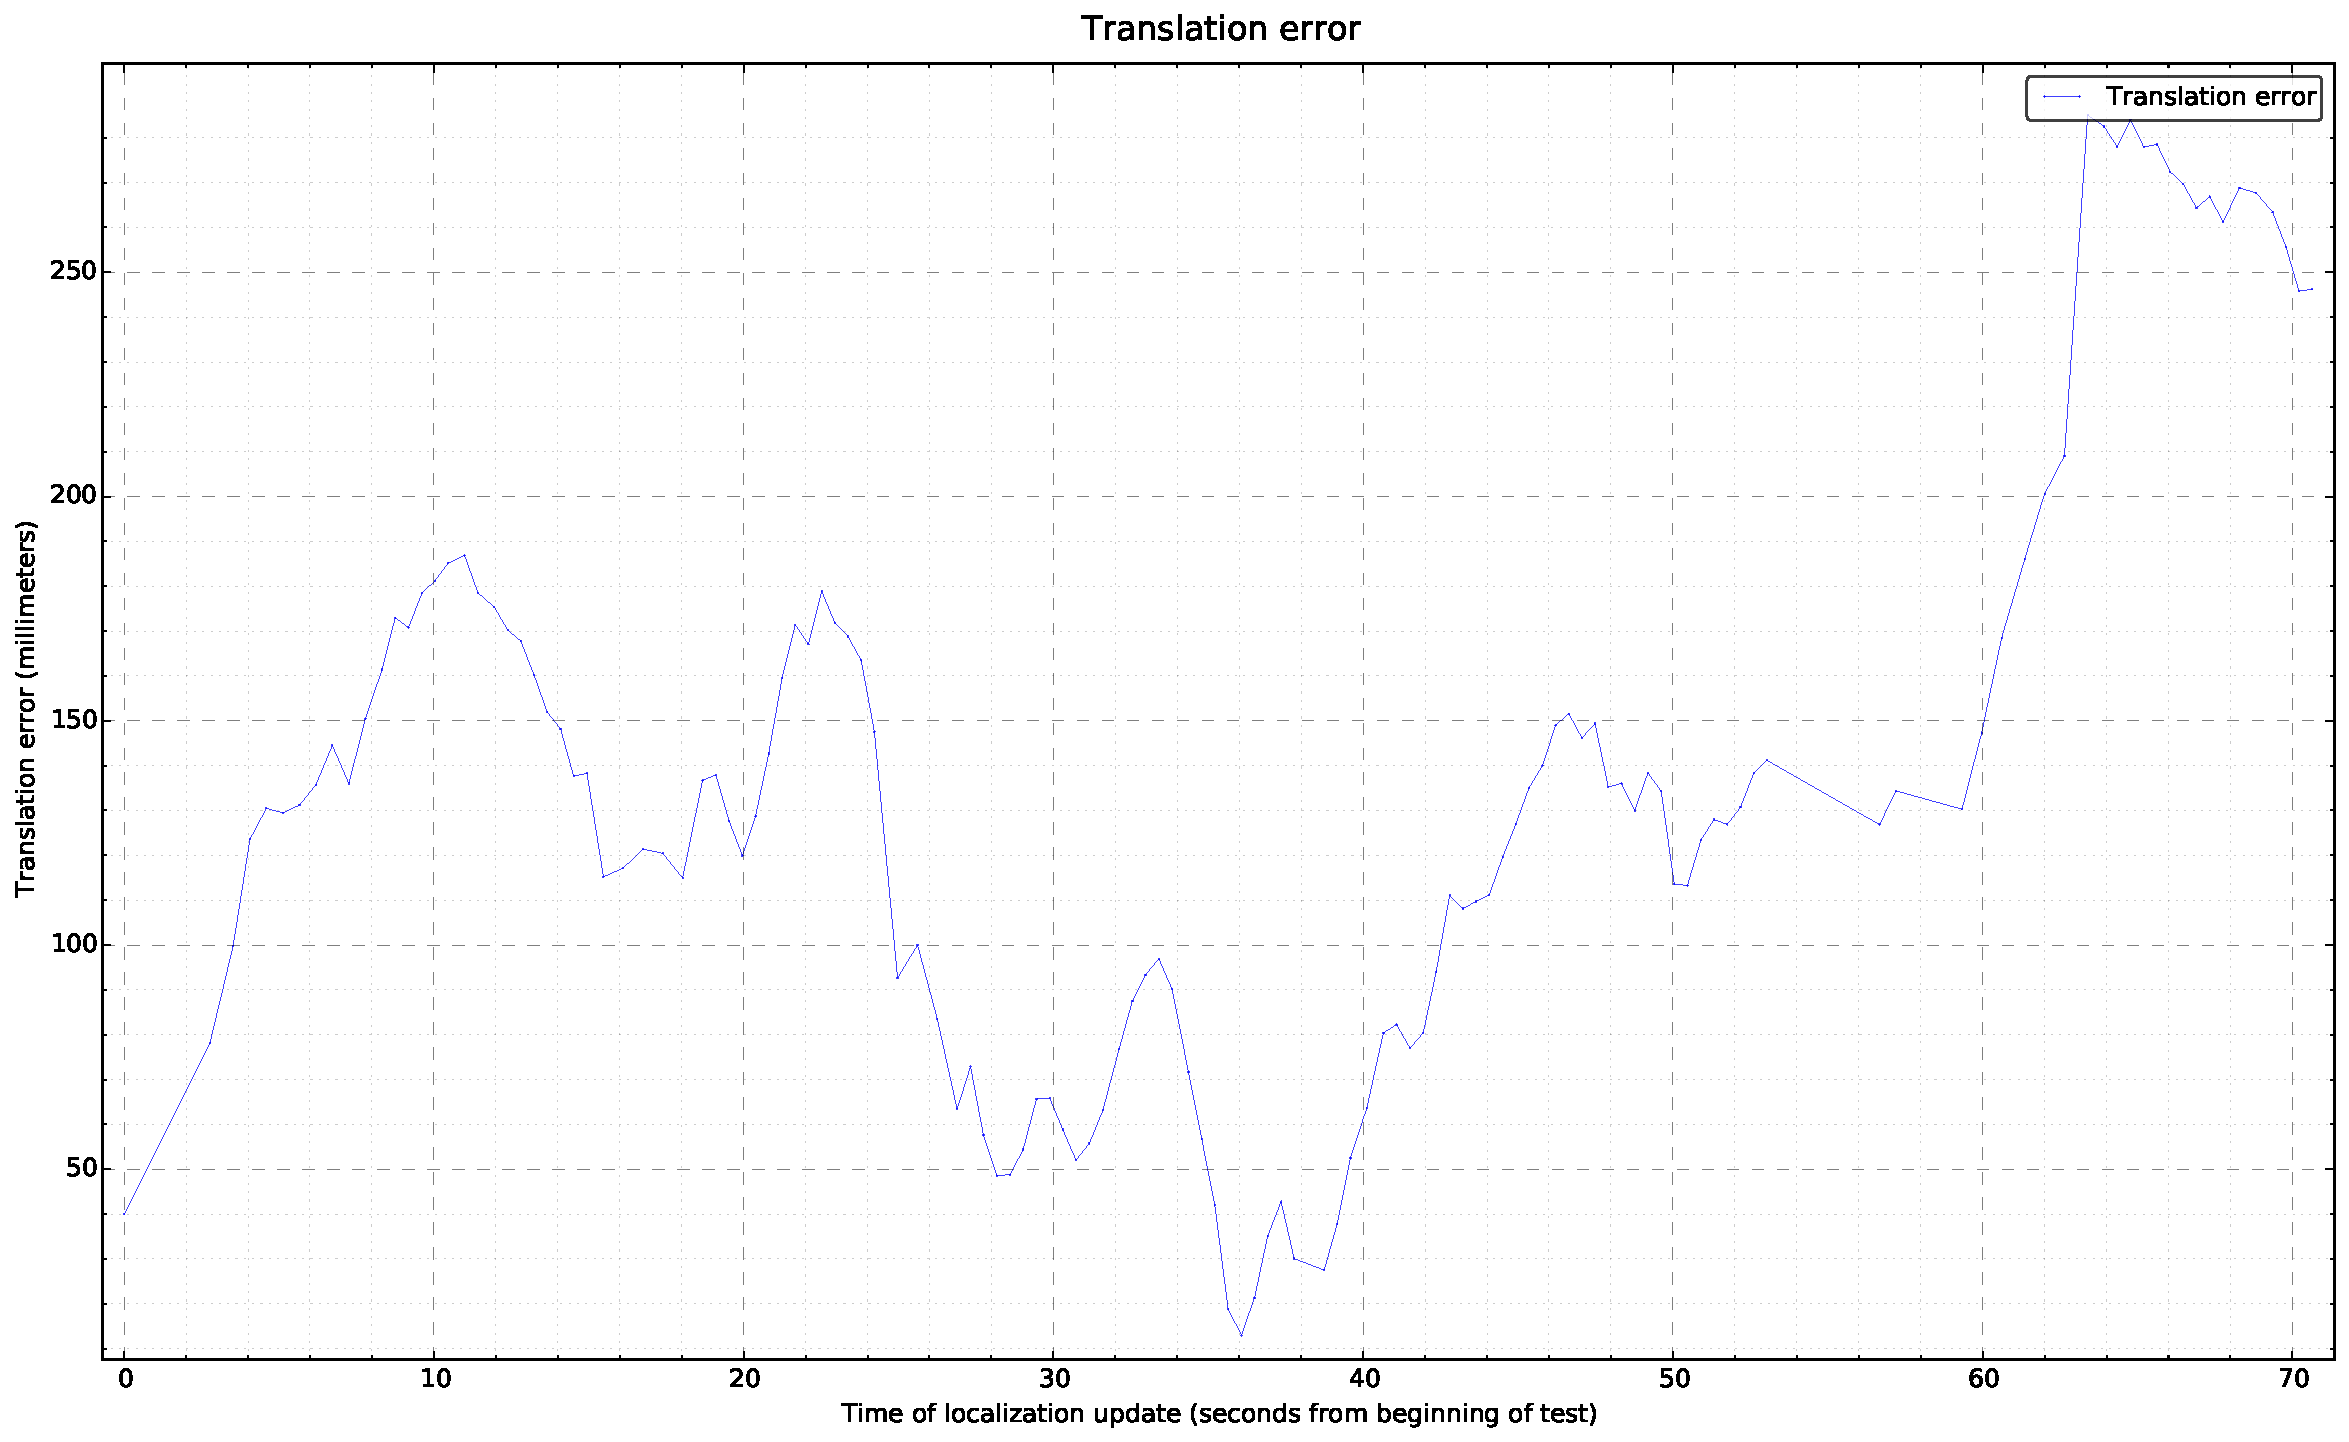
\includegraphics[width=0.69\textwidth]{appendices/tests-3dof/pioneer-robot/\currfilebase/graphs/translation-error-millimeters-amcl}
	\caption{\glsentrytext{amcl} translation errors}
\end{figure}


%Translation errors components
\begin{figure}[H]
	\centering
	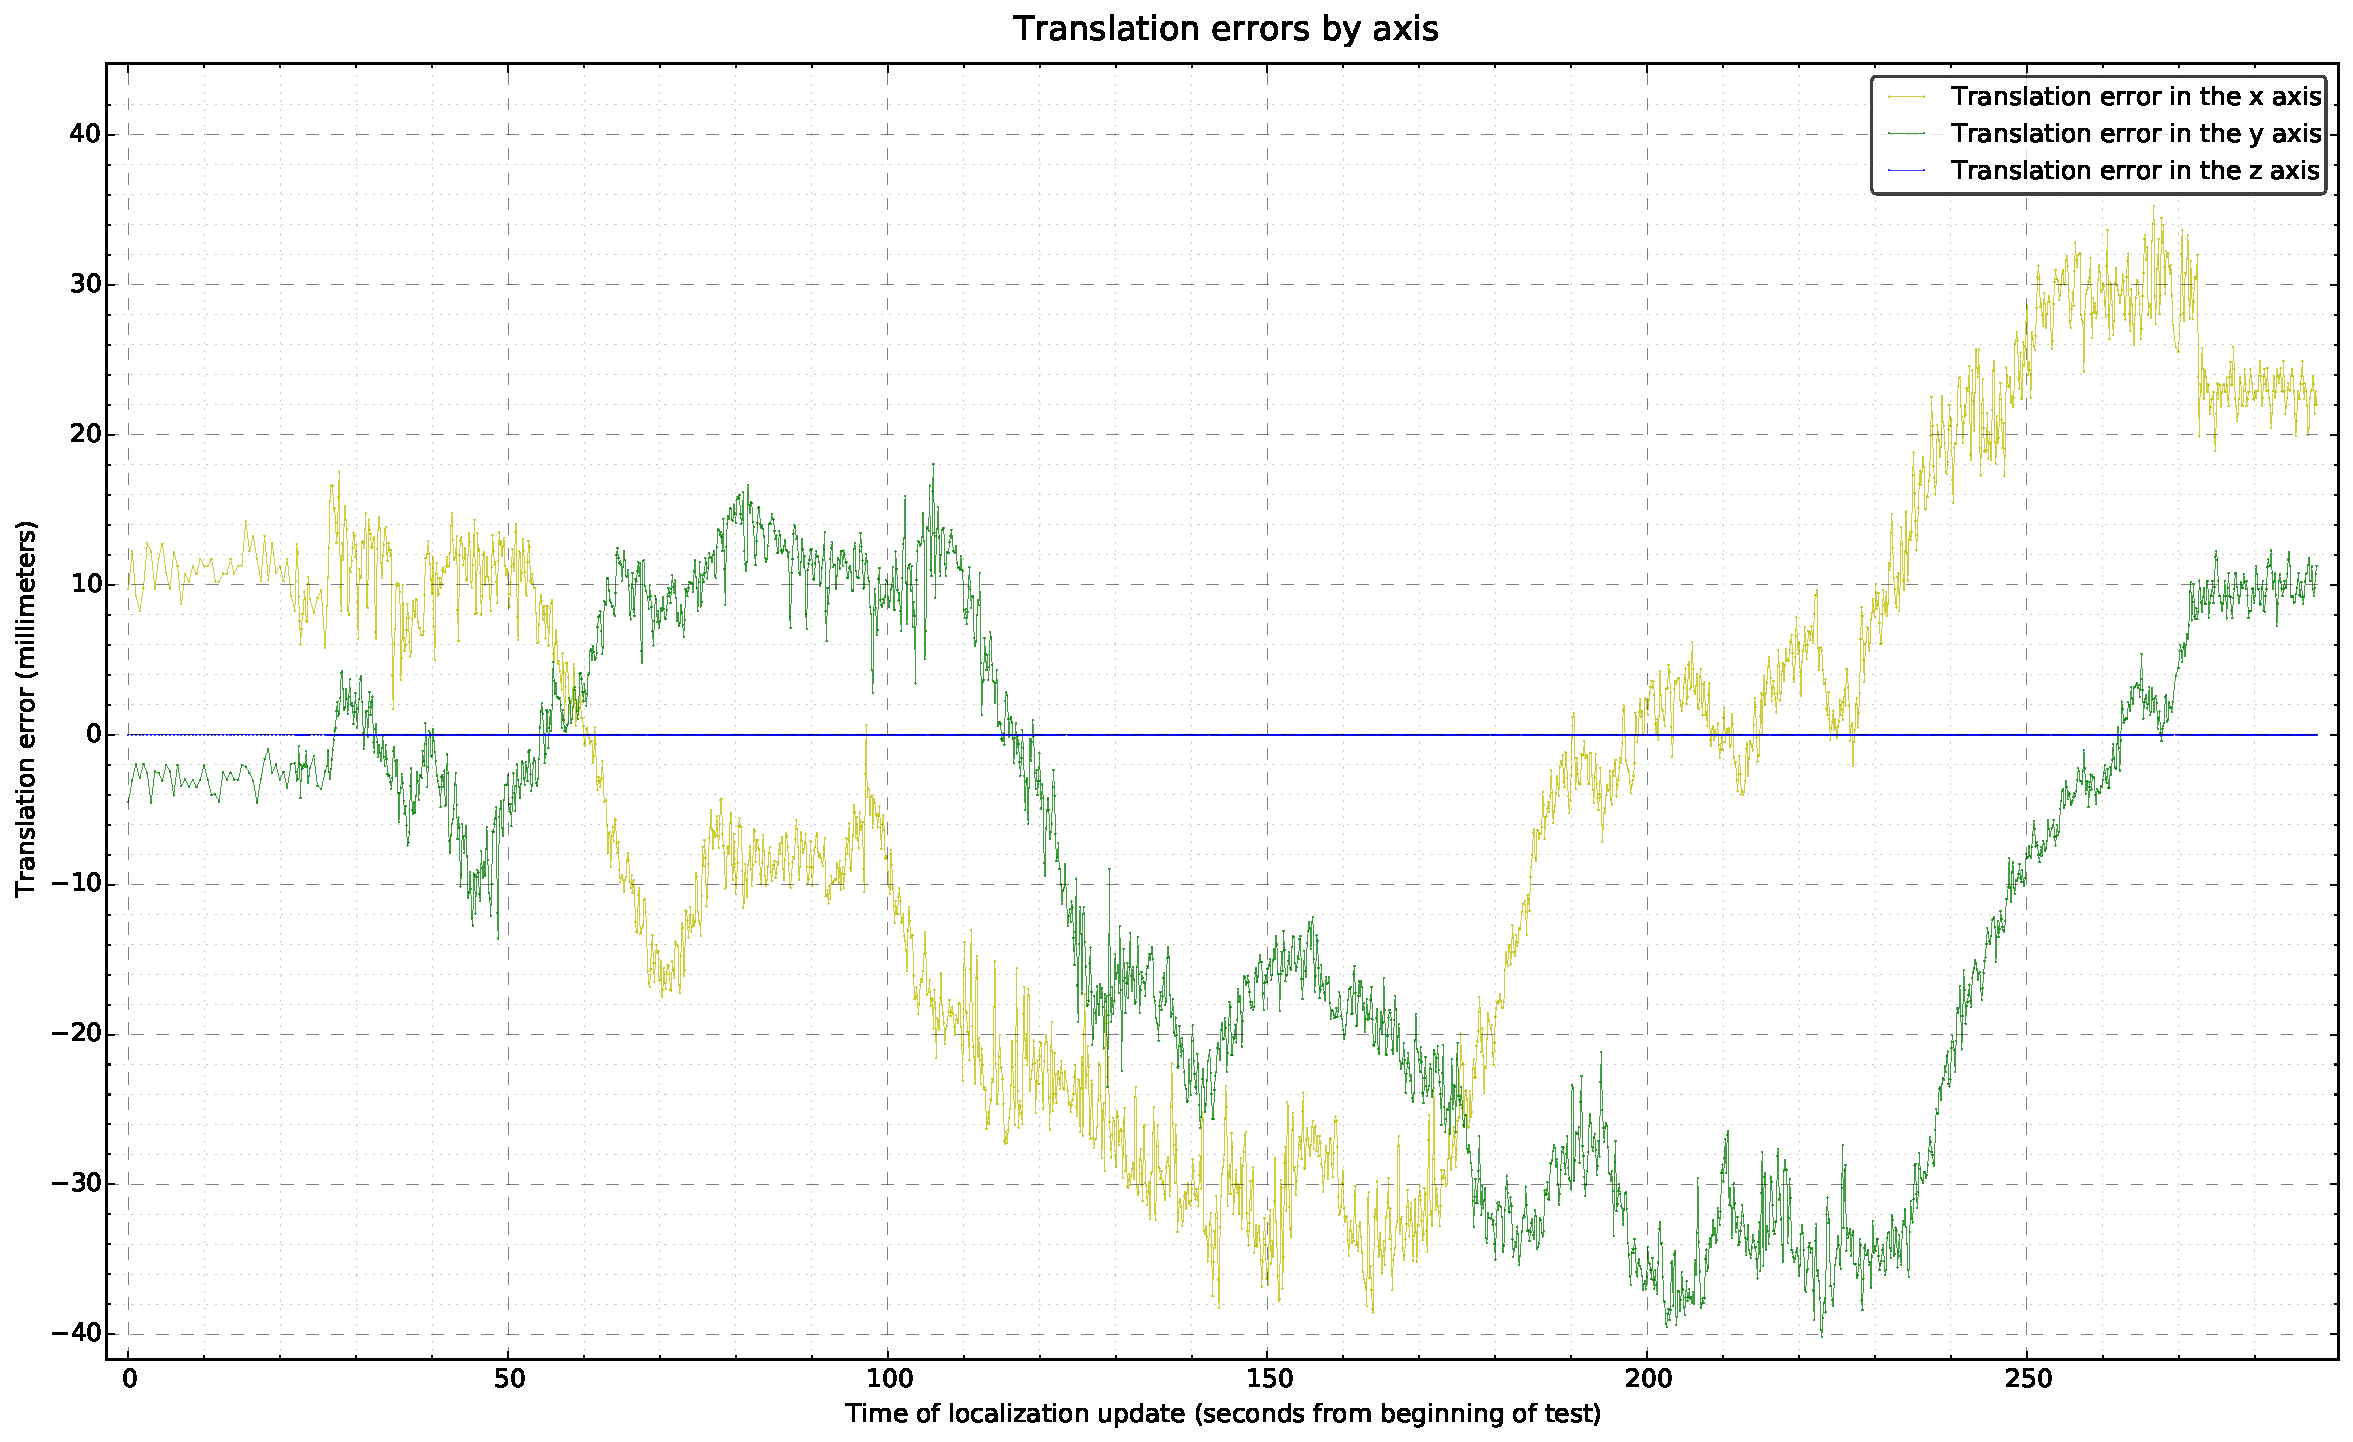
\includegraphics[width=0.69\textwidth]{appendices/tests-3dof/pioneer-robot/\currfilebase/graphs/odometry-translation-error-components-millimeters}
	\caption{Odometry translation errors components}
\end{figure}

\begin{figure}[H]
	\centering
	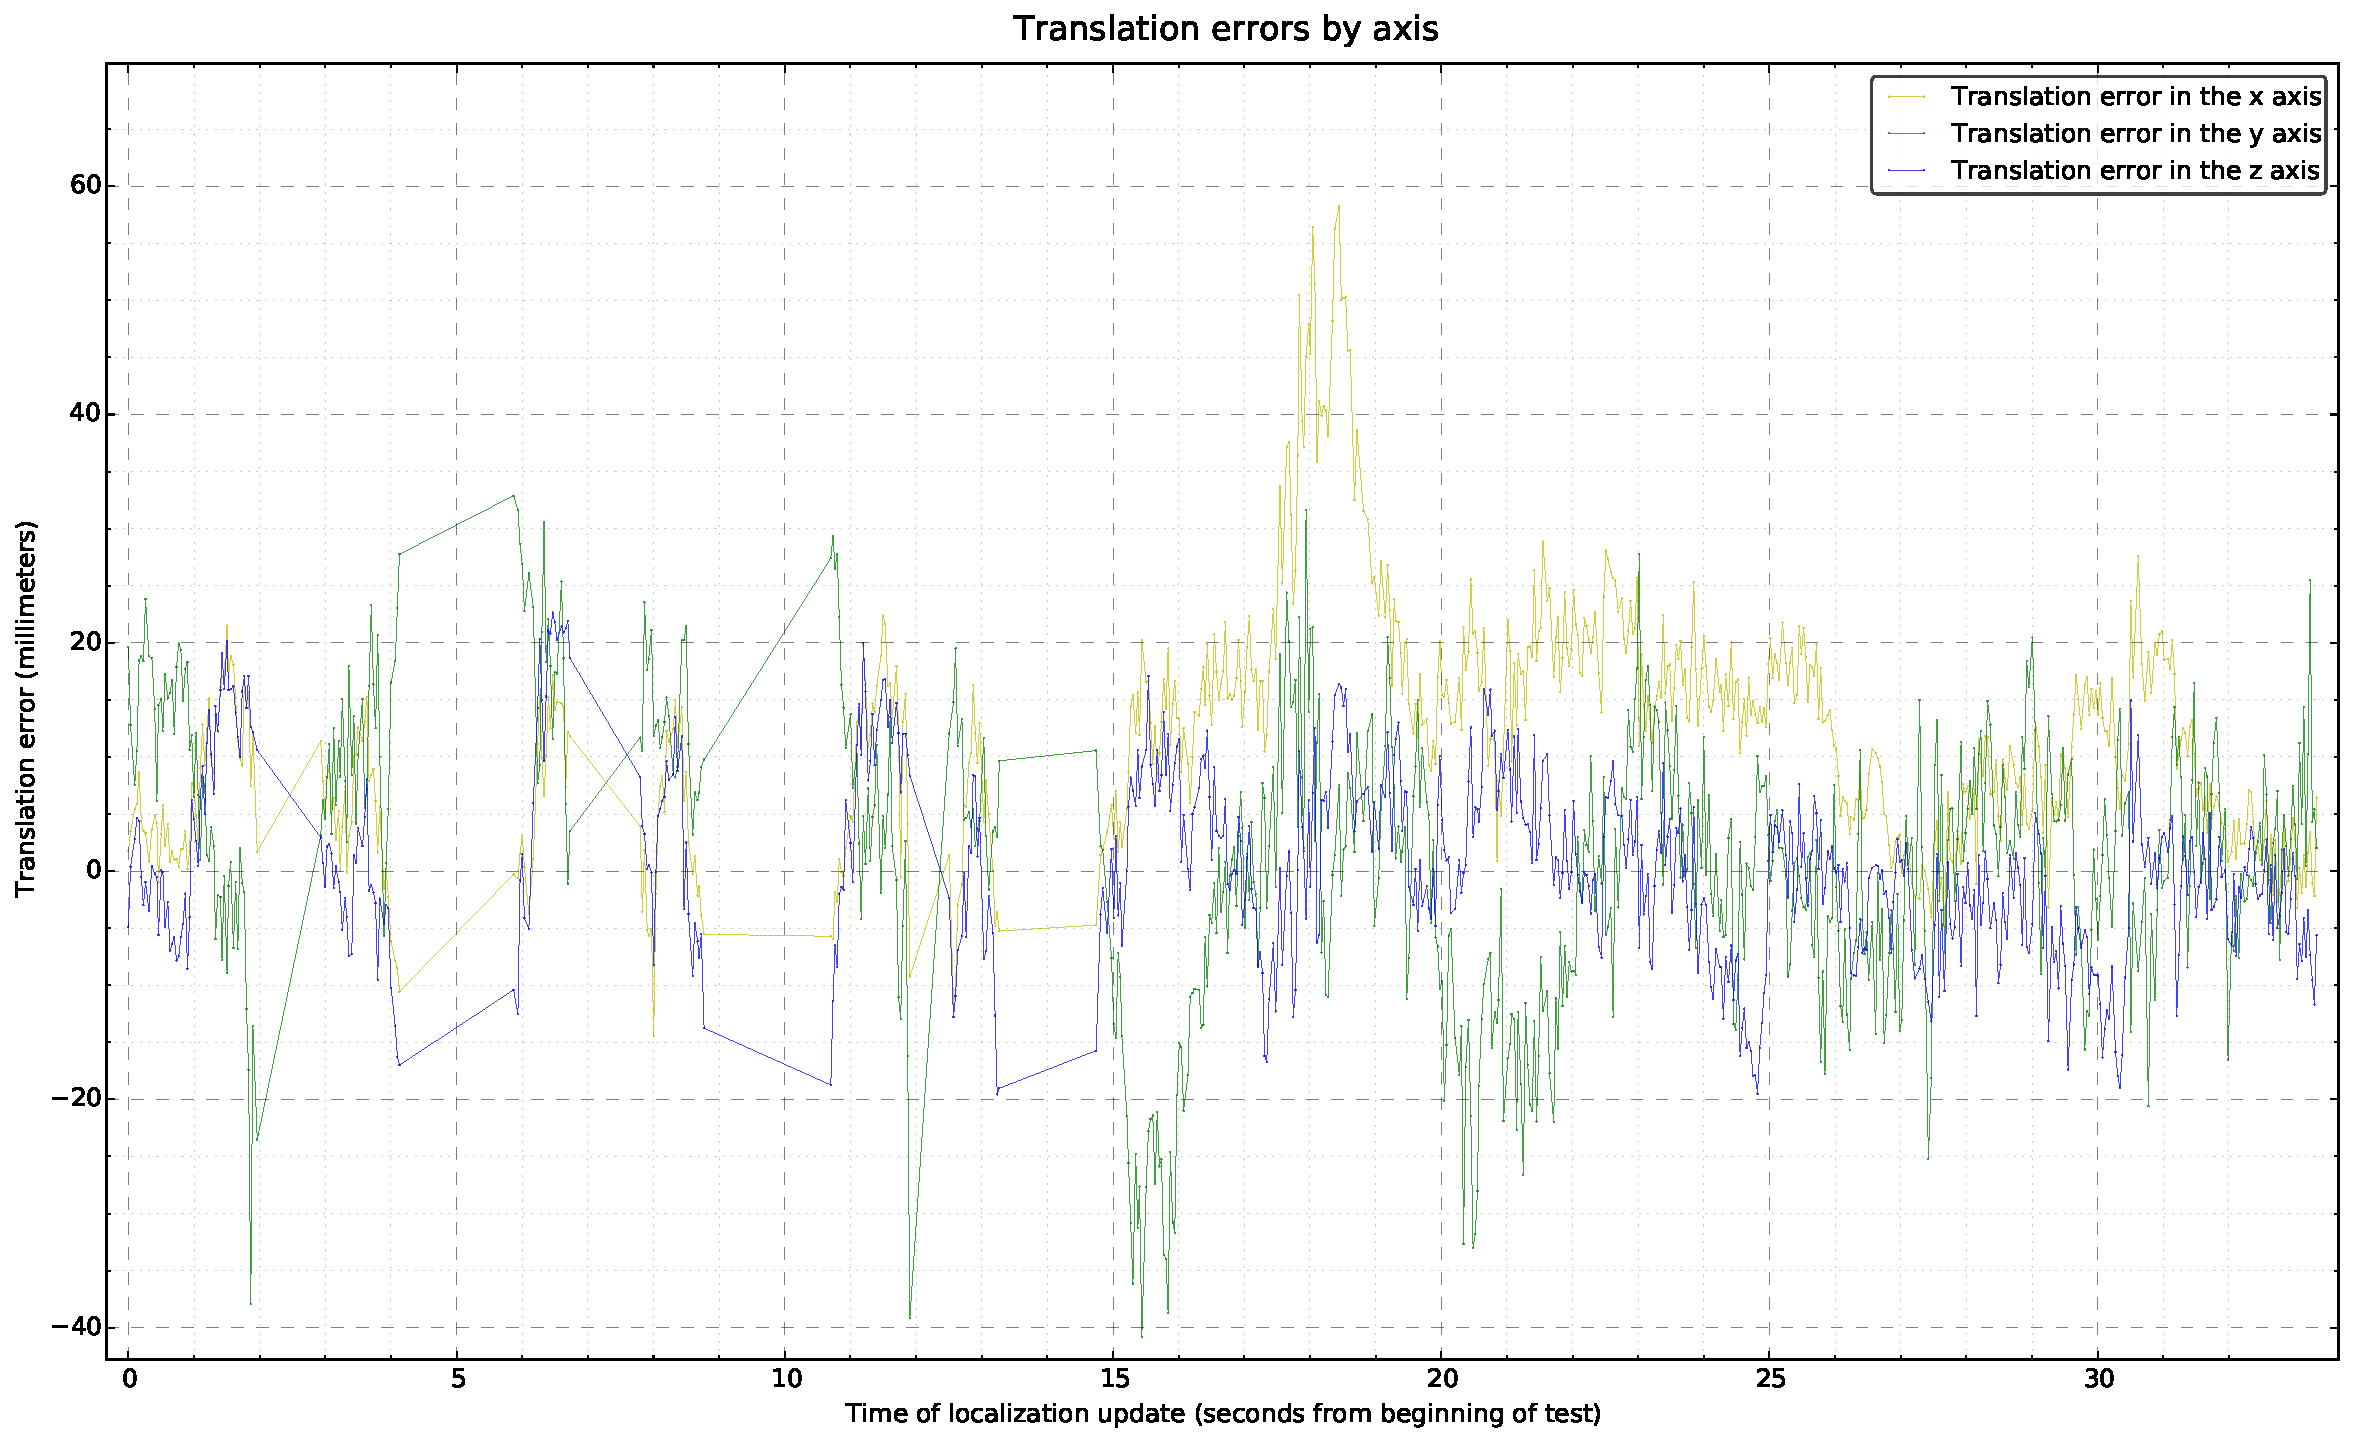
\includegraphics[width=0.69\textwidth]{appendices/tests-3dof/pioneer-robot/\currfilebase/graphs/translation-error-components-millimeters}
	\caption{Localization system translation errors components}
\end{figure}

\begin{figure}[H]
	\centering
	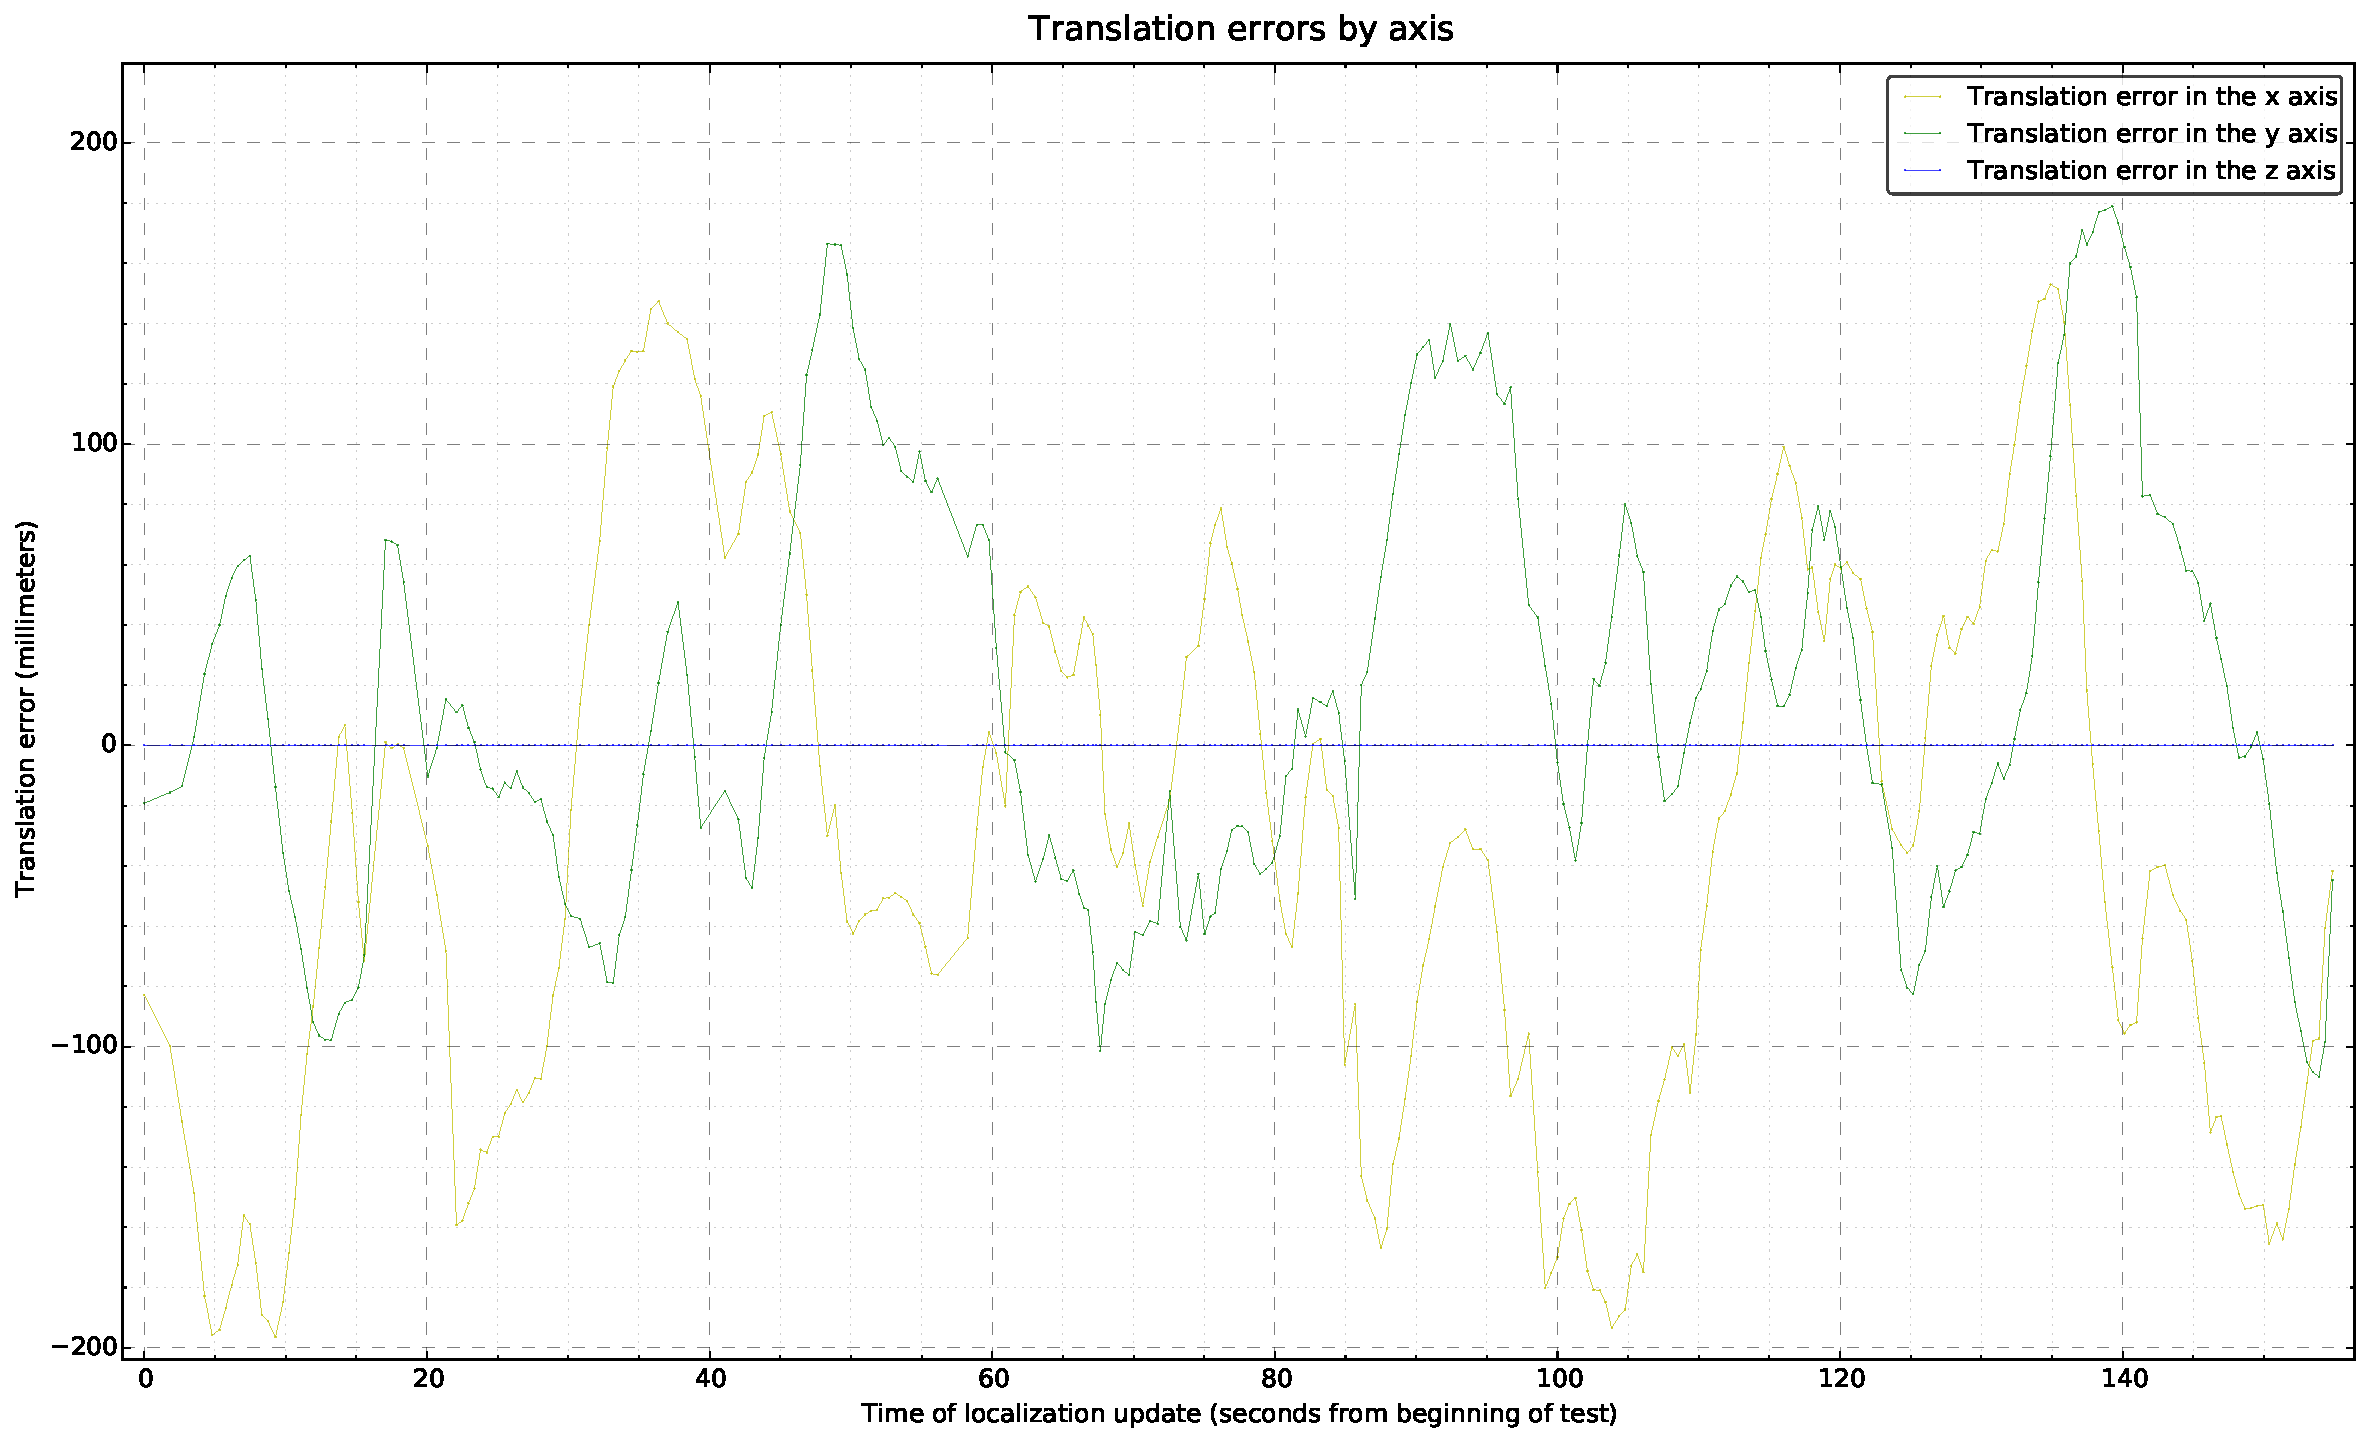
\includegraphics[width=0.69\textwidth]{appendices/tests-3dof/pioneer-robot/\currfilebase/graphs/translation-error-components-millimeters-amcl}
	\caption{\glsentrytext{amcl} translation errors components}
\end{figure}


%Translation errors distributions
\begin{figure}[H]
	\centering
	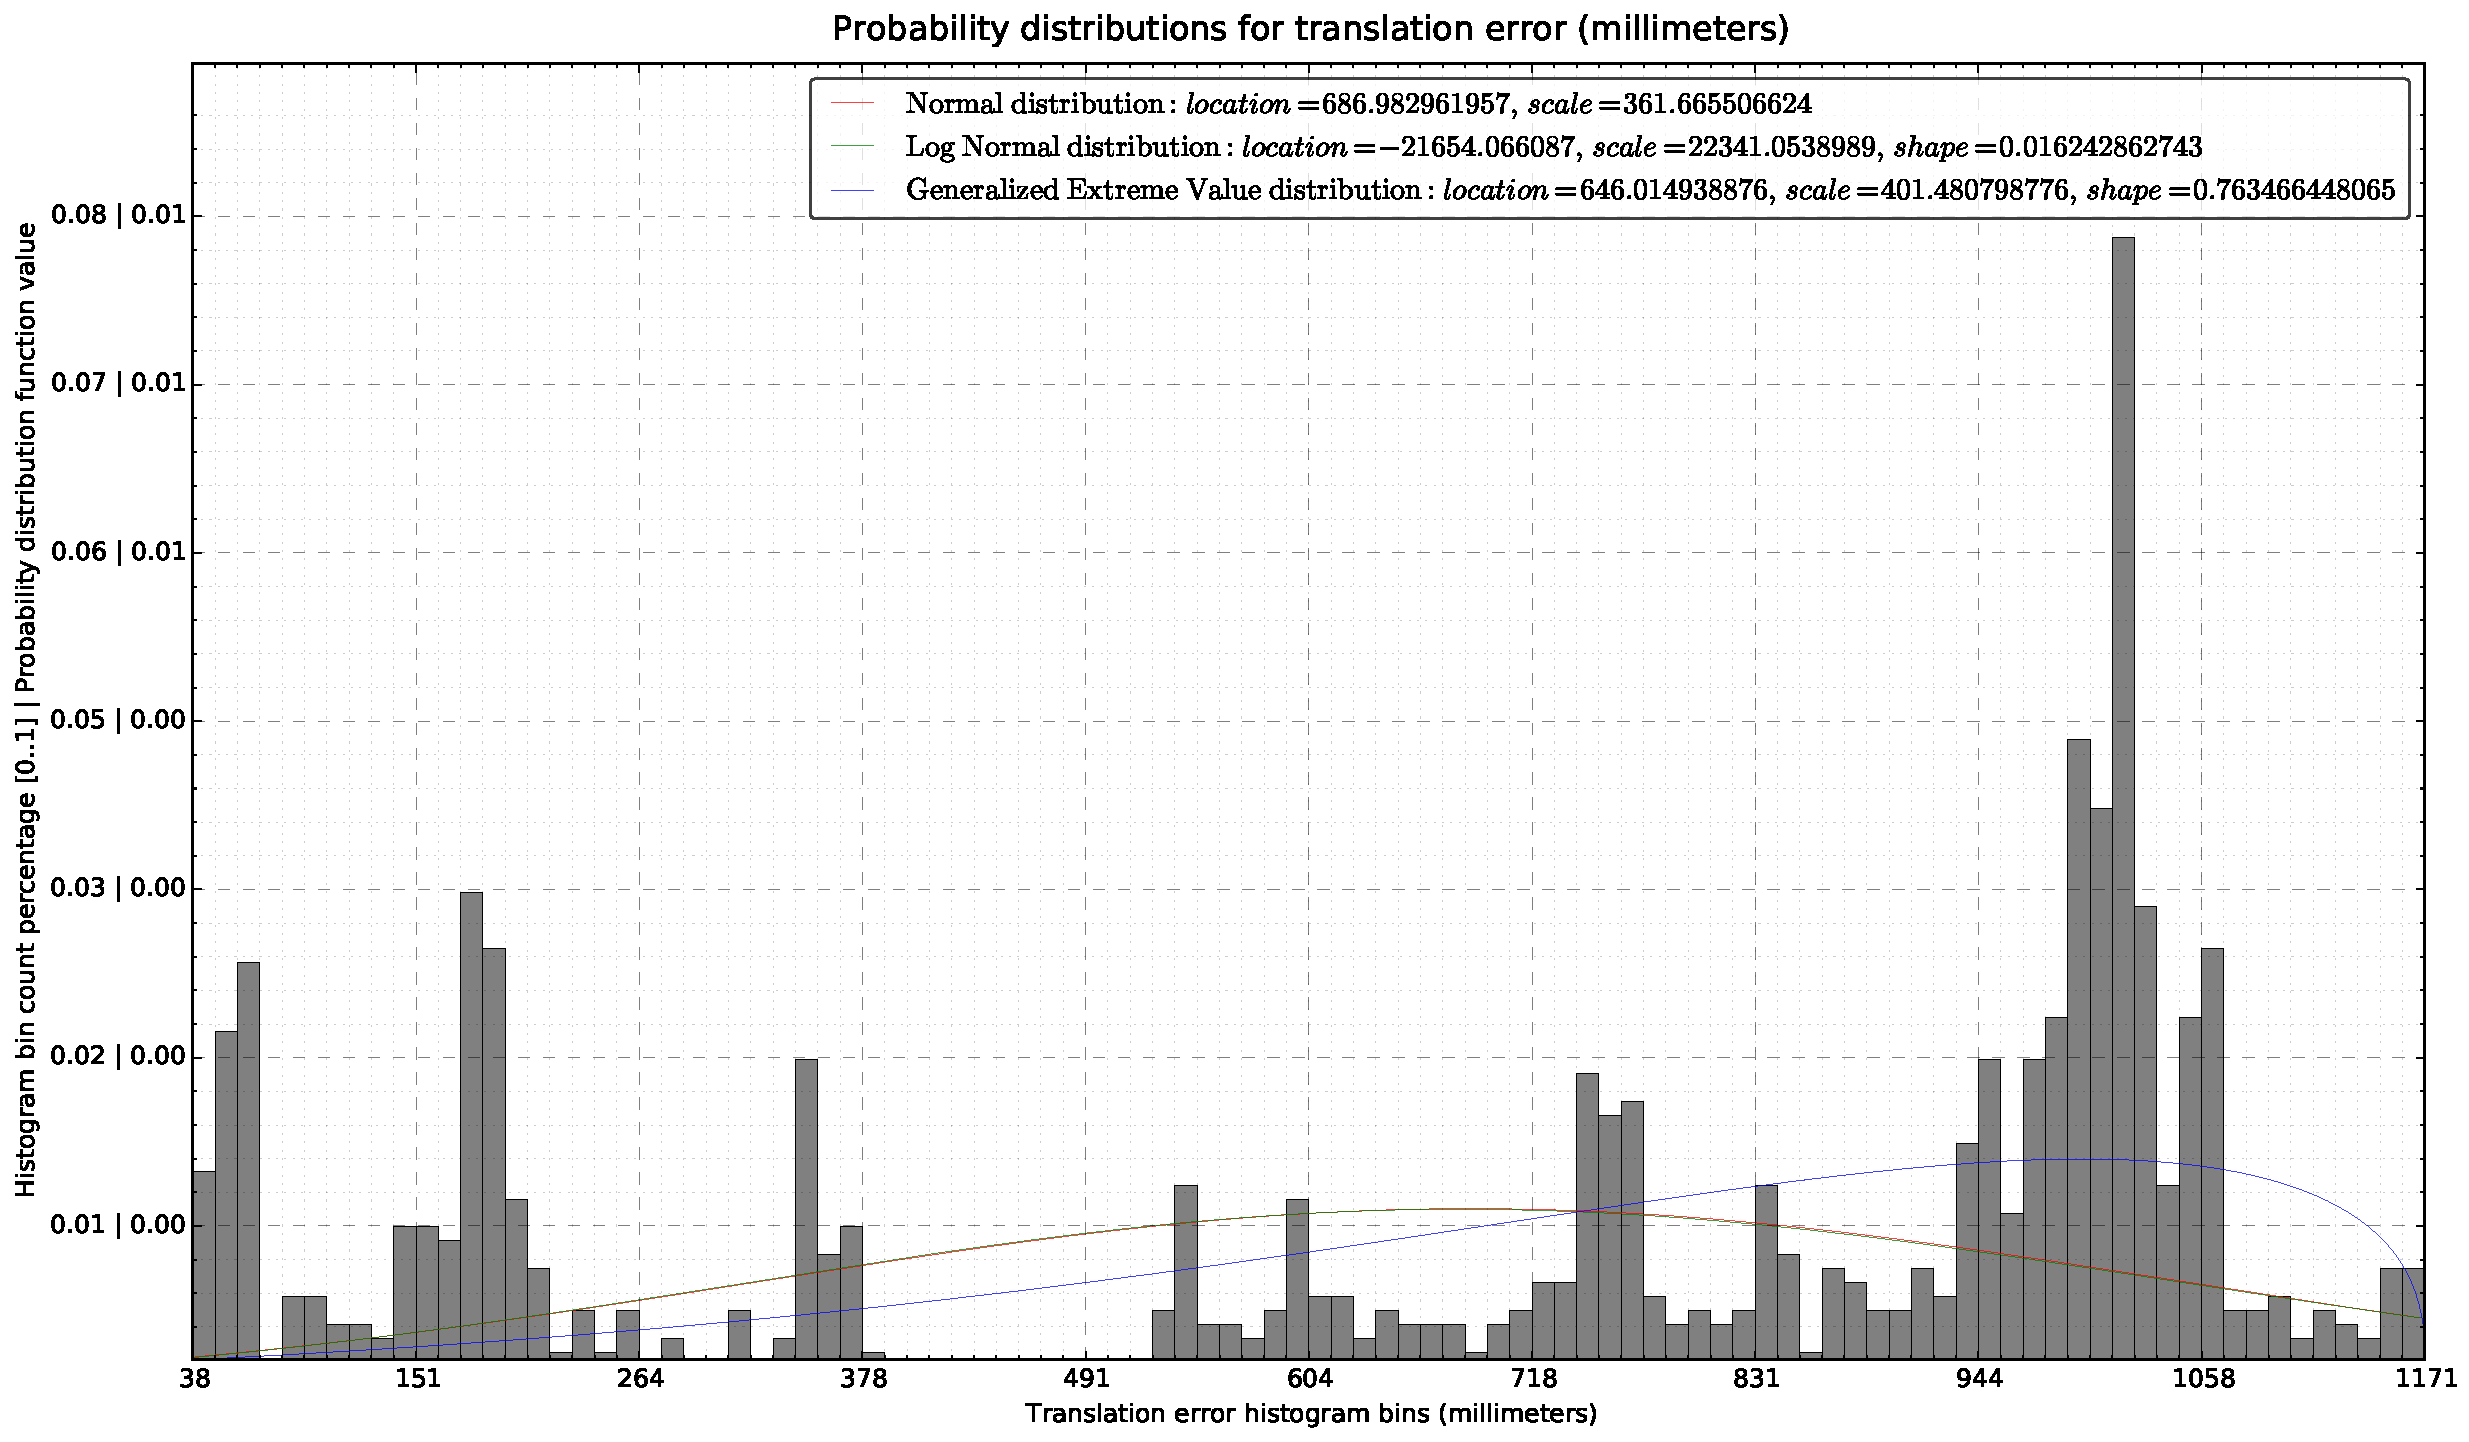
\includegraphics[width=0.73\textwidth]{appendices/tests-3dof/pioneer-robot/\currfilebase/graphs/odometry-translation-error-millimeters-distributions}
	\caption{Probability distributions for the odometry translation errors}
\end{figure}

\begin{figure}[H]
	\centering
	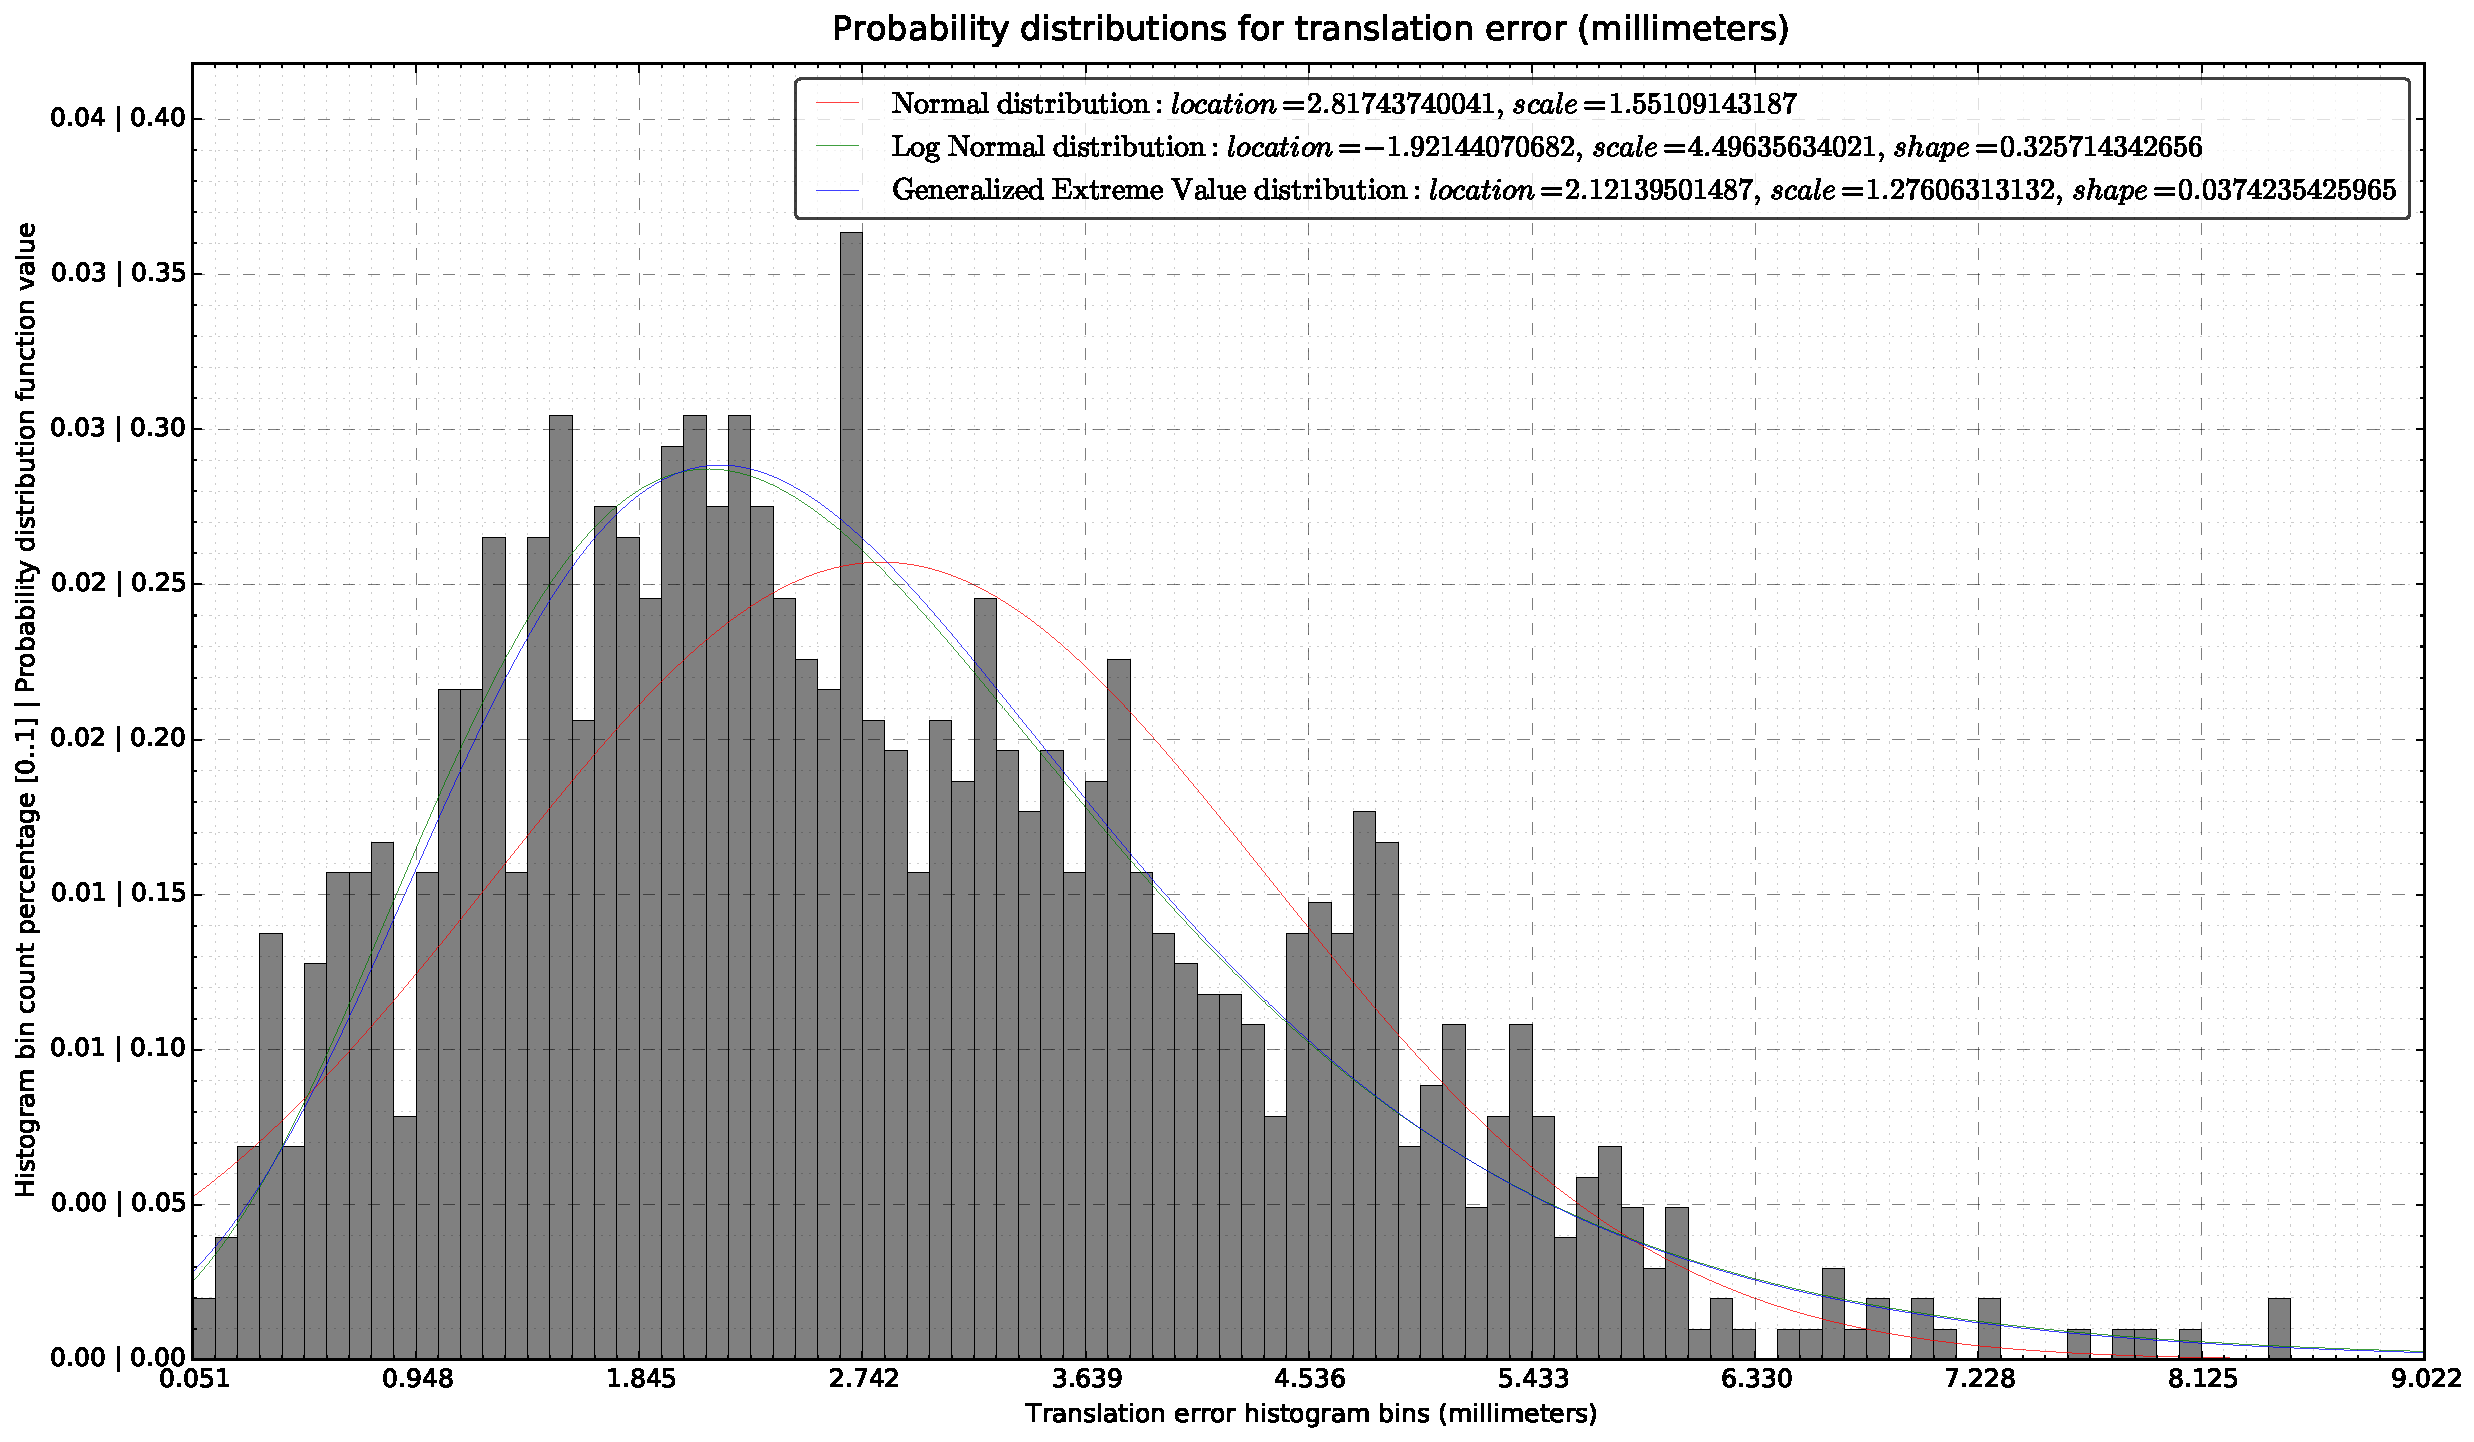
\includegraphics[width=0.73\textwidth]{appendices/tests-3dof/pioneer-robot/\currfilebase/graphs/translation-error-millimeters-distributions}
	\caption{Probability distributions for the localization system translation errors}
\end{figure}

\begin{figure}[H]
	\centering
	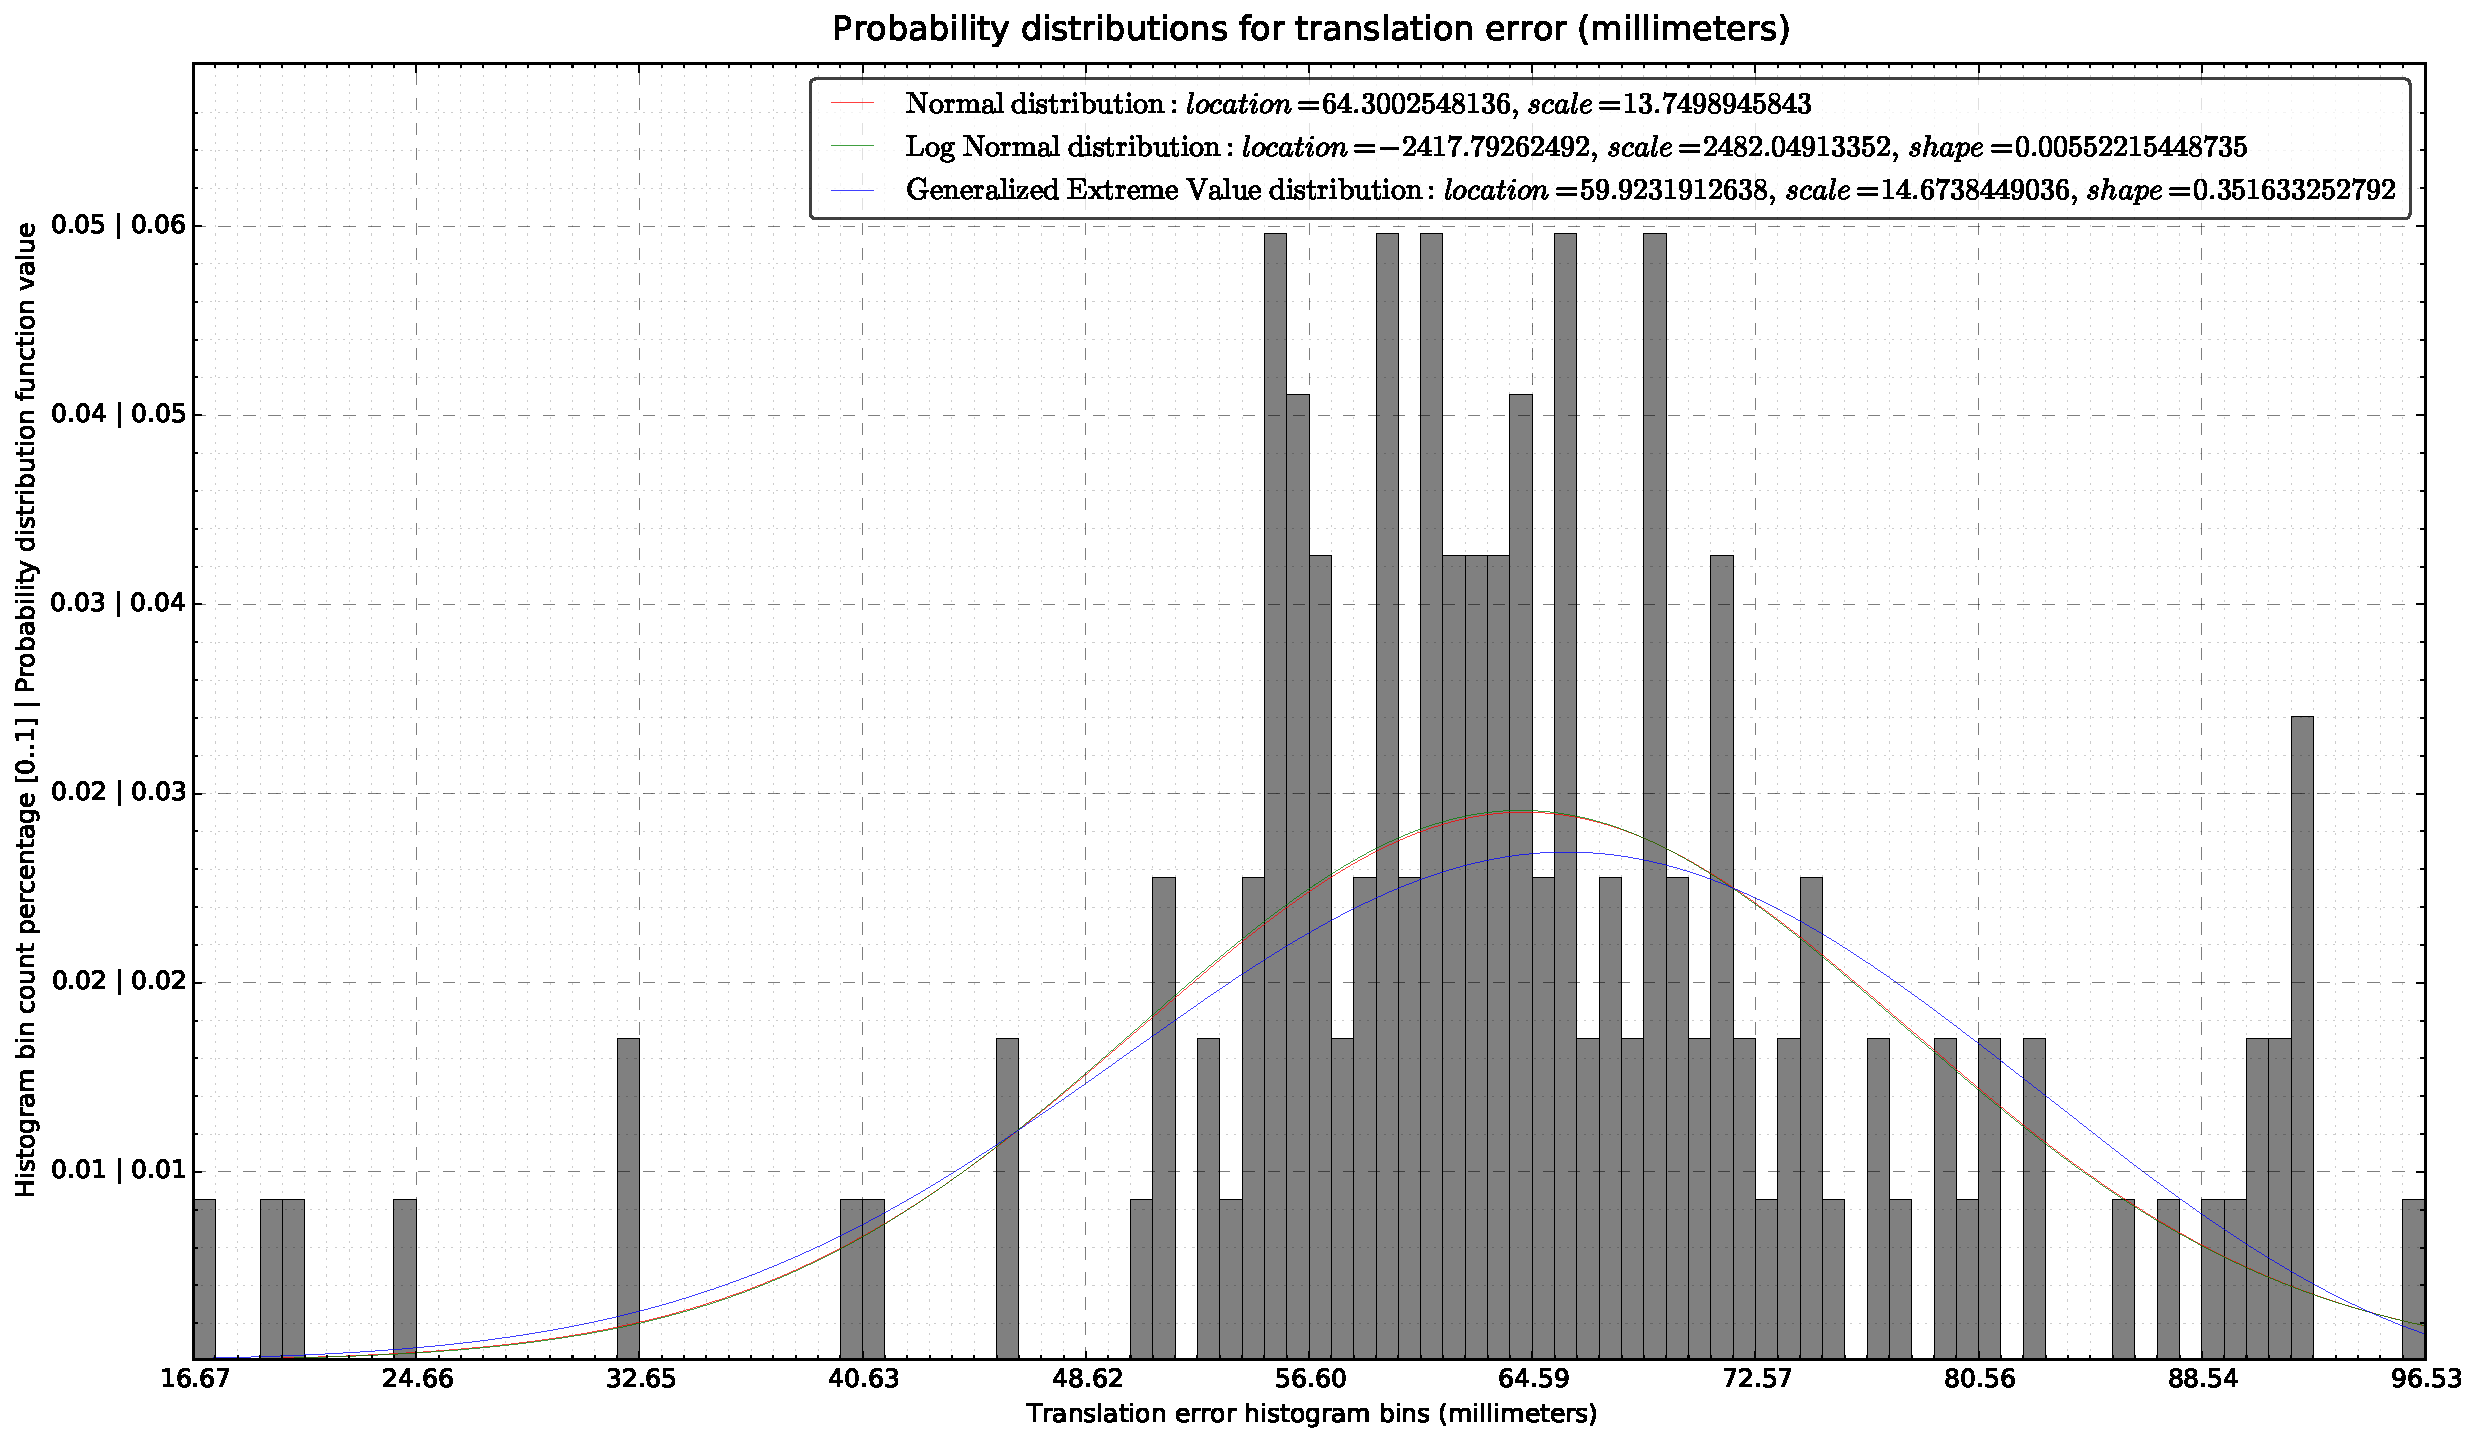
\includegraphics[width=0.73\textwidth]{appendices/tests-3dof/pioneer-robot/\currfilebase/graphs/translation-error-millimeters-distributions-amcl}
	\caption{Probability distributions for the \glsentrytext{amcl} translation errors}
\end{figure}


%Angular errors axis
\begin{figure}[H]
	\centering
	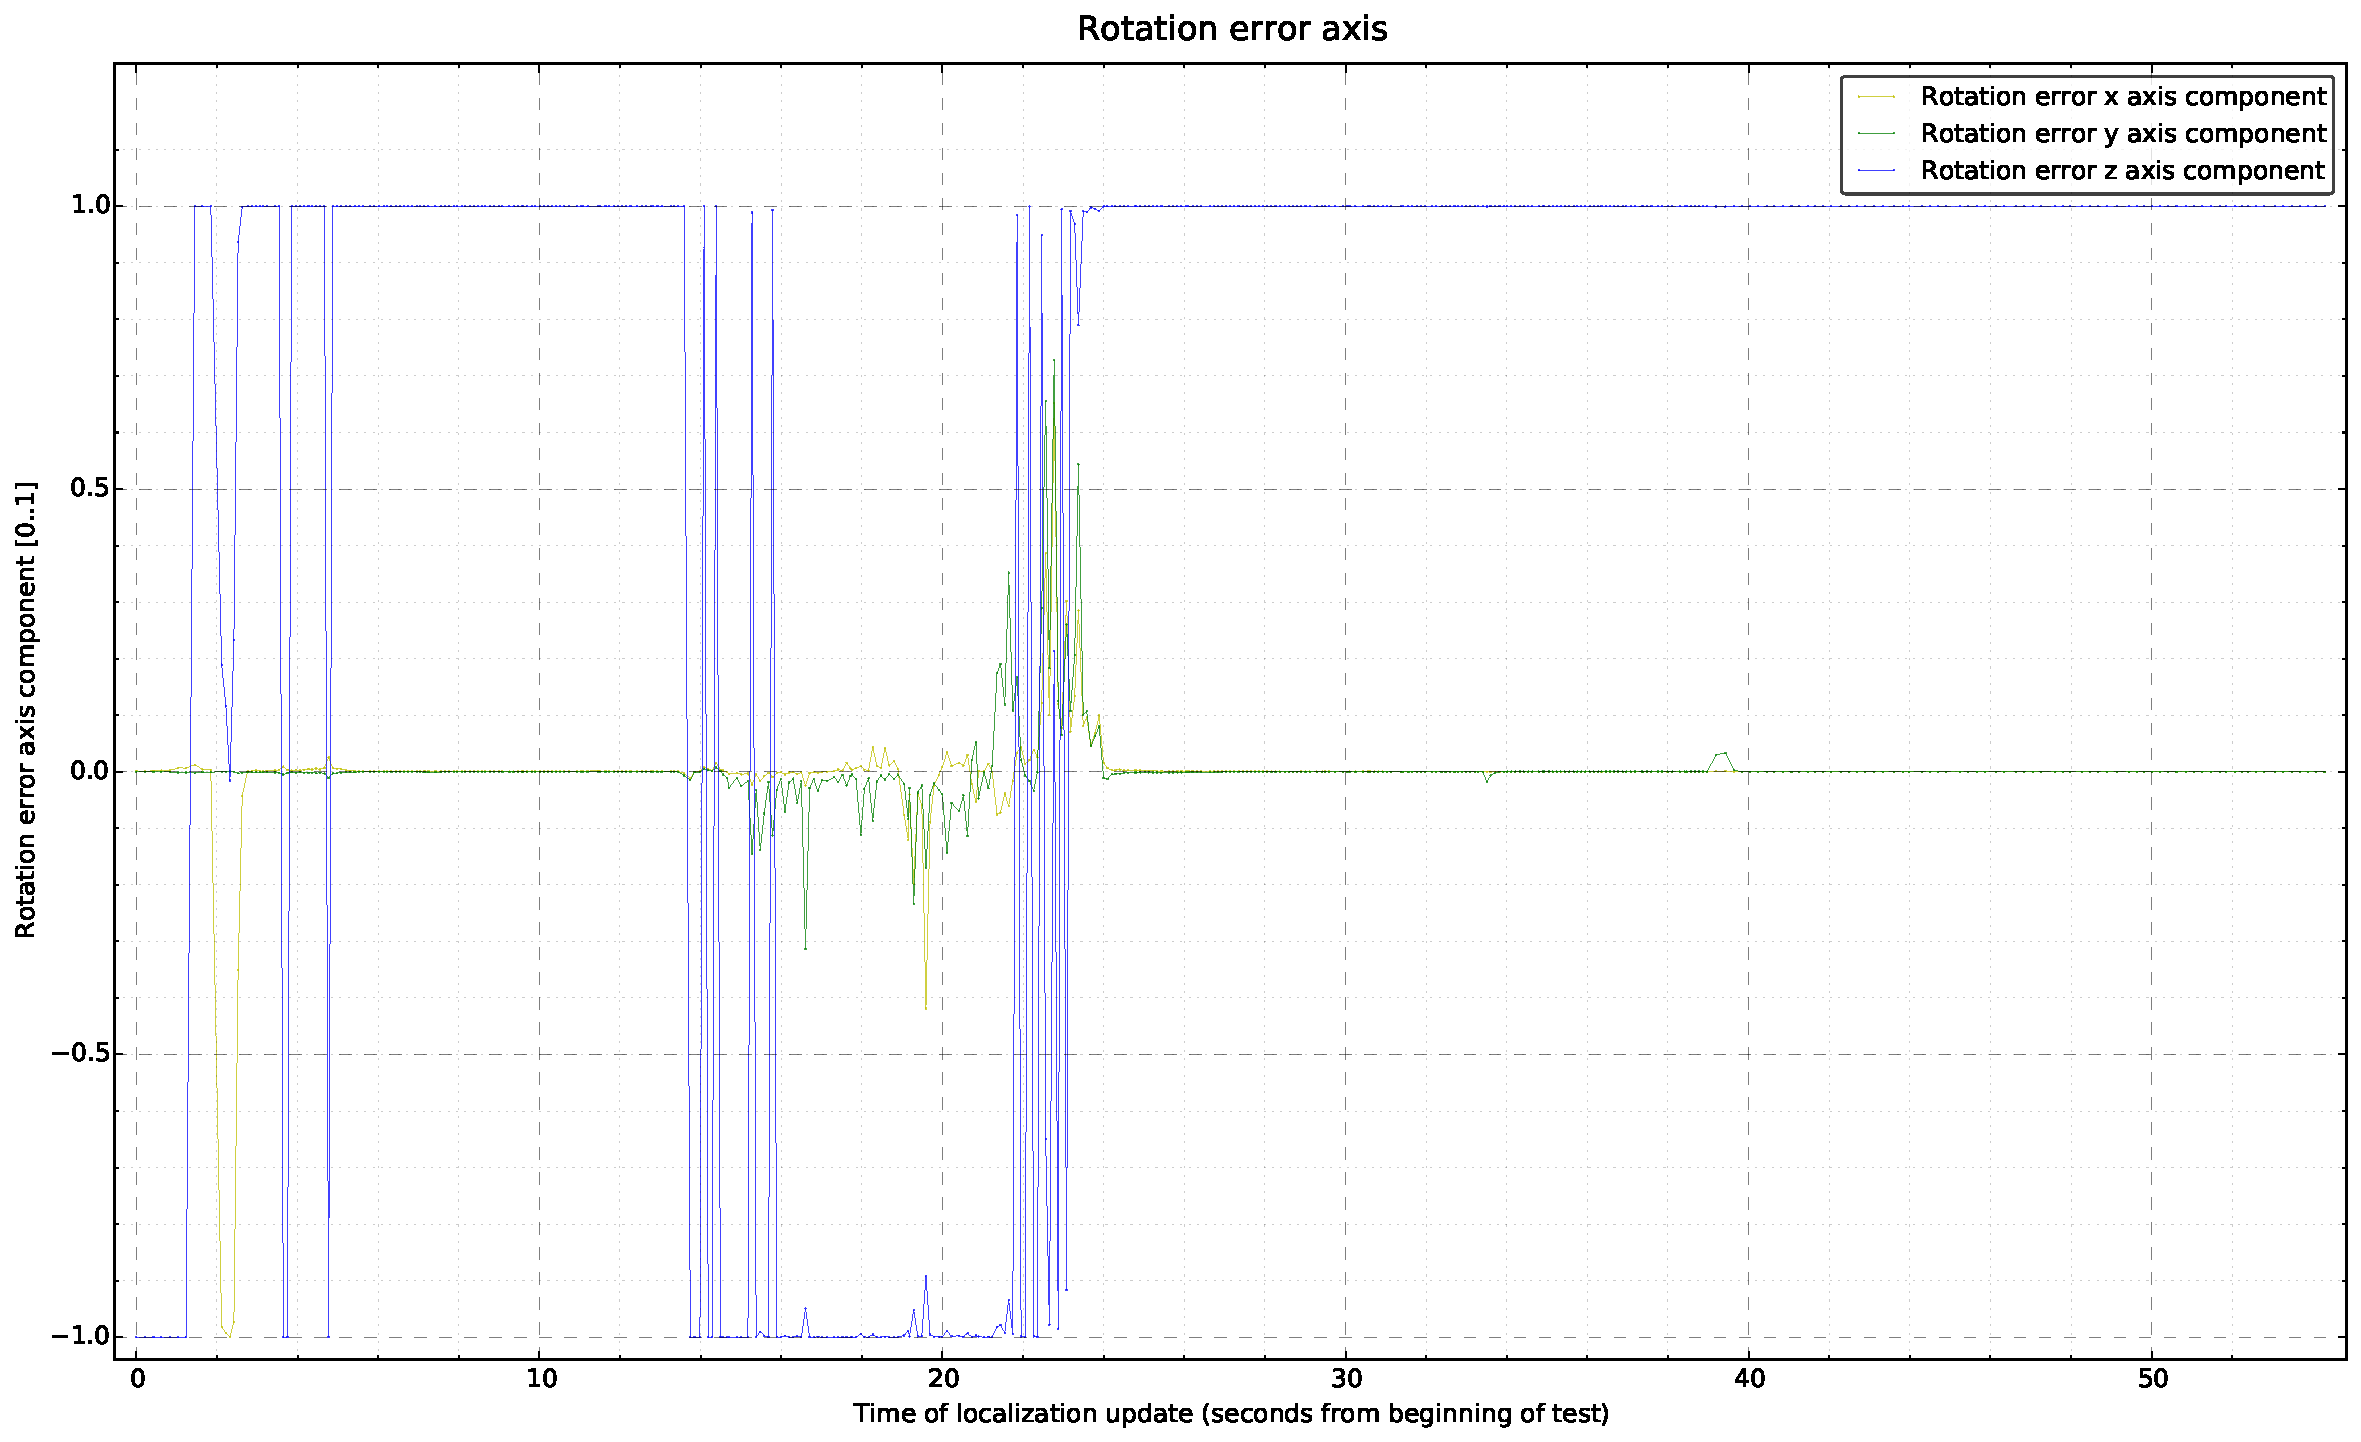
\includegraphics[width=0.69\textwidth]{appendices/tests-3dof/pioneer-robot/\currfilebase/graphs/odometry-rotation-error-axis}
	\caption{Odometry rotation errors axis}
\end{figure}

\begin{figure}[H]
	\centering
	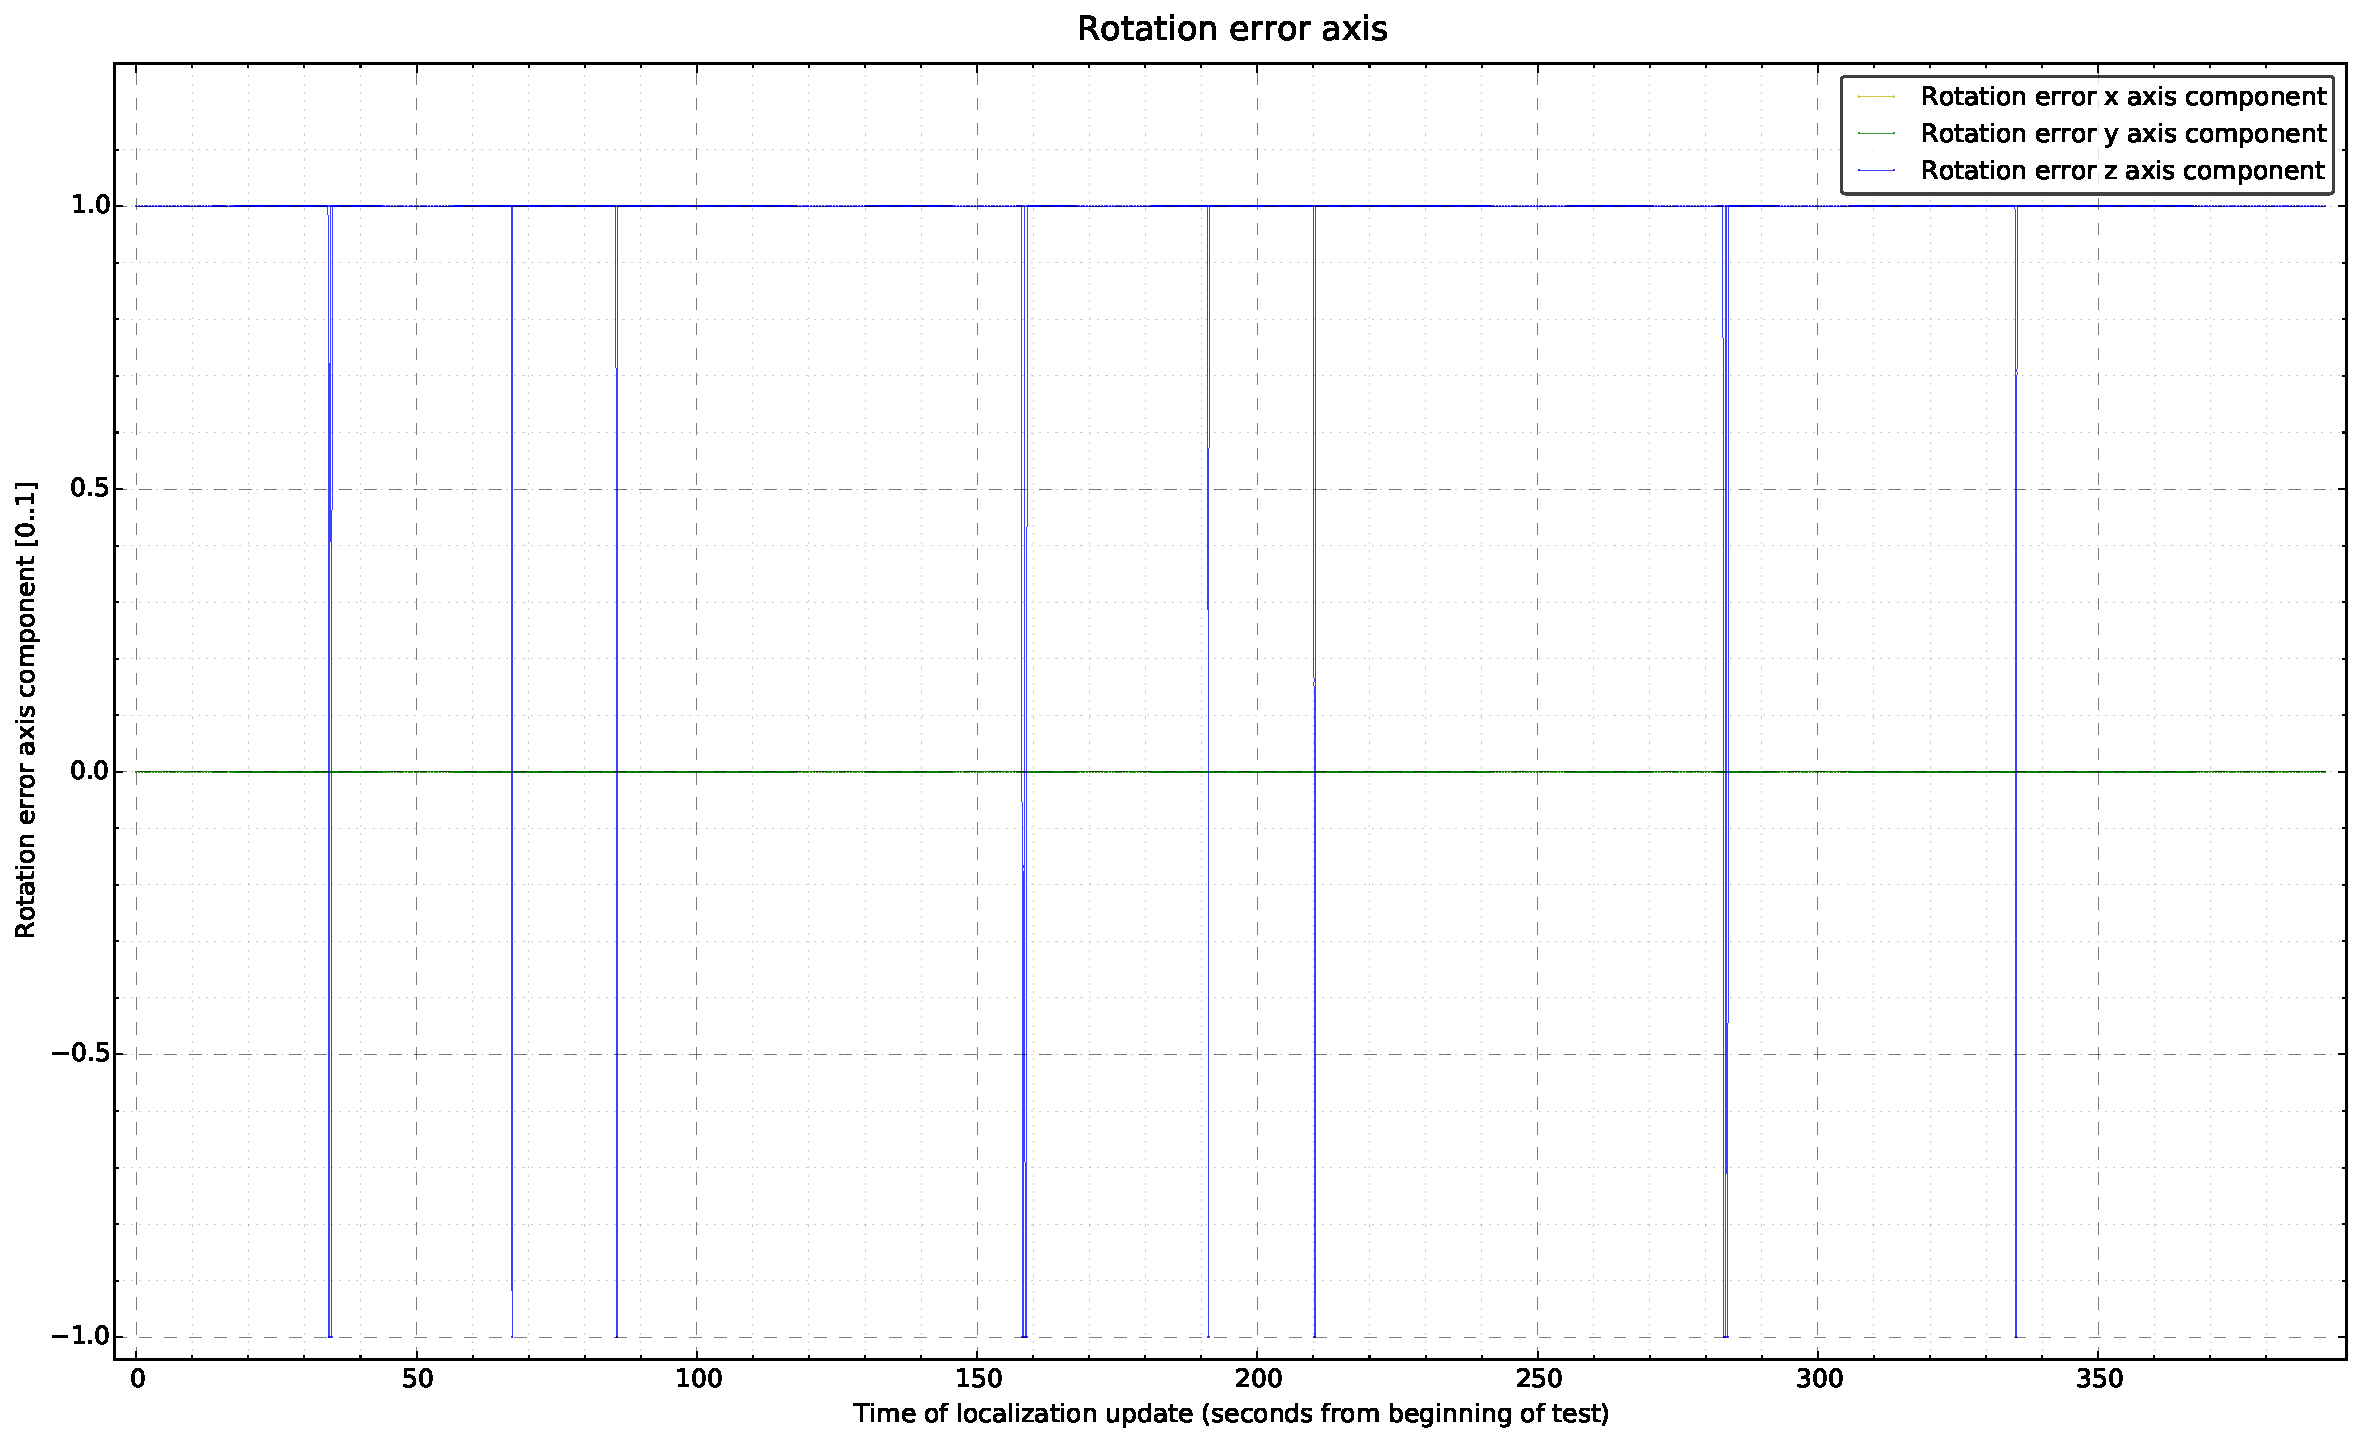
\includegraphics[width=0.69\textwidth]{appendices/tests-3dof/pioneer-robot/\currfilebase/graphs/rotation-error-axis}
	\caption{Localization system rotation errors axis}
\end{figure}

\begin{figure}[H]
	\centering
	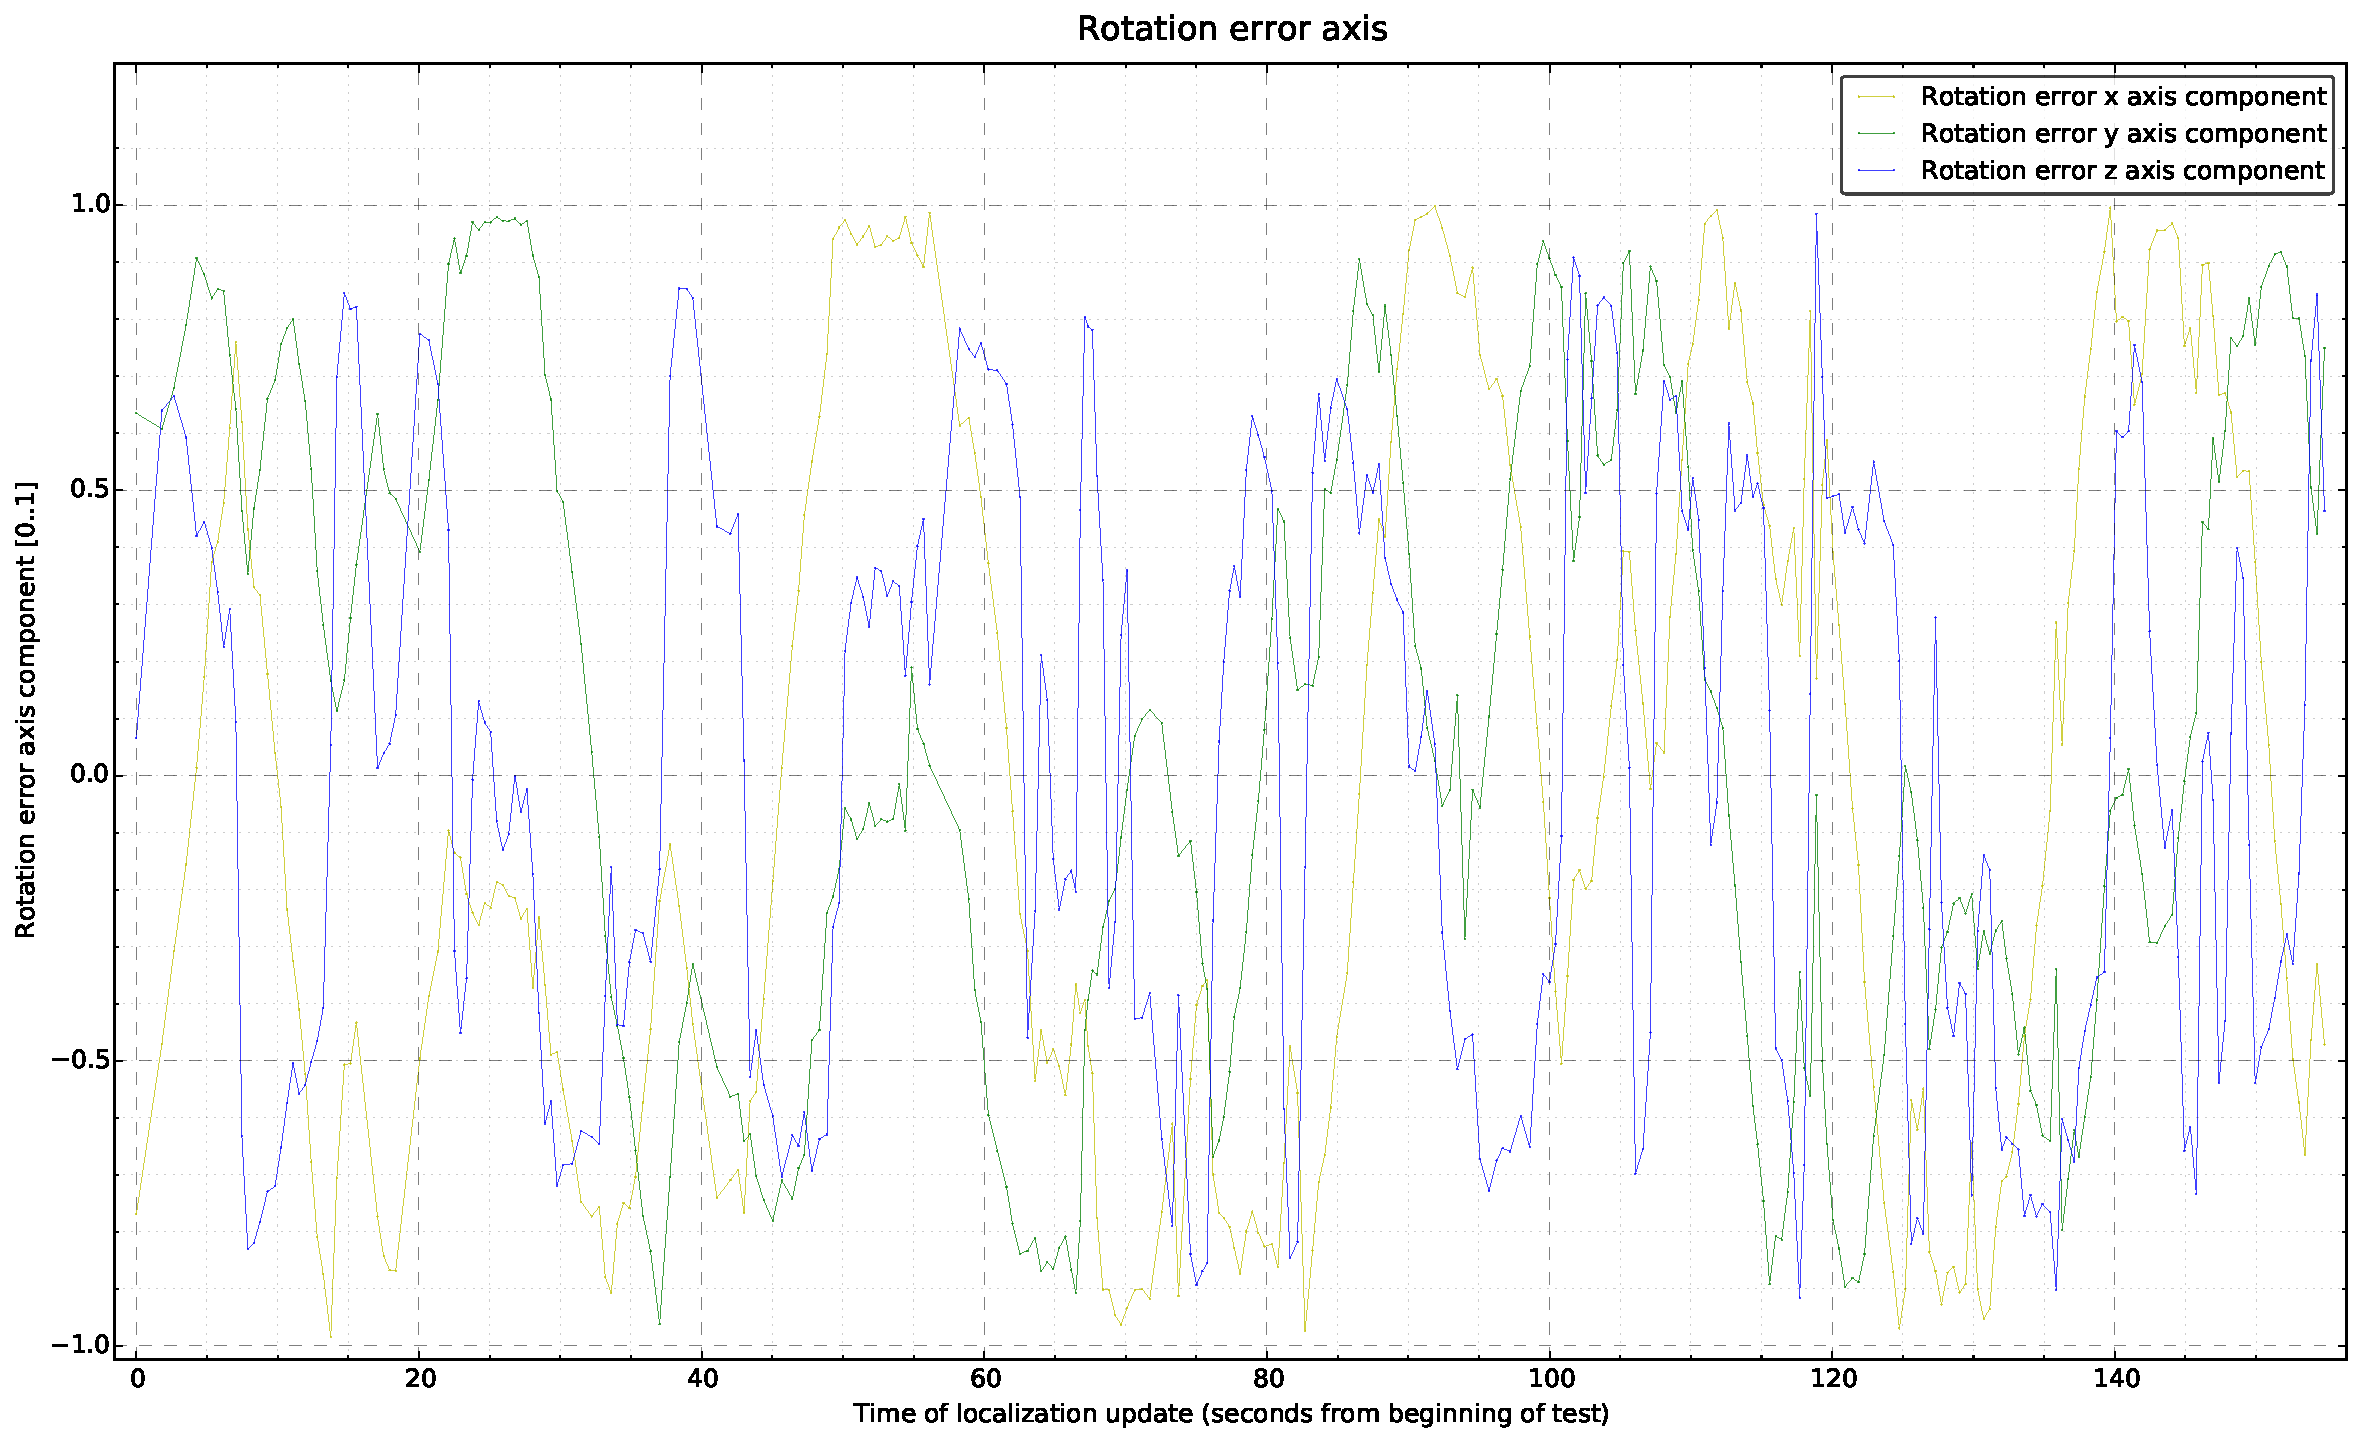
\includegraphics[width=0.69\textwidth]{appendices/tests-3dof/pioneer-robot/\currfilebase/graphs/rotation-error-axis-amcl}
	\caption{\glsentrytext{amcl} rotation errors axis}
\end{figure}


%Angular errors
\begin{figure}[H]
	\centering
	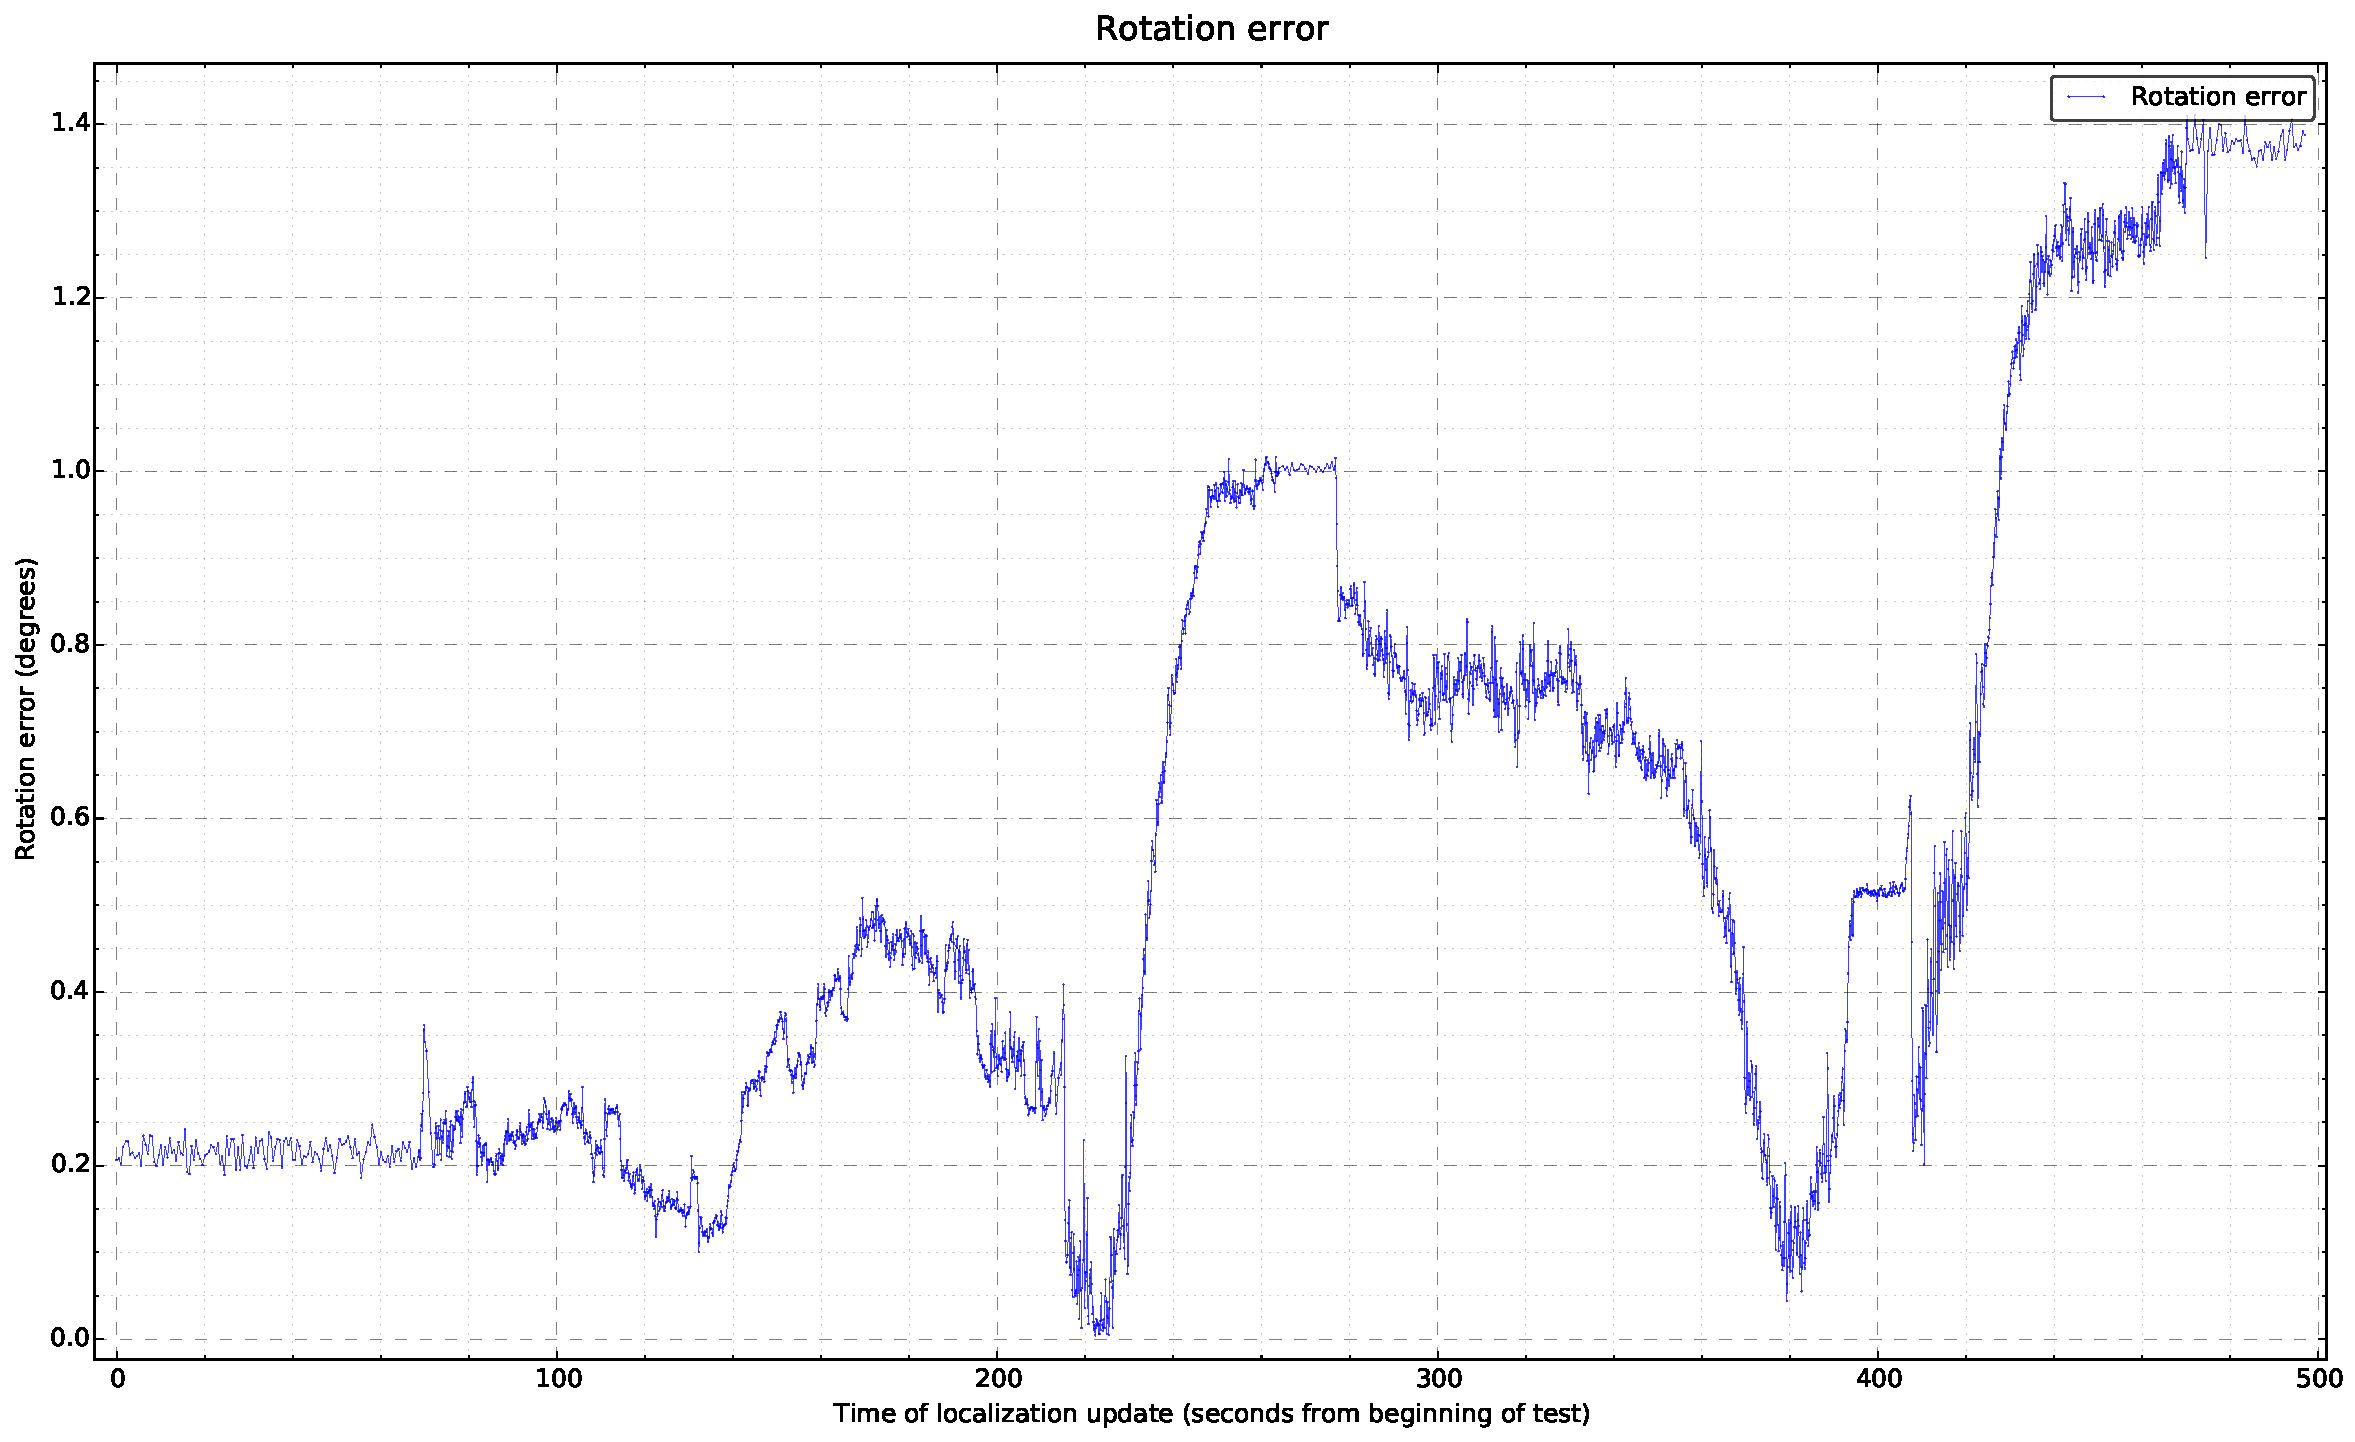
\includegraphics[width=0.69\textwidth]{appendices/tests-3dof/pioneer-robot/\currfilebase/graphs/odometry-rotation-error-degrees}
	\caption{Odometry rotation errors}
\end{figure}

\begin{figure}[H]
	\centering
	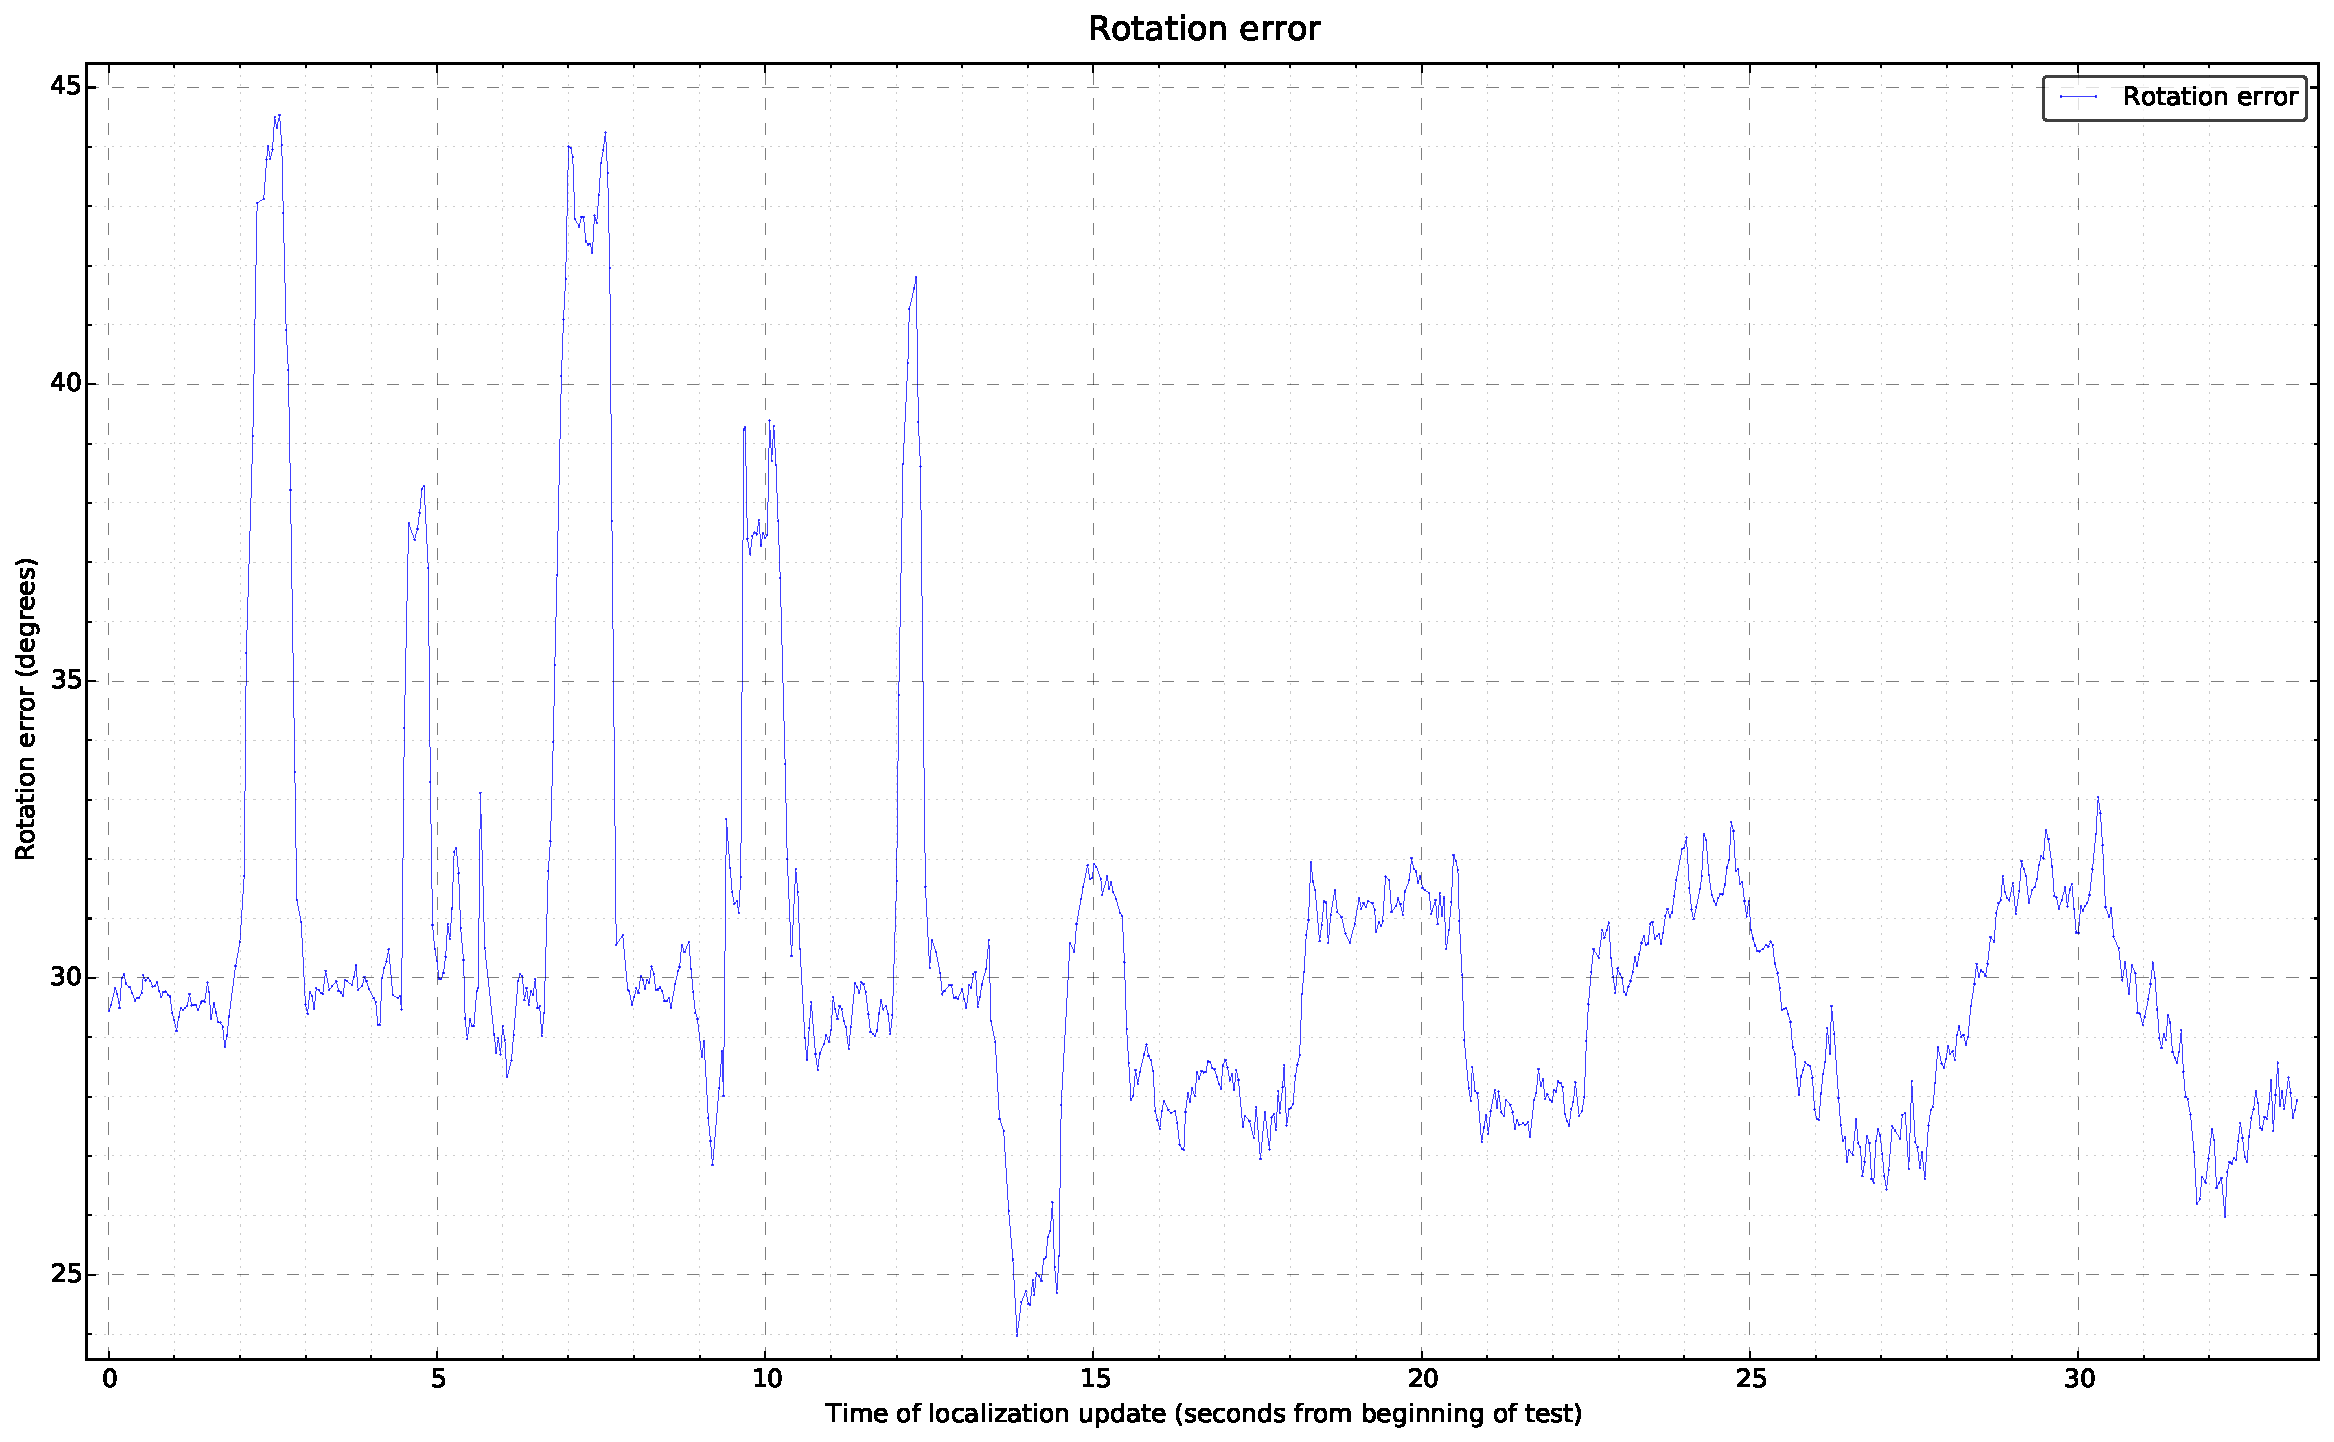
\includegraphics[width=0.69\textwidth]{appendices/tests-3dof/pioneer-robot/\currfilebase/graphs/rotation-error-degrees}
	\caption{Localization system rotation errors}
\end{figure}

\begin{figure}[H]
	\centering
	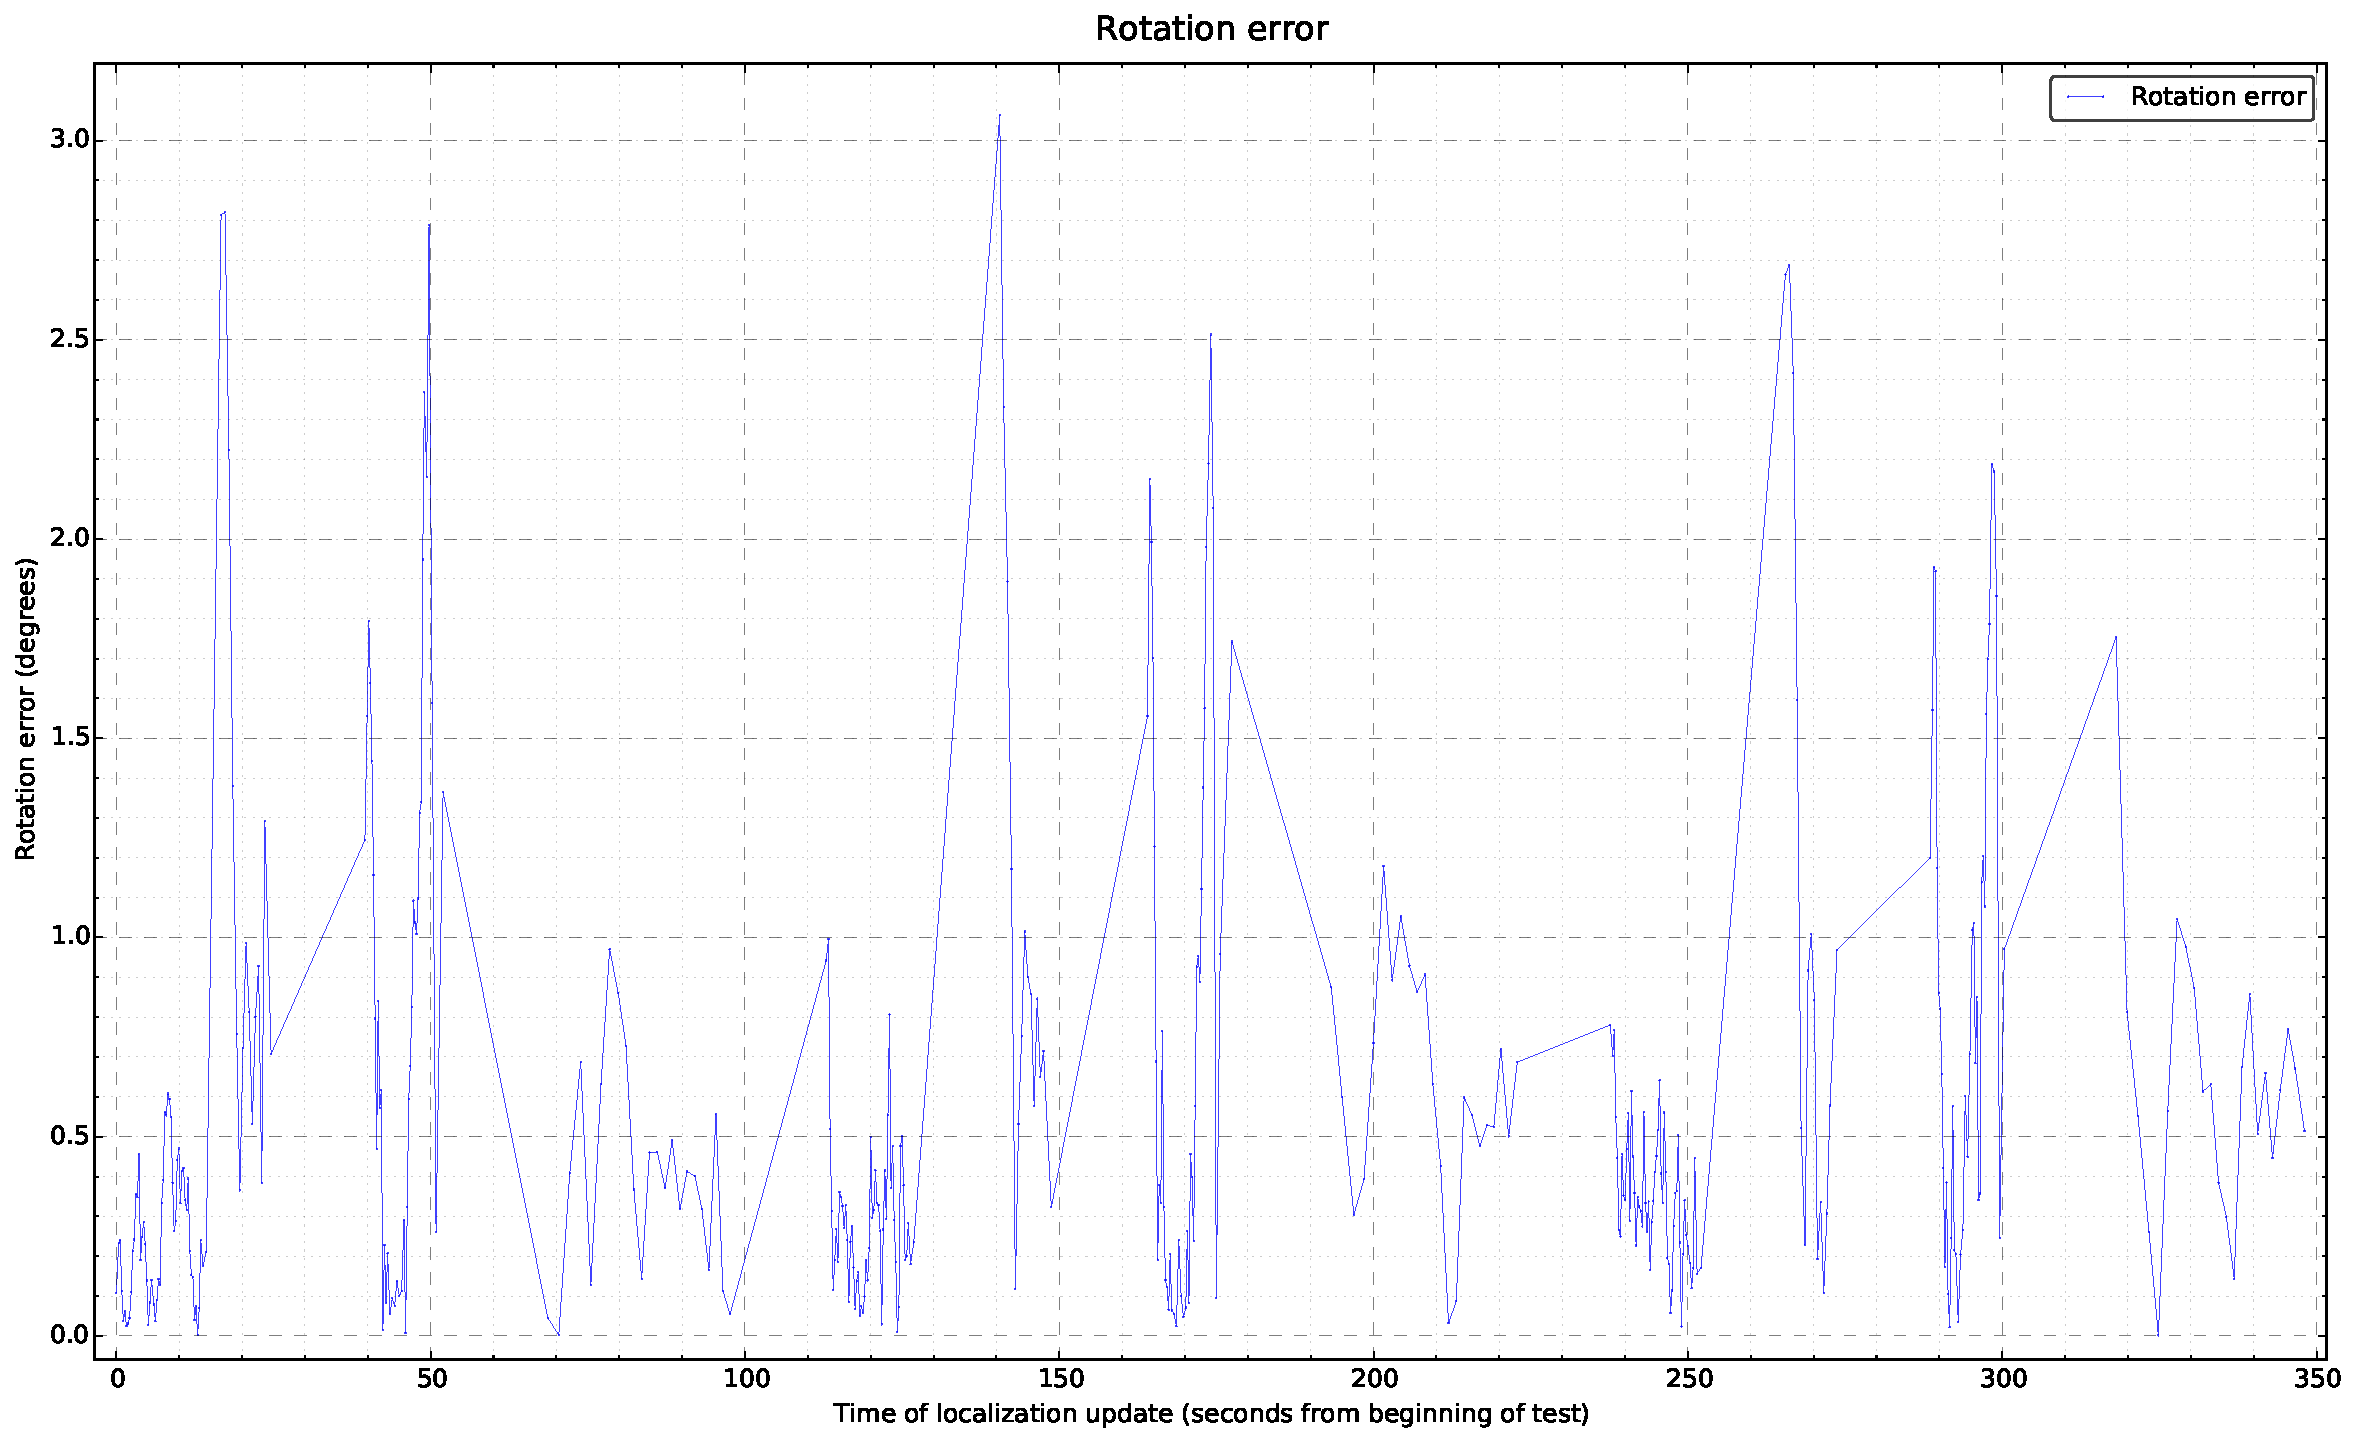
\includegraphics[width=0.69\textwidth]{appendices/tests-3dof/pioneer-robot/\currfilebase/graphs/rotation-error-degrees-amcl}
	\caption{\glsentrytext{amcl} rotation errors}
\end{figure}


%Angular errors distributions
\begin{figure}[H]
	\centering
	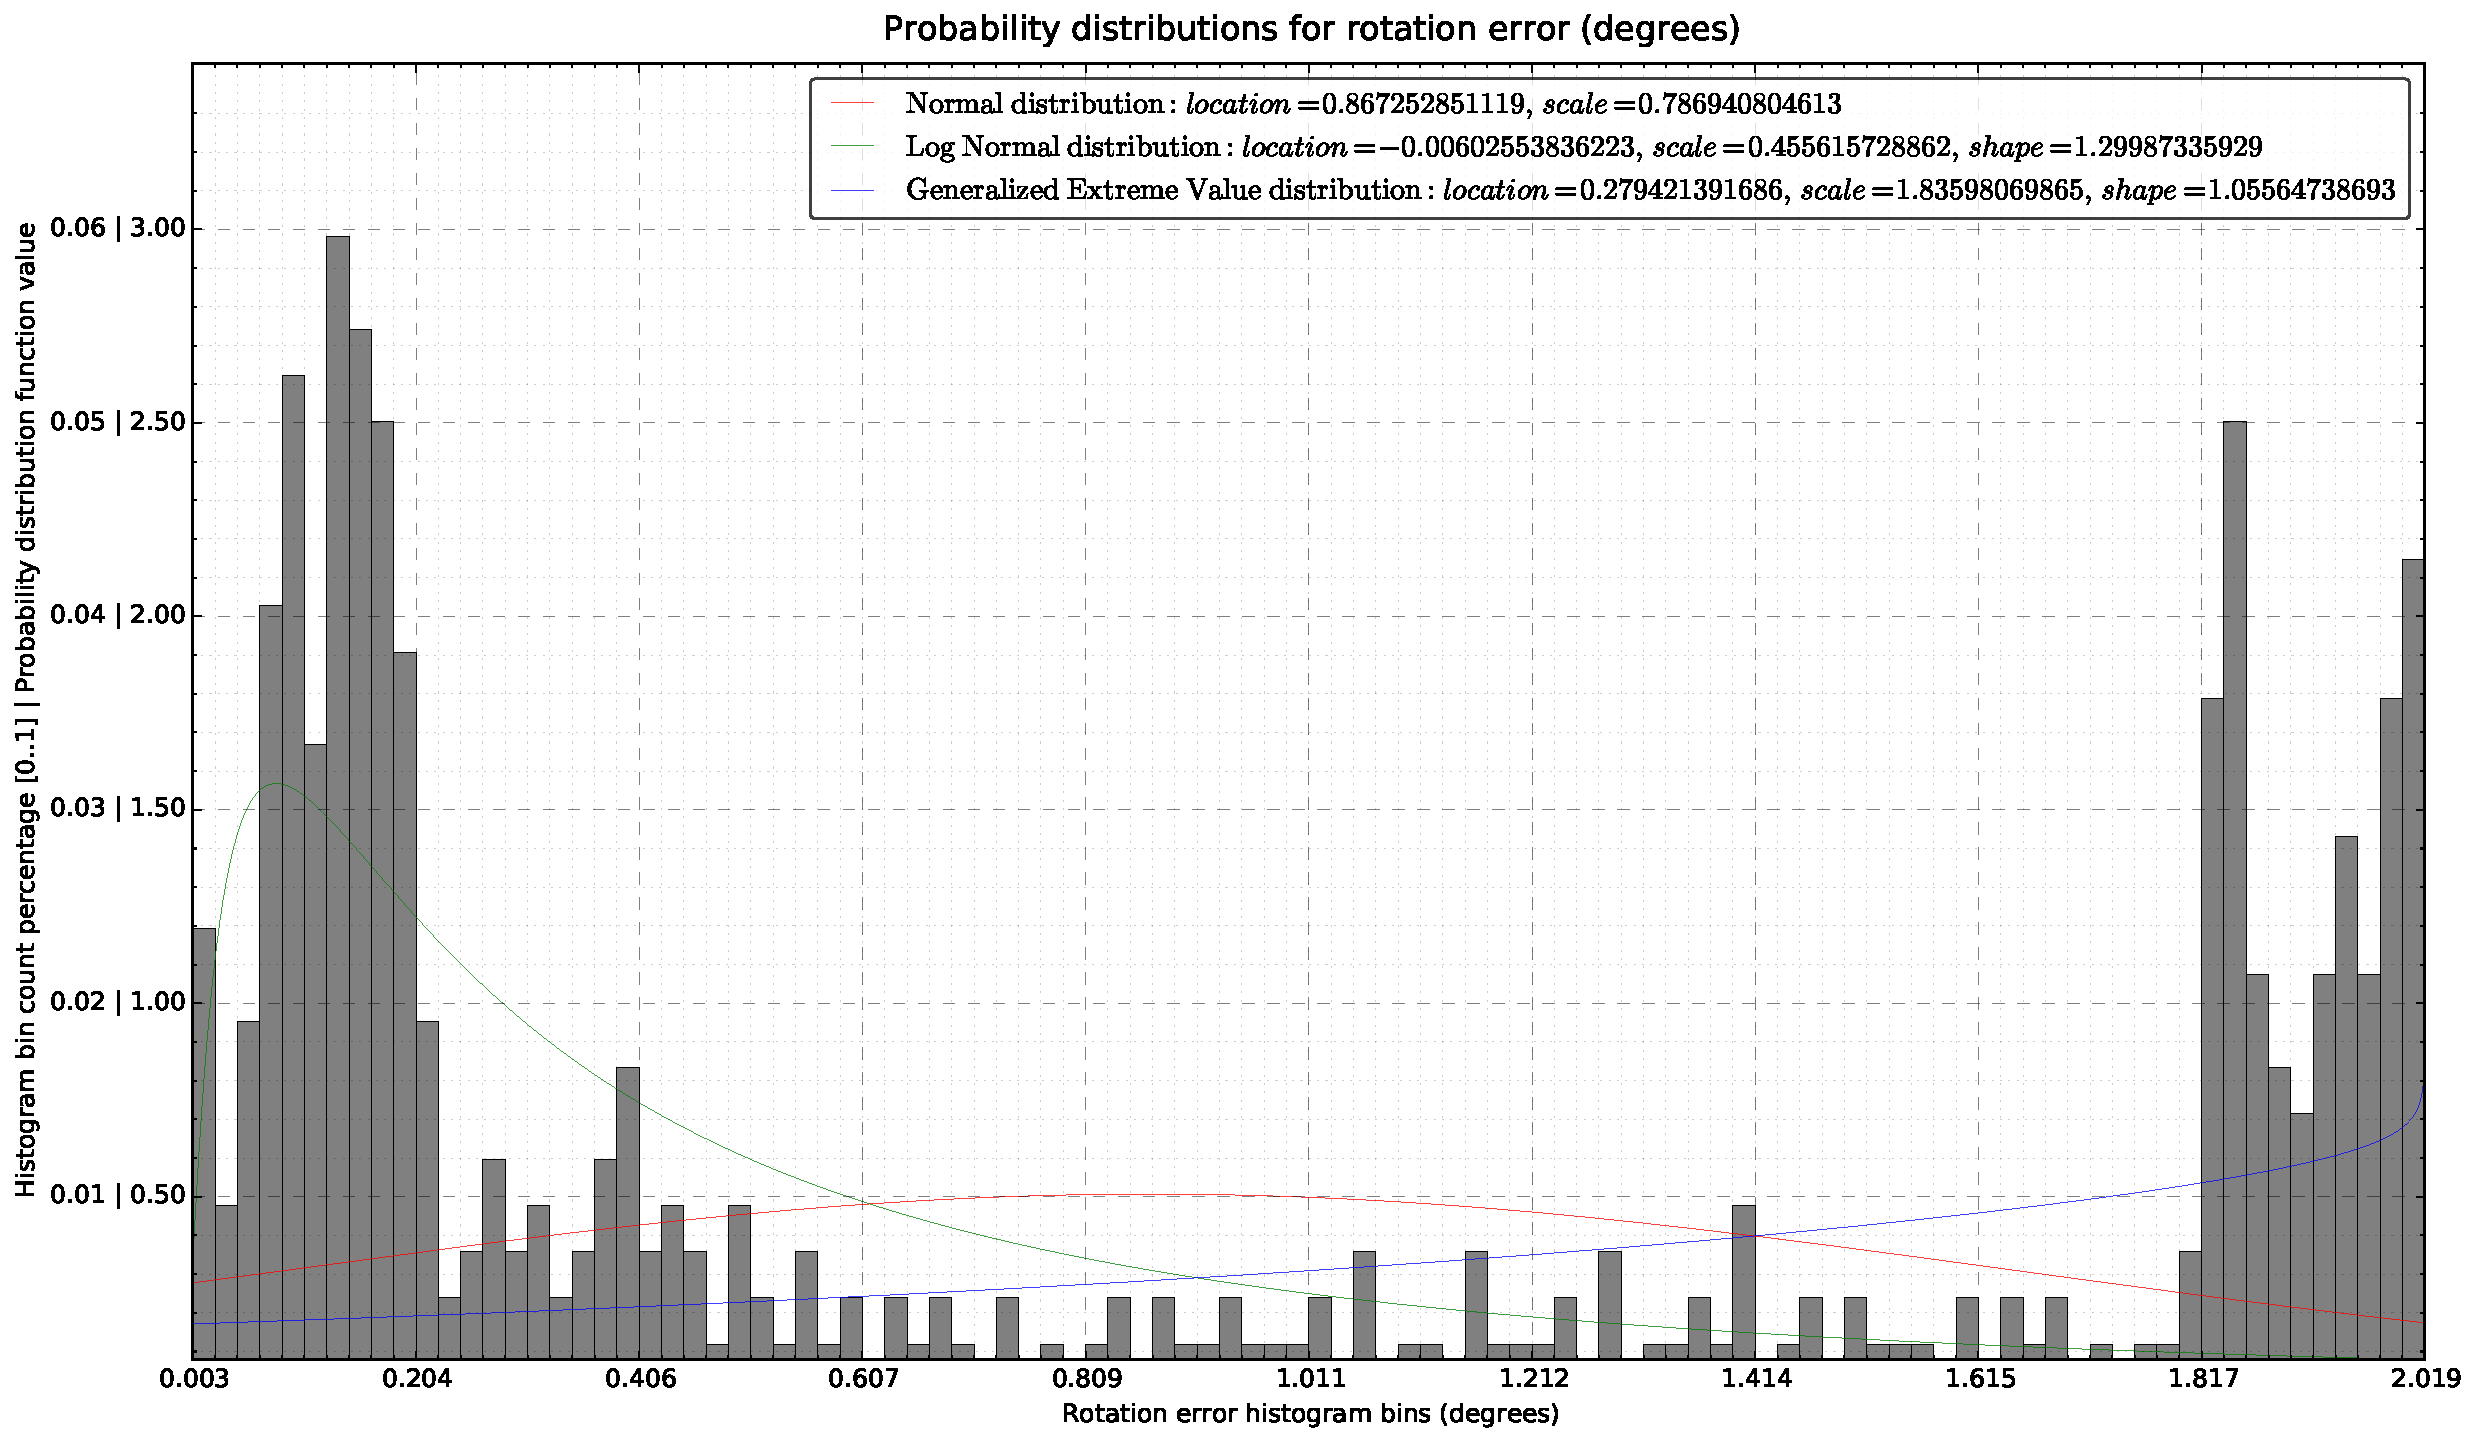
\includegraphics[width=0.73\textwidth]{appendices/tests-3dof/pioneer-robot/\currfilebase/graphs/odometry-rotation-error-degrees-distributions}
	\caption{Probability distributions for the odometry rotation errors}
\end{figure}

\begin{figure}[H]
	\centering
	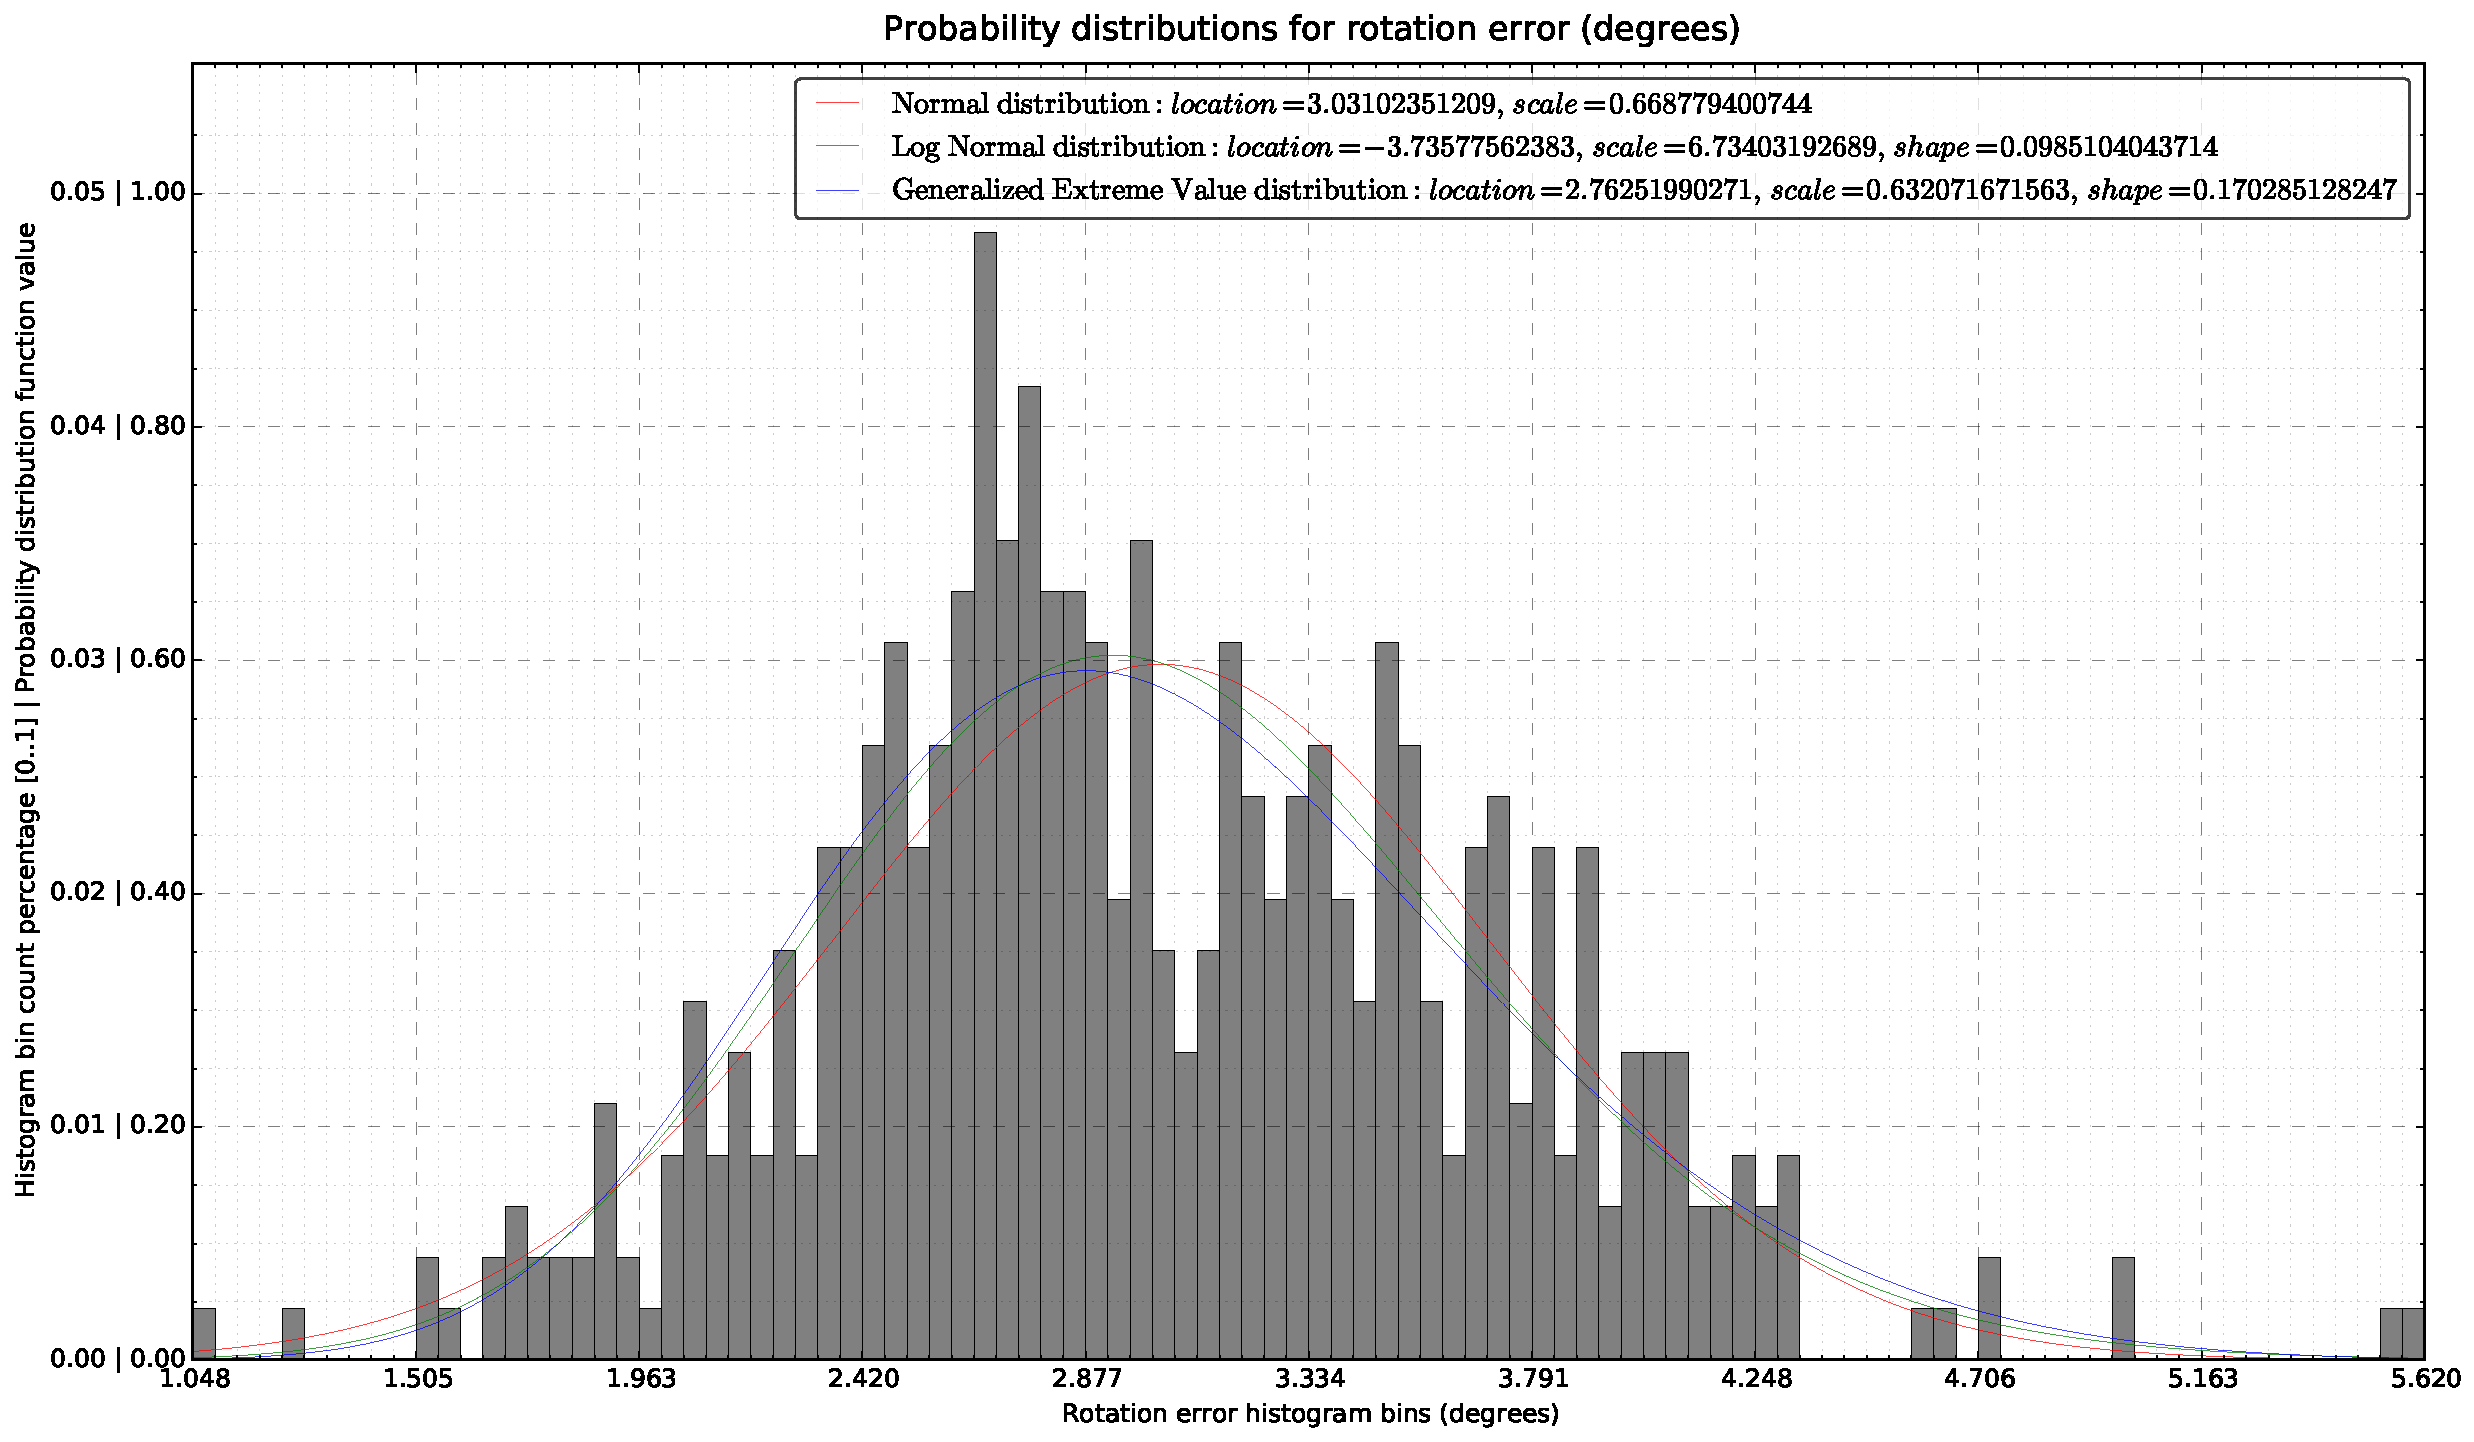
\includegraphics[width=0.73\textwidth]{appendices/tests-3dof/pioneer-robot/\currfilebase/graphs/rotation-error-degrees-distributions}
	\caption{Probability distributions for the localization system rotation errors}
\end{figure}

\begin{figure}[H]
	\centering
	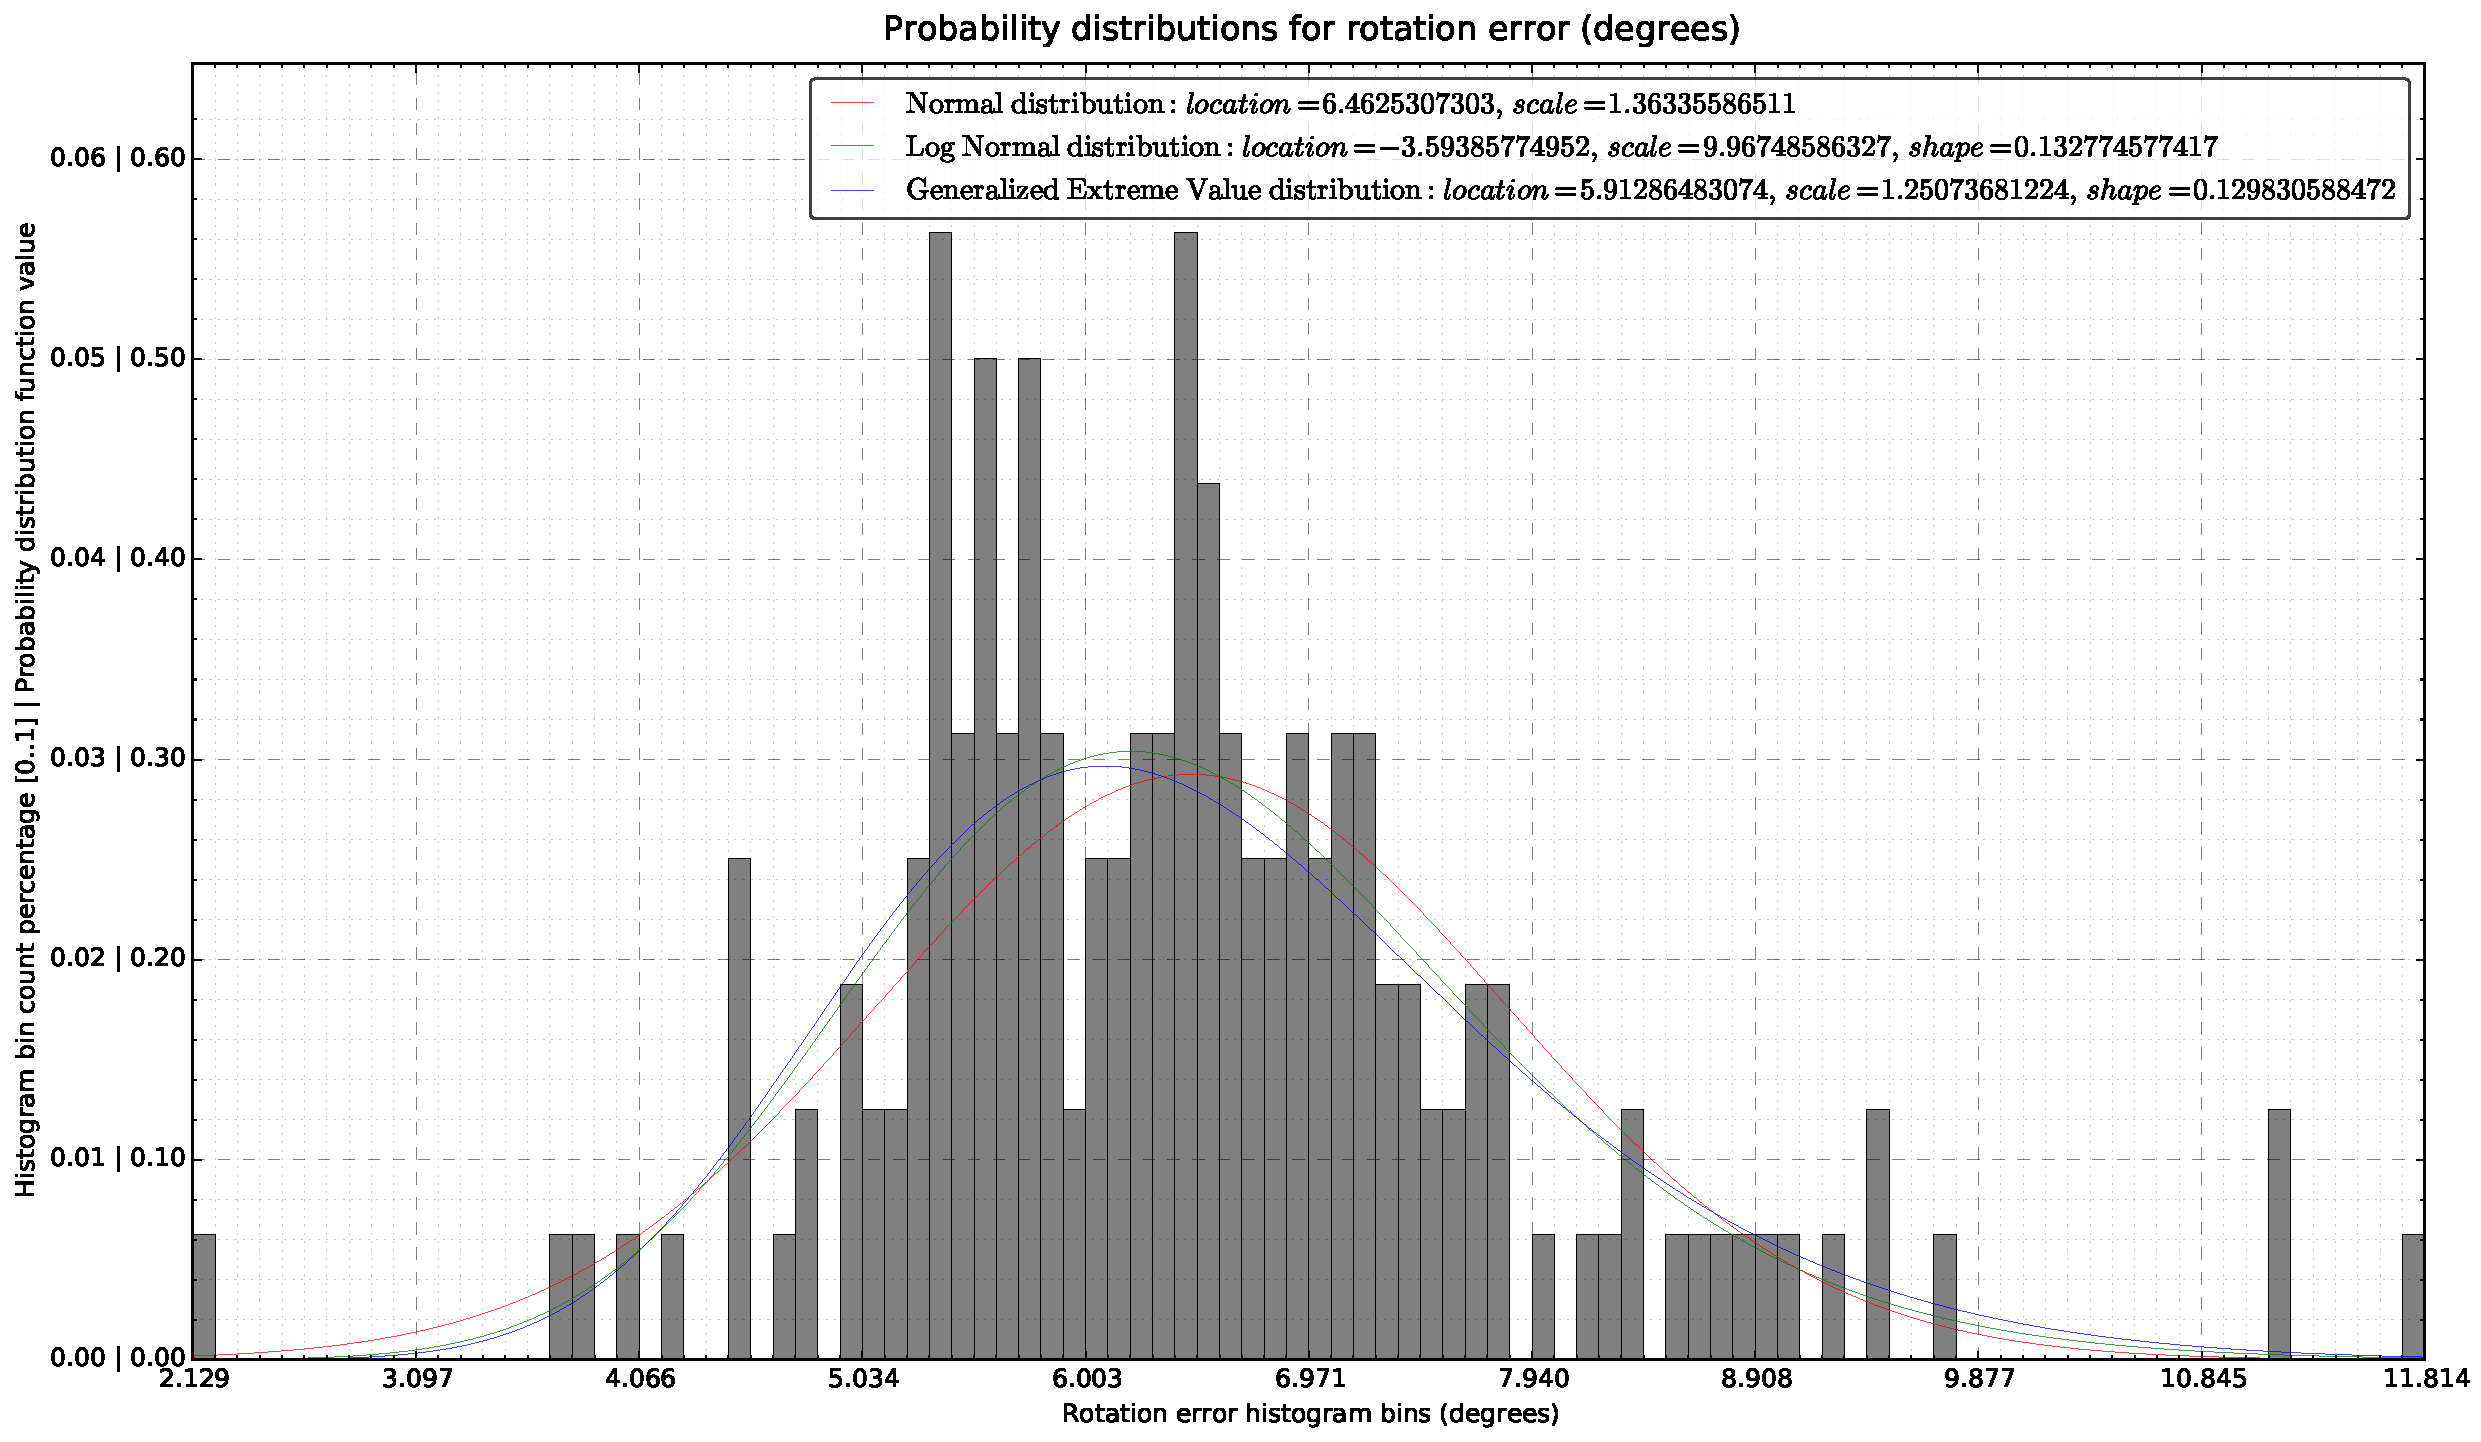
\includegraphics[width=0.73\textwidth]{appendices/tests-3dof/pioneer-robot/\currfilebase/graphs/rotation-error-degrees-distributions-amcl}
	\caption{Probability distributions for the \glsentrytext{amcl} rotation errors}
\end{figure}


%Translation corrections
\begin{figure}[H]
	\centering
	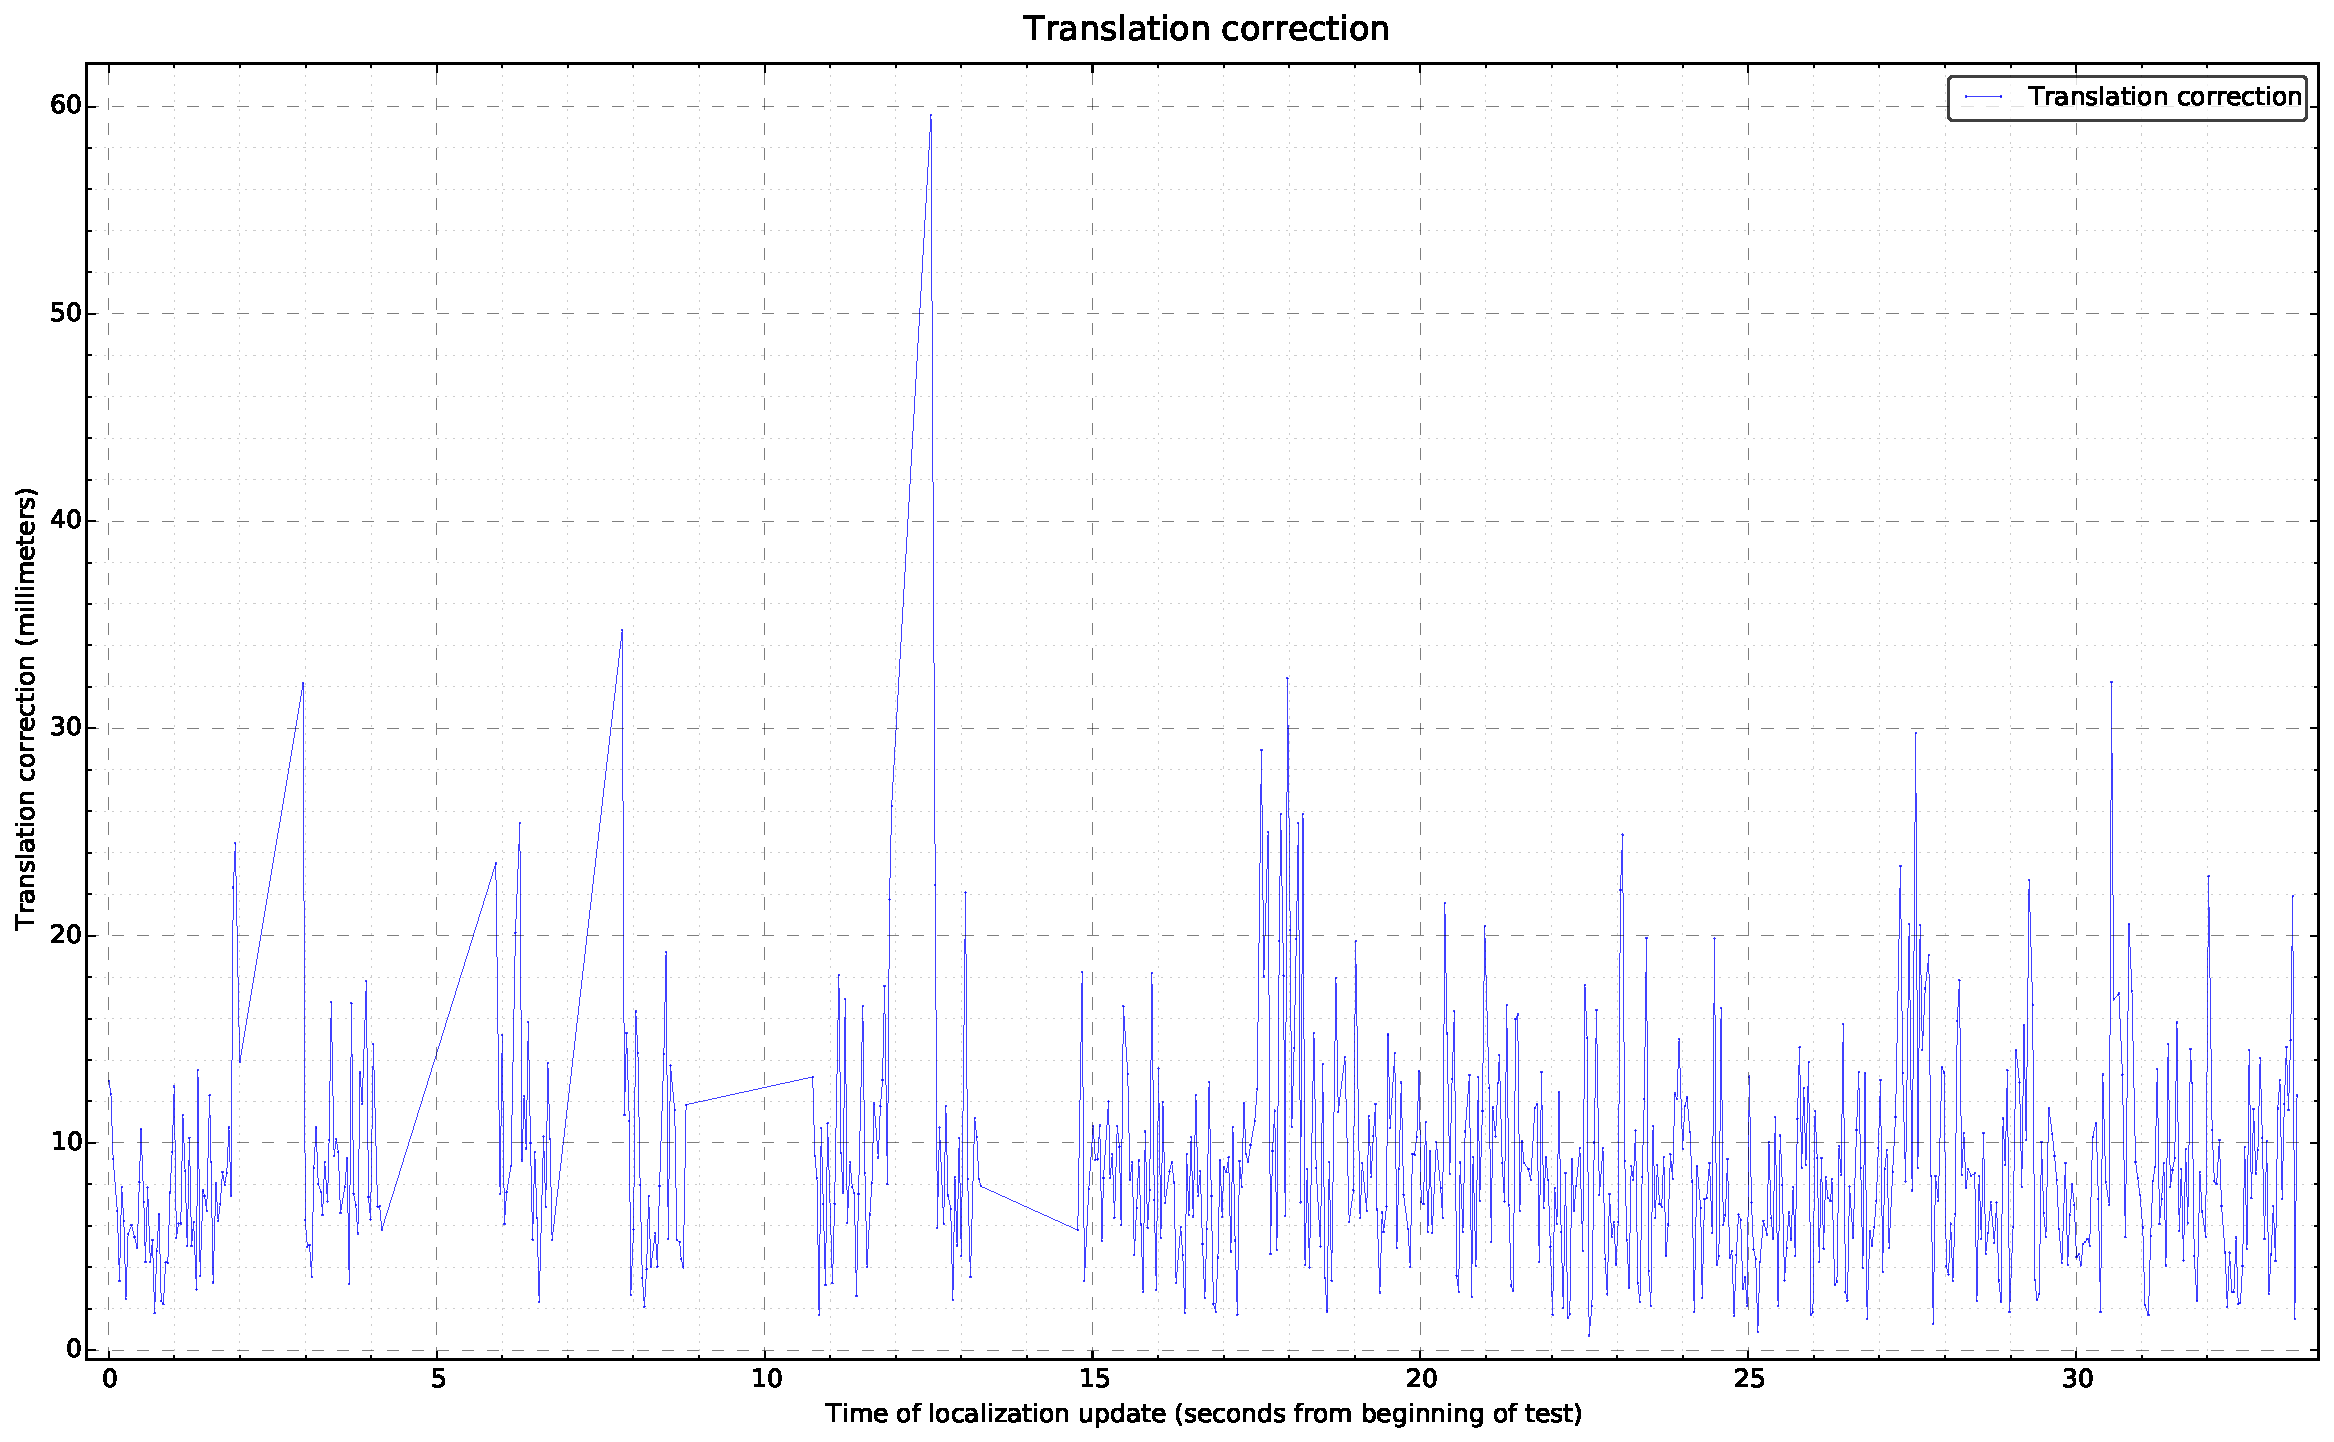
\includegraphics[width=0.69\textwidth]{appendices/tests-3dof/pioneer-robot/\currfilebase/graphs/translation-correction-millimeters}
	\caption{Translation corrections performed by the localization system}
\end{figure}

\begin{figure}[H]
	\centering
	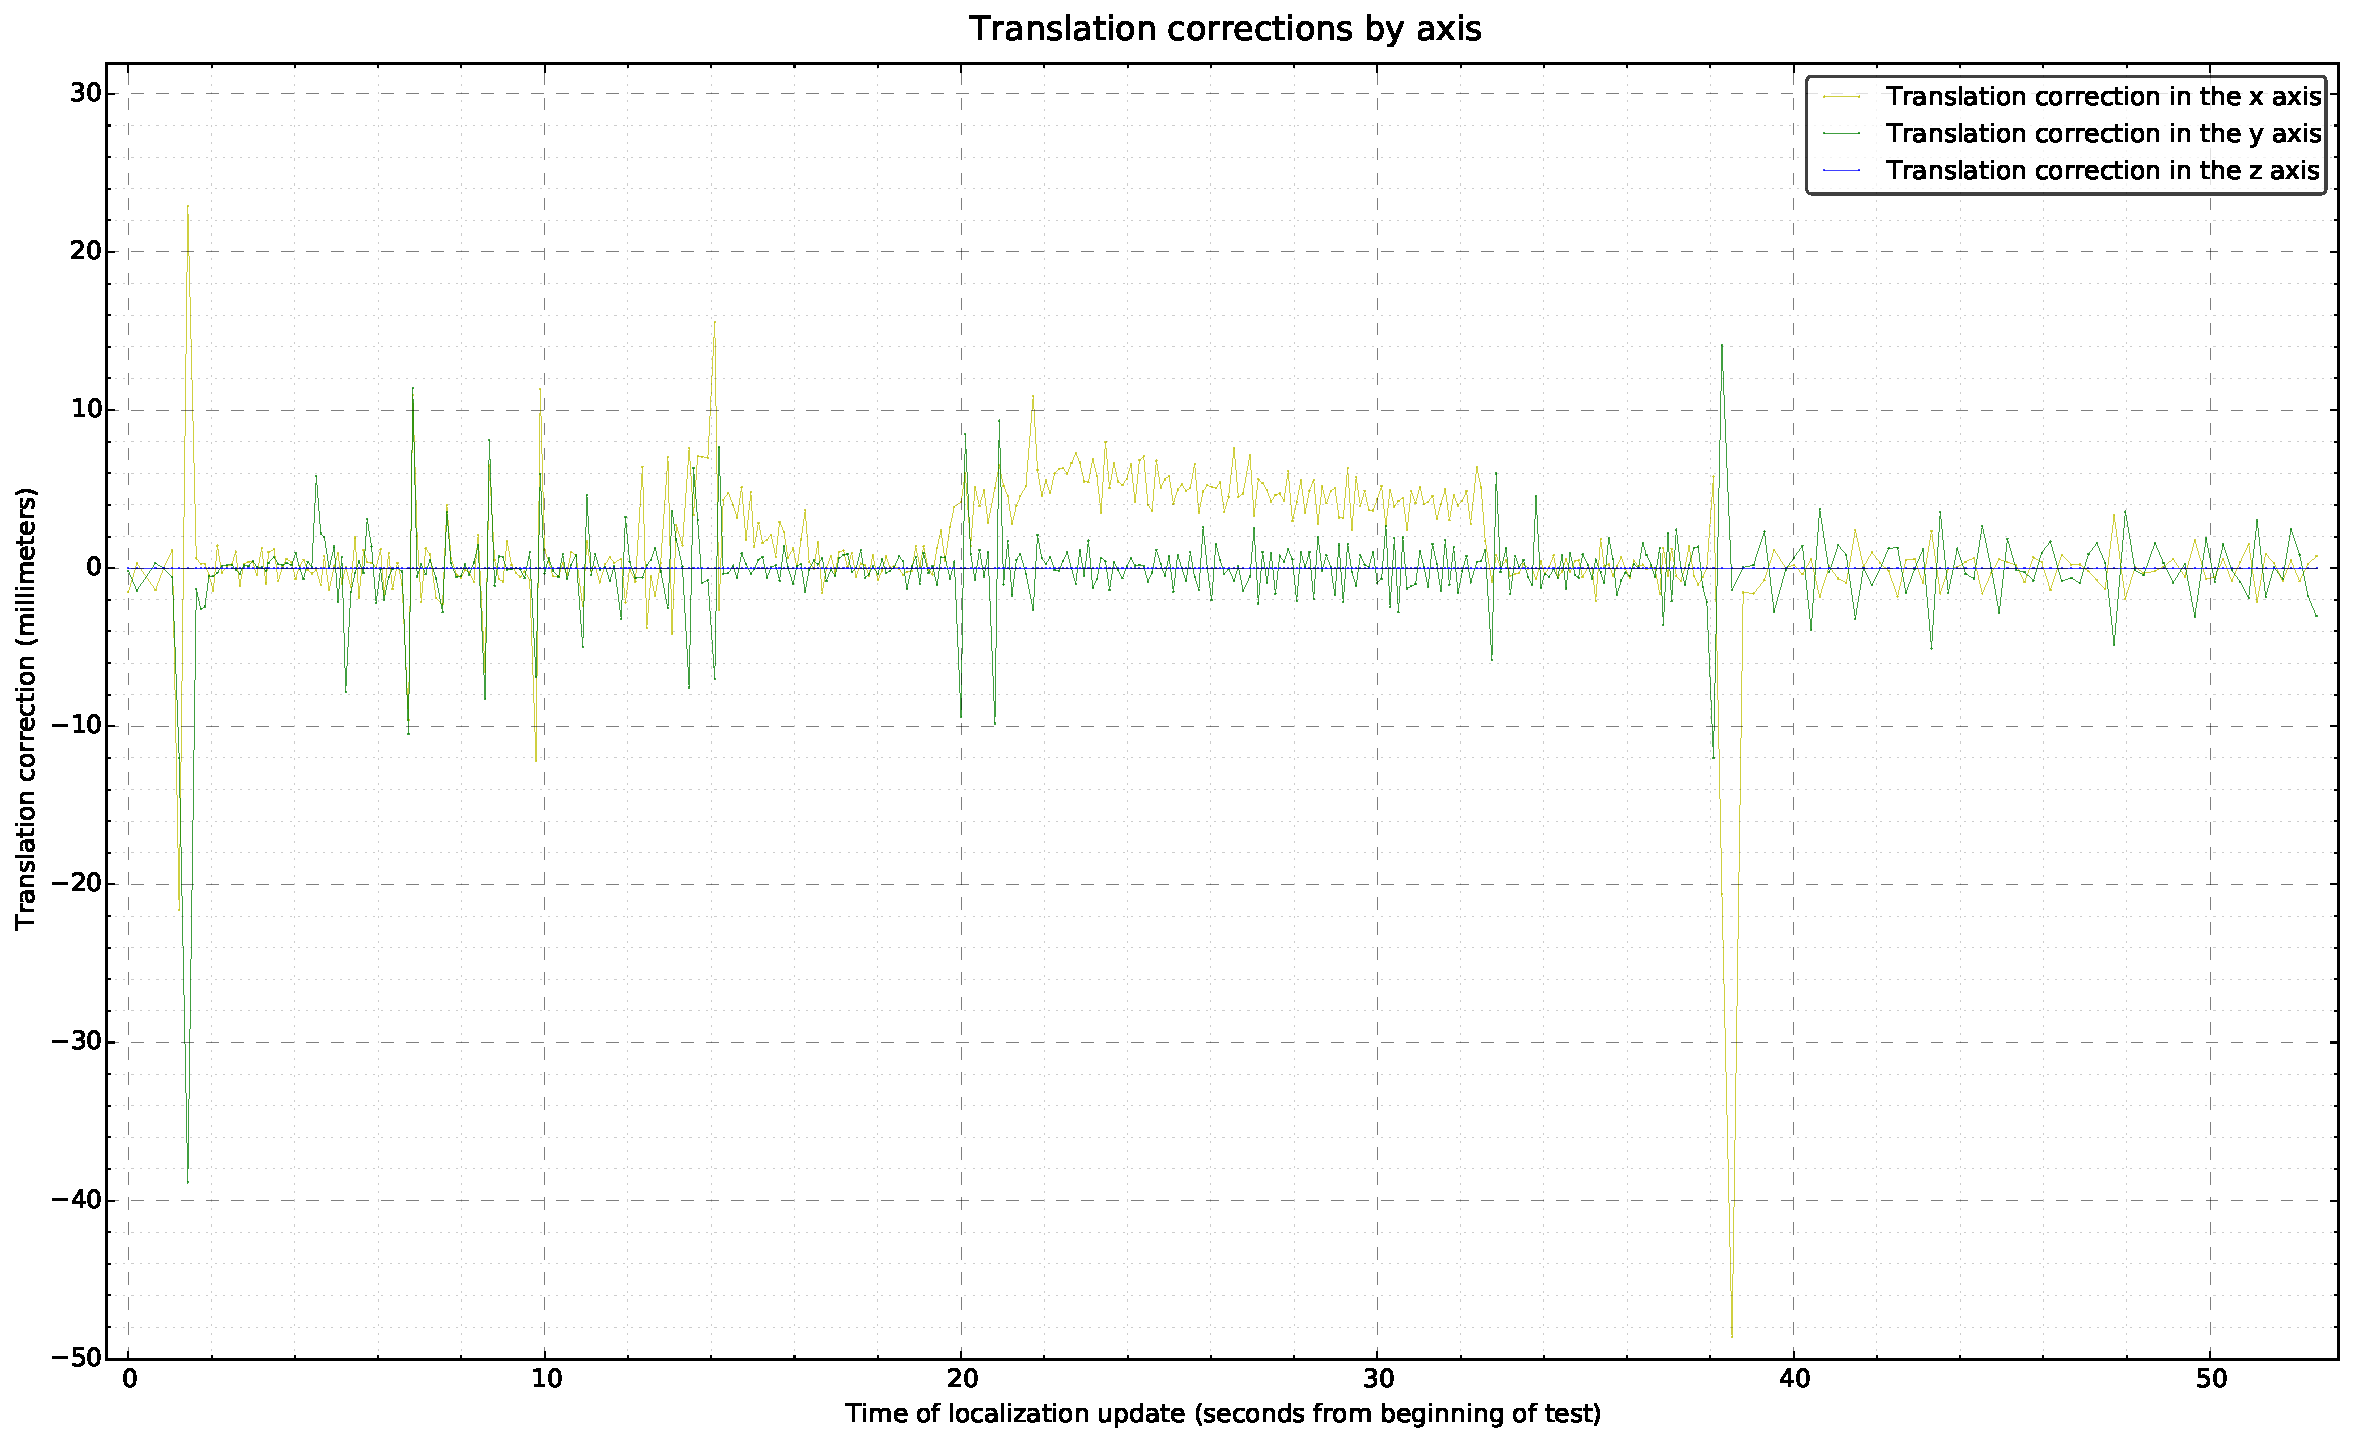
\includegraphics[width=0.69\textwidth]{appendices/tests-3dof/pioneer-robot/\currfilebase/graphs/translation-corrections-components-millimeters}
	\caption{Translation corrections components performed by the localization system}
\end{figure}

\begin{figure}[H]
	\centering
	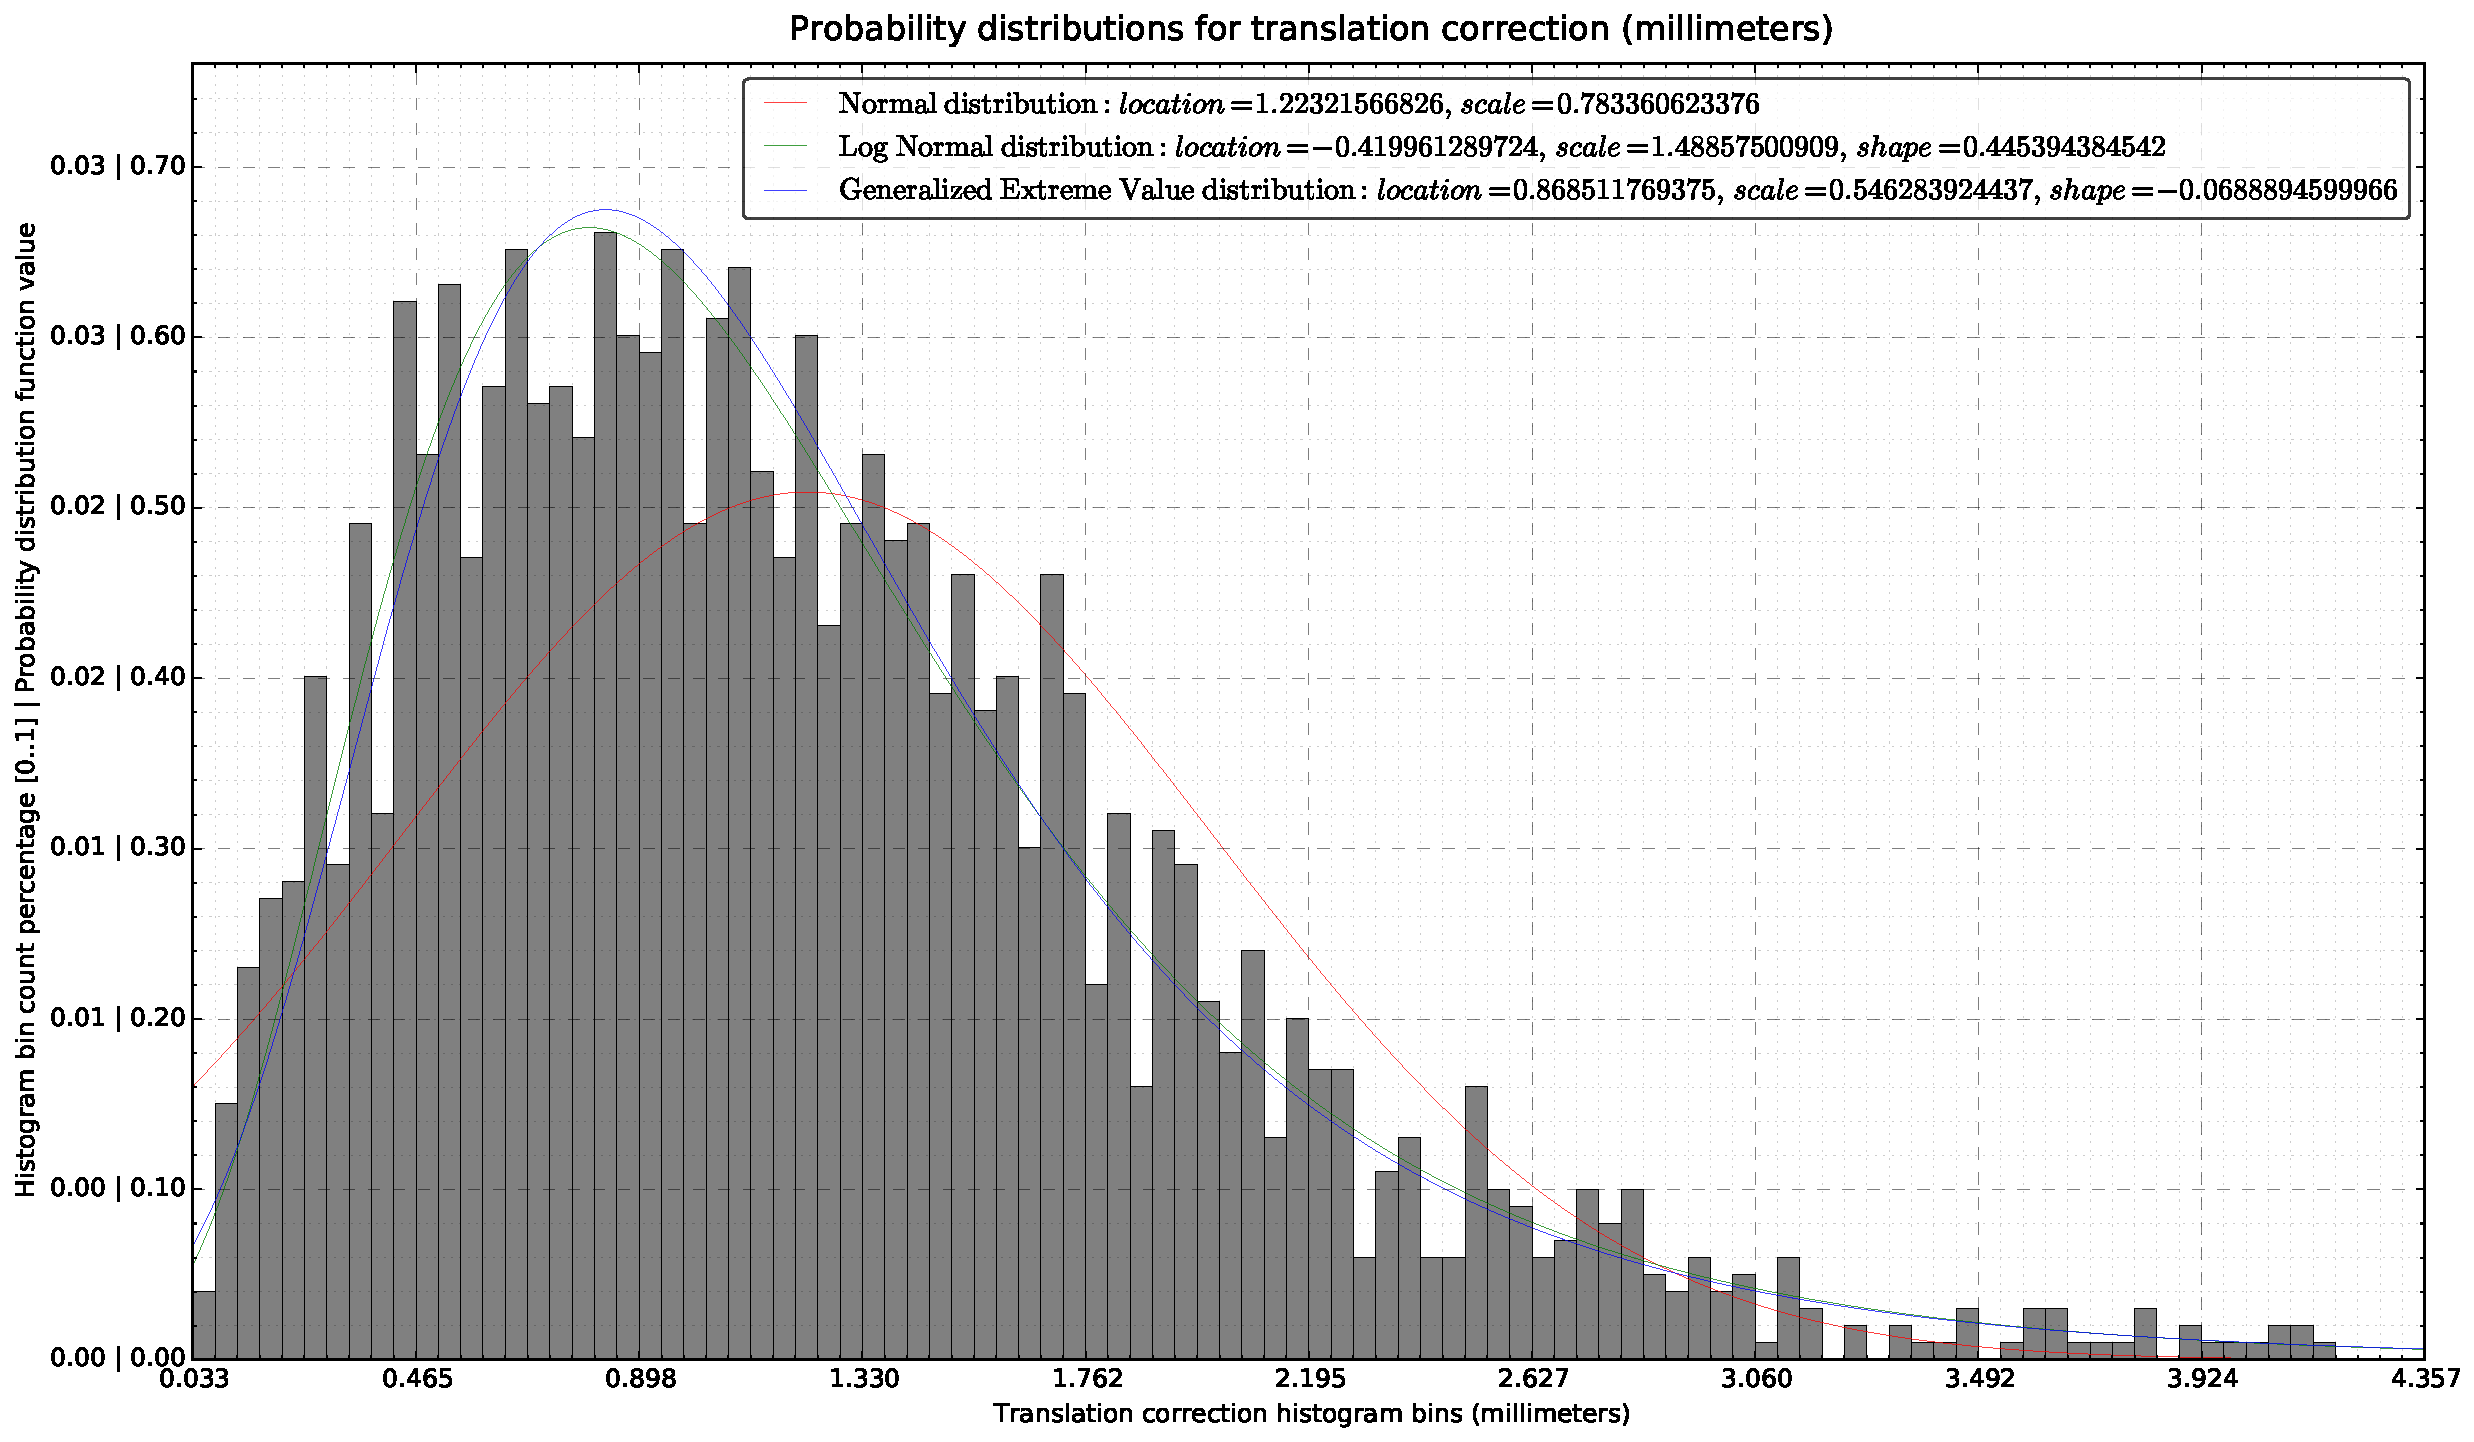
\includegraphics[width=0.69\textwidth]{appendices/tests-3dof/pioneer-robot/\currfilebase/graphs/translation-correction-millimeters-distributions}
	\caption{Probability distributions for the translation corrections performed by the localization system}
\end{figure}


%Rotation corrections axis
\begin{figure}[H]
	\centering
	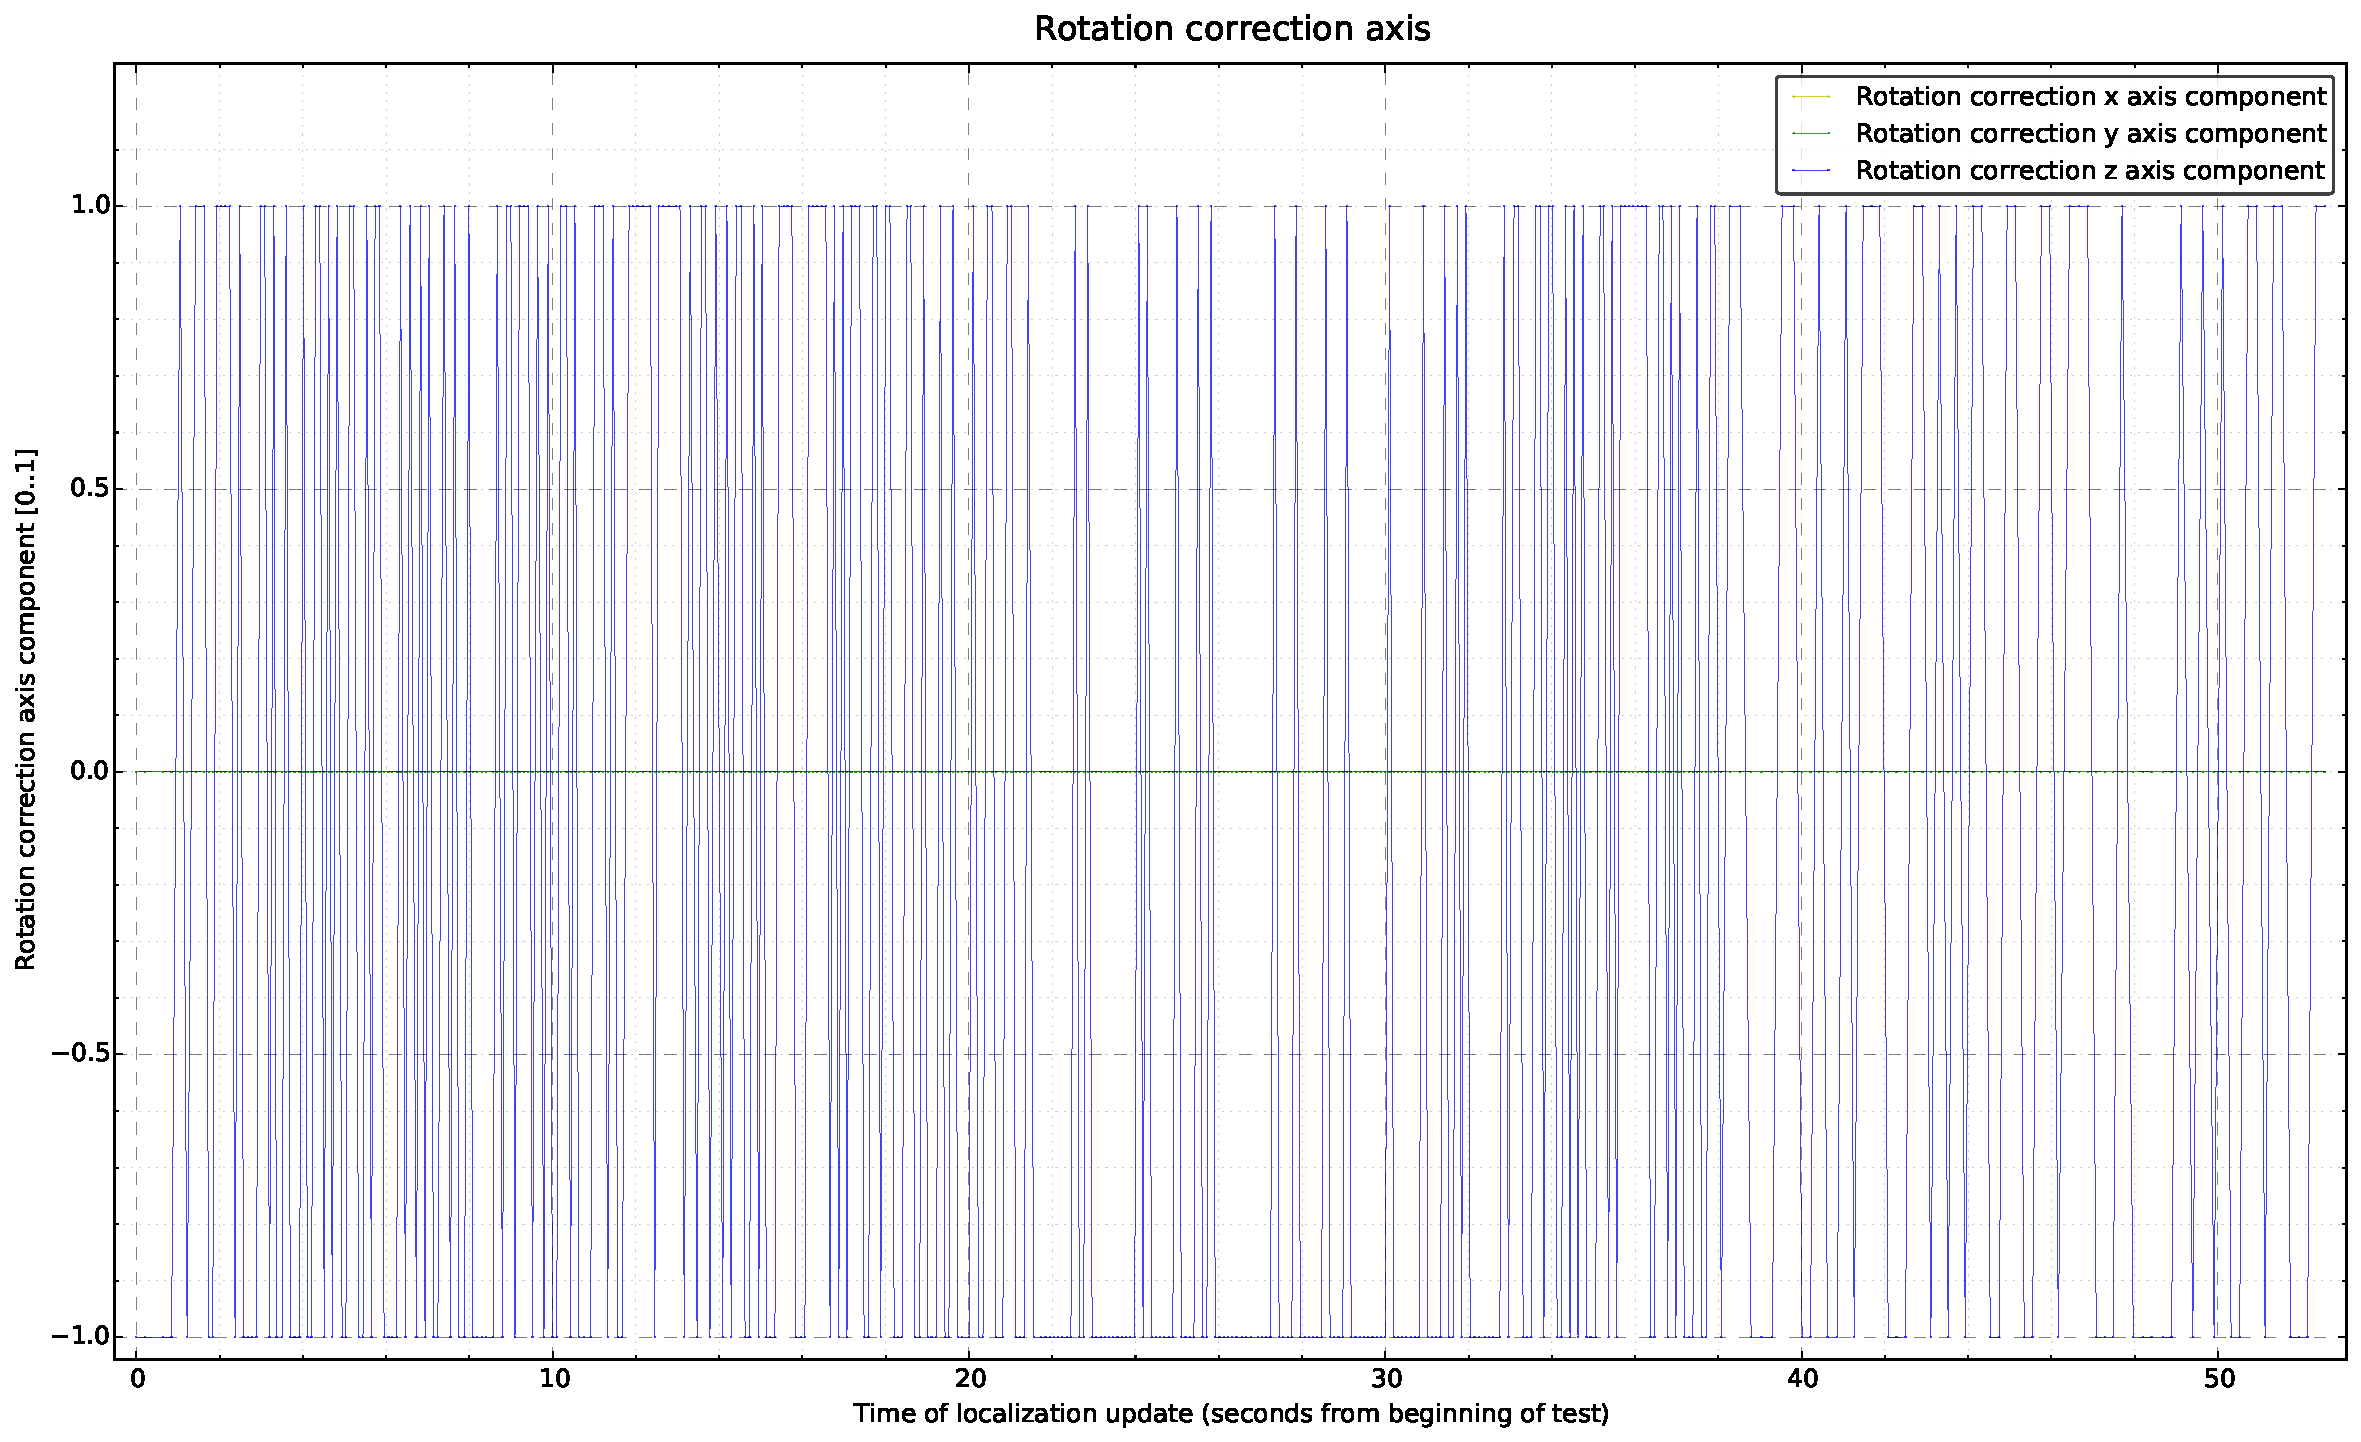
\includegraphics[width=0.69\textwidth]{appendices/tests-3dof/pioneer-robot/\currfilebase/graphs/rotation-correction-axis}
	\caption{Rotation corrections (axis) performed by the localization system}
\end{figure}

\begin{figure}[H]
	\centering
	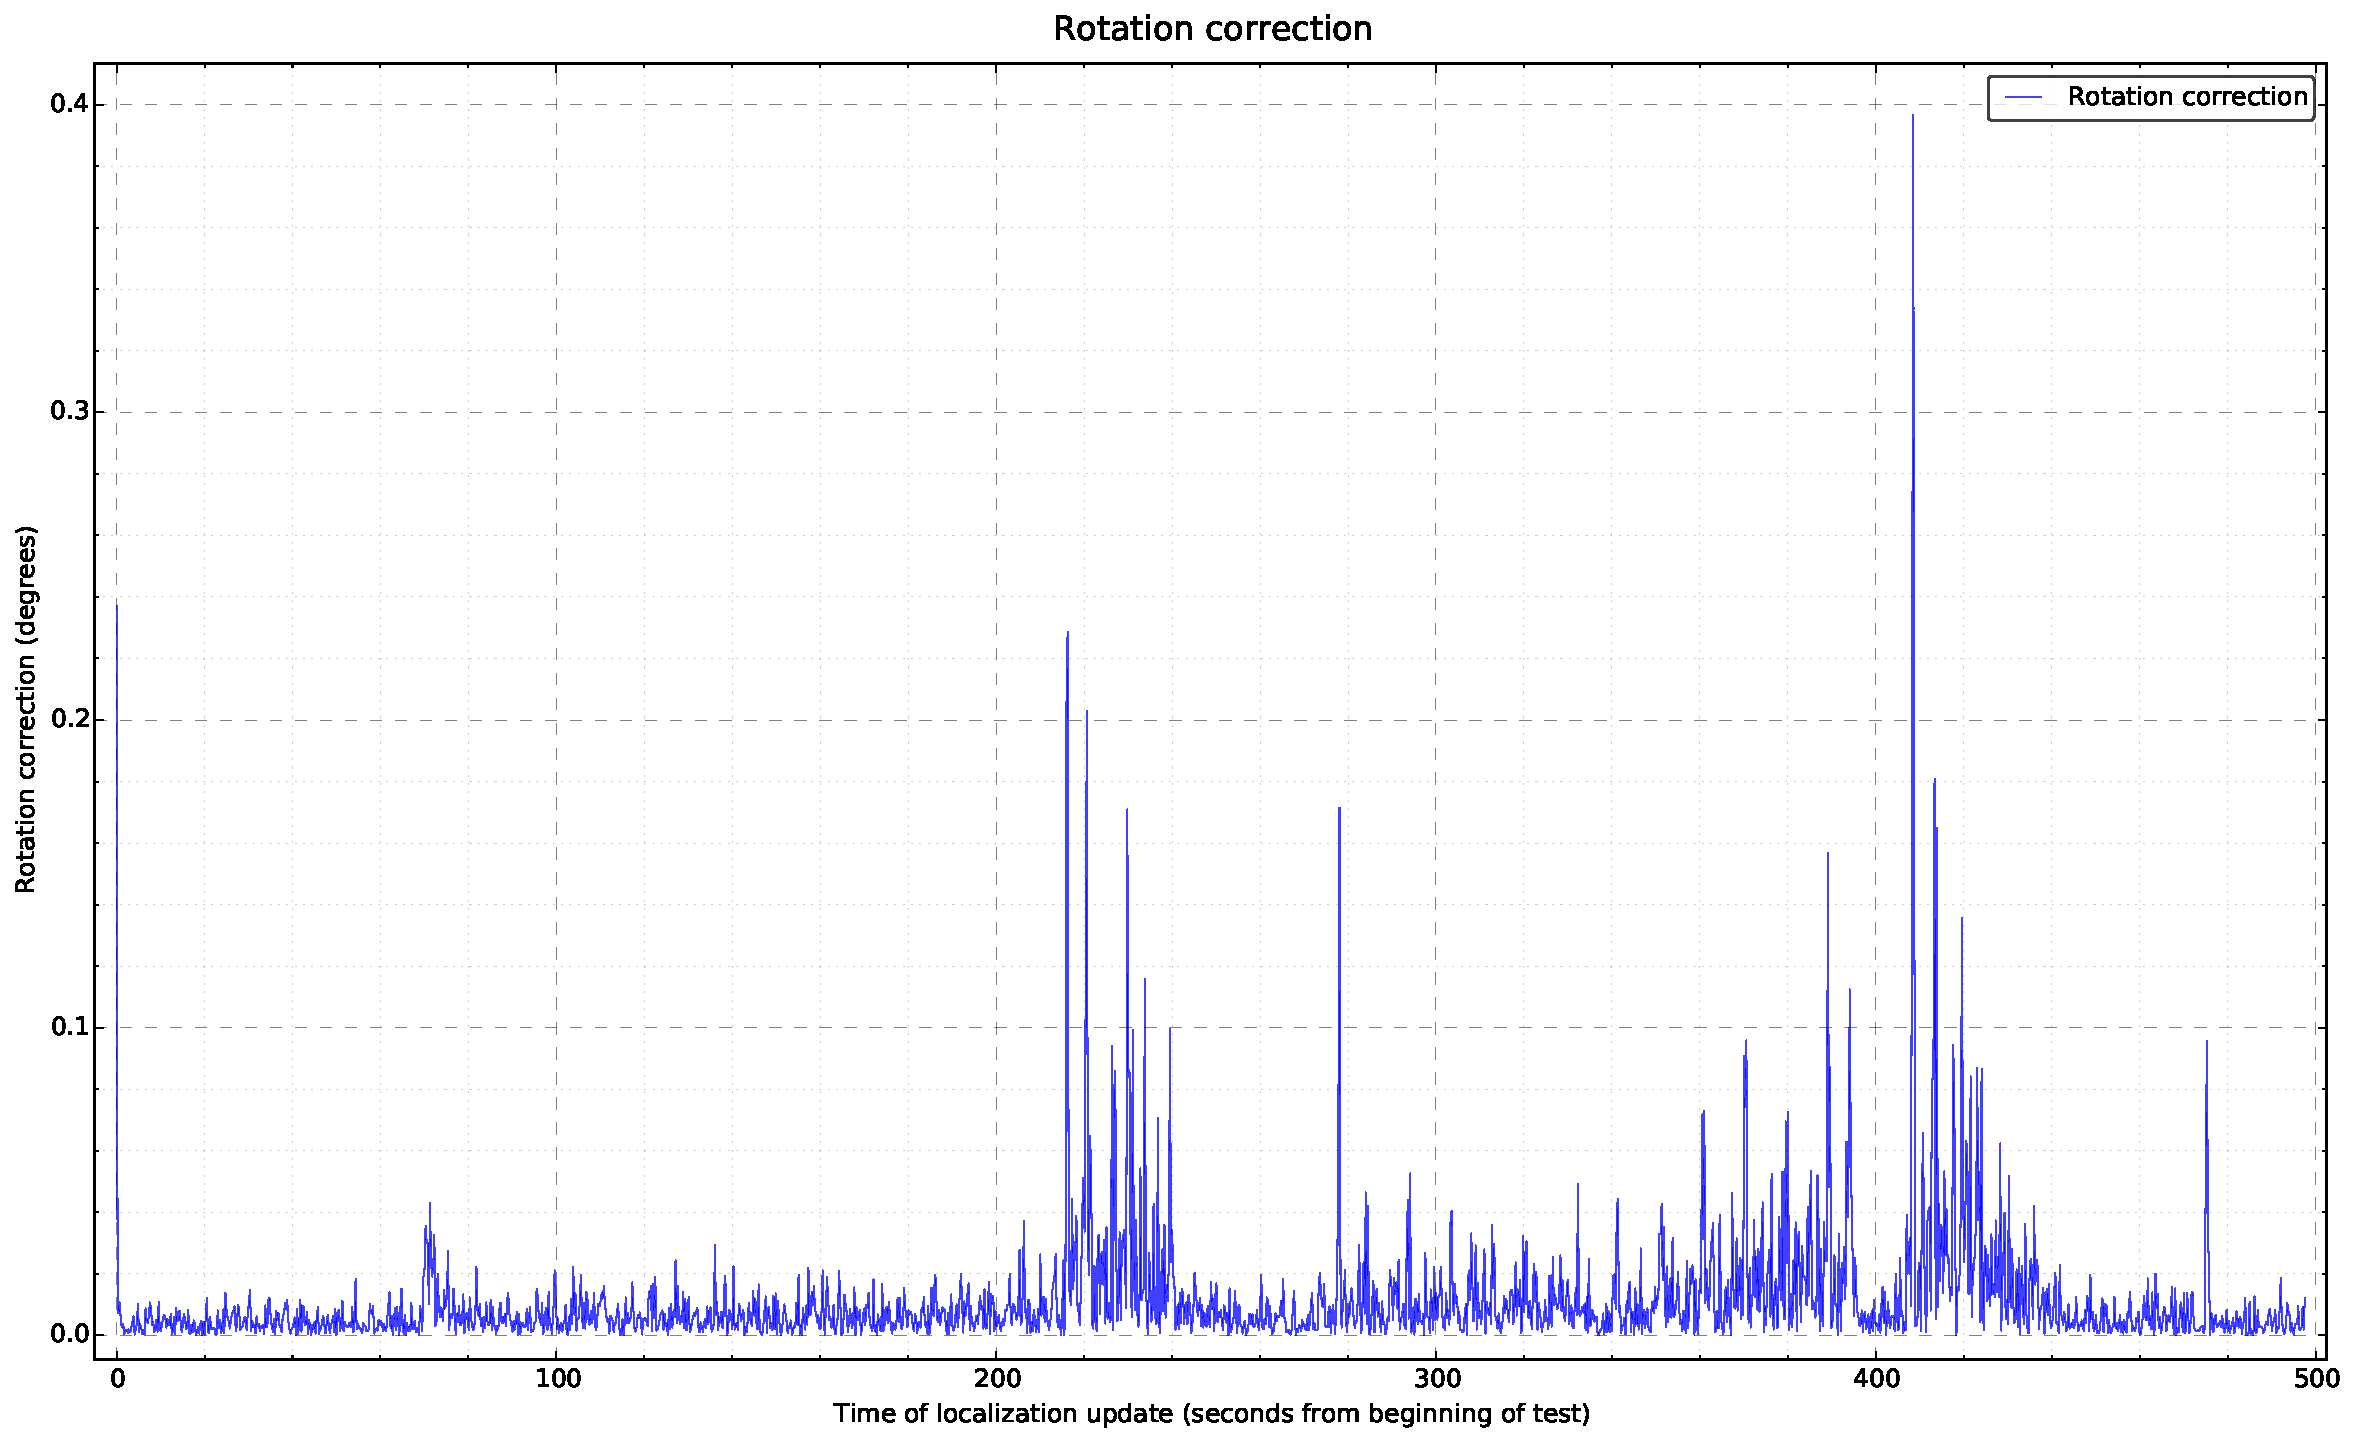
\includegraphics[width=0.69\textwidth]{appendices/tests-3dof/pioneer-robot/\currfilebase/graphs/rotation-correction-degrees}
	\caption{Rotation corrections performed by the localization system}
\end{figure}

\begin{figure}[H]
	\centering
	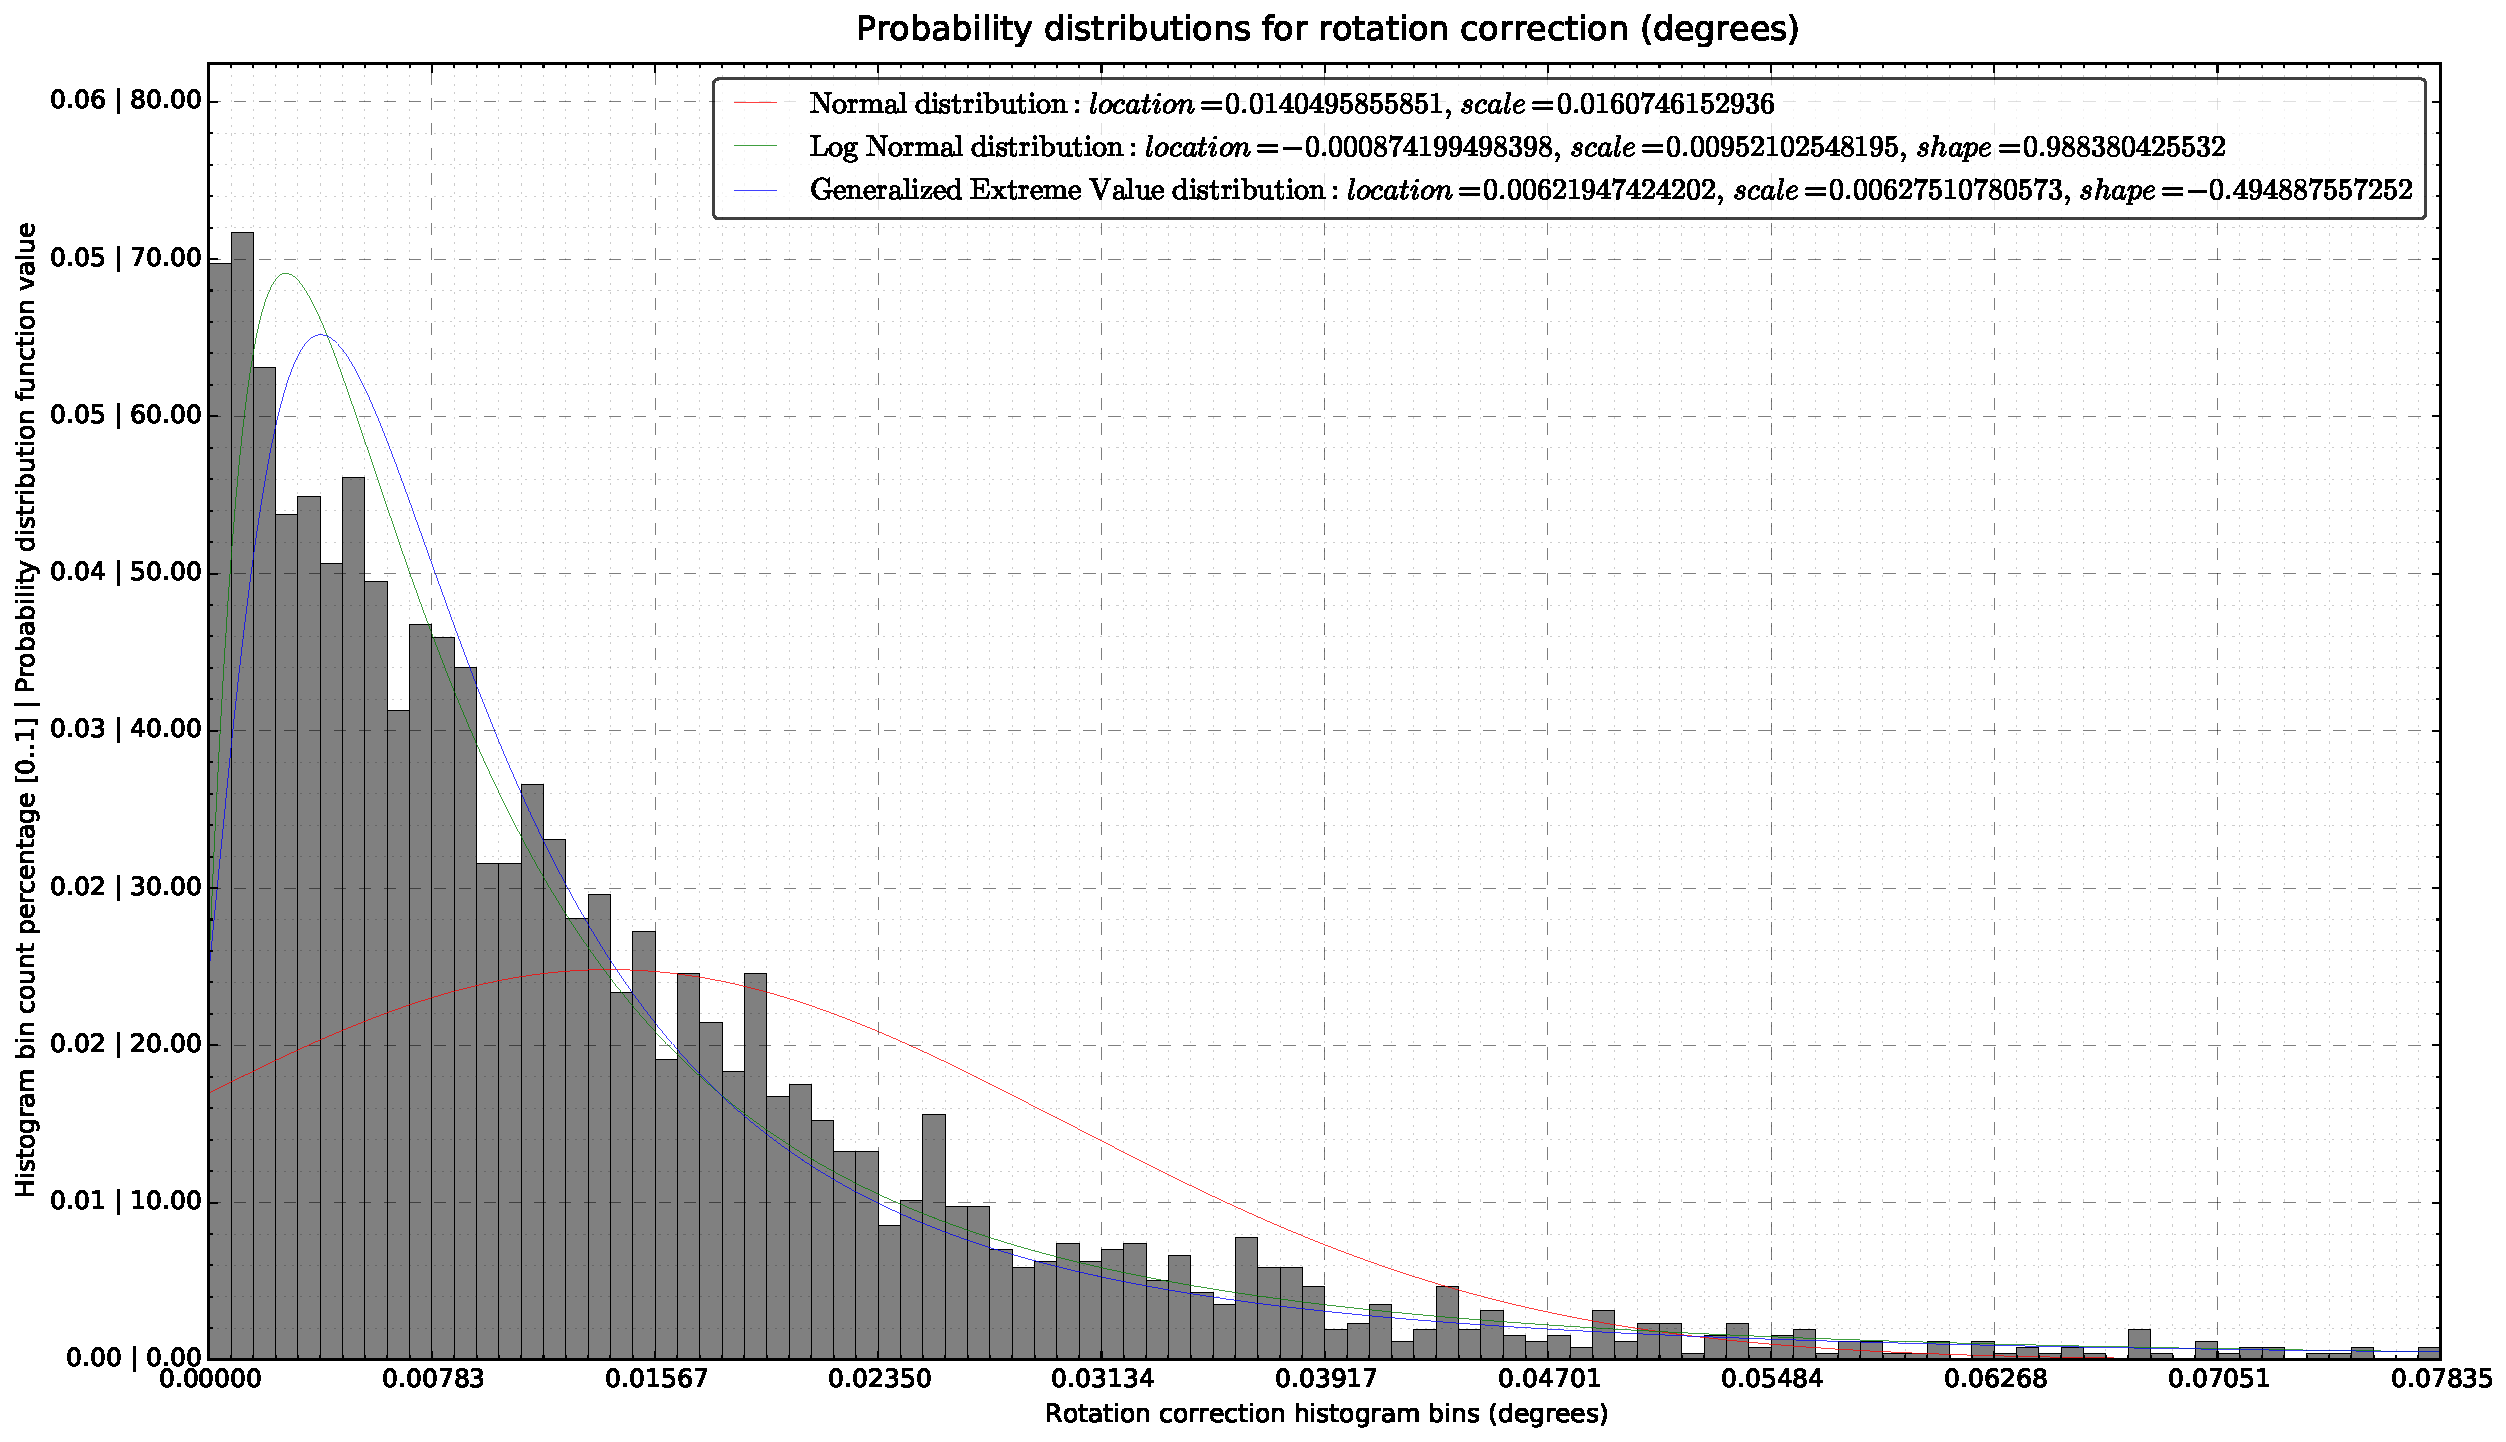
\includegraphics[width=0.69\textwidth]{appendices/tests-3dof/pioneer-robot/\currfilebase/graphs/rotation-correction-degrees-distributions}
	\caption{Probability distributions for the rotation corrections performed by the localization system}
\end{figure}


%Registered points (inliers / outliers)
\begin{figure}[H]
	\centering
	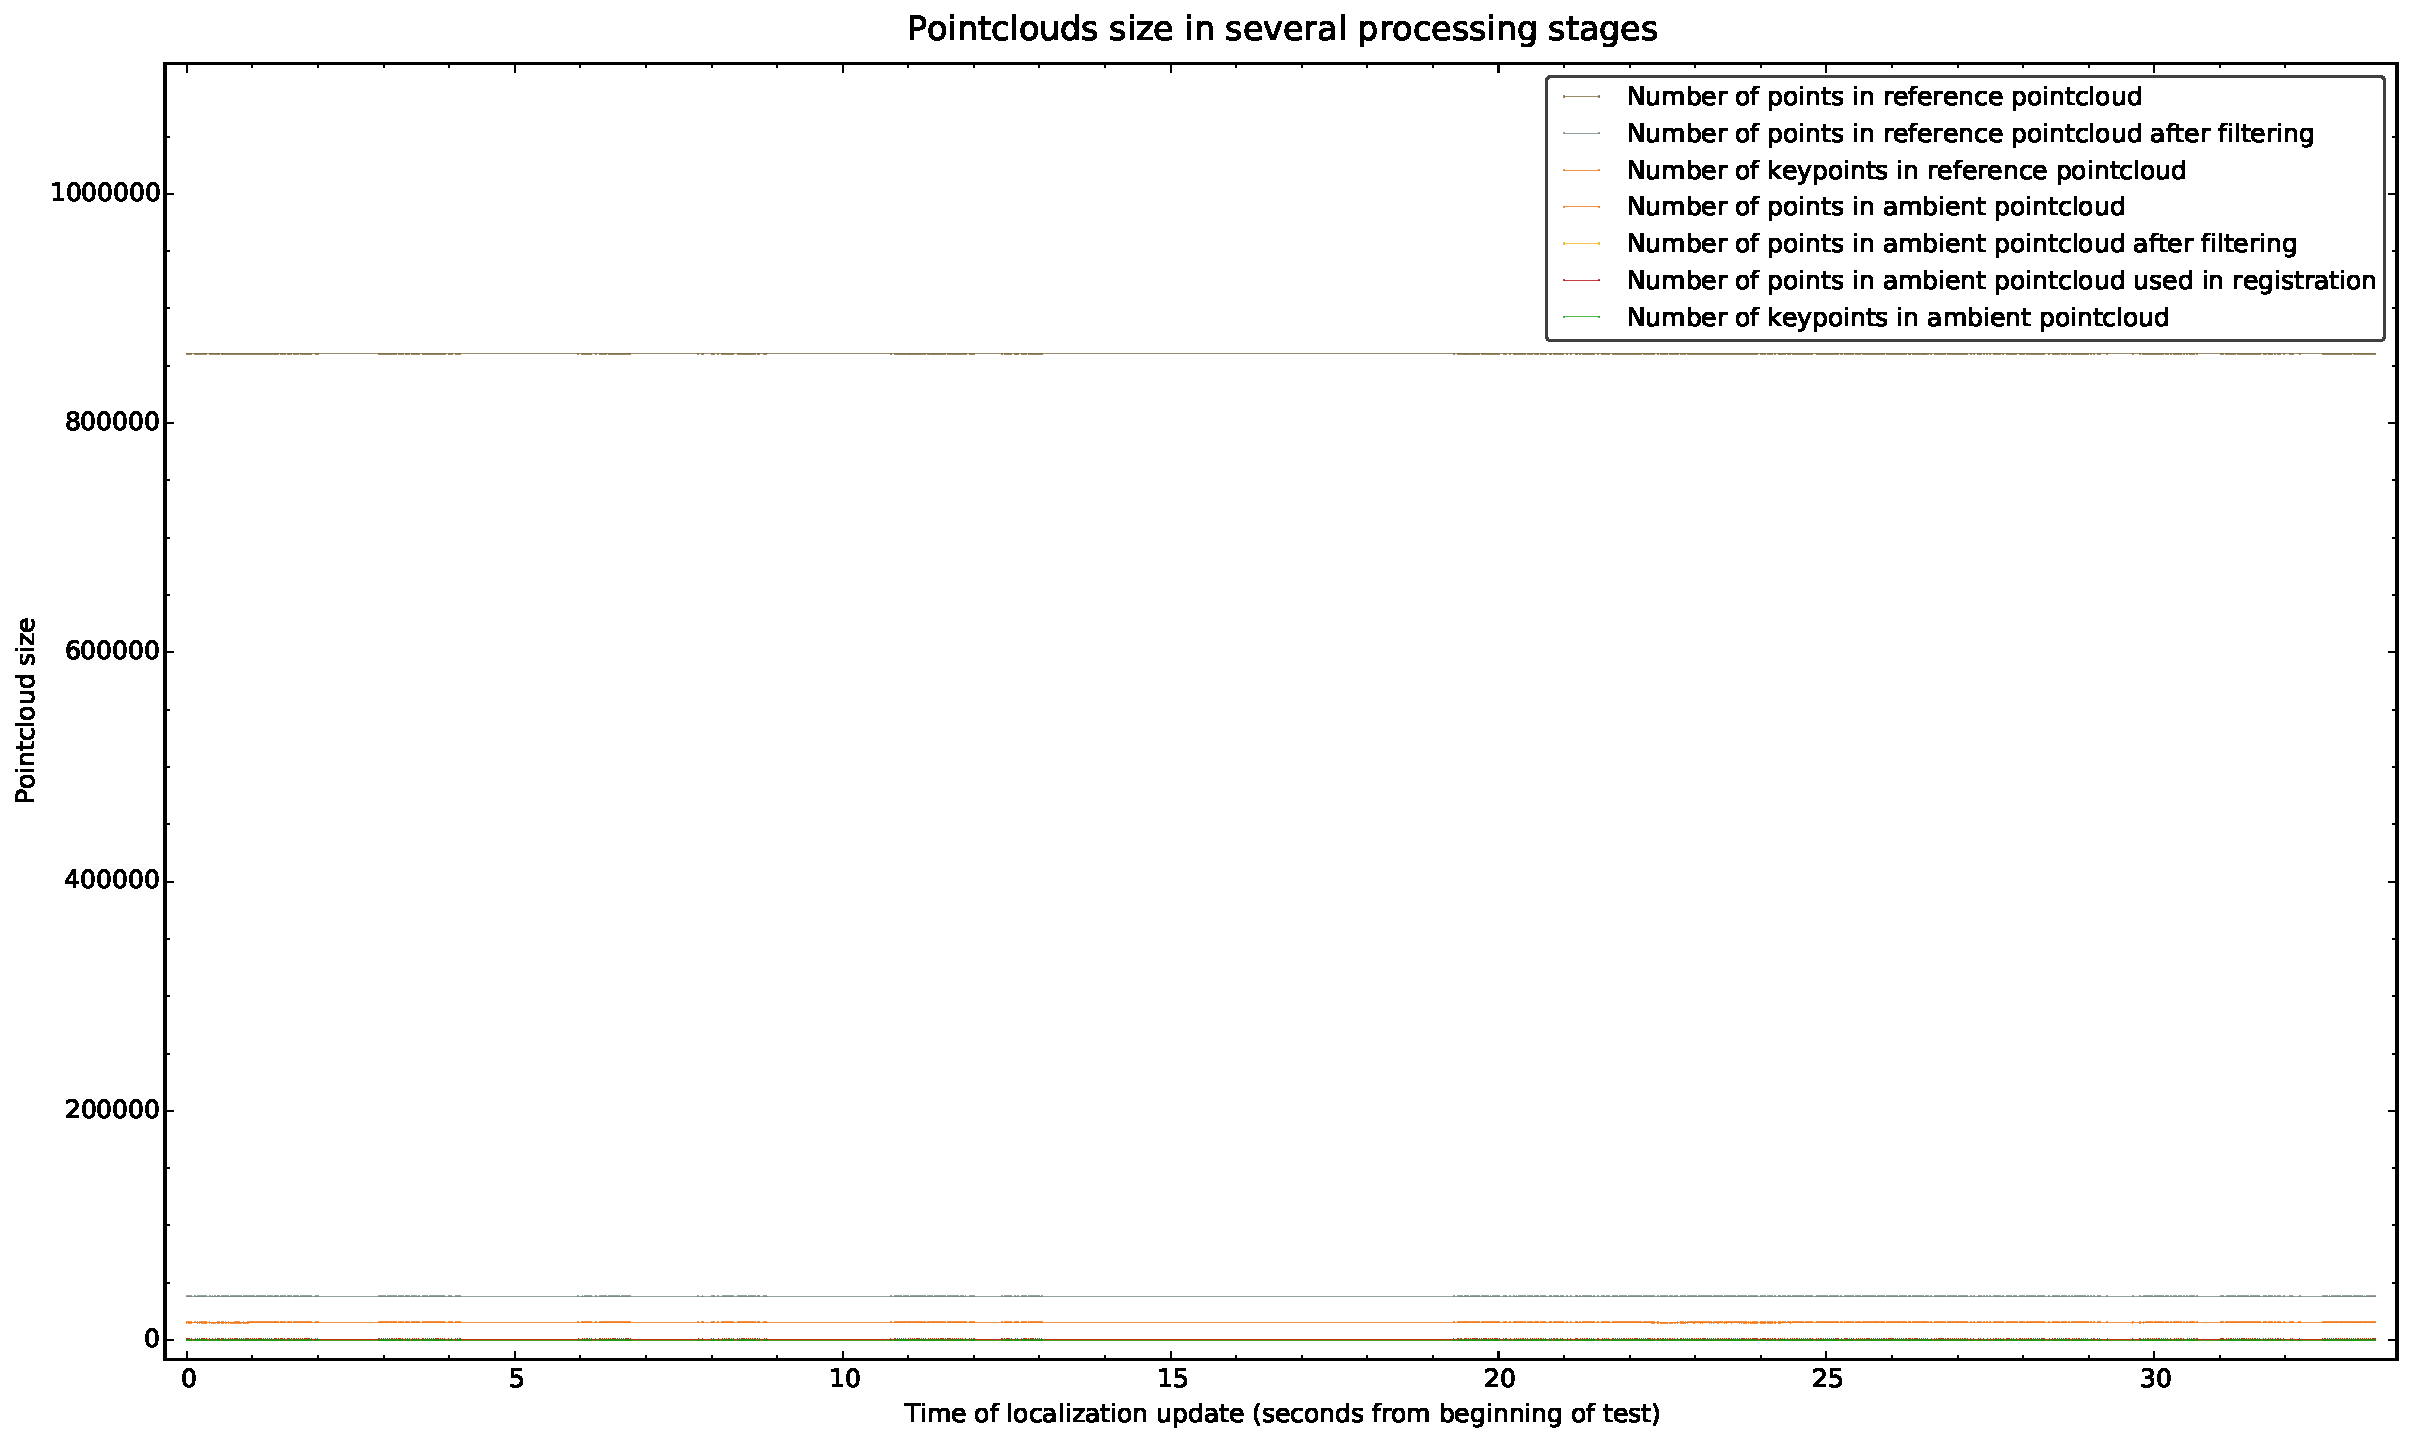
\includegraphics[width=0.69\textwidth]{appendices/tests-3dof/pioneer-robot/\currfilebase/graphs/pointclouds-size}
	\caption{Point clouds size in several of the localization system processing stages}
\end{figure}

\begin{figure}[H]
	\centering
	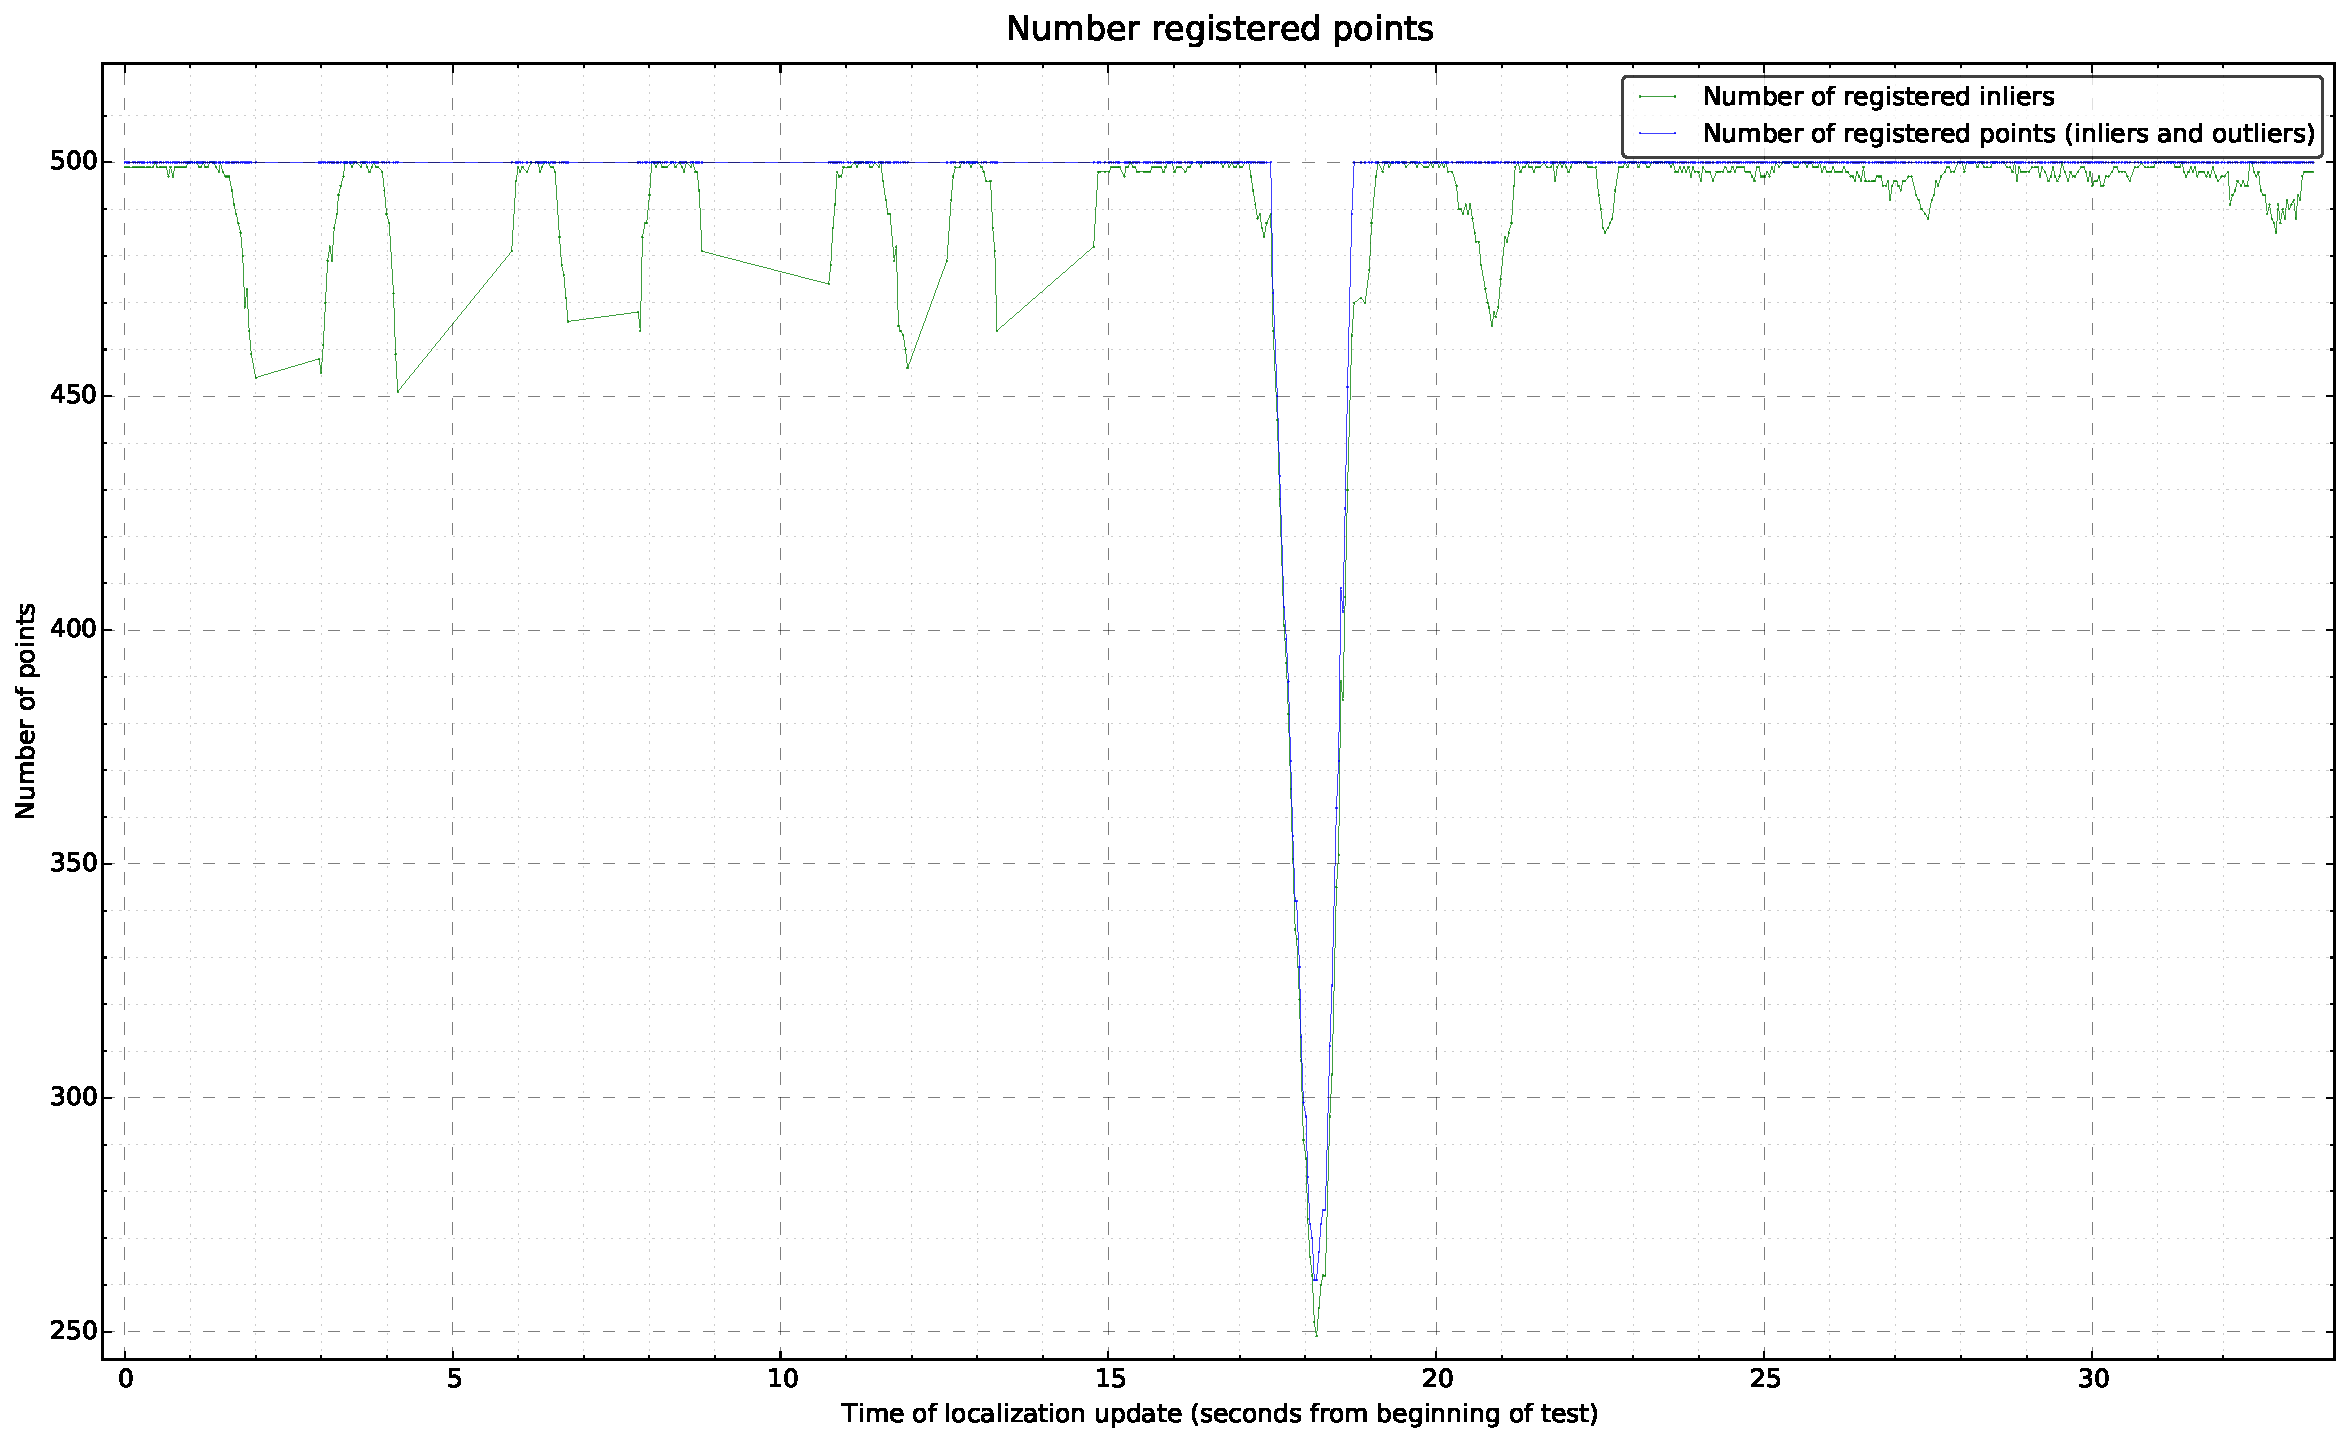
\includegraphics[width=0.69\textwidth]{appendices/tests-3dof/pioneer-robot/\currfilebase/graphs/registered-points}
	\caption{Number of registered points}
\end{figure}

\begin{figure}[H]
	\centering
	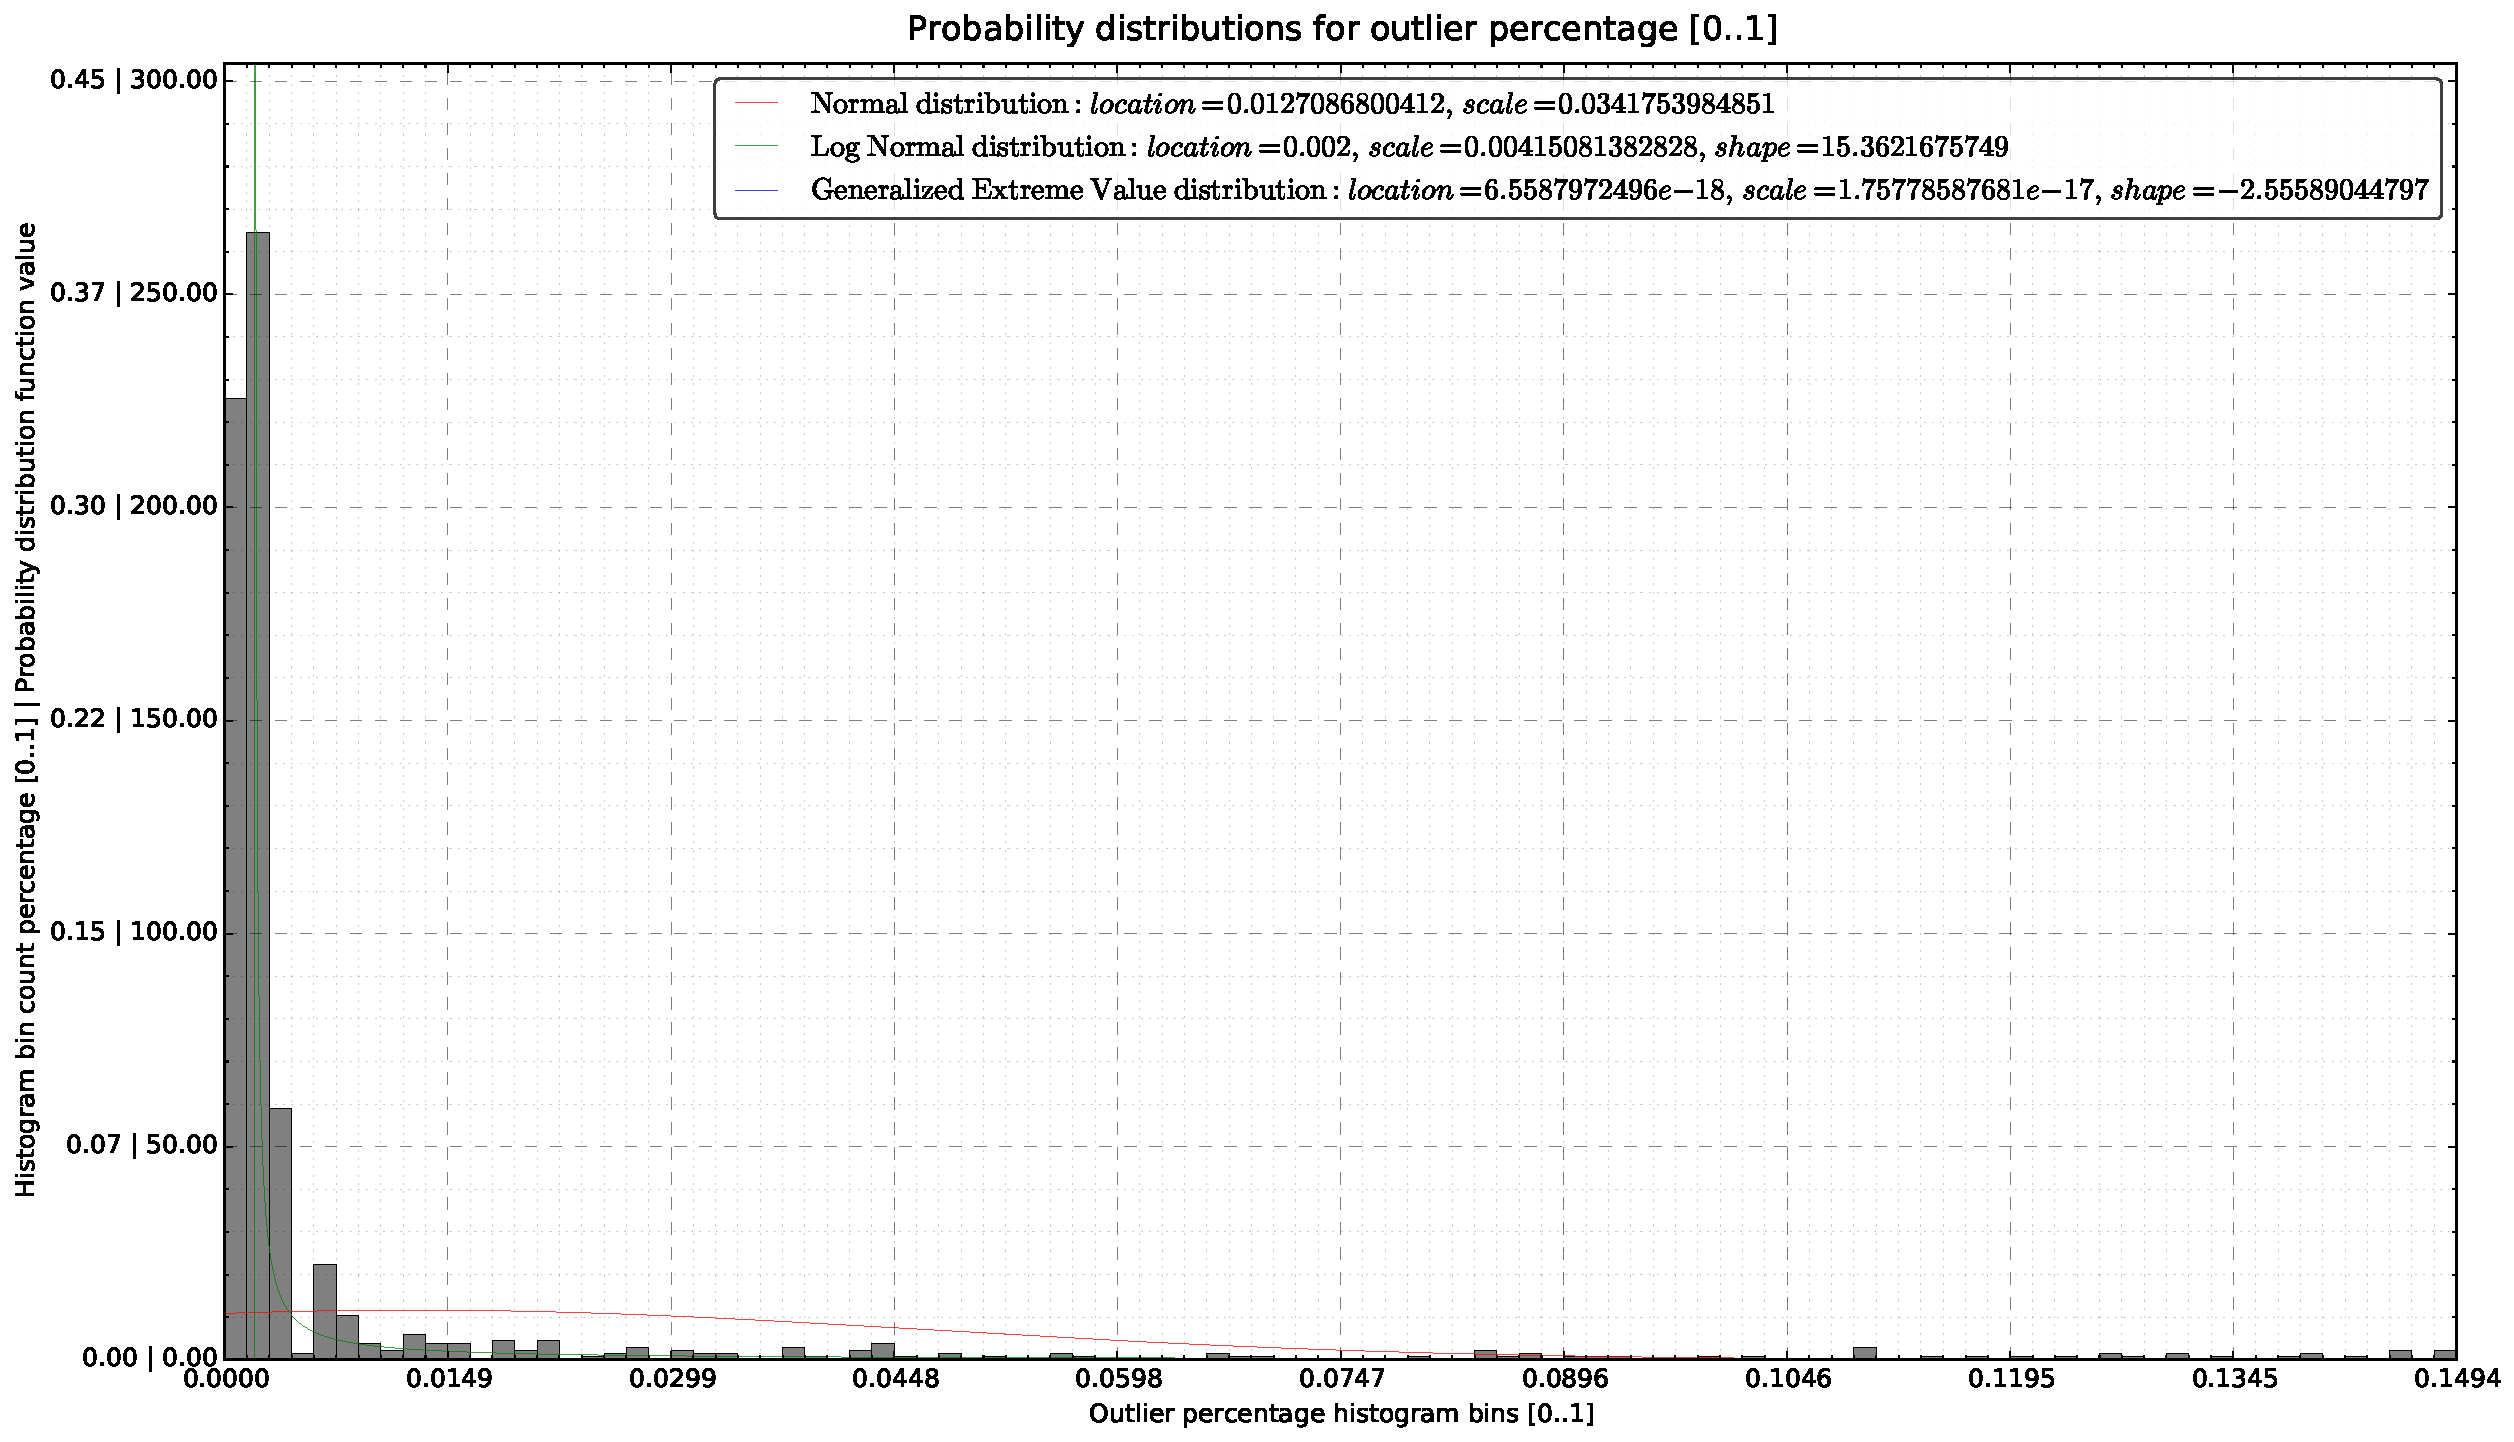
\includegraphics[width=0.69\textwidth]{appendices/tests-3dof/pioneer-robot/\currfilebase/graphs/outlier-percentage-distributions}
	\caption{Probability distributions for the ambient point cloud outlier percentage}
\end{figure}


\begin{figure}[H]
	\centering
	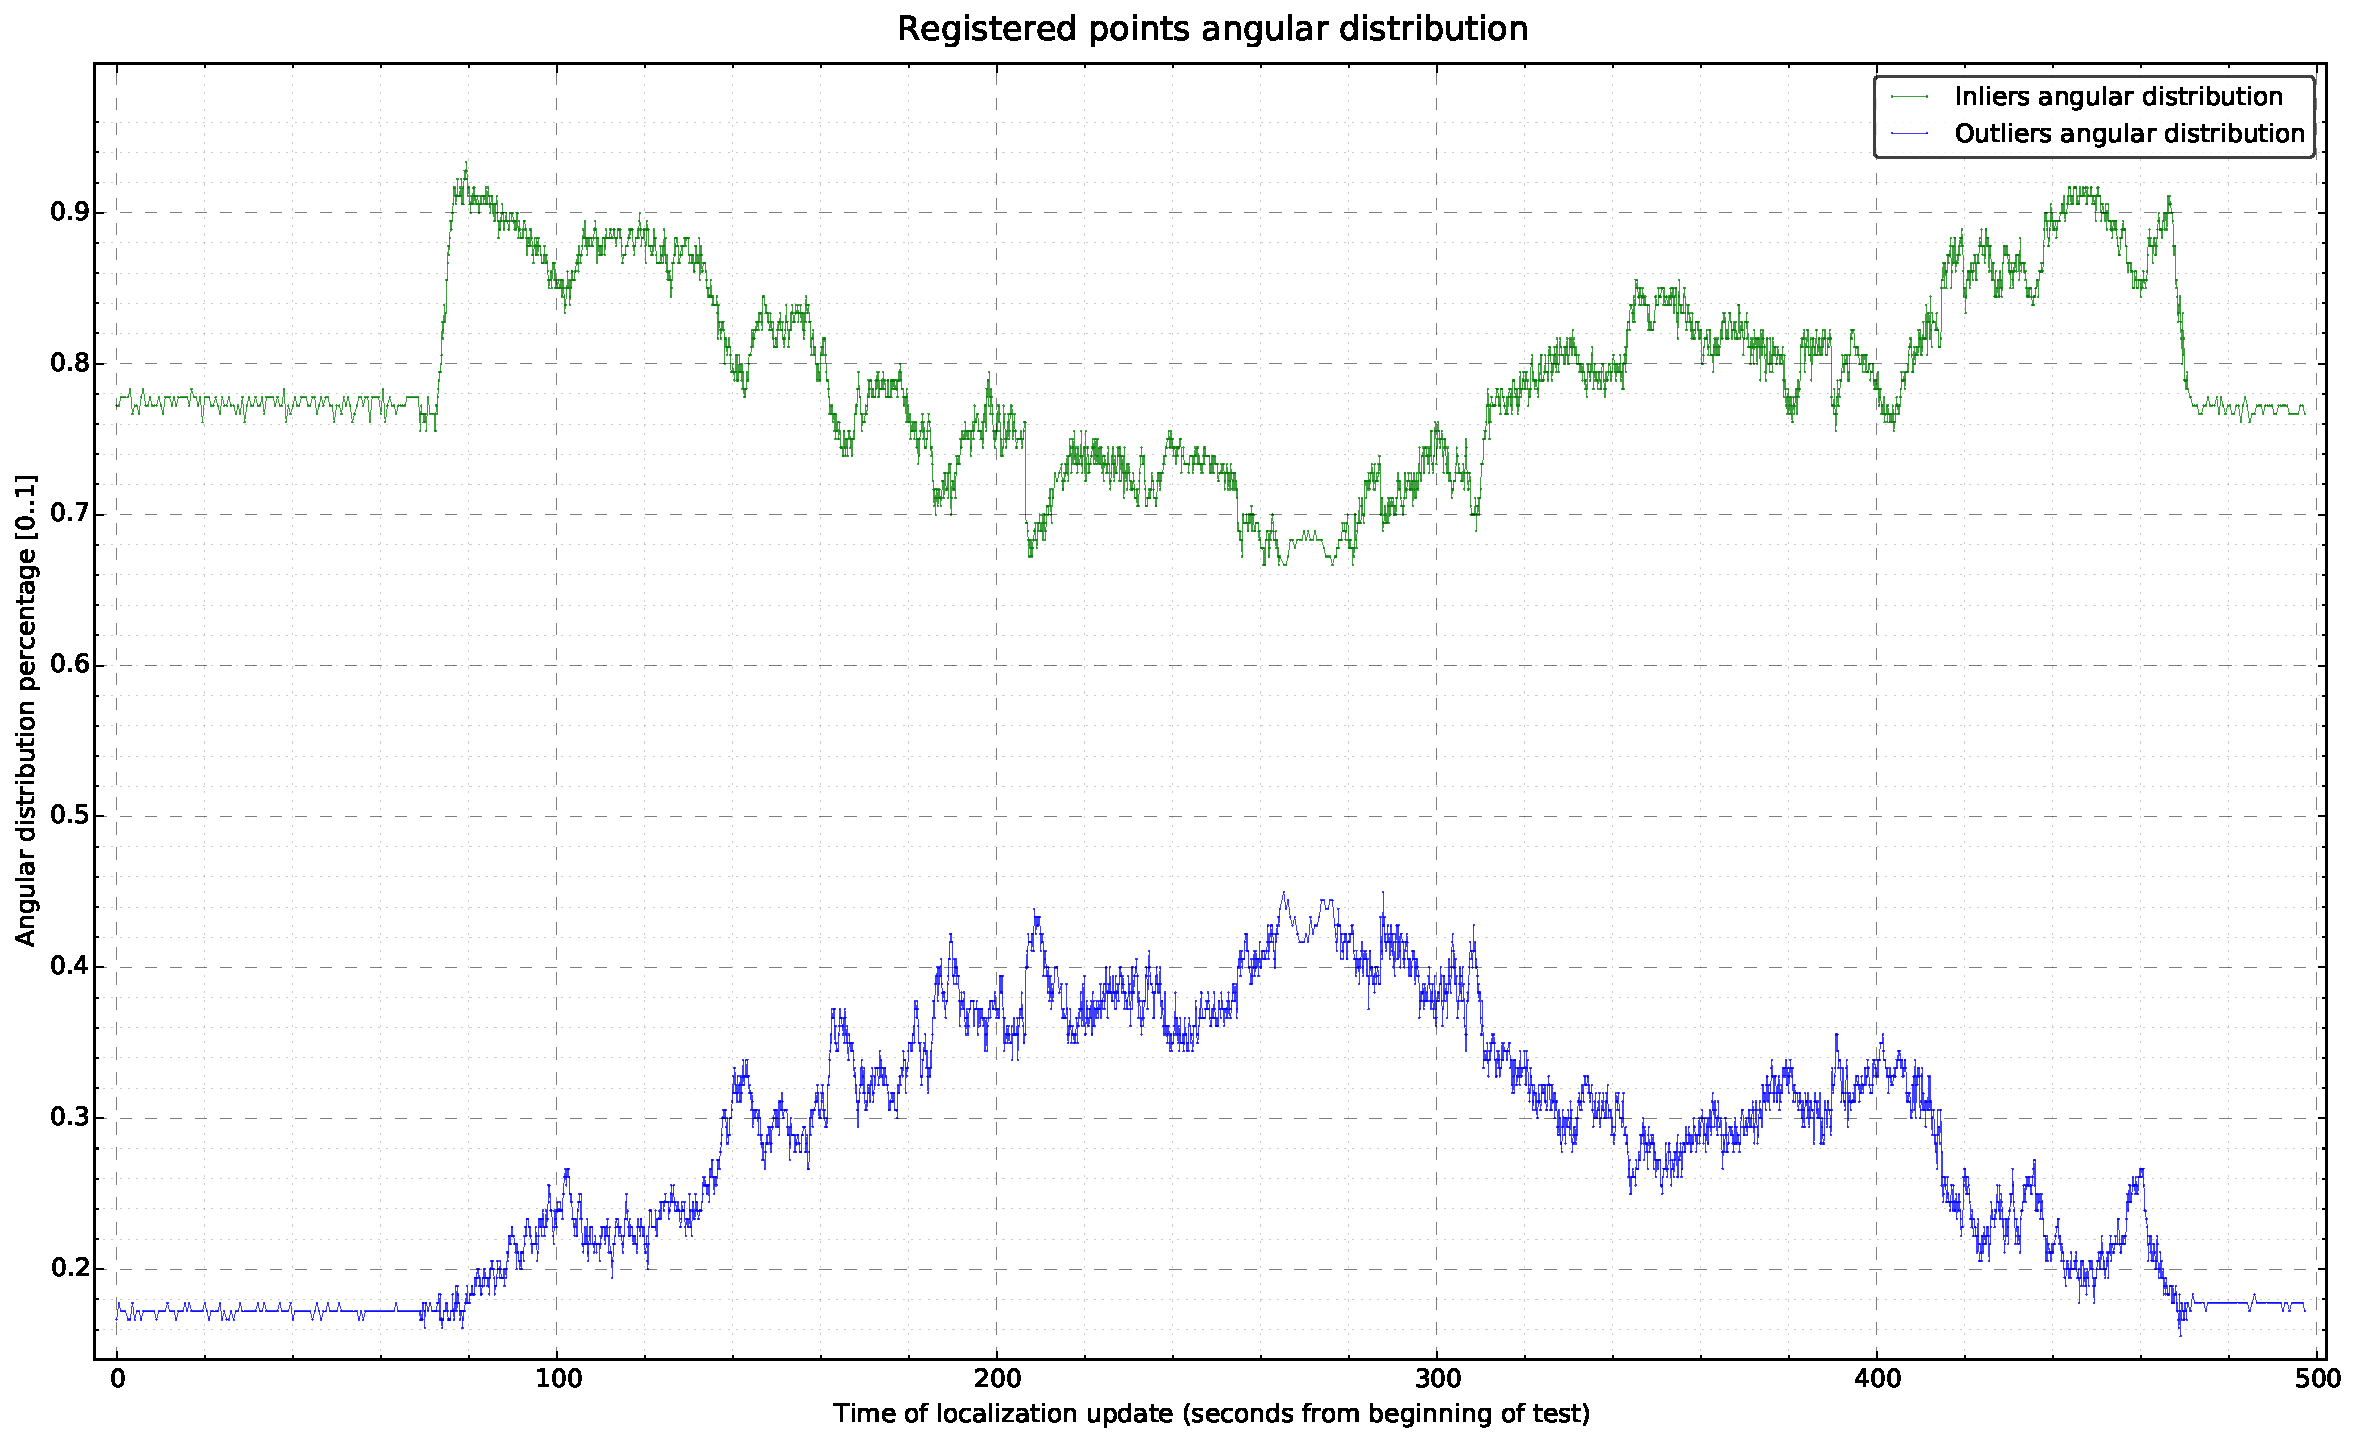
\includegraphics[width=0.69\textwidth]{appendices/tests-3dof/pioneer-robot/\currfilebase/graphs/registered-points-angular-distribution}
	\caption{Angular distribution percentage of registered points}
\end{figure}

\begin{figure}[H]
	\centering
	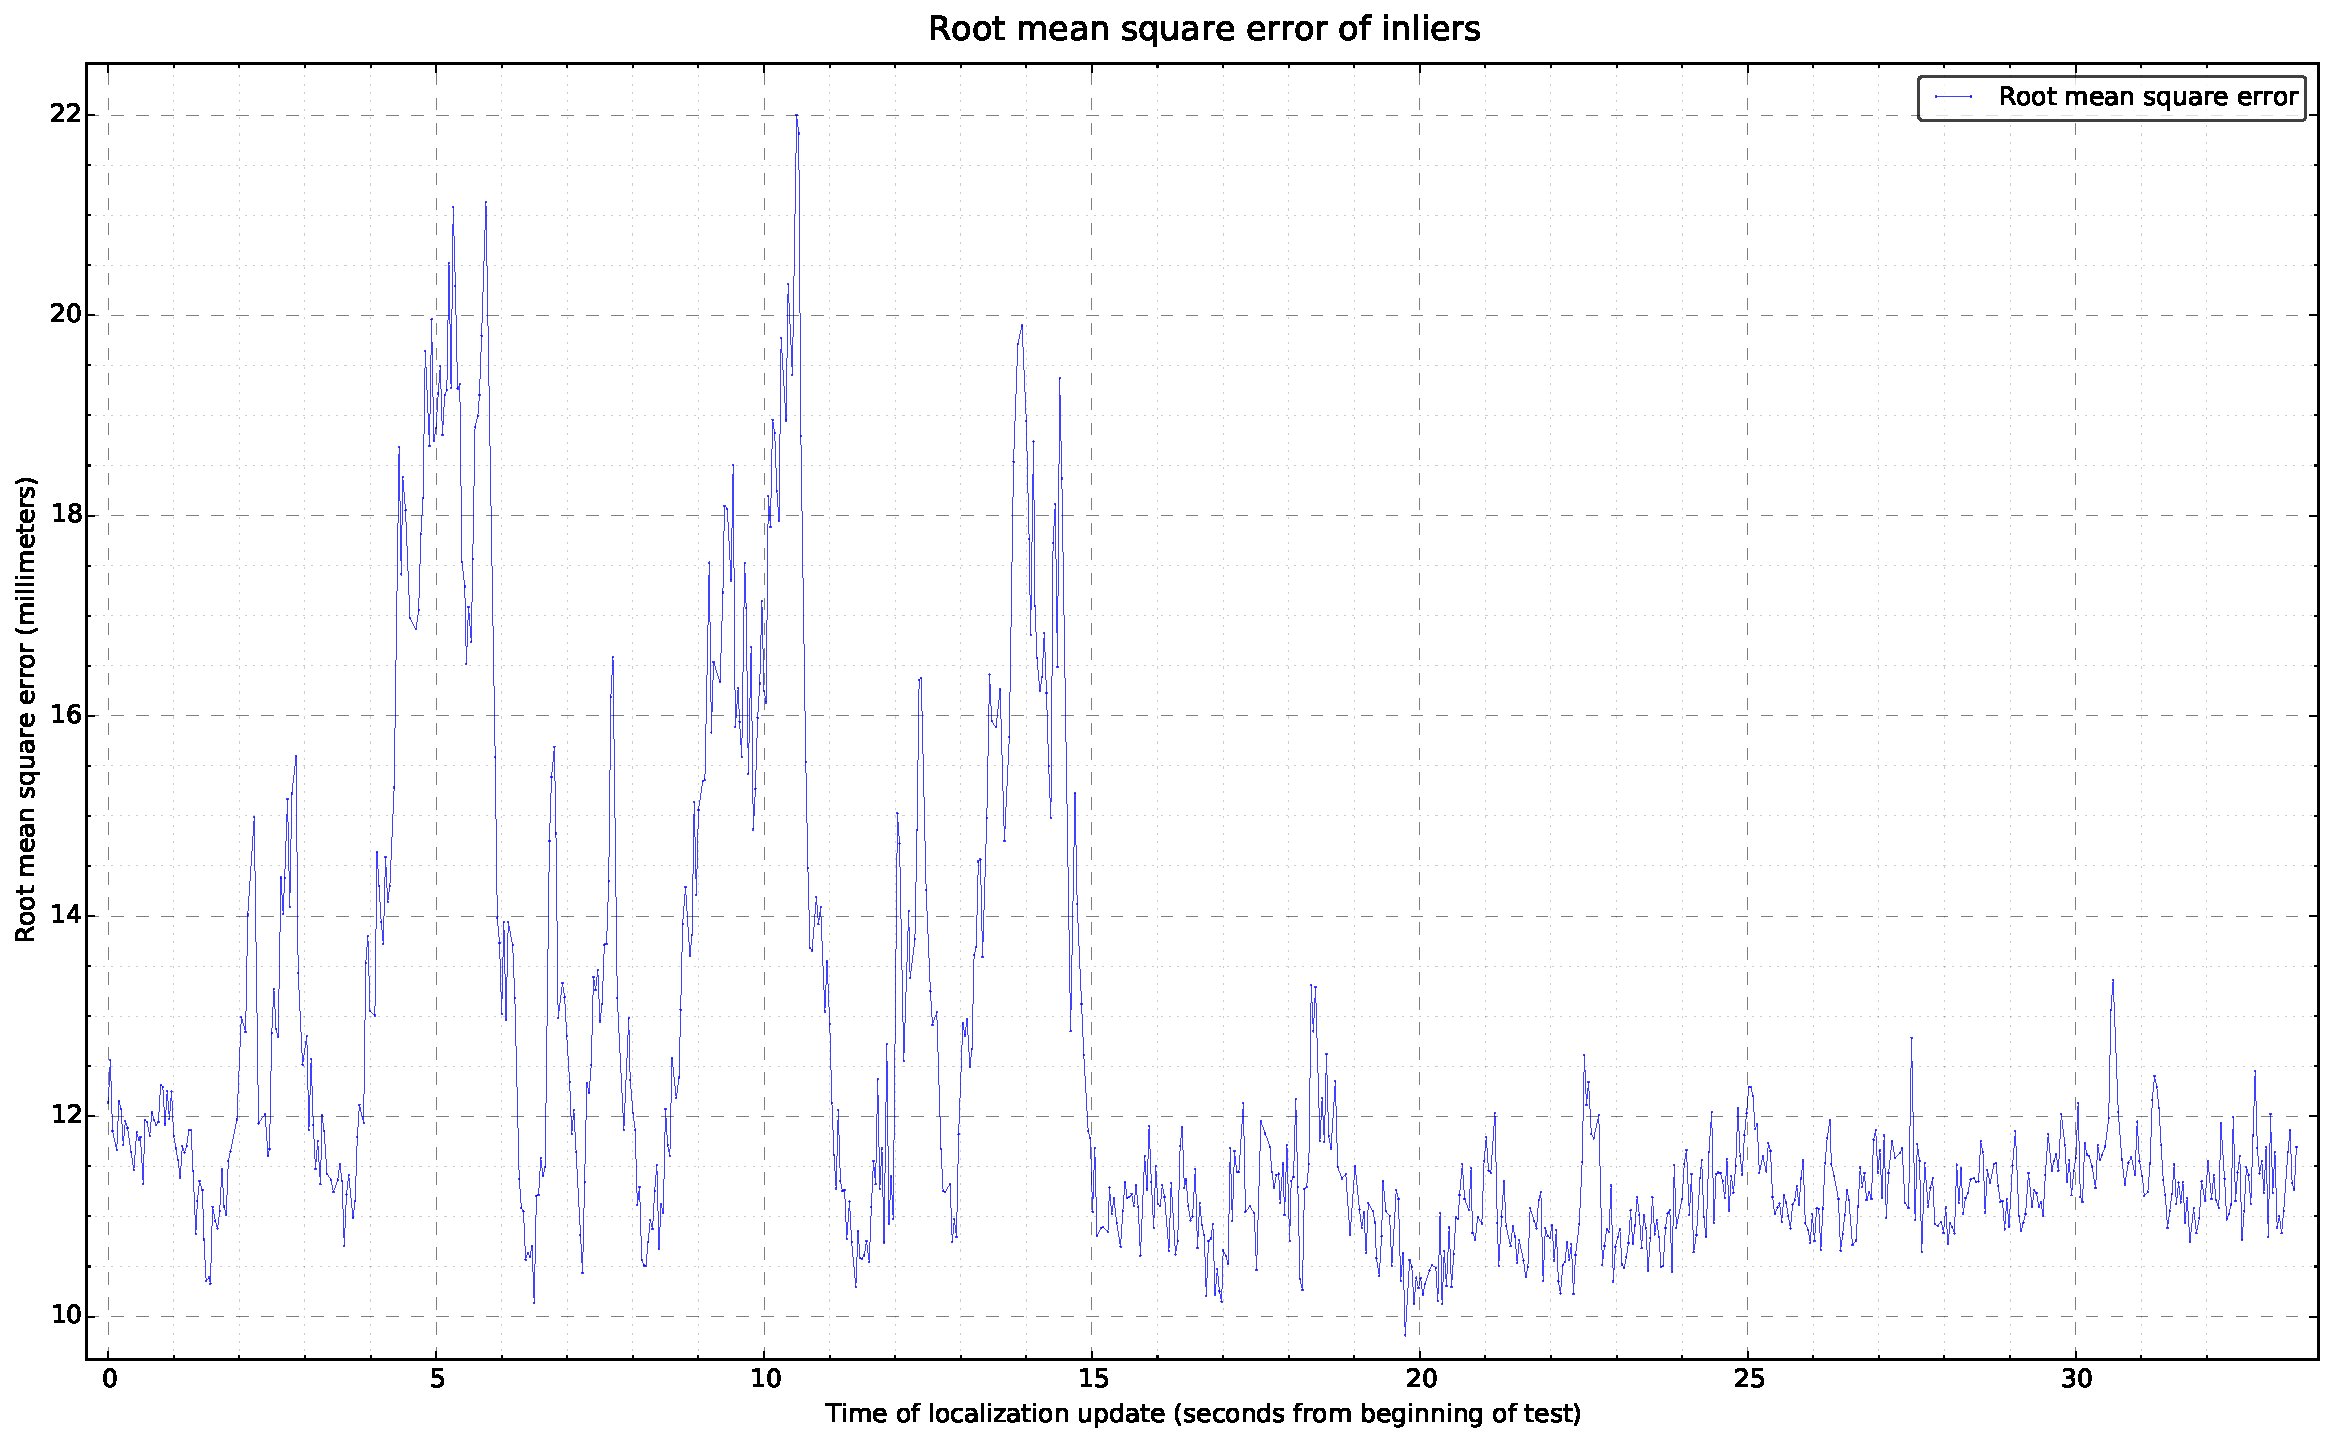
\includegraphics[width=0.69\textwidth]{appendices/tests-3dof/pioneer-robot/\currfilebase/graphs/root-mean-square-error-inliers}
	\caption{Root Mean Square Error of the inliers}
\end{figure}

\begin{figure}[H]
	\centering
	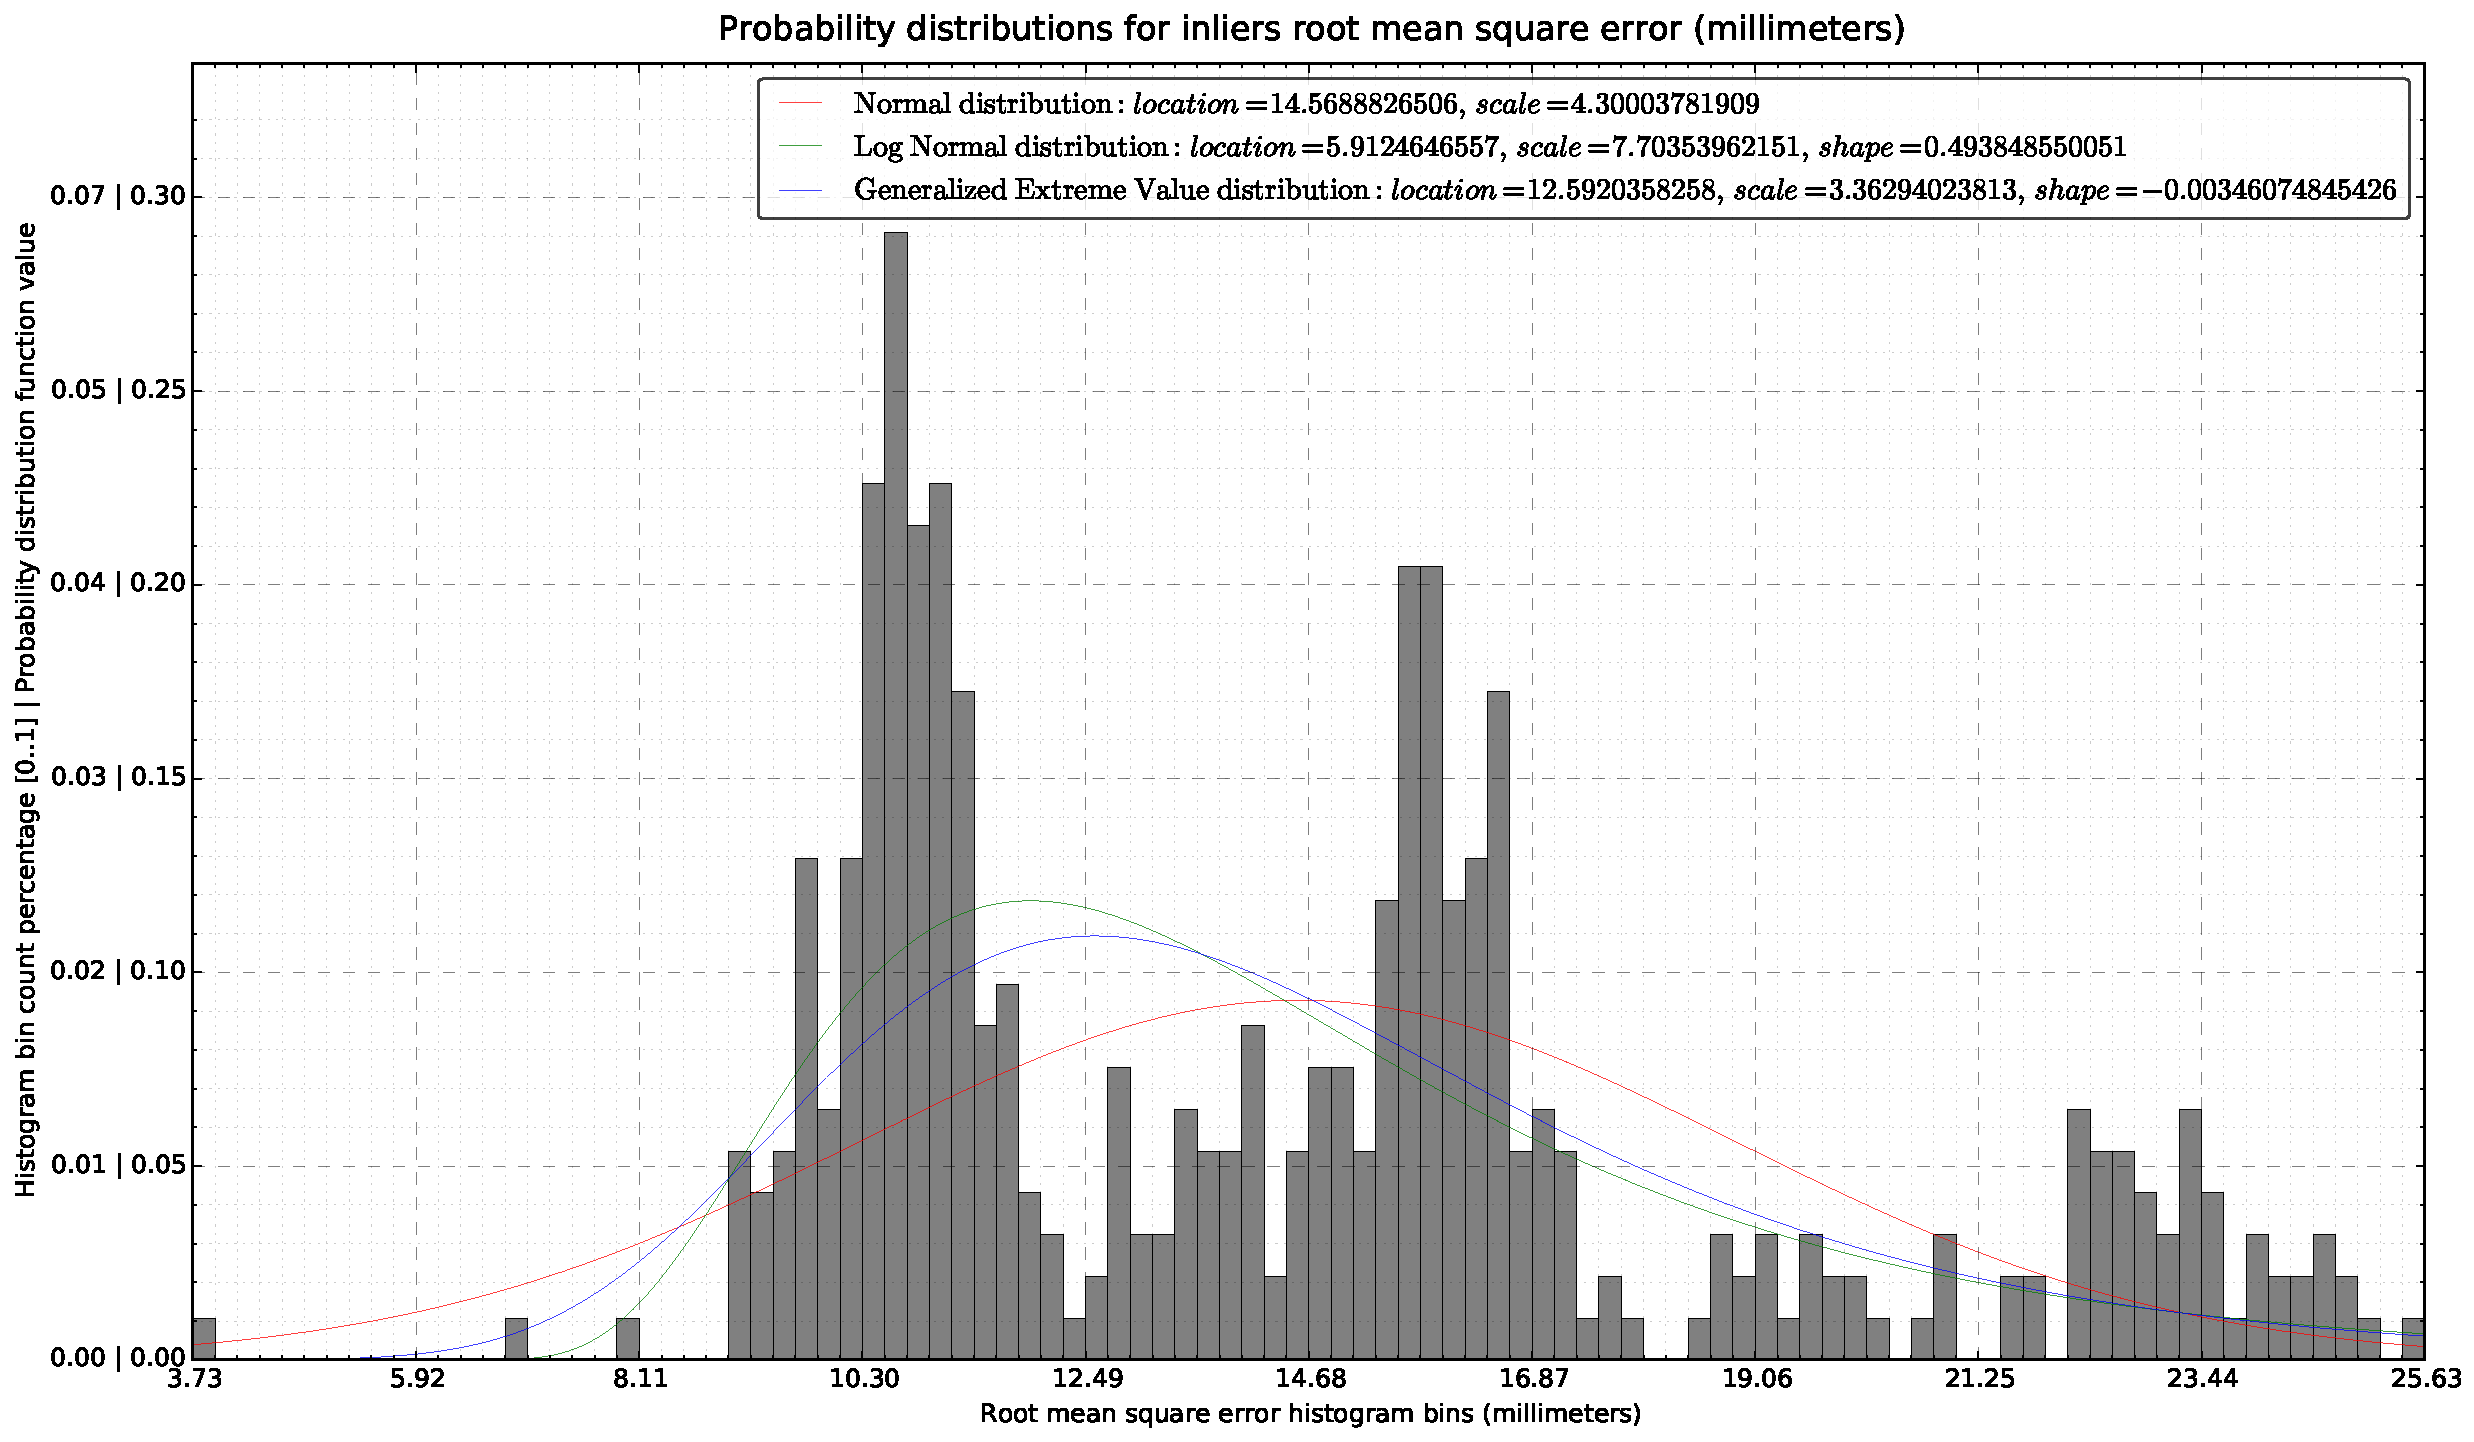
\includegraphics[width=0.69\textwidth]{appendices/tests-3dof/pioneer-robot/\currfilebase/graphs/root-mean-square-error-inliers-distributions}
	\caption{Probability distributions for the Root Mean Square Error of the inliers}
\end{figure}


%Computation times
\begin{figure}[H]
	\centering
	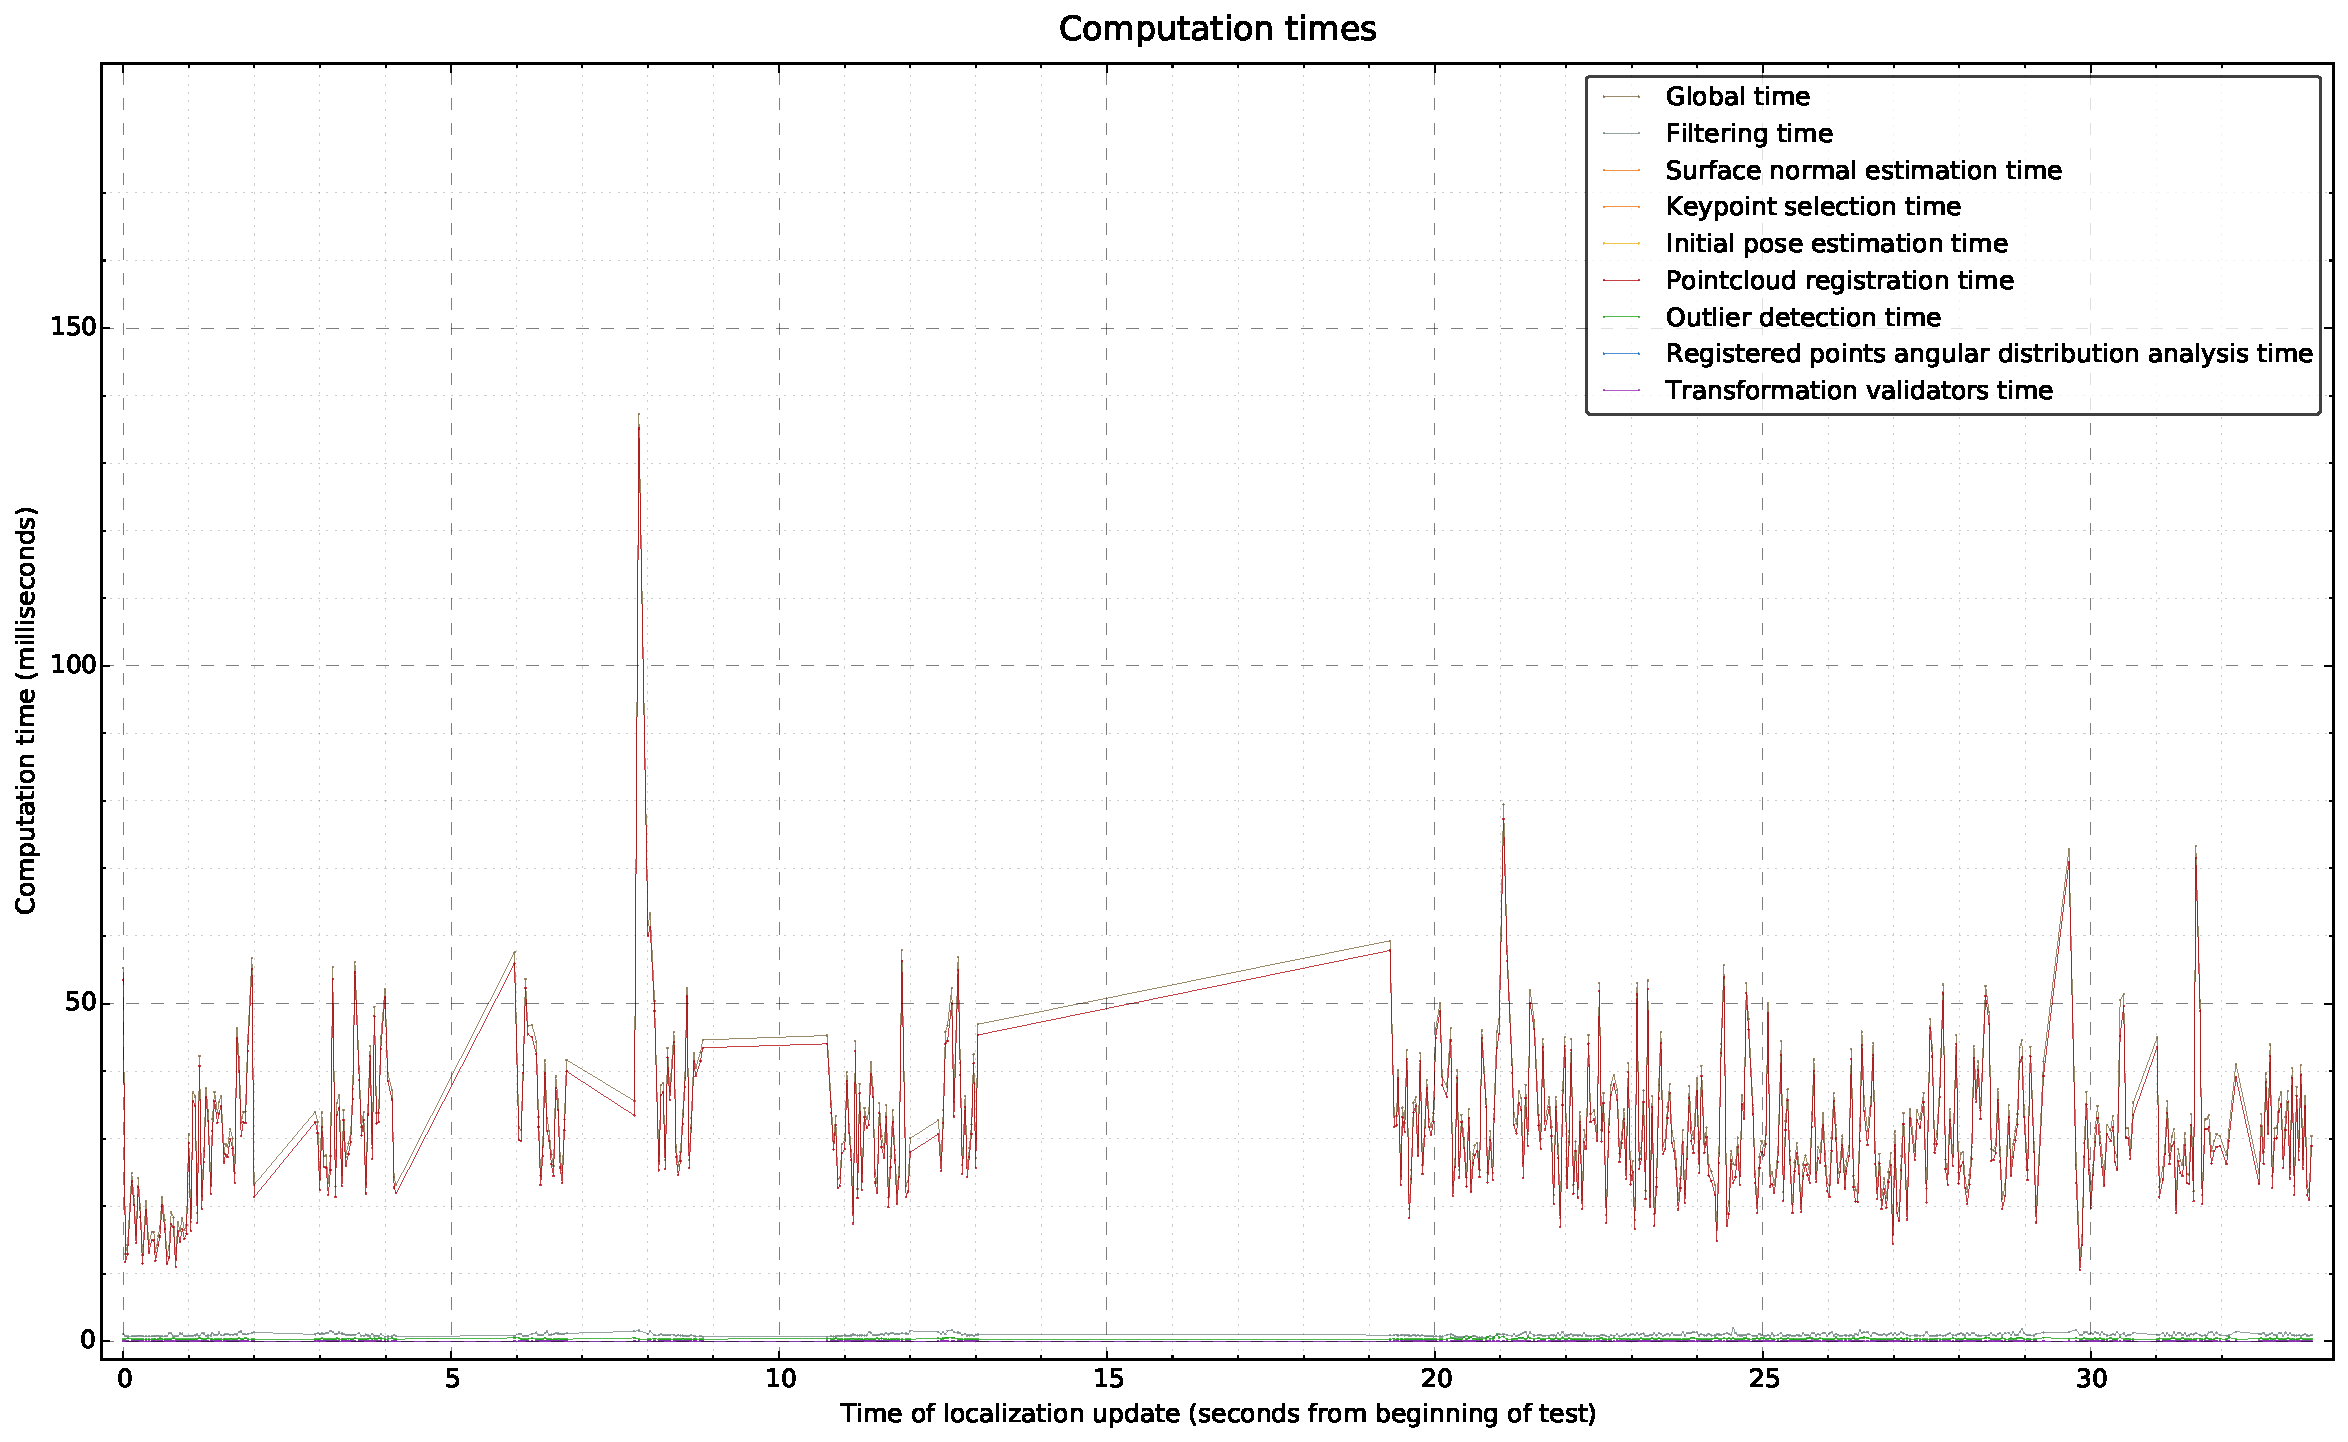
\includegraphics[width=0.69\textwidth]{appendices/tests-3dof/pioneer-robot/\currfilebase/graphs/computation-times-milliseconds}
	\caption{Localization system computation times}
\end{figure}

\begin{figure}[H]
	\centering
	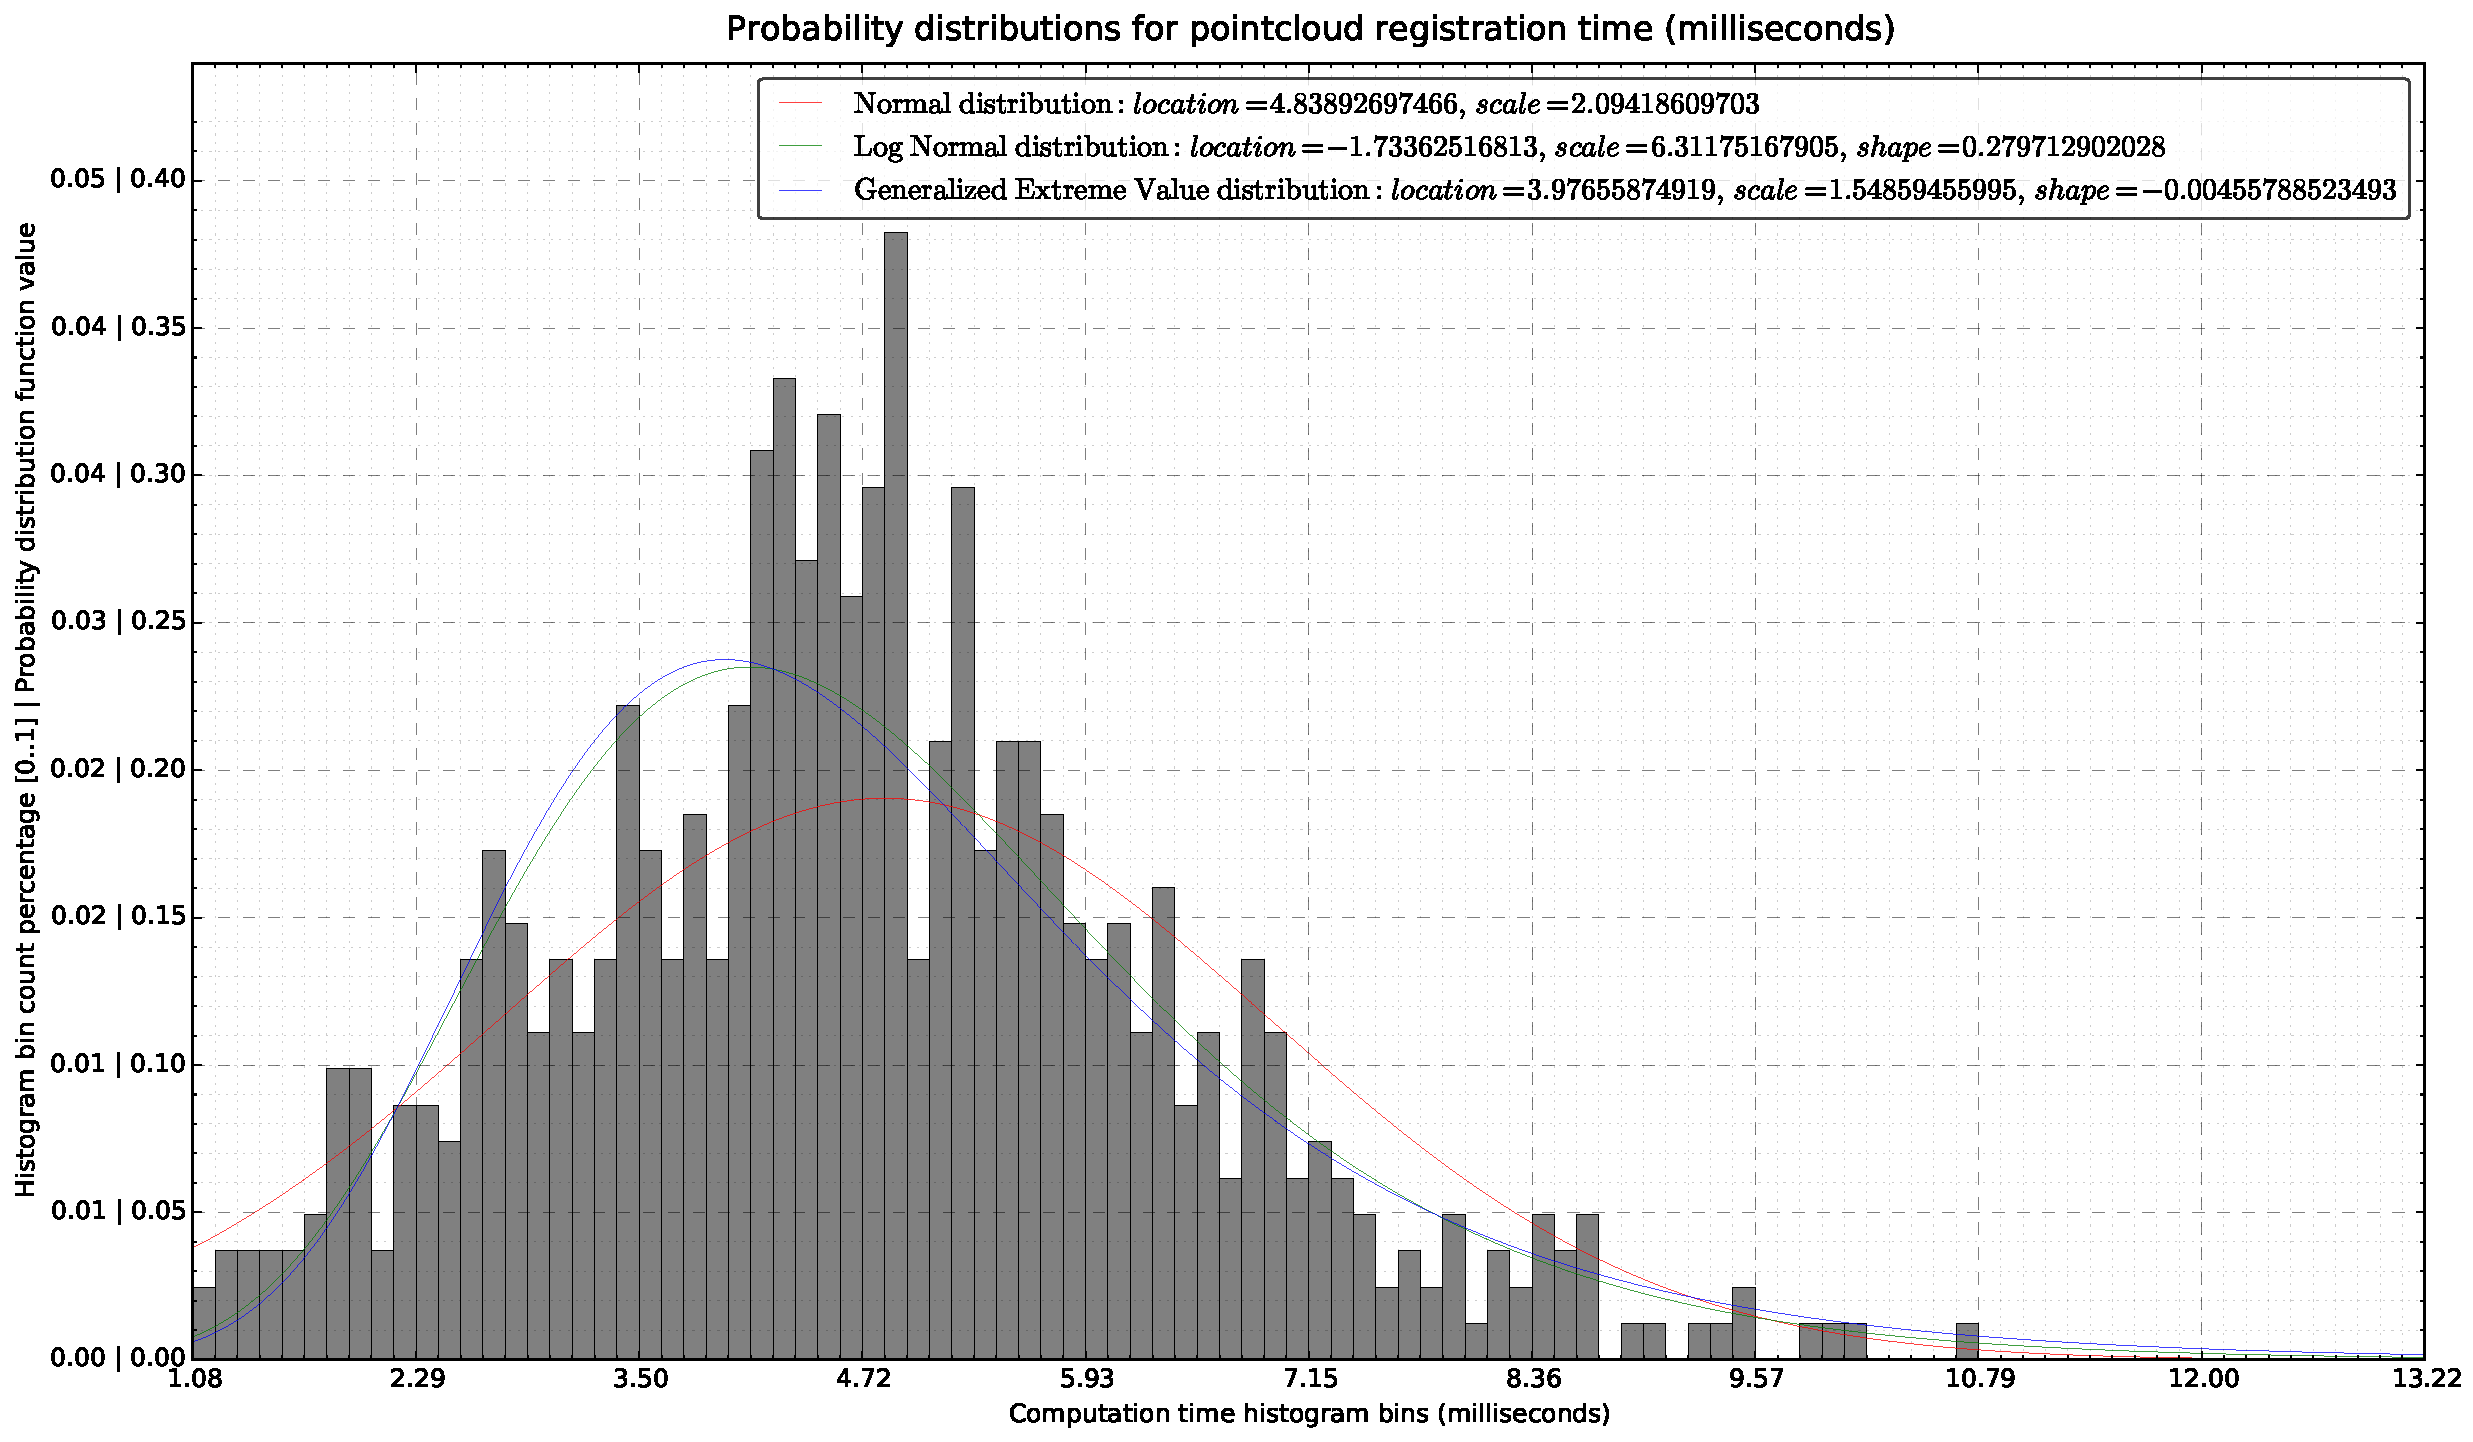
\includegraphics[width=0.69\textwidth]{appendices/tests-3dof/pioneer-robot/\currfilebase/graphs/computation-times-milliseconds-pointcloud-registration-time-distributions}
	\caption{Probability distributions for the point cloud registration time}
\end{figure}

\begin{figure}[H]
	\centering
	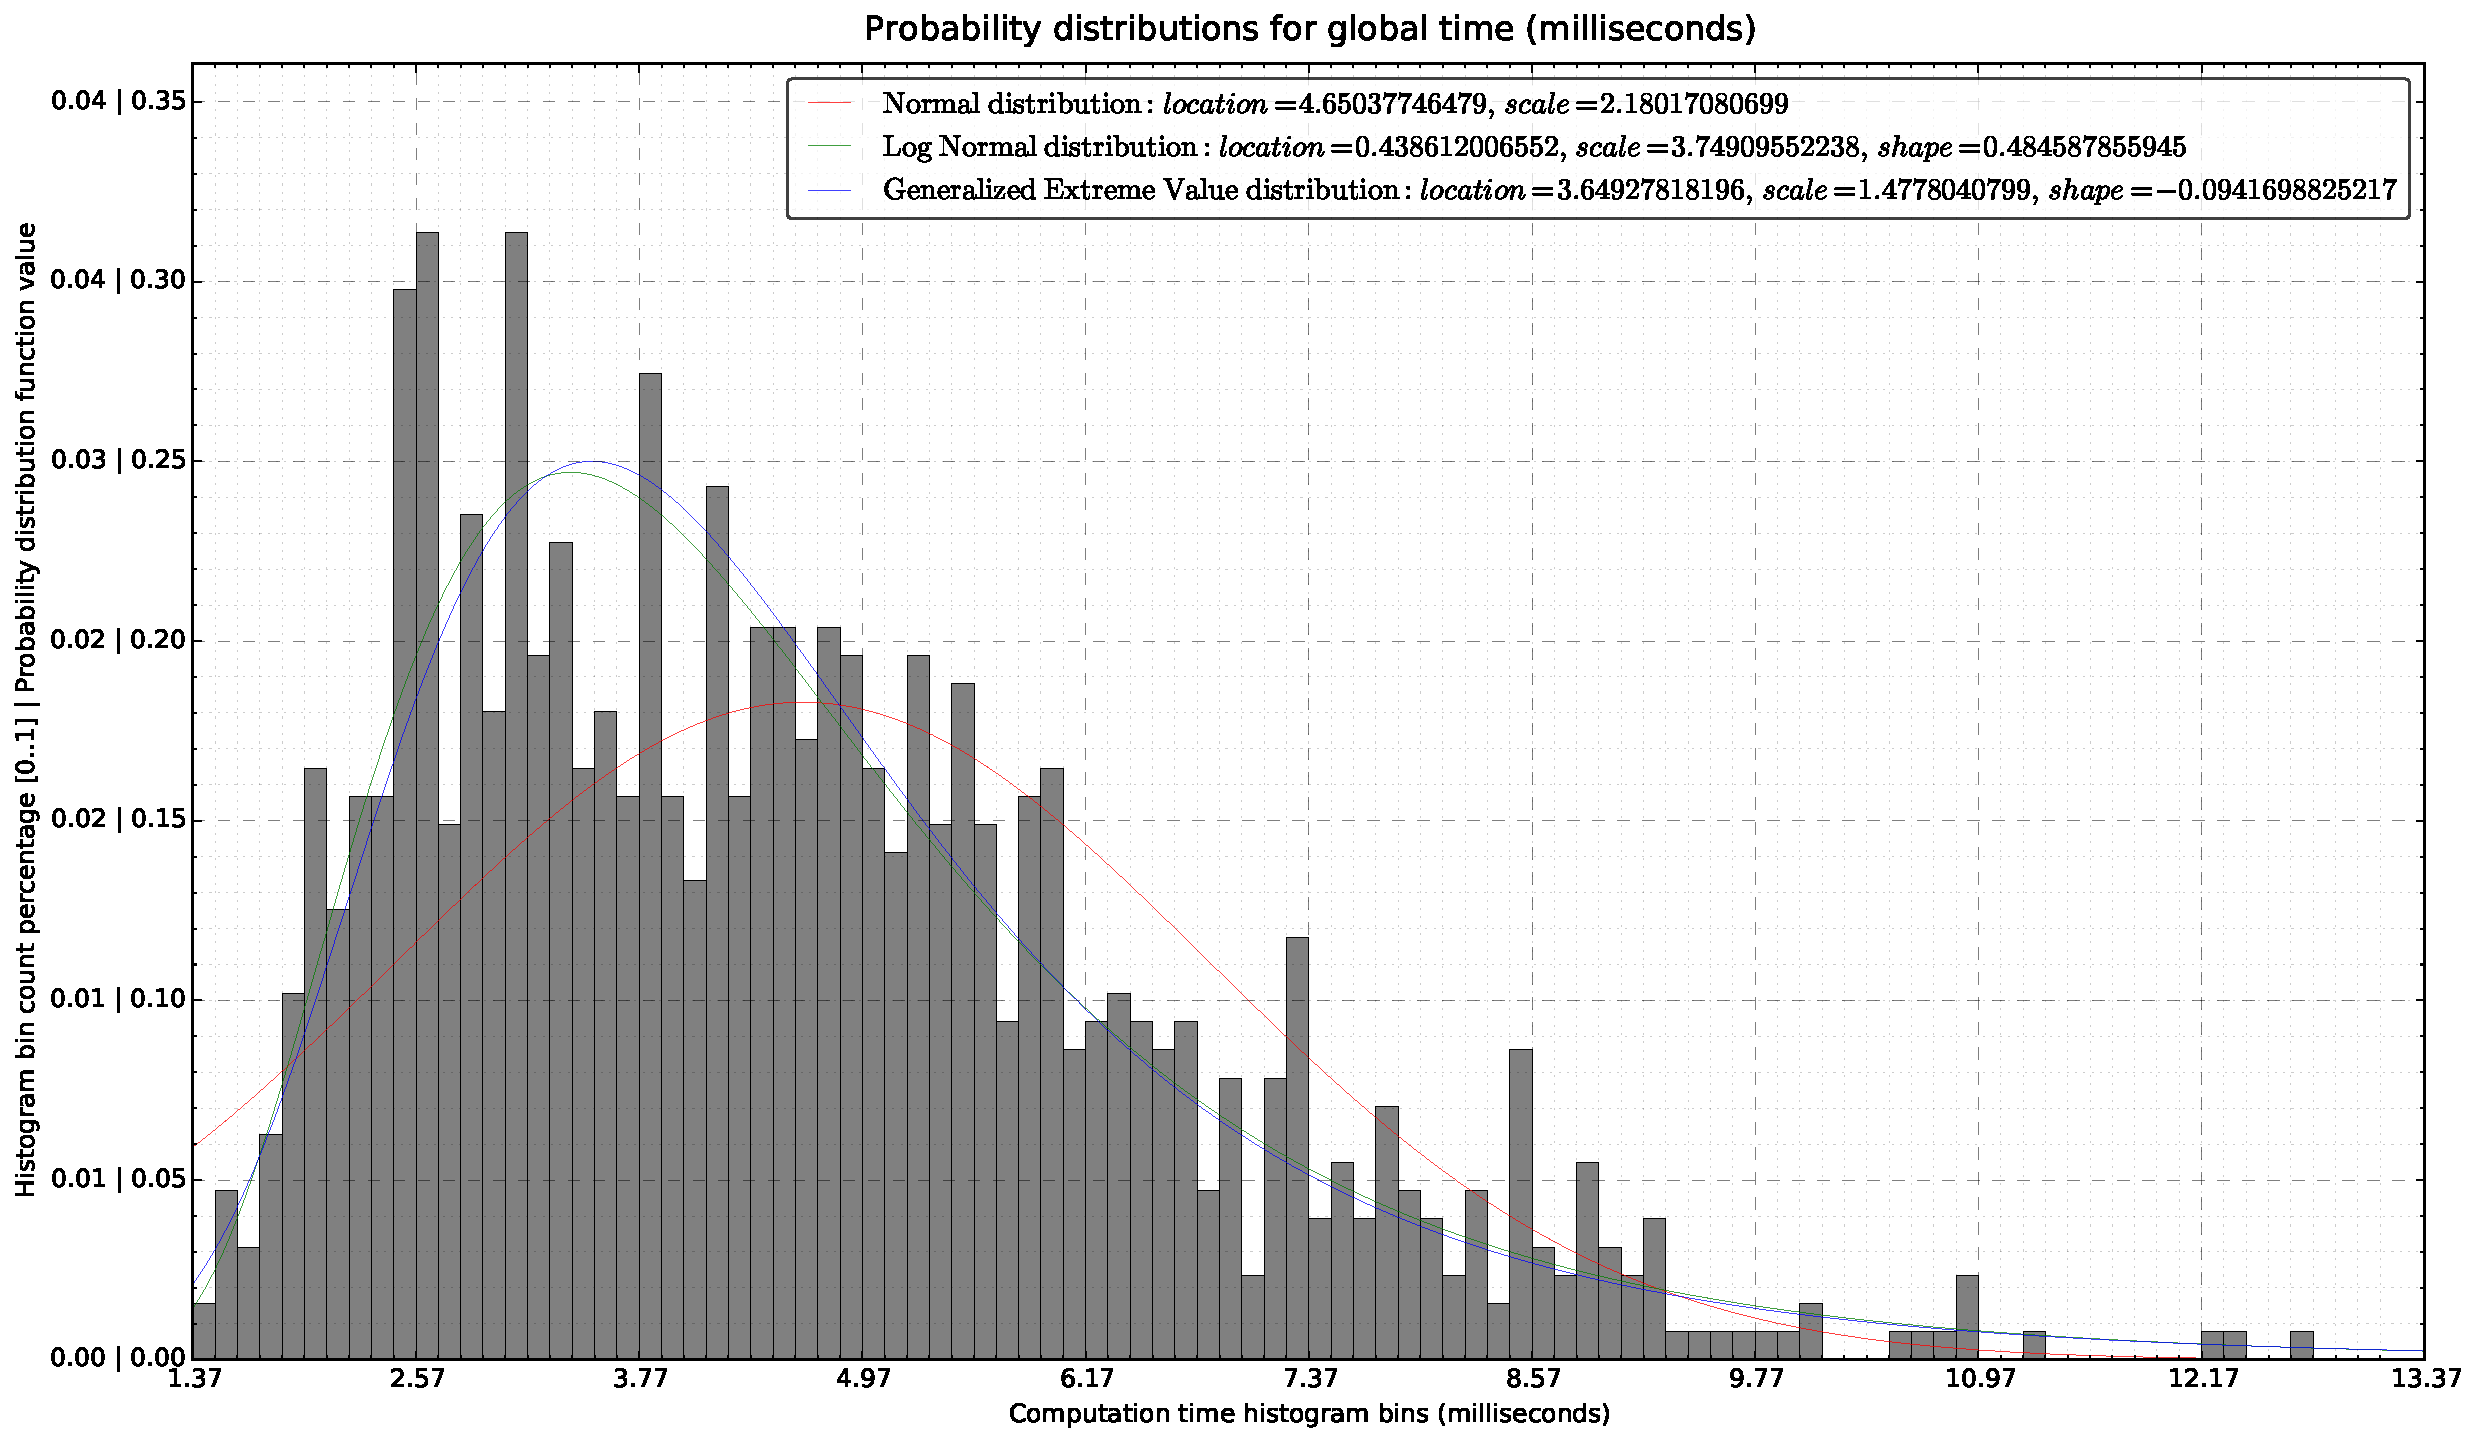
\includegraphics[width=0.69\textwidth]{appendices/tests-3dof/pioneer-robot/\currfilebase/graphs/computation-times-milliseconds-global-time-distributions}
	\caption{Probability distributions for the localization system global computation time}
\end{figure}
